\documentclass[letterpaper,11pt]{report}
\usepackage{epsfig,epstopdf}
\usepackage{float,captdef,multicol,amssymb,amsmath,amsfonts,fancybox}
\usepackage[activeacute,spanish]{babel}
%\usepackage[latin1]{inputenc}
\usepackage[colorlinks]{hyperref}

\usepackage{cancel}
\usepackage{marginnote}
\renewcommand*{\marginnotevadjust}{-0.1cm}
\renewcommand*{\marginfont}{\footnotesize}
%\renewcommand*{\marginfont}{\tiny}
\usepackage[right=4.5cm,left=2cm,top=2cm,bottom=2.0cm,headsep=0.7cm,footskip=1.0cm]{geometry}

%\usepackage[notref]{showkeys} % muestra los labels de las referencias.

\def\refname{Referencias}
\def\abstractname{Resumen}
\def\bibname{Referencias}
\def\chaptername{Cap{\'\i}tulo}
\def\appendixname{Ap'endice}
\def\contentsname{\'Indice}
\def\listfigurename{\'Indice de Figuras}
\def\listtablename{\'Indice de Tablas}
\def\indexname{\'Indice de Materias}
\def\figurename{Figura}
\def\tablename{Tabla}
\def\partname{Parte}
\def\enclname{Adjunto}
\def\ccname{Copia a}
\def\headtoname{A}
\def\headpagename{P\'agina}
\def\today{\number\day~de\space\ifcase\month\or
 enero\or febrero\or marzo\or abril\or mayo\or junio\or
 julio\or agosto\or septiembre\or octubre\or noviembre\or diciembre\fi
 \space de~\number\year}


%\topmargin -0.5cm  %regula margen superior (desde donde comienza a escribir)
%\headheight 10pt
%\headsep 0.6cm
%\textheight 22.5cm %regula el alto del texto



\begin{document}

\thispagestyle{empty}
\begin{center}

\

\vspace{6.5cm}

\rule{15cm}{0.1cm}

\vspace{1.5cm}

{\huge \textsc{\textbf{ELECTRODIN'AMICA I}}}

\vspace{1.5cm}

\rule{15cm}{0.1cm}

\vspace{1.5cm}

Versi'on del \today

\end{center}

\newpage
\thispagestyle{empty}
\ \\
\newpage
\setcounter{page}{1}
\pagenumbering{roman}

\pagestyle{plain}
\chapter*{Prefacio}
\addcontentsline{toc}{chapter}{Prefacio}
\bigskip
\bigskip
\bigskip
\bigskip
\bigskip
\bigskip


\emph{Este apunte ha sido escrito principalmente por \href{https://google.com/+GuillermoRubilar}{G. Rubilar} a partir de, e inspirado en, los cursos dictados por el Prof. Enrique Oelker en el Departamento de F'isica de la \href{www.udec.cl}{Universidad de Concepci\'on}, y ha contado con las contribuciones de F. Izaurieta, E. Rodriguez, J. Saez, C. Salas, O. Jim'enez, F. Torres, P. Mella, J. Oliva, P. Utreras, J. Villegas, P. Mu\~noz, M.A. Sol'is y A. Maldonado.}

\bigskip


\bigskip

Esta obra est'a publicada bajo una licencia Atribuci'on-No Comercial-Licenciar Igual 3.0 Chile de Creative Commons. Para ver una copia de esta licencia, visite
\url{http://creativecommons.org/licenses/by-nc-sa/3.0/cl/}.

\bigskip
\bigskip
\bigskip

\fbox{Otros apuntes en \url{https://sites.google.com/site/apuntesdecienciasfisicas}.}

\bigskip
\bigskip
\bigskip



\emph{\textquotedblleft ...As\'i, nosotros los mortales, somos
inmortales en lo que creamos en com\'un."}

\begin{flushright}
Albert Einstein.
\end{flushright}

\newpage

\tableofcontents
\pagenumbering{arabic}
\setcounter{page}{1}

\chapter{Electrost'atica}
\pagenumbering{arabic}
\setcounter{page}{1}

\section{Introducci'on y conceptos fundamentales}

Uno de los conceptos fundamentales para la descripci'on de los
fen'omenos electromagn'eticos es el de \textit{carga el'ectrica}.
La carga el'ectrica es una propiedad f'isica de los cuerpos,
atribuida a ellos precisamente para diferenciar (o, en general,
describir) su comportamiento en las interacciones
electromagn'eticas. La experiencia ha mostrado que es posible
describir las propiedades de la interacci'on
electromagn'etica (por ejemplo, atracci'on, repulsi'on, o ausencia de fuerza) si
se asume que la magnitud f'isica llamada carga el'ectrica puede
adoptar valores positivos, negativos (o nulos), y que es una
propiedad aditiva (es decir, que la carga el'ectrica total de un
sistema formado por otras cargas es la suma algebraica de las
cargas constituyentes).

En general, la interacci'on electromagn'etica entre cargas puede ser bastante complicada. Por ejemplo, la fuerza que una carga ejerce sobre otra depende en general no s'olo de la distancia entre ellas, sino tambi'en de sus velocidades y aceleraciones relativas, y presenta adem'as efectos ``de retardo'' (esto quiere decir que la fuerza que una carga experimenta debido a la otra no depende de la posici'on, velocidad y aceleraci'on de la otra en el mismo instante, sino que en tiempos anteriores). Por esto, comenzaremos estudiando el caso m'as simple en que el sistema de cargas consideradas es \textit{estacionario}. En esta situaci'on los efectos de retardo y la dependencia con las velocidades y aceleraciones desaparecen, de modo que \textbf{las fuerzas electrost'aticas dependen s'olo de las distancias entre las cargas}.


\subsection{Ley de Coulomb}

En 1785 Coulomb\footnote{Charles Augustin de Coulomb: f'isico e ingeniero franc'es (1736-1806). Ver \url{http://es.wikipedia.org/wiki/Charles-Augustin_de_Coulomb}.} \textit{establece experimentalmente} que la fuerza entre dos cargas muy peque\~nas comparadas con la distancia que las separa (``puntuales'') es \textit{aproximadamente}  proporcional a la magnitud de las cargas, inversamente proporcional al cuadrado de la distancia entre ellas y en la direcci'on que las
une. Finalmente el sentido de la fuerza es tal que dos cargas de igual signo se repelen y dos de signos opuestos se atraen. Este resultado experimental, y por consiguiente necesariamente aproximado, es la base de la teor'ia de la interacci'on electrost'atica. Esta teor'ia \textit{asume} entonces que la fuerza entre cargas ``puntuales'' es \textit{exactamente} inversamente proporcional al cuadrado de la distancia que las separa y en la direcci'on de la l'inea que los une, de modo que
\begin{center}
\begin{figure}[H]
\centerline{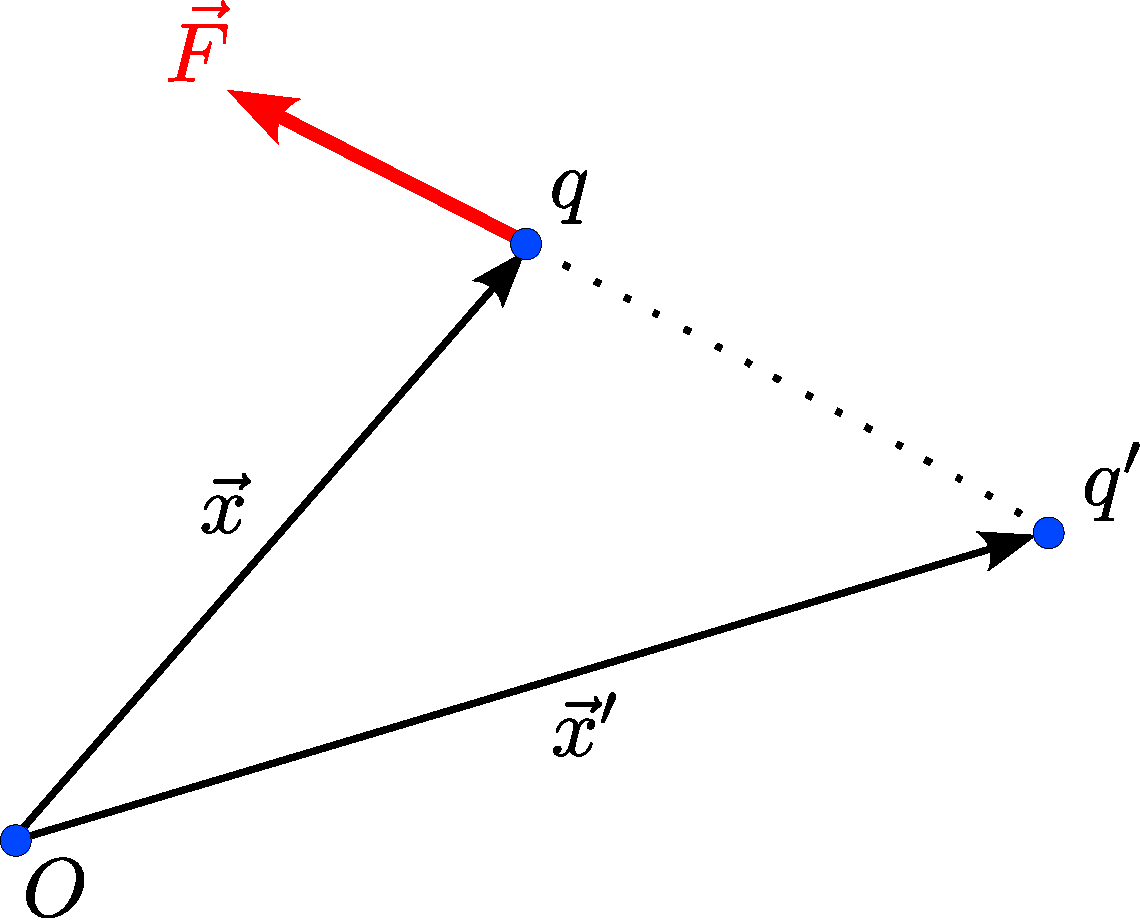
\psfig{file=fig/fig-Coulomb.pdf,height=4cm,angle=0}}
\caption{Fuerza electrost'atica entre dos cargas puntuales.}
\label{fig:Coulomb}
\end{figure}
\end{center}
\begin{equation}
F_i\propto \underbrace{\frac{qq'}{\left\vert \vec x-\vec
x'\right\vert^2}}_\text{magnitud}\cdot
\underbrace{\frac{x_i-x_i'}{\left\vert \vec x-\vec x'\right\vert }}_\text{vector unitario}.
\end{equation}
Podemos por tanto escribir
\begin{equation}
F_i=k\frac{qq'}{\left\vert \vec x-\vec x'\right\vert^2}
\cdot\frac{x_i-x_i'}{\left\vert \vec x-\vec x'\right\vert }.
\end{equation}
El valor de la constante $k$ depende del sistema de unidades usado para medir
magnitud de las cargas el'ectricas. Nosotros utilizaremos el sistema internacional SI (MKSA) donde la constante $k$ es denotada como\footnote{En el \textit{sistema gaussiano de unidades} (cgs) se
define $k:=1$ de modo que la unidad de carga no es independiente:
$[q]\stackrel{\text{cgs}}{=}cm^{3/2}g^{1/2}s^{-1}$. Esta unidad es llamada una
\textit{unidad electrost'atica} (esu) o un \textit{statCoulomb}.}%
\begin{equation}
k:=\frac{1}{4\pi\varepsilon_0},
\end{equation}
y donde $\varepsilon_0$ se conoce como la \textit{permitividad del vac\'{\i}o}, y
entonces
\begin{equation}\marginnote{Ley de Coulomb}
\boxed{F_i=\frac{qq'}{4\pi\varepsilon_0}\frac{\left(  x_i-x_i^{\prime
}\right)  }{\left\vert \vec x-\vec x'\right\vert ^3}.}\label{leycoulomb}%
\end{equation}
En el sistema SI, la constante
$k$ tiene el valor
\begin{equation}
k=c^2\times 10^{-7}\ Nm^2C^{-2},
\end{equation}
en que $c$ es la \textit{velocidad de la luz en el vac\'{\i}o}. Su valor es
$c=2.99792458\times 10^{8}\,ms^{-1}$. Con esto $k\approx 9.0\times
10^{9}\,Nm^2C^{-2}$, $\varepsilon _0\approx 8.854\times 10^{-12}
\,C^2N^{-1}m^{-2}$.

La expresi'on \eqref{leycoulomb} es conocida como \textit{ley de Coulomb}.
Adicionalmente, se \textit{asume} que la fuerza que ejerce un conjunto de $N$
cargas puntuales $q^{(\alpha)}$, $\alpha=1,\cdots N$, en posiciones $x^{(\alpha)}_i$ sobre una carga $q$ con posici'on $x_i$ es
\begin{equation}
F_i   =\sum_{\alpha=1}^{N}\frac{qq^{(\alpha)}}{4\pi\varepsilon_0}\frac{\left(
x_i-x^{(\alpha)}_i\right)  }{\left\vert  \vec x-\vec x^{(\alpha)}\right\vert^3}
=\frac{q}{4\pi\varepsilon_0}\sum_{\alpha=1}^{N}q^{(\alpha)}\frac{\left(
x_i-x^{(\alpha)}_i\right) }{\left\vert  \vec x-\vec
x^{(\alpha)}\right\vert^3}.\label{leycoulomb-discre}
\end{equation}
La suposici'on que esta fuerza sea la suma (vectorial) de las fuerzas individuales que
actuar'ia sobre la carga $q$ debido a cada una de las cargas $q^{(\alpha)}$ es
llamado \textit{principio de superposici'on}. Note que, como su nombre lo indica, este es un \textit{principio} en el que se basa la teor'ia electromagn'etica, ya que no es \textit{necesario a priori} que la interacci'on electrost'atica respete esta propiedad. En otras palabras, podr'ia ocurrir (o haber ocurrido) que la fuerza que dos cargas ejercen sobre una tercera no fuese \textit{exactamente} la suma vectorial de las fuerzas que cada una de ellas ejerce individualmente. Por ejemplo, hoy sabemos que esto 'ultimo es lo que efectivamente ocurre con la interacci'on gravitacional (!`\textit{no} satisface el principio de superposici'on!). En la teor'ia electromagn'etica se asume que la superposici'on es satisfecha en forma exacta. Como veremos, una consecuencia de este principio es que las ecuaciones que relacionan los campos el'ectricos (y sus respectivas fuerzas) con las distribuciones de carga que las producen est'an descritas por \textit{ecuaciones} (diferenciales y/o integrales) \textit{lineales}.


Para una \textit{distribuci'on continua de cargas} podemos considerar un elemento de
volumen $dV'$ conteniendo una carga $dq'=\rho(x')dV'$, donde $\rho(x')$ es
la densidad (volum'etrica) de carga (carga por unidad de volumen). Usando el
principio de superposici'on podemos escribir la fuerza total que esta
distribuci'on ejerce sobre una carga (puntual) de prueba $q$ como
\begin{align}
F_i  &= \int_V dF_i \\
& =\int_V\frac{q}{4\pi\varepsilon_0}\frac{\left(  x_i-x_i^{\prime
}\right)  }{\left\vert \vec x-\vec x'\right\vert ^3}dq^{\prime},
\end{align}
es decir,
\begin{equation}\marginnote{Fza. sobre carga puntual}
F_i  =\frac{q}{4\pi\varepsilon_0}\int_V\rho(x')\frac{\left(x_i-x_i'\right)
}{\left\vert \vec x-\vec x'\right\vert
^3}dV' .\label{leycoulomb-conti}
\end{equation}
An'alogamente, podemos describir cargas distribuidas en (regiones que puedan
aproximarse por) una superficie y/o curva usando la \textit{densidad superficial de
carga} $\sigma(x')$ (carga por unidad de 'area) y/o la \textit{densidad lineal de carga} $\lambda(x')$ (carga por unidad de longitud), de modo que $dq'=\sigma(x')dS$
y $dq'=\lambda(x')d\ell$, respectivamente.

\subsection{Campo el'ectrico}
El campo el'ectrico $E_i(\vec{x})$ en un punto $x_i$ es definido operacionalmente como la fuerza por unidad de carga \textit{sobre una carga muy peque\~na en tama\~no y magnitud} (``carga de prueba puntual'') $q$ situada en la posici'on $x_i$, es decir,
\begin{equation}
E_i(\vec x):=\lim_{q\rightarrow0}\frac{F_i}{q}.
\end{equation}
Note que el proceso l'imite ${q\rightarrow0}$ es necesario puesto que el uso de una carga $q$ de forma y magnitud arbitraria en general (mediante la fuerza de Coulomb) \textit{modificar'a la distribuci'on de cargas original}. Si la carga $q$ es cada vez m'as peque\~na en extensi'on y magnitud, entonces 'esta modificar'a cada vez menos la distribuci'on de carga original. En el l'imite ${q\rightarrow0}$, que ciertamente es una abstracci'on ya que en la pr'actica no existen cargas puntuales, ni tampoco cargas de magnitud arbitrariamente peque\~na, el cuociente $F_i/q$ ser'a independiente de la carga de prueba usada, y describir'a por lo tanto una cantidad dependiente s'olo de la distribuci'on de cargas considerada. Esto permite entonces considerar al campo el'ectrico como el campo \textit{generado por la distribuci'on de cargas}.

Con estas consideraciones, tenemos entonces que el campo el'ectrico generado por un conjunto de cargas puntuales $q^{(\alpha)}$ es dado por
\begin{equation}\marginnote{C. el'ectrico, cargas puntuales}
E_i(\vec x)=\frac{1}{4\pi\varepsilon_0}\sum_{\alpha=1
}^{N}q^{(\alpha)}\frac{\left(  x_i-x^{(\alpha)}_i\right)  }{\left\vert
\vec x-\vec x^{(\alpha)}\right\vert ^3}.\label{campelectr}
\end{equation}
Similarmente, para una distribuci'on volum'etrica de cargas:
\begin{equation}\marginnote{C. el'ectrico, distribuci'on}
\boxed{E_i(\vec x)=\frac{1}{4\pi\varepsilon_0}\int_V\rho(x')\frac{\left(
x_i-x_i'\right)  }{\left\vert \vec x-\vec x'\right\vert
^3}dV'.} \label{cerho}
\end{equation}
En general, preferiremos la descripci'on de la distribuci'on de cargas en t'erminos de la densidad volum'etrica $\rho(\vec{x})$, ya que a partir de ella podemos recobrar r'apidamente los otros casos de inter'es. Por ejemplo, podemos recobrar el resultado para el conjunto de cargas puntuales \eqref{campelectr} a partir de 
\eqref{cerho} si consideramos
\begin{equation}
\rho(\vec x)=\sum_{\alpha=1}^{N}q^{(\alpha)}\delta^{(3)}\left(\vec x-\vec
x^{(\alpha)}\right).
\label{conti-discre}
\end{equation}

\subsection{L'ineas de campo el'ectrico}
En electrodin'amica es 'util introducir el concepto de \textit{l'ineas de campo}. En el caso electrost'atico, asociado a cada configuraci'on de campo el'ectrico, descrito por el campo $E_i(\vec{x})$, es posible definir l'ineas de campo el'ectrico. Cada una de estas curvas, puede modelarse usando una parametrizaci'on de la forma $x_i=x_i(\lambda)$, donde $\lambda$ es un par'ametro real. Las l'ineas de campo son definidas como aquellas tales que sus vectores tangentes en cada punto son paralelos al vector campo el'ectrico. Esto es equivalente a la condici'on,
\begin{equation}\marginnote{L'ineas de campo}
\frac{dx_i}{d\lambda}(\lambda)=E_i(\vec{x}(\lambda)). \label{dlc}
\end{equation}
Note que, en general, es posible considerar un factor adicional al lado derecho de esta expresi'on (por ejemplo, $\alpha(\lambda)E_i(\vec{x}(\lambda))$ en lugar de $E_i(\vec{x}(\lambda))$), sin embargo la funci'on $\alpha(\lambda)$ puede siempre ser ``normalizada'' al valor $1$ redefiniendo convenientemente el par'ametro para describir la curva.

M'as expl'icitamente, la condici'on (\ref{dlc}) adopta, en coordenadas cartesianas y en tres dimensiones, la forma 
\begin{align}
\frac{dx}{d\lambda}(\lambda) &= {E_x}(x(\lambda),y(\lambda),z(\lambda)), \\
\frac{dy}{d\lambda}(\lambda) &= {E_y}(x(\lambda),y(\lambda),z(\lambda)),\\
\frac{dz}{d\lambda}(\lambda) &= \vec{E_z}(x(\lambda),y(\lambda),z(\lambda)),
\end{align}
de modo que define, dadas las componentes del campo $E_x(x,y,z)$, $E_y(x,y,z)$ y $E_y(x,y,z)$, un sistema de 3 ecuaciones diferenciales ordinarias acopladas, de primer orden, para las inc'ognitas $x(\lambda),y(\lambda)$ y $z(\lambda)$.

Una l'inea de campo particular queda determinada por la soluci'on del sistema de ecuaciones que satisface una determinada condici'on inicial, por ejemplo $\vec{x}(0)=\vec{x}_0$, donde $\vec{x}_0$ es un punto dado del espacio. La correspondiente soluci'on $\vec{x}(\lambda;\vec{x}_0)$ describir'a la l'inea de campo que pasa por el punto $\vec{x}_0$. Para algunos ejemplos, ver la figura\footnote{Figuras generadas usando VectorFieldPlot \cite{VFP}.} \ref{fig-E}.

\begin{center}
\begin{figure}[H]
\centerline{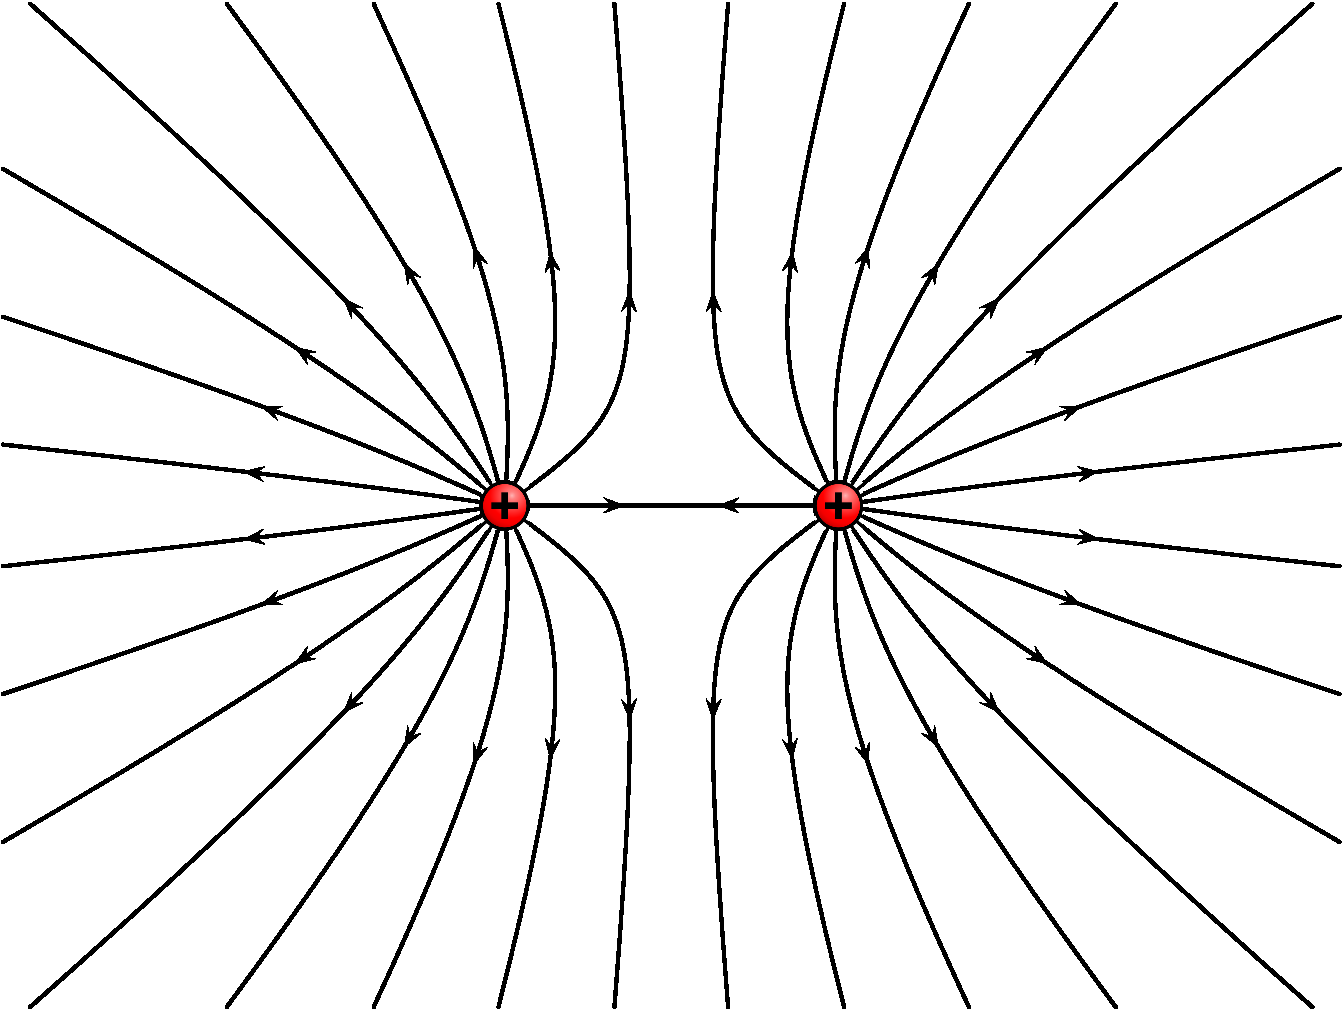
\psfig{file=fig/fig-E-01.pdf,height=4cm,angle=0}\hfill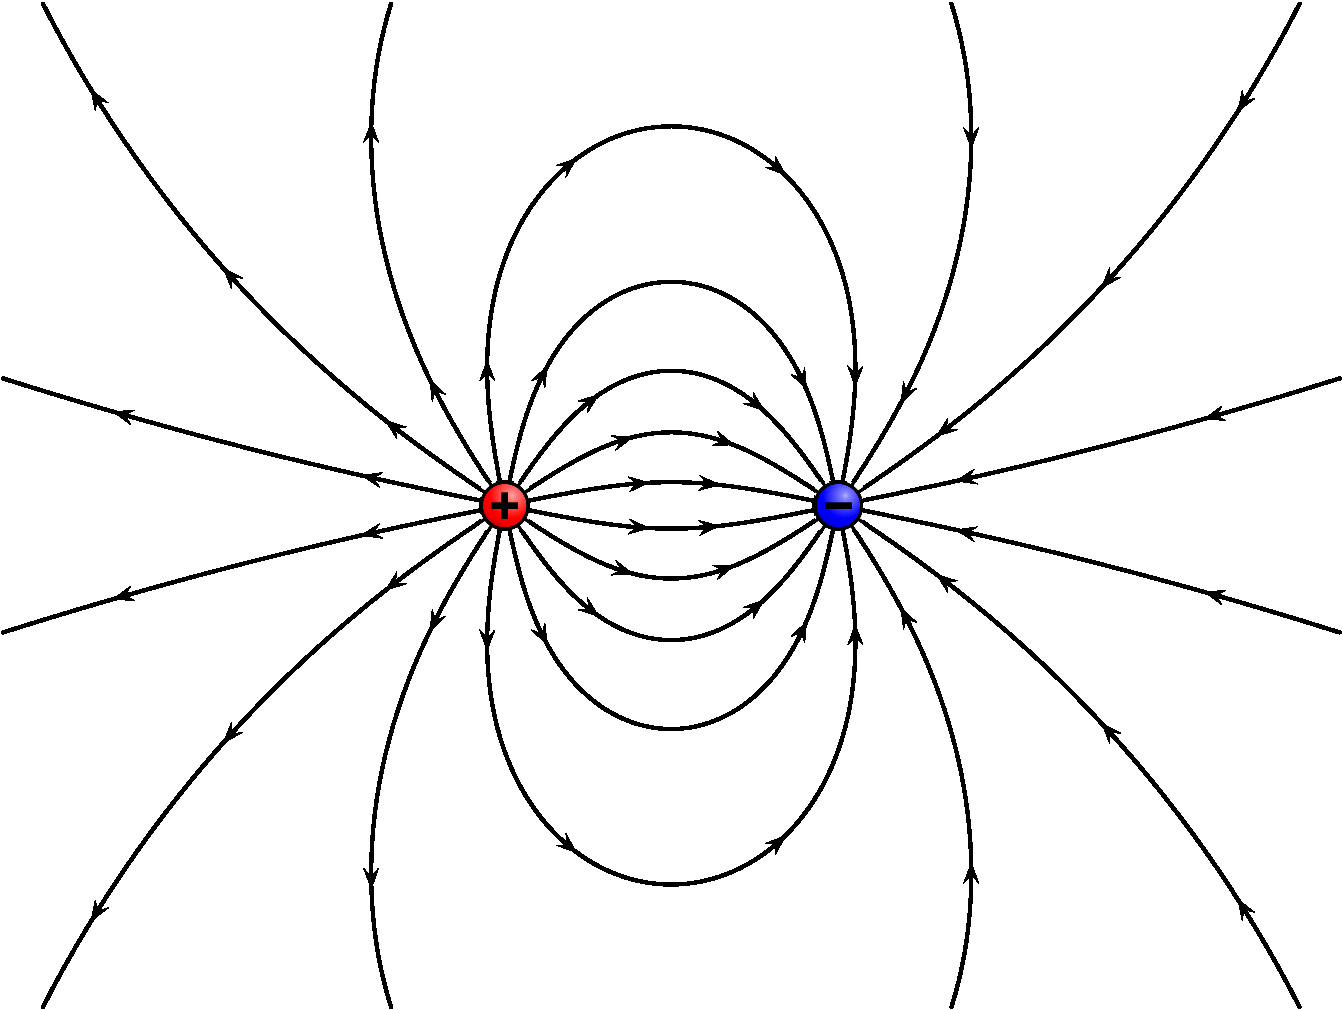
\psfig{file=fig/fig-E-02.pdf,height=4cm,angle=0}\hfill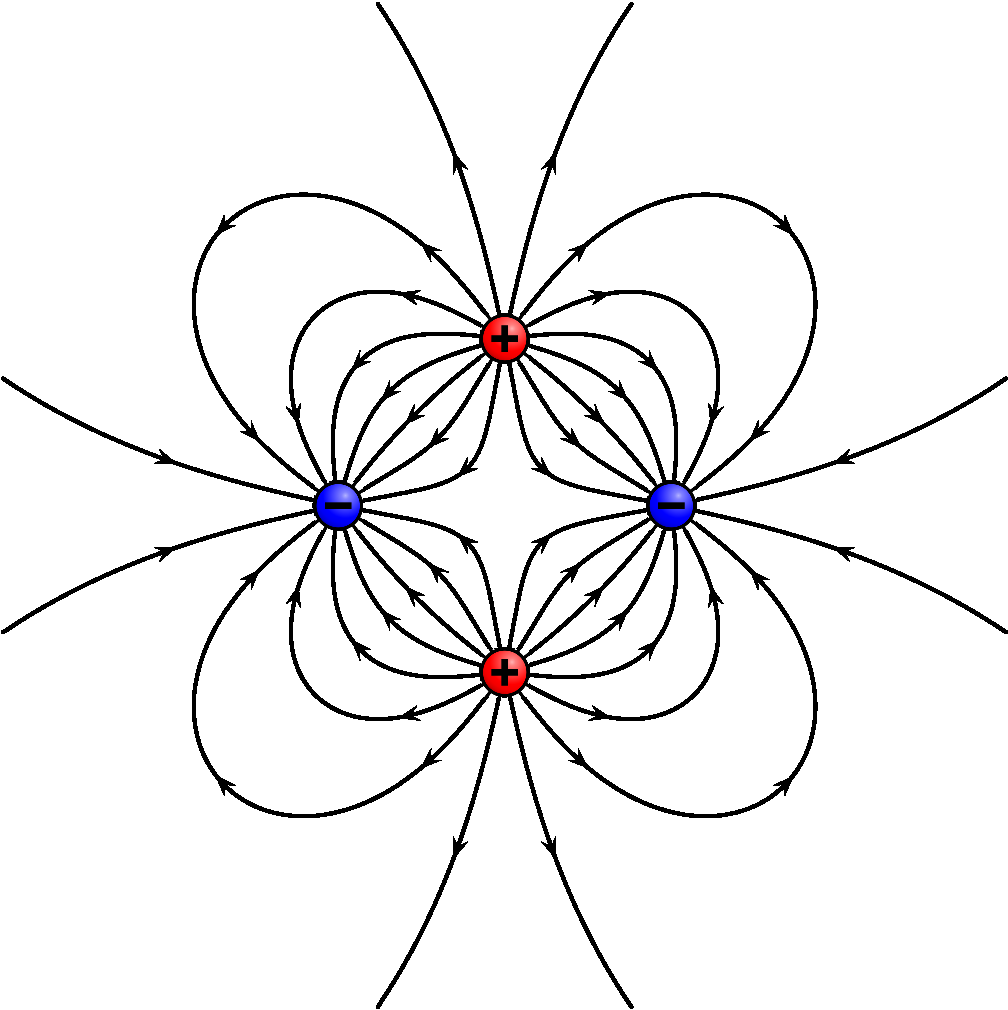
\psfig{file=fig/fig-E-03.pdf,height=4cm,angle=0}}
\caption{Ejemplos simples de l'ineas de campo el'ectrico.}
\label{fig-E}
\end{figure}
\end{center}
\subsection{Potencial el'ectrico}
Usando el hecho que
\begin{equation}
\frac{x_i-x_i'}{\left\vert \vec x-\vec x'\right\vert ^3}\equiv
-\partial_i\left( \frac{1}{\left\vert \vec x-\vec x'\right\vert
}\right), \label{id01}
\end{equation}
podemos escribir (\ref{cerho}) como
\begin{align}
E_i  & =\frac{1}{4\pi\varepsilon_0}\int_V\rho(x')\frac{\left(x_i-x_i'\right)
}{\left\vert \vec x-\vec x'\right\vert^3} dV' \\
&
=-\frac{1}{4\pi\varepsilon_0}\int_V\rho(x')\partial_i\left(\frac{1}{\left\vert
\vec x-\vec x'\right\vert }\right)  dV' \label{ein}\\
& =-\partial_i\left[\frac{1}{4\pi\varepsilon_0}\int_V\frac{\rho
(x')}{\left\vert \vec x-\vec x'\right\vert }dV'\right] \\
& =-\partial_i\phi ,
\end{align}
es decir,
\begin{equation}\marginnote{Campo a partir de potencial}
\boxed{\vec{E}(x)=-\vec\nabla\phi (x),} \label{E=nablaphi}
\end{equation}
donde hemos definido el \textit{potencial el'ectrico}
\begin{equation}\marginnote{Potencial electrost'atico}
\boxed{\phi(\vec x):=\frac{1}{4\pi\varepsilon_0}\int_V\frac{\rho(\vec x')}{
\left\vert \vec x-\vec x'\right\vert }dV' +\text{constante}.}\label{perho}
\end{equation}
Note que es posible agregar una constante arbitraria a la definici'on del
potencial. Por otro lado, es directo verificar que, como consecuencia directa de
(\ref{E=nablaphi}), todo campo el'ectrost'atico es irrotacional, es decir, su
rotor es nulo:
\begin{equation}\marginnote{C. el'ectrico irrotacional}
\boxed{\vec\nabla\times\vec{E}=\vec{0}.} \label{rotE0}
\end{equation}
Usando (\ref{E=nablaphi}), podemos expresar el potencial electrost'atico como
una integral de l'inea del campo el'ectrico:
\begin{equation}\marginnote{Potencial a partir de campo}
 \boxed{\phi(\vec{x})=\phi(\vec{x}_0)-\int_{\vec{x}_0}^{\vec{x}} \vec{E}\cdot
d\vec{x}.} \label{phiintE}
\end{equation}
Debido a (\ref{rotE0}) la integral (\ref{phiintE}) es independiente de la
trayectoria que une los puntes $\vec{x}_0$ y $\vec{x}$, o equivalentemente,
\begin{equation}\marginnote{C. el'ectrico sin circulaci'on}
 \boxed{\oint_{\cal C}\vec{E}\cdot d\vec{x}=0,} \label{ointE0}
\end{equation}
para toda curva cerrada $\cal C$. Note adem'as que de esta propiedad se desprende que las l'ineas de campo electrost'atico no pueden ser cerradas. En efecto, si existiese una l'inea de campo el'ectrico cerrada ${\cal C}$, entonces podemos evaluar $\oint_{\cal C}\vec{E}\cdot d\vec{x}$ sobre esta curva. Pero sobre una l'inea de campo se satisface que (\ref{dlc}), de modo que
\begin{align}
\oint_{\cal C}\vec{E}\cdot d\vec{x} &= \oint_{\cal C}\frac{d\vec{x}}{d\lambda}\cdot d\vec{x} \\
&= \oint_{\cal C}\frac{d\vec{x}}{d\lambda}\cdot \frac{d\vec{x}}{d\lambda}\,d\lambda \\
&= \oint_{\cal C}\left|\frac{d\vec{x}}{d\lambda}\right|^2 d\lambda \\
&>0 ,
\end{align}
en contradicci'on con (\ref{ointE0}).

Note que como consecuencia de (\ref{E=nablaphi}) o, equivalentemente, de (\ref{phiintE}) el vector campo el'ectrico es siempre \textit{normal a las superficies equipotenciales} (definidas como aquellos puntos que satisfacen $\phi(\vec{x})=\text{cte.}$) y su \textit{sentido es siempre hacia regiones de menor potencial}.

\section{Ley de Gauss}
Usando (\ref{ein}) podemos calcular la divergencia del campo el'ectrico:
\begin{eqnarray}
\partial_iE_i &=&-\partial_i\left[
\frac{1}{4\pi\varepsilon_0}\int_V\rho(x')\partial_i\left(\frac{1}{\left\vert
\vec x-\vec x'\right\vert }\right)  dV'\right] \\
&=&-
\frac{1}{4\pi\varepsilon_0}\int_V\rho(x')\partial_i\partial_i\left(\frac{1}{
\left\vert \vec x-\vec x'\right\vert }\right)  dV' \\
&=&-
\frac{1}{4\pi\varepsilon_0}\int_V\rho(x')\nabla^2\left(\frac{1}{\left\vert
\vec x-\vec x'\right\vert }\right)  dV' \\
&=&-
\frac{1}{4\pi\varepsilon_0}\int_V\rho(x')\left[-4\pi\delta^{(3)}(x_i-x_i')\right]
dV' \\
&=& \frac{1}{\varepsilon_0}\int_V\rho(x')\delta^{(3)}(x_i-x_i')\, dV' \\
&=& \frac{1}{\varepsilon_0}\rho(x).
\end{eqnarray}
Obtenemos as'i la \textbf{forma diferencial de la ley de Gauss}\footnote{Carl Friedrich Gauss, (1777-1855): matem'atico, astr'onomo y f'isico alem'an, ver \url{http://es.wikipedia.org/wiki/Carl_Friedrich_Gauss}.}:
\begin{equation}\marginnote{Ley de Gauss diferencial}
\boxed{\partial_iE_i =\frac{1}{\varepsilon_0}\rho(x).} \label{leygauss-dif}
\end{equation}
Usando el teorema de la divergencia (de Gauss!) para un volumen $V$ arbitrario
con borde $S=\partial V$, obtenemos
\begin{eqnarray}
\int_V\partial_iE_i\,dV'  &=&\frac{1}{\varepsilon_0}\int_V\rho(x')dV' ,\\
\oint_S E_idS_i &=&\frac{1}{\varepsilon_0}q_V,
\end{eqnarray}
donde $q_V$ es la carga neta en el volumen $V$. En notaci'on vectorial:
\begin{equation}\marginnote{Ley de Gauss integral}
\boxed{\oint_S \vec{E}\cdot d\vec{S} =\frac{1}{\varepsilon_0}q_V .}
\end{equation}
Esta es la \textbf{forma integral de la ley de Gauss}. Es importante recordar que la ley de Gauss en su forma integral es v'alida \textit{para todo volumen} $V$ y su correspondiente superficie ``gaussiana"\, $\partial V$. Debido a esta propiedad, la forma integral de la ley de Gauss resulta particularmente eficiente para determinar campos el'ectricos en situaciones altamente sim'etricas, donde es posible elegir el volumen de modo que $\vec{E}$ sea \textit{constante} sobre $\partial V$ (o al menos, sobre partes de $\partial V$).

\subsection{Ejemplo}
Plano infinito de densidad de carga constante
\begin{equation}
\vec{E}(x)=\left\{\begin{array}{rl}\frac{\sigma}{2\varepsilon_0}\hat{x},& x>0 \\
-\frac{\sigma}{2\varepsilon_0}\hat{x},& x<0 \end{array}\right. .
\end{equation}

\subsection{Ecuaci'on de Poisson y Laplace}
Usando (\ref{E=nablaphi}) y (\ref{leygauss-dif}) obtenemos
\begin{equation}
\partial_iE_i  =-\partial_i\partial_i\phi=\frac{\rho}{\varepsilon_0},
\end{equation}
es decir, el potencial el'ectrico satisface la \textbf{ecuaci'on de
Poisson}\footnote{Siméon Denis Poisson (1781-1840): matem'atico franc'es, ver \url{http://es.wikipedia.org/wiki/Sim\%C3\%A9on_Denis_Poisson}.}:
\begin{equation}\marginnote{Ec. de Poisson}
\boxed{\nabla^2\phi=-\frac{\rho}{\varepsilon_0}.}\label{poisson}
\end{equation}
Como consecuencia, el potencial electrost'atico en una regi'on libre de cargas
satisface la \textbf{ecuaci'on de Laplace}\footnote{Pierre Simon Laplace (1749-1827): matem'atico, f'isico y astr'onomo franc'es, \url{http://es.wikipedia.org/wiki/Laplace} .}:
\begin{equation}\marginnote{Ec. de Laplace}
\boxed{\nabla^2\phi=0.}\label{ecLap}
\end{equation}



\section{Condiciones de frontera para el campo el'ectrico en una
interfase}\label{secCBE}

La figura \ref{DSCE1} muestra la interfase entre dos regiones separadas por una
superficie $S$ que posee una densidad superficial de carga $\sigma(x)$.
\begin{figure}[!h]
\centerline{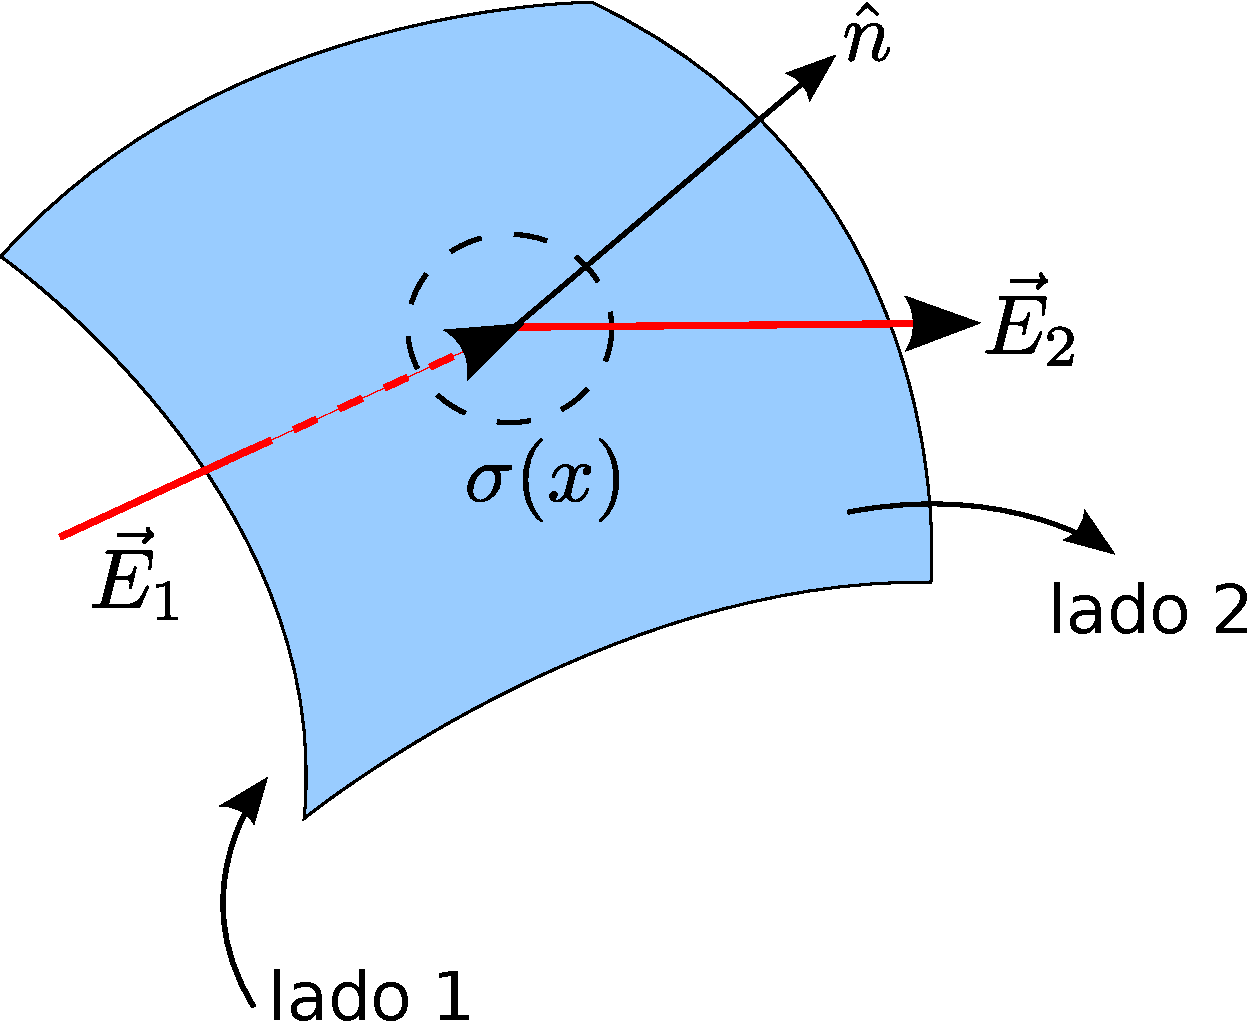
\psfig{file=fig/fig-superficie-frontera.pdf,height=6cm,angle=0}}
\caption{Condiciones de frontera para el campo el'ectrico.}
\label{DSCE1}
\end{figure}
Para estudiar las condiciones que el campo el'ectrico satisface en esta
interfase, aplicamos primero la ley de Gauss, a la superficie gaussiana de la
figura \ref{DSCE2}:
\begin{figure}[!h]
\centerline{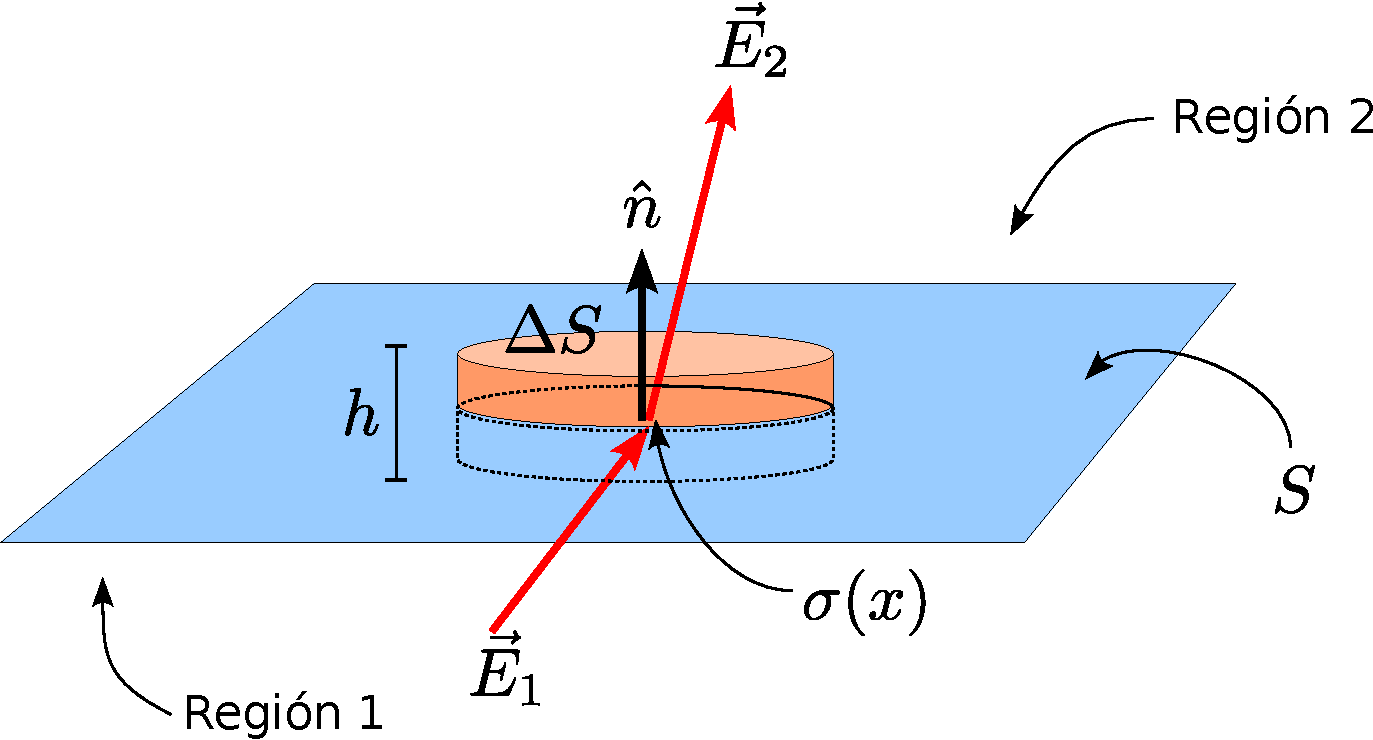
\psfig{file=fig/fig-condicion-borde-electrico-01.pdf,height=5cm,angle=0}}
\caption{Condici'on de frontera para la componente normal del campo el'ectrico.}
\label{DSCE2}
\end{figure}
\begin{eqnarray}
\oint_{S} \vec{E}\cdot d\vec{S}&=&\int_{S_1}
\vec{E}_1\cdot d\vec{S}+\int_{S_2} \vec{E}_2 \cdot d\vec{S}+\int_{S_3}
\vec{E}\cdot d\vec{S}\\
&=& -(\vec{E}_1\cdot\hat{n})\Delta S+(\vec{E}_2\cdot\hat{n})\Delta S+0\\
&=& \frac{\sigma S}{\varepsilon_0},
\end{eqnarray}
donde $\Delta S$ es una superficie, cuyo \textit{vector unitario $\hat{n}$ est'a dirigido
desde la cara $1$ a la cara $2$}, que contiene una densidad de carga
$\sigma(\vec{x})$ $\left[ C/m^2\right]  $, y los campos el'ectricos a
cada lado de la superficie son como se indica en la figura.

Por tanto, obtenemos
\begin{equation}\marginnote{Discontinuidad comp. normal}
\boxed{\vec{E}_2\cdot\hat{n}-\vec{E}_1\cdot\hat{n}=\frac{\sigma}
{\varepsilon_0}.}\label{saltoEn}
\end{equation}

Por otro lado, aplicando (\ref{ointE0}) a la curva de la figura \ref{DSCE3} obtenemos:
\begin{figure}[!h]
\centerline{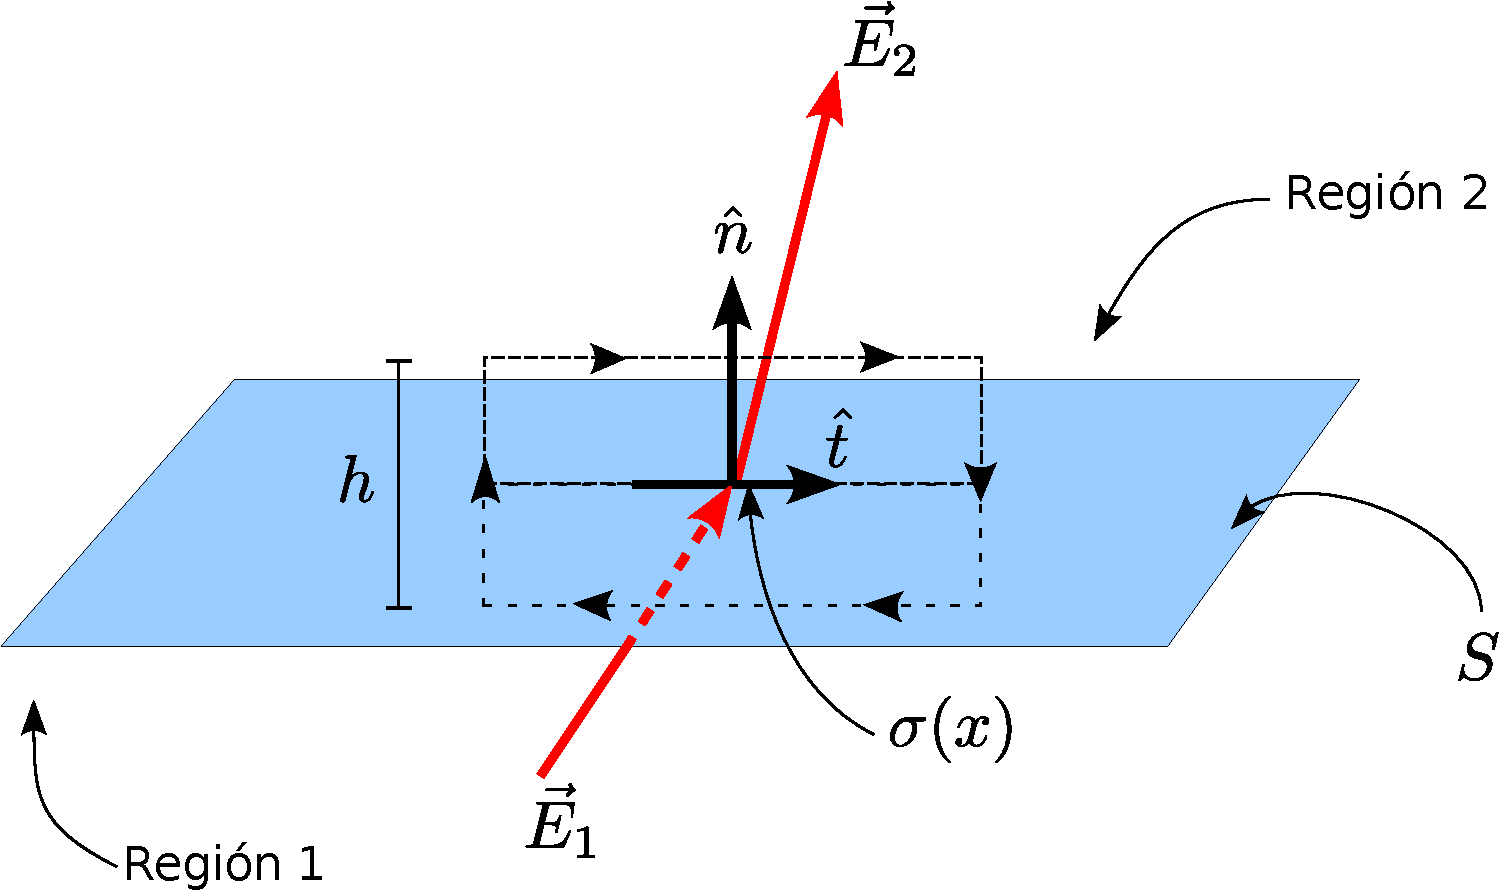
\psfig{file=fig/fig-condicion-borde-electrico-02.pdf,height=5cm,angle=0}}
\caption{Condici'on de frontera para la componente tangencial del campo el'ectrico.}
\label{DSCE3}
\end{figure}
\begin{eqnarray}
 \oint_{\cal C} \vec{E}\cdot d\vec{x}&=&\int_{{\cal C}_1} \vec{E}\cdot
d\vec{x}+\int_{{\cal C}_2} \vec{E}\cdot d\vec{x}+\int_{{\cal C}_3}
\vec{E}\cdot d\vec{x}+\int_{{\cal C}_4} \vec{E}\cdot d\vec{x} \\
&=& -(\vec{E}_1\cdot\hat{t})\ell +(\vec{E}_2\cdot\hat{t})\ell +0+0 \\
&=& 0.
\end{eqnarray}
De aqu'i encontramos que
\begin{equation}\marginnote{Continuidad comp. tangencial}
 \boxed{\vec{E}_2\cdot\hat{t}=\vec{E}_1\cdot\hat{t}.} \label{Etconst}
\end{equation}
Ya que la direcci'on del vector $\hat{t}$ es arbitraria (pero siempre
tangencial a la superficie $S$), la condici'on (\ref{Etconst}) implica que
 \textit{las componentes tangenciales (2 componentes linealmente idependientes) del campo el'ectrico permanecen inalteradas
al cruzar la superficie} $S$.

\subsection{Conductores}

Los \textbf{conductores} son materiales que, aunque est'en
el'ectricamente neutros a nivel macros\-c'o\-pi\-co, poseen
una enorme cantidad de electrones ``libres'' (es decir,  no ligados a
los 'atomos, y que pueden moverse a trav'es del conductor tan pronto como
exista un campo el'ectrico que induzca su movimiento)
aptos para conducir la electricidad. La carga de estos electrones es
neutralizada (a escala macrosc'opica) por la de los protones que est'an en los n\'{u}cleos, que pueden considerarse fijos. Como ejemplo de conductores podemos mencionar a los metales y a los electrolitos (cambi'en conocidos como \textbf{soluciones i'onicas}).

Si un conductor es cargado, o est'a en presencia de cargas externas, los electrones r'apidamente\footnote{Como veremos m'as adelante el \textit{tiempo de relajaci'on} es del orden de $\tau=\varepsilon/\sigma$ donde $\varepsilon$ es la \textit{constante diel'ectrica} del material y $\sigma$ su \textit{conductividad}. Por ejemplo, para el cobre $\tau\approx 10^{-19}$s.} se desplazan hasta una situaci'on de \textit{equilibrio}, es decir, un \textit{estado estacionario}. En este
estado el campo el'ectrico (macrosc'opico) en el interior del conductor debe anularse ya que de otro modo la fuerza sobre ellos ser'ia no nula, induciendo
movimiento. Por tanto, en situaci'on estacionaria $\vec{E}=\vec{0}$ en el
\textit{interior} de los conductores. Como consecuencia de la ley de Gauss, la
densidad de carga en el interior del conductor se anula cuando 'este
alcanza su estado estacionario. En otras palabras, \textit{un conductor en estado estacionario distribuye su carga neta sobre su superficie}.

Aplicando las condiciones de borde (\ref{saltoEn}) y (\ref{Etconst}) a la
interfase del conductor, y tomando en cuenta que en este caso
$\vec{E}_1=\vec{0}$, encontramos que \textit{en cada punto de la superficie (exterior) del conductor}
\begin{equation}\marginnote{Campo fuera de conductor}
 \vec{E}_2(x)=\frac{\sigma(x)}{\varepsilon_0}\hat{n}(x), \label{Econd}
\end{equation}
es decir, que el campo el'ectrico es normal a la superficie, y proporcional a la densidad de carga en cada punto de 'esta. El potencial el'ectrico, por otro lado, es necesariamente constante tanto dentro del conductor como sobre su superficie.

\subsection{Sobre (dis)continuidad de los campos}
 Idealmente, al menos cl'asica y macrosc'opicamente, la distribuci'on de carga descrita por la densidad volum'etrica $\rho(\vec{x})$ debiese ser una funci'on \textit{finita y continua} en todo punto. Como consecuencia, el campo el'ectrico y el potencial ser'ian, de acuerdo a (\ref{cerho}) y (\ref{perho}), tambi'en funciones finitas y cont'inuas. Sin embargo, com'unmente es \textit{conveniente} idealizar la distribuci'on de cargas, considerando que 'esta est'a limitada a una superficie bidimensional (es decir, de secci'on transversal despreciable). Este caso corresponde a considerar una densidad volum'etrica $\rho$ singular (discontinua y divergente)\footnote{Por ejemplo, la densidad volum'etrica correspondiente a una carga distribuida en todo el plano $xy$, con densidad superficial de carga $\sigma(x,y)$ puede escribirse como $\rho(x,y,z)=\sigma(x,y)\delta(z)$.}. En este caso, el campo el'ectrico poseer'a, en general, \textit{discontinuidades} en la superficie donde $\rho$ es singular, tal como analizamos en la secci'on \ref{secCBE}, pero ser'a \textit{finito en todo punto}. El potencial, por otro lado, ser'a una \textit{funci'on continua y diferenciable por tramos}. En resumen, para distribuciones de carga singulares que incluyan distribuciones superficiales de carga, el potencial puede siempre considerarse como una funci'on continua, el campo el'ectrico (proporcional a las derivadas del potencial) puede tener discontinuidades, mientras que las segundas derivadas del potencial (proporcionales a las primeras derivadas del campo el'ectrico y, a trav'es de la ecuaci'on de Poisson (\ref{poisson}), ligadas a la densidad volum'etrica de carga) pueden poseer regiones (superficies) singulares. En el caso de que la distribuci'on de carga se modele incluyendo cargas puntuales o l'ineas de carga, el potencial ya no ser'a finito en todo punto.


\section{Soluci'on de la ecuaci'on de Laplace}
\subsection{Coordenadas Esf'ericas}
Una soluci'on general (finita sobre el eje $z$) de la ecuaci'on de Laplace en coordenadas esf'ericas puede escribirse como:
\begin{equation}
  \boxed{\phi(r,\theta,\varphi) = \sum_{l=0}^\infty\sum_{m=-l}^l\left[
  A_{lm}  r^l + B_{lm}  r^{-(l+1)}\right]  Y_{lm}(\theta,\varphi),}
  \label{est31b}
\end{equation}
donde $A_{lm}$ y $B_{lm}$ son coeficientes constantes. Note que estos
coeficientes son en general complejos.

Si, como caso particular, el potencial tiene simetr'ia axial, es decir no
depende de la coordenada $\varphi$, entonces la expansi'on se reduce a
\begin{eqnarray}
  \phi(r,\theta) &=& \sum_{l=0}^\infty\left[
  A_{l0}  r^l + B_{l0}  r^{-(l+1)}\right]  Y_{l0}(\theta,\varphi) \\
&=&\sum_{l=0}^\infty\left[  A_{l0}  r^l + B_{l0}
r^{-(l+1)}\right]\sqrt{\frac{2l+1}{4\pi}}\,P_l(\cos\theta) ,
\end{eqnarray}
o, equivalentemente,
\begin{equation}\label{phiaxial}
\boxed{\phi(r,\theta)=\sum_{l=0}^\infty\left[  a_l\,  r^l +
\frac{b_l}{r^{l+1}}\right]\,P_l(\cos\theta),}
\end{equation}
donde $a_l$ y $b_l$ son nuevos coeficientes reales constantes.

\subsubsection{Ejemplo: Esfera conductora en un campo el'ectrico externo}\label{sec:esfcond}

Consideramos una esfera conductora de radio $R$ ubicada en un campo externo inicial homog'eneo $\vec{E}_0$. Elegimos los ejes coordenados de modo que el origen coincida con el centro de la esfera y el eje $z$ con la direcci'on del campo externo, es decir, $\vec{E}_0=E_0\hat{z}$.

Luego de ubicar la esfera en el campo externo, las cargas libres en ella se reacomodan r'apidamente. En la situaci'on estacionaria final el campo el'ectrico en el interior de la esfera es nulo, es decir, $\vec{E}=0$ para $r<R$. Como consecuencia directa $\phi=\text{cte.}$ para $r<R$. Podemos elegir esta constante igual a cero, de modo que
\begin{equation}
\phi(r,\theta)=0, \qquad r<R.
\end{equation}
Por otro lado, de acuerdo a (\ref{Econd}) el campo el'ectrico en la superficie externa del conductor es radial, y proporcional a la densidad de carga $\sigma(\theta,\varphi)$. Debido que el sistema es sim'etrico bajo rotaciones en torno a la direcci'on de $\vec{E}$, tendremos que $\phi=\phi(r,\theta)$ y $\sigma=\sigma(\theta)$. Finalmente, fuera de la esfera el potencial satisface la ec. de Laplace, por lo que 'este debe tener la forma general (\ref{phiaxial}). Por lo tanto, para determinar el potencial en todo punto basta determinar los coeficientes (constantes) $a_l$ y $b_l$.

Una condici'on necesaria es que asimpt'oticamente, es decir, para $r\to\infty$, el campo debe tender al campo externo inicial ya que los efectos de las cargas inducidas en la esfera ser'an cada vez menores en puntos cada vez m'as alejados, es decir, $\vec{E}\to\vec{E}_0 $. Esta condici'on es equivalente a 
\begin{equation}
\phi\to -E_0z+\alpha=-E_0r\cos\theta+\alpha .
\end{equation}
Aplicando esta condici'on a la expansi'on (\ref{phiaxial}) encontramos que necesariamente
\begin{equation}
a_0=\alpha, \qquad a_1=-E_0, \qquad a_2=a_3=\cdots =0,
\end{equation}
por lo que el potencial en todo punto se reduce a 
\begin{equation}
\phi(r,\theta)=\alpha -E_0 r\cos\theta +
\sum_{l=0}^\infty\frac{b_l}{r^{l+1}}P_l(\cos\theta), \qquad r\ge R.
\end{equation}
Como el potencial es una funci'on cont'inua, debemos tener que
\begin{equation}
\phi(R,\theta)=\alpha -E_0 R\cos\theta +
\sum_{l=0}^\infty\frac{b_l}{R^{l+1}}P_l(\cos\theta)=0, \qquad \forall \theta.
\end{equation}
De aqu'i, y ya que los polinomios de Legendre son funciones linealmente independientes, encontramos que necesariamente
\begin{equation}
\alpha+\frac{b_0}{R}=0, \qquad -E_0R+\frac{b_1}{R^2}=0, \qquad b_2=b_3=\cdots =0.
\end{equation}
Con esto, el potencial se reduce a
\begin{equation}\label{phialpha}
\phi(r,\theta)=\alpha -E_0 r\cos\theta -\alpha\frac{R}{r}+E_0 \frac{R^3}{r^2}\cos\theta. 
\end{equation}
La constante $\alpha$ es proporcional a la carga neta de la esfera. En efecto, usando (\ref{Econd}) podemos calcular la densidad superficial de carga en la esfera:
\begin{align}
\sigma(\theta) &= \varepsilon_0\, \vec{E}(R,\theta)\cdot\hat{r} \\
&= -\varepsilon_0 \frac{\partial\phi}{\partial r}(R,\theta) \\
&= -\varepsilon_0\left[-E_0\cos\theta+\frac{\alpha}{R}-2E_0\cos\theta\right]\\
&= \varepsilon_0\left[3E_0\cos\theta-\frac{\alpha}{R}\right].
\end{align}
La carga neta de la esfera es entonces
\begin{align}
Q &= \int_S\sigma(\theta)\,dS \\
&= 2\pi R^2 \int_0^\pi \sigma(\theta)\sen\theta\,d\theta \\
&= 2\pi \varepsilon_0R^2 \int_0^\pi \left[3E_0\cos\theta-\frac{\alpha}{R}\right] \sen\theta\,d\theta \\
&= 2\pi \varepsilon_0R^2 \left[ 0-\frac{2\alpha}{R}\right] \\
&= -4\pi \varepsilon_0R \alpha .
\end{align}
En otras palabras, 
\begin{equation}
\alpha=-\frac{Q}{4\pi \varepsilon_0}\frac{1}{R}.
\end{equation}
Con este resultado, el potencial (\ref{phialpha}) puede escribirse como 
\begin{equation}
\phi(r,\theta)=-\frac{Q}{4\pi\varepsilon_0 R}+\frac{Q}{4\pi\varepsilon_0}\frac{1}{r} -E_0 \left(1-\frac{R^3}{r^3}\right)r\cos\theta.
\end{equation}
Como vemos, los primeros dos t'erminos son independientes del campo externo y representan el potencial de la carga neta de la esfera (que hemos supuesto aislada). El tercer t'ermino es el campo externo inicial y por lo tanto el 'ultimo t'ermino describe el campo el'ectrico inducido producto de la polarizaci'on de la esfera conductora.
\begin{figure}[!h]
\centerline{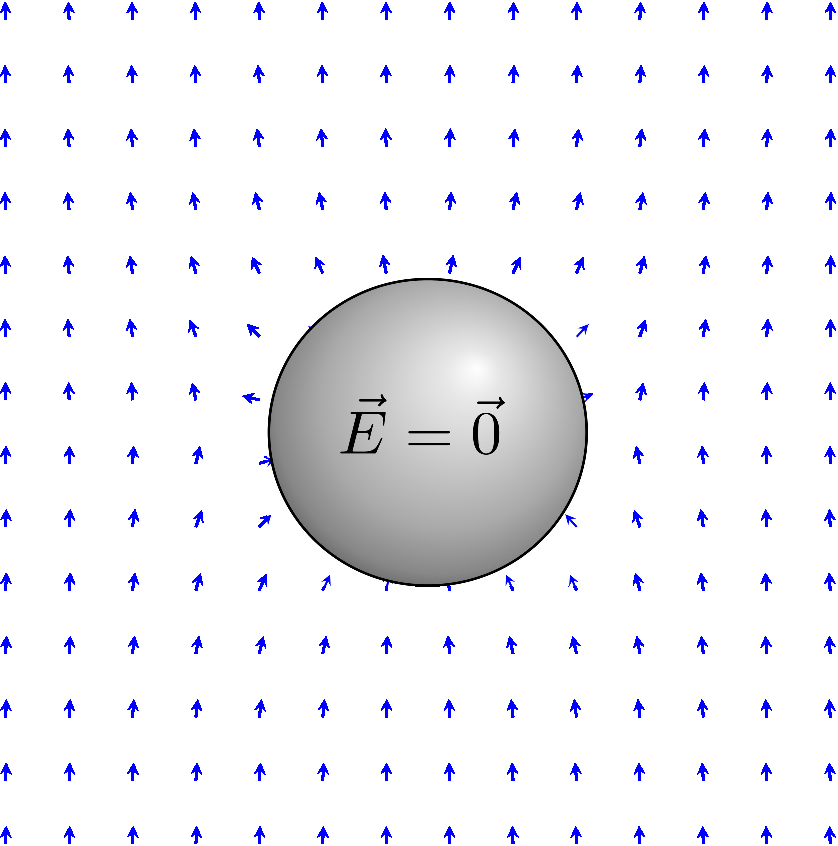
\psfig{file=fig/fig-esfera-conductora-campo-externo.pdf,height=5.5cm,angle=0}
\hspace{1cm}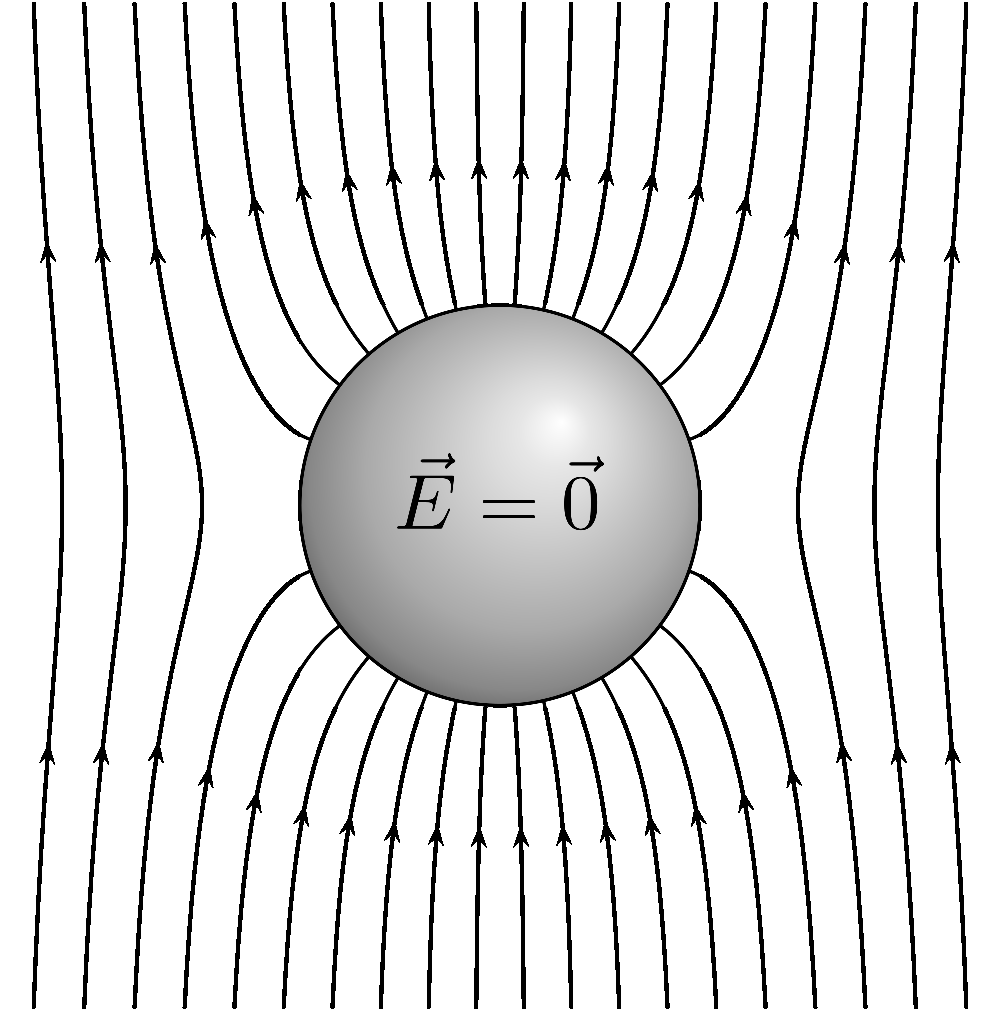
\psfig{file=fig/fig-esfera-conductora-campo-externo-2.pdf,height=5.5cm,angle=0}}
\caption{Campo el'ectrico de una esfera conductora neutra en un campo el'ectrico externo. El gr'afico de la izquierda (normalizado) fue creado usando \href{https://github.com/gfrubi/electrodinamica/blob/master/figuras-editables/fig-esfera-conductora-campo-externo-raw.py}{este script} Python. La figura de la derecha fue generada usando \href{http://commons.wikimedia.org/wiki/User:Geek3/VectorFieldPlot}{VectorFieldPlot}, a partir de \href{http://commons.wikimedia.org/wiki/File:VFPt_superconductor_ball_E-field.svg}{este} archivo original.}
\label{fig:ecce}
\end{figure}
El campo el'ectrico es entonces dado por
\begin{equation}
\vec{E}(r,\theta)=E_r\hat{r}+E_\theta\hat{\theta},
\end{equation}
con 
\begin{equation}
E_r=\frac{Q}{4\pi\varepsilon_0}\frac{1}{r^2}+E_0 \left(1+2\frac{R^3}{r^3}\right)\cos\theta, \qquad E_\theta=-E_0 \left(1-\frac{R^3}{r^3}\right)\sen\theta .
\end{equation}
En la figura \ref{fig:ecce} se muestra la forma de este campo, en el caso en que $Q=0$.


%\subsection{Coordenadas Cil'indricas}

%\subsection{Coordenadas Cartesianas}

 \section{Soluci'on de la ecuaci'on de Poisson} 
 \subsection{Soluci'on en t'erminos de Funciones de Green*}
 La ecuaci'on de Poisson \eqref{poisson} para el potencial es una \textit{EDP lineal el'iptica inhomog'enea}. Una forma de encontrar soluciones de este tipo de ecuaciones es usando el m'etodo de las \textit{funciones de Green}. En nuestro caso, se dice que $G(\vec{x},\vec{x}')$ es una funci'on de Green del operador Laplaciano si satisface
\begin{equation}\label{EDPG}
\nabla^2G(\vec{x}',\vec{x})=\delta(\vec{x}-\vec{x}').
\end{equation} 
Si se conoce una funci'on de Green entonces la soluci'on de la ecuaci'on de Poisson para el potencial en una regi'on $V$ puede expresarse de la forma siguiente:
\begin{align}
\phi(\vec{x}) &= -\frac{1}{\varepsilon_0}\int_VG(\vec{x},\vec{x}')\rho(\vec{x}')dV'+\oint_{\partial V}\left[\phi(\vec{x}')\vec\nabla' G(\vec{x},\vec{x}')-G(\vec{x},\vec{x}')\vec\nabla'\phi(\vec{x}')\right]\cdot d\vec{S}' \\
&=  -\frac{1}{\varepsilon_0}\int_VG(\vec{x},\vec{x}') \rho(\vec{x}')dV'+\oint_{\partial V}\left[\phi(\vec{x}')\frac{\partial G}{\partial n'}(\vec{x},\vec{x}')-G(\vec{x},\vec{x}')\frac{\partial\phi}{\partial n'}(\vec{x}')\right]dS'
\end{align}
Introduciendo el campo el'ectrico en el segundo t'ermino del lado derecho podemos escribir
\begin{equation}\label{solPoisson}
\phi(\vec{x})= -\frac{1}{\varepsilon_0}\int_VG(\vec{x},\vec{x}') \rho(\vec{x}')dV'+\oint_{\partial V}\left[\phi(\vec{x}')\frac{\partial G}{\partial n'}(\vec{x},\vec{x}')+G(\vec{x},\vec{x}')E_n(\vec{x}')\right]dS',
\end{equation}
donde $E_n:=\vec{E}\cdot\hat{n}$ es la componente del campo el'ectrico normal a la superficie $\partial V$ (con $\hat{n}$ orientado hacia el exterior del volumen $V$).

Por otro lado, la funci'on de Green no es 'unica. Si $G_1(\vec{x},\vec{x}')$ es una funci'on de Green entonces $G_2(\vec{x},\vec{x}')=G_1(\vec{x},\vec{x}')+H(\vec{x},\vec{x}')$ tambi'en lo ser'a si $H$ es una soluci'on del problema homog'eneo: en nuestro caso de la ecuaci'on de Laplace, $\nabla^2H(\vec{x},\vec{x}')=0$. Esta arbitrariedad en la definici'on de la funci'on de Green es de hecho una ventaja, puesto que en general no se tiene informaci'on \textit{simult'anea} del potencial y la componente normal del campo en la frontera $\partial V$. Por esto, es conveniente elegir una funci'on de Green de modo que los t'erminos del lado derecho de \eqref{solPoisson} puedan efectivamente ser evaluados. Por ejemplo, si se conoce el potencial\footnote{condici'on de borde tipo Dirichlet.} en $\partial V$ (t'ipicamente, en situaciones donde $\partial V$ coincide con la superfice de conductores conectados a bater'ias suministrando una diferencia de potencial conocida) entonces es conveniente usar una \textit{funci'on de Green que se anule en la frontera}, $G(\vec{x},\vec{x}')=0$, $\forall$ $\vec{x}'\in\partial V$. En este caso, la soluci'on se reduce a
\begin{equation}\label{solPoissonDirichlet}
\phi(\vec{x})= -\frac{1}{\varepsilon_0}\int_VG(\vec{x},\vec{x}') \rho(\vec{x}')dV'+\oint_{\partial V}\phi(\vec{x}')\frac{\partial G}{\partial n'}(\vec{x},\vec{x}')dS',
\end{equation}
 Por otro lado, si se conoce la componente normal del campo en la frontera\footnote{condici'on de borde tipo Neumann.} (por ejemplo, en situaciones donde se dispone de informaci'on sobre la densidad de carga superficial en $\partial V$) entonces parece conveniente usar una funci'on de Green tal que su derivada normal sobre la frontera sea nula. Lamentablemente, esta condici'on \textit{no es posible de implementar} ya que necesariamente\footnote{Use el teorema de Gauss sobre la integral de volumen de \eqref{EDPG} para verificar esto!.} debe cumplirse que
\begin{equation}\label{intGn}
\oint_{\partial V}\frac{\partial G}{\partial n'}dS'=1.
\end{equation}
Una condici'on un poco menos restrictiva, y factible de implementar consistentemente, es imponer que la derivada normal de la funci'on de Green sea \textit{constante en la frontera}. Entonces, \eqref{intGn} requiere que
\begin{equation}
\frac{\partial G}{\partial n'}(\vec{x},\vec{x}')=\frac{1}{S}, \qquad \vec{x}'\in\partial V,
\end{equation}
donde $S$ es el 'area total de la frontera, $S:=\oint_{\partial V} dS$. En este caso, la soluci'on para el potencial adopta la forma
\begin{equation}
\phi(\vec{x})= \left\langle\phi\right\rangle_S-\frac{1}{\varepsilon_0}\int_VG(\vec{x},\vec{x}') \rho(\vec{x}')dV'+\oint_{\partial V}G(\vec{x},\vec{x}')E_n(\vec{x}')dS',
\end{equation}
donde
\begin{equation}
\left\langle\phi\right\rangle_S:=\frac{1}{S}\oint_{\partial V}\phi(\vec{x}')\,dS'
\end{equation}
es el \textit{valor promedio del potencial sobre} $\partial V$.

Finalmente, la funci'on de Green m'as conocida del operador Laplaciano es dada por
\begin{equation}
G(\vec{x}-\vec{x}')=-\frac{1}{4\pi}\frac{1}{|\vec{x}-\vec{x}'|}.
\end{equation}
Esta funci'on de Green particular posee las propiedades adicionales de ser sim'etrica bajo rotaciones respecto al punto $\vec{x}'$, depender s'olo de la diferencia $\vec{x}-\vec{x}'$ y de anularse en el infinito (para todo valor finito de $\vec{x}'$). Debido a estas propiedades est'a directamente relacionada con la soluci'on de la ecuaci'on de Poisson en el caso en que la regi'on $V$ cubre todo el espacio y se asume que el campo el'ectrico se anula en el infinito\footnote{m'as r'apido que $1/r$, es decir, tal que $\lim_{|x|\to\infty}|\vec{E}|r=0$.}, de modo que el potencial se reduce a
\begin{equation}
\phi(\vec{x})= \left\langle\phi\right\rangle_\infty+\frac{1}{4\pi\varepsilon_0}\int_V\frac{\rho(\vec{x}')}{|\vec{x}-\vec{x}'|}dV'.
\end{equation}

\subsection{Unicidad de la soluci'on}\label{sec:uniP}
A continuaci'on probaremos que \textit{la soluci'on de la ecuaci'on de Poisson es 'unica} (salvo una constante aditiva), en una regi'on $V$, para valores dados del potencial \textit{o de la componente normal del campo} en la frontera\footnote{Condiciones de borde tipo Dirichlet o tipo Neumann, respectivamente.} $\partial V$. Para esto, asumimos que existen dos soluciones distintas de \eqref{poisson} en $V$, $\phi_1(\vec{x})$ y $\phi_1(\vec{x})$, que \textit{satisfacen las mismas condiciones de borde}, es decir, su valor es conocido en $\partial V$ o bien su derivada normal es conocida en esta frontera.

Definimos la diferencia $U(\vec{x}):=\phi_1(\vec{x})-\phi_2(\vec{x})$ que ser'a entonces una soluci'on de la ecuaci'on de Laplace, $\nabla^2U=0$. En la frontera $\partial V$ esta funci'on satisface $U=0$ o bien ${\partial U}/{\partial n}=0$, ya que asumimos que $\phi_1$ y $\phi_2$ satisfacen las mismas condiciones de borde (tipo Dirichlet, o bien tipo Neumann). Usamos ahora la identidad\footnote{Esta identidad es un caso particular de la as'i llamada \textit{primera identidad de Green}.}
\begin{equation}
 \int_V\left[\left|\vec\nabla U\right|^2+U\nabla^2U\right]  \,dV
 \equiv\oint_SU\frac{\partial U}{\partial n}\,dS,
 \end{equation}
que puede ser verificada f'acilmente usando el teorema de Gauss. En nuestro caso, dada la EDP y las condiciones de borde que $U$ satisface, la identidad implica que
\begin{equation}
 \int_V\left|\vec\nabla U\right|^2dV=0.
\end{equation}
Como consecuencia la funci'on $U$ debe ser \textit{constante}\footnote{En principio, esto ser'ia v'alido excepto (a lo sumo) en un conjunto de medida cero. Sin embargo, esta posibilidad queda descartada si el potencial es una funci'on continua.}, por lo que las dos soluciones $\phi_1$ y $\phi_2$ s'olo pueden diferir por una constante, representando la misma soluci'on f'isica\footnote{M'as a'un, para condiciones de borde tipo Dirichlet, esta constante es necesariamente nula.}.

Es importante notar que este resultado implica que, en general, es inconsistente intentar encontrar una soluci'on de la ecuaci'on de Poisson \textit{imponiendo simult'aneamente el valor del potencial y de su derivada normal en la frontera}.

Note que los teoremas anteriores implican que el campo el'ectrost'atico en una regi'on $V$ queda totalmente determinado por la densidad de carga en el interior del volumen $V$, y por las condiciones de borde en la frontera $\partial V$. Una de las m'ultiples consecuencias de este hecho es que el campo al interior de un volumen de forma arbitraria, cuya frontera es mantenida a un potencial fijo (por ejemplo, por medio de un conductor puesto ``a tierra'') es \textit{independiente de la distribuci'on de cargas en el exterior}. De esta forma, es posible aislar una regi'on de las influencias el'ectricas externas (``jaula de Faraday'').


\section{M'etodo de las im'agenes}
Como vimos la secci'on \ref{sec:uniP}, la soluci'on de la ecuaci'on de Poisson, que determina el potencial electrost'atico y por lo tanto tambi'en el campo el'ectrico, es 'unica dadas las condiciones de borde apropiadas. Debido a esto, si
obtenemos, \textit{por cualquier m'etodo}, una soluci'on que respete las condiciones de
borde dadas, 'esta es \textit{la} soluci'on del problema. El \textit{m'etodo de
las im'agenes} suministra un procedimiento para encontrar una soluci'on en
casos donde el sistema contiene conductores (perfectos) a potencial constante
(t'ipicamente, ``puestos a tierra'') y la geometr'ia de los conductores y las
cargas es simple. Para ello, se introducen \textit{cargas ficticias} en
posiciones apropiadas tales que el campo creado por el sistema de cargas reales
+ ficticias satisface las condiciones de borde.

En otras palabras, el m'etodo de las im'agenes se basa en el hecho que la
soluci'on para el campo el'ectrico en una regi'on finita $V$ con una
distribuci'on de carga conocida y potenciales dados en su superficie
$\partial V$ pueden ser los mismos (\underline{en $V$}) que los campos generados por la
misma distribuci'on de carga en $V$ \textit{y por otra distribuci'on de carga
diferente fuera de $V$}. Por esto, para solucionar el problema ``real'', en el
que la distribuci'on de carga en $V$ y los potenciales en $\partial V$ son conocidos, se
puede considerar el problema ``ficticio'' de encontrar las cargas ``imagenes''
fuera de $V$ tales que la distribuci'on de cargas total (reales e im'agenes)
satisfaga las condiciones de contorno en $\partial V$. Los campos as'i encontrados son
soluci'on del problema original, dentro (pero \underline{no} fuera) de $V$. Como veremos, el m'etodo de las im'agenes b'asicamente provee un m'etodo heur'istico para encontrar la funci'on de Green apropiada a las condiciones de borde de un cierto problema f'isico.



\subsection{Conductor plano}
\begin{figure}[!h]
\centerline{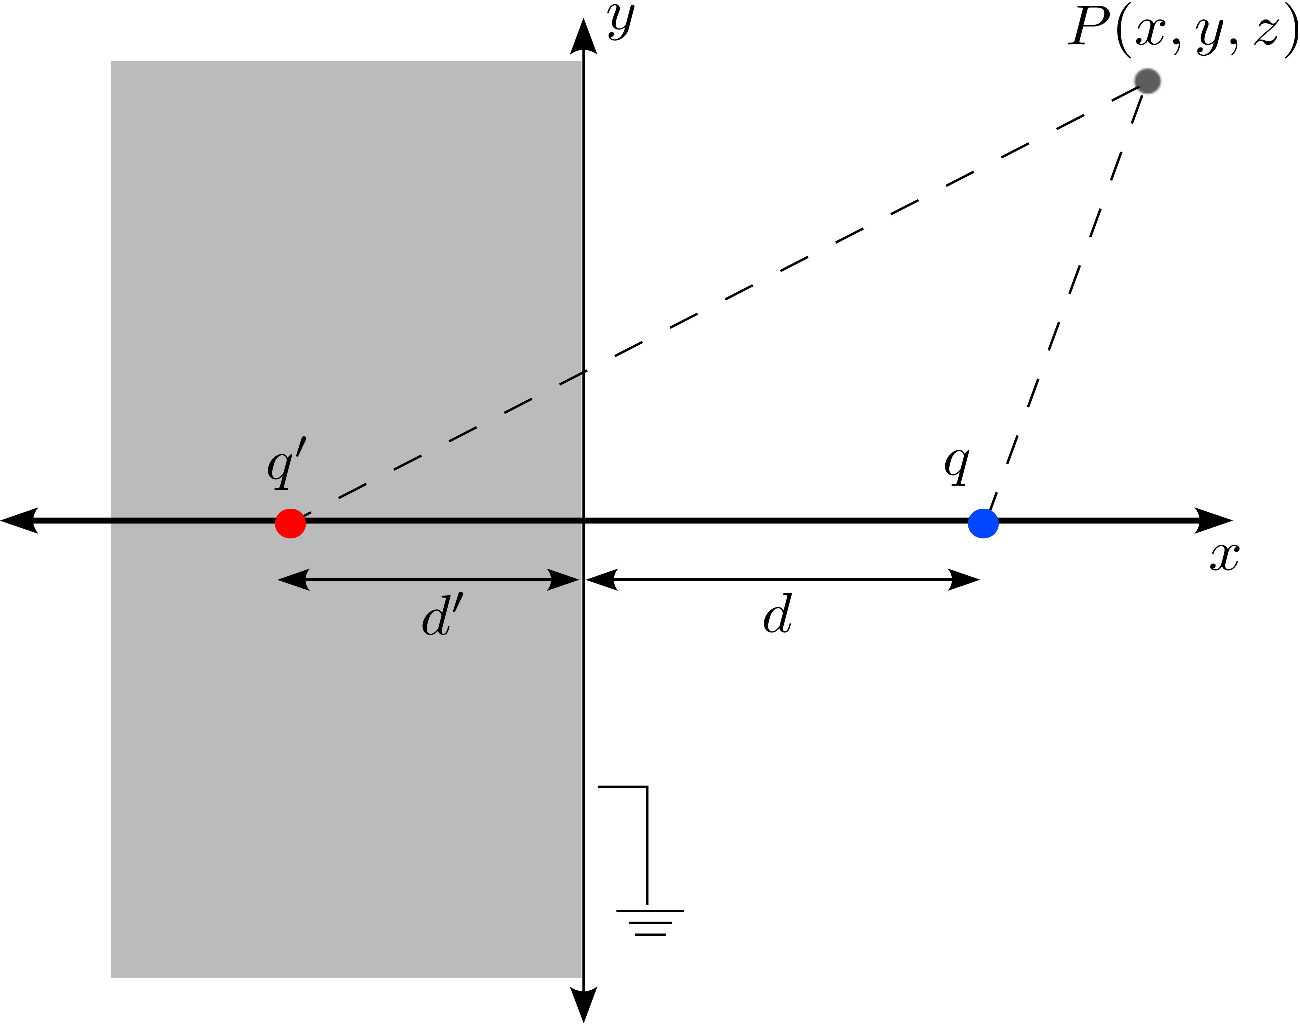
\psfig{file=fig/fig-carga-imagen-01.pdf,height=6cm,angle=0}}
\caption{Conductor plano, carga real $q$ e imagen $q'$.}
\label{ci01}
\end{figure}
Consideremos la situaci'on donde una carga puntual $q$ se encuentra a una distancia $d$ de un plano conductor (infinito) ``puesto a tierra'' (de modo que su potencial es igual al potencial en el infinito, elegido como $\phi_\infty=0$). Eligiendo los ejes coordenados como lo indica la figura \ref{ci01}, tendremos que en la situaci'on estacionaria $\phi=0$ para $x\le 0$. Usando el m'etodo de las im'agenes resolvemos el problema equivalente obtenido al reemplazar el plano conductor por una carga ficticia (imagen) $q'$ ubicada en la posici'on $x=-d'<0$. El potencial de la condiguraci'on de carga real m'as carga imagen es entonces
\begin{equation}
 \phi(x)=\frac{1}{4\pi\varepsilon_0}\left[\frac{q}{\sqrt{(x-d)^2+y^2+z^2}}+\frac
{q'}{\sqrt{(x+d')^2+y^2+z^2}}\right].
\end{equation}
La condici'on que $\phi=0$ sobre el plano, es decir, para todo punto con $x=0$,
se satisface s'olo si
\begin{equation}
 d'=d, \qquad q'=-q.
\end{equation}
Por lo tanto, la soluci'on para el potencial en todo punto con $x\ge 0$ es dada por
\begin{equation}
 \phi(x)=\frac{q}{4\pi\varepsilon_0}\left[\frac{1}{\sqrt{(x-d)^2+y^2+z^2}}-\frac
{1}{\sqrt{(x+d)^2+y^2+z^2}}\right], \qquad x\ge 0.
\end{equation}
\begin{center}
\begin{figure}[H]
\centerline{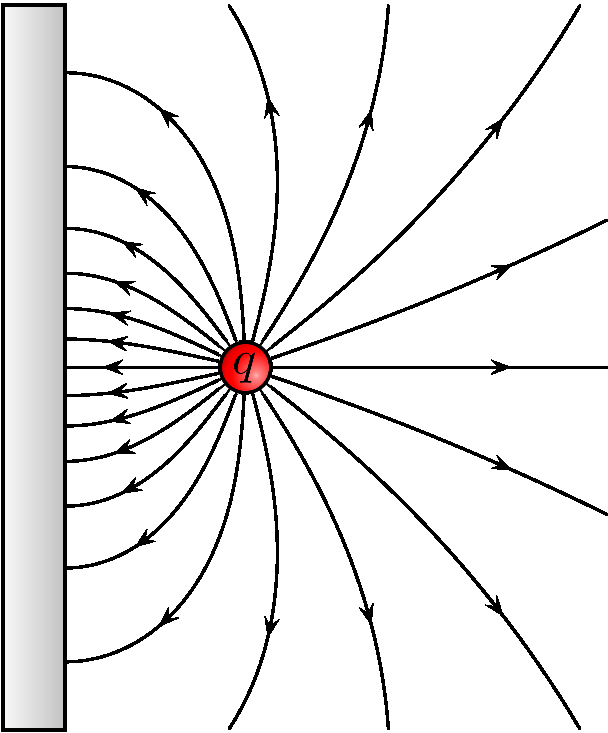
\psfig{file=fig/fig-metodo-imagen-plano-01.pdf,height=4.5cm,angle=0}
\hspace{2cm}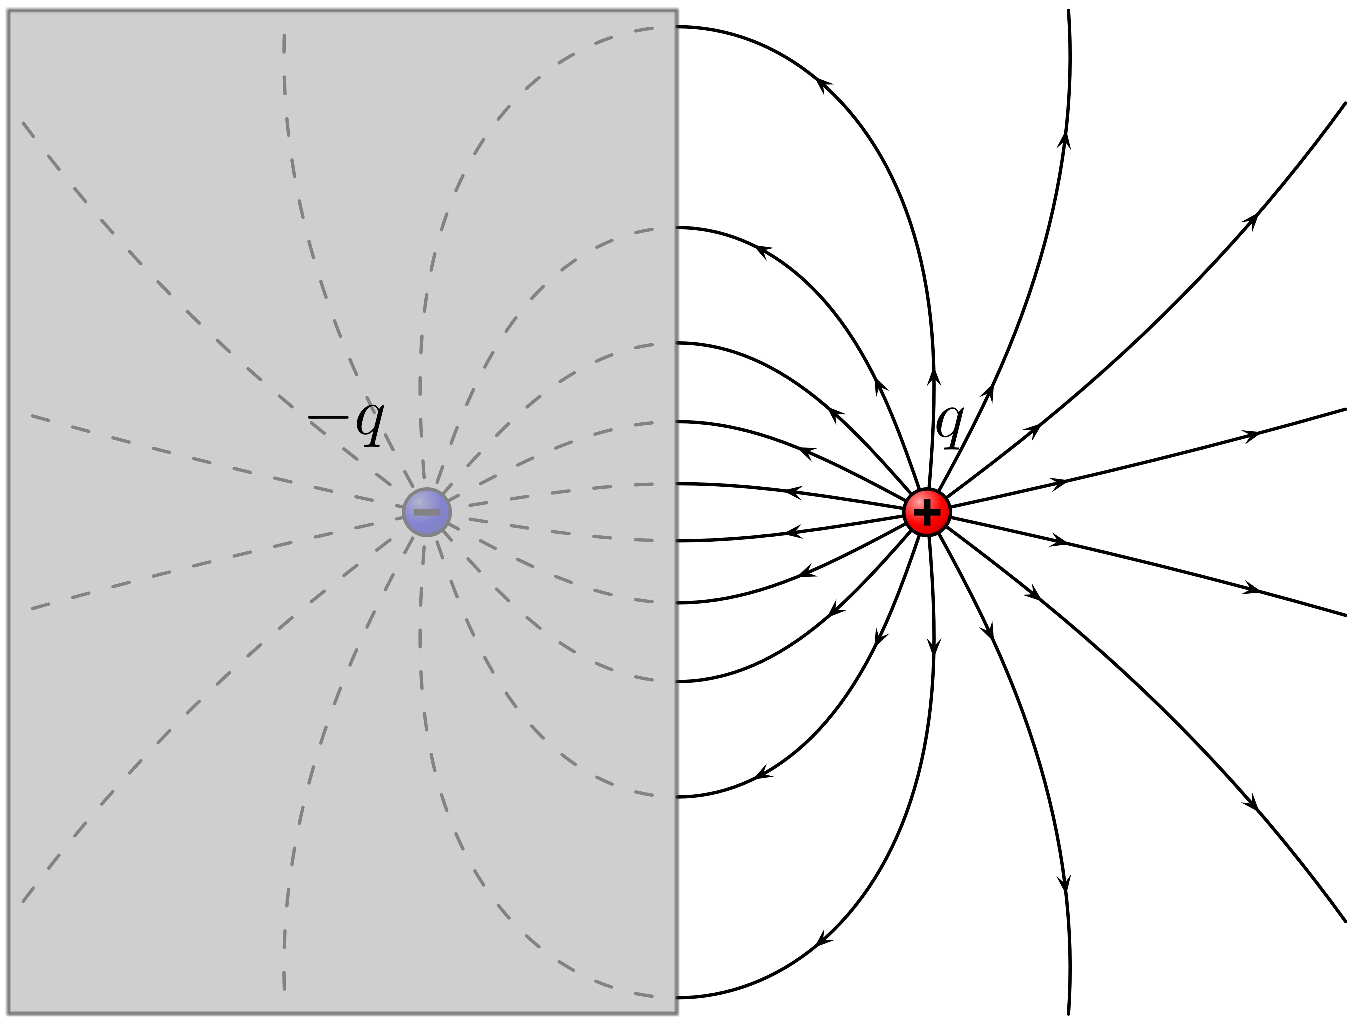
\psfig{file=fig/fig-metodo-imagen-plano-02.pdf,height=4.5cm,angle=0}}
\caption{Campo el'ectrico de plano conductor (puesto a Tierra) y carga puntual. 
Figuras adaptadas de  \href{http://commons.wikimedia.org/wiki/File:VFPt_image_charge_plane_horizontal.svg}{este} y \href{http://commons.wikimedia.org/wiki/File:VFPt_image_charge_plane.svg}{este} archivo original.}
\label{fig:pyc}
\end{figure}
\end{center}
La densidad de carga inducida en el conductor puede calcularse usando
\begin{equation}
 \sigma(y,z)=\varepsilon_0
\vec{E}\cdot\hat{n}=-\varepsilon_0\left.(\partial_x\phi)\right|_{x=0}
\end{equation}
que, luego de algo de 'algebra, resultar ser
\begin{equation}
 \sigma(y,z)=-\frac{q}{2\pi}\frac{d}{(d^2+y^2+z^2)^{3/2}}.
\end{equation}
Por otro lado, la fuerza que ejerce el plano sobre la carga puede ser calculada usando
\begin{equation}
\vec{F}_q=q\vec{E}',
\end{equation}
donde $\vec{E}'$ es el campo \textit{externo} que act'ua sobre $q$, es decir, el campo
determinado por el potencial
\begin{equation}
 \phi'(x)=-\frac{q}{4\pi\varepsilon_0}\frac{1}{\sqrt{(x+d)^2+y^2+z^2}},
\qquad x>0,
\end{equation}
evaluado en la posici'on en que se ubica la carga $q$, es decir,
\begin{eqnarray}
 \vec{F}_q&=&-q(\vec{\nabla}\phi')|_{\vec{x}=d\hat{x}} \\
&=&-\frac{q^2}{16\pi\varepsilon_0d^2}\,\hat{x}.
\end{eqnarray}
Note que esta fuerza es la misma que ejerce(r'ia) la carga imagen sobre la carga real.

\subsection{Conductor esf'erico}
\begin{figure}[!h]
\centerline{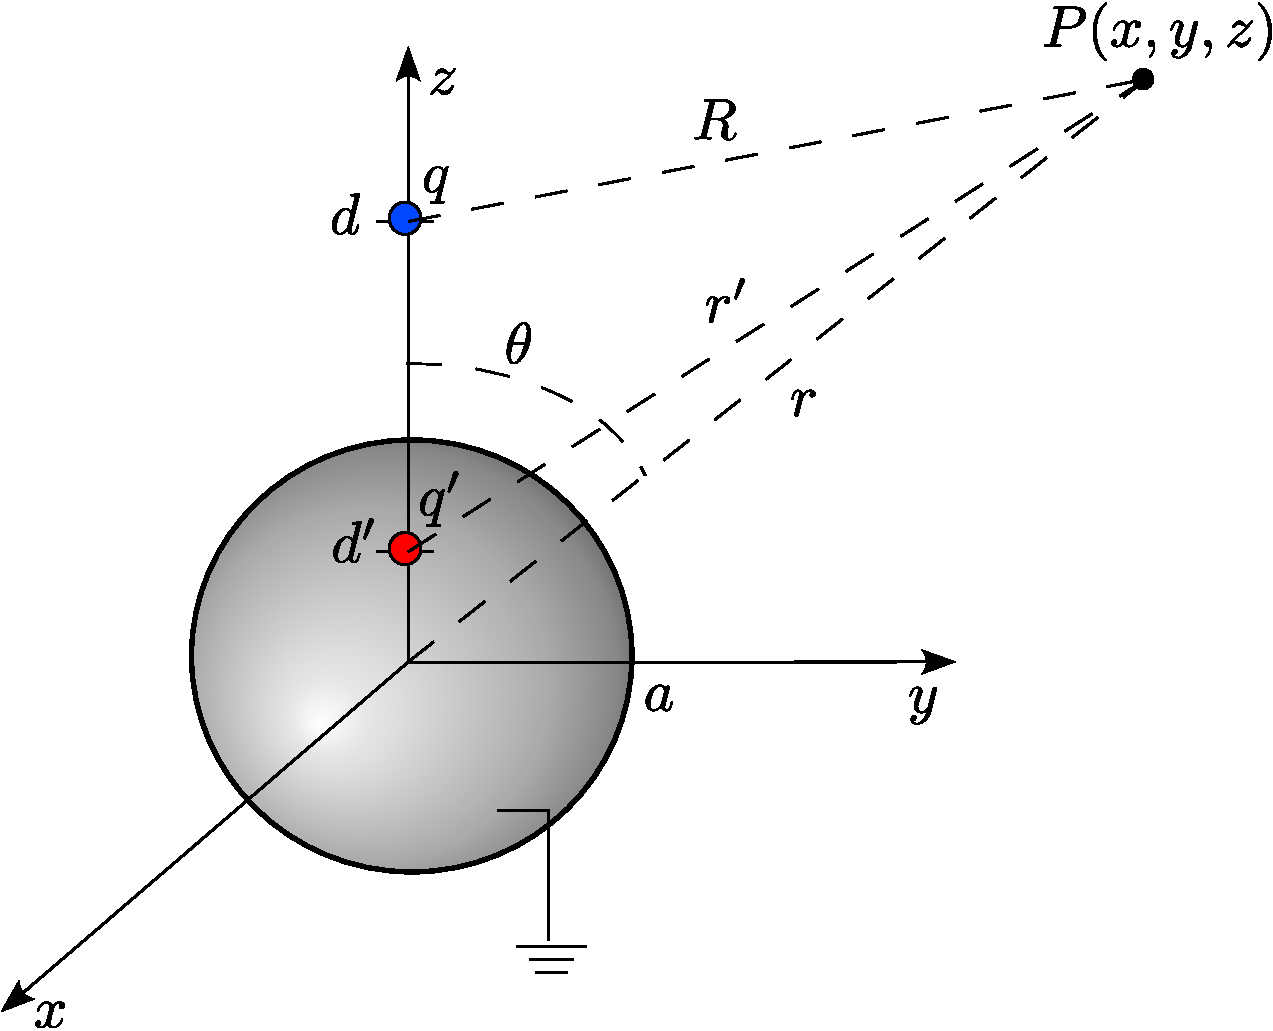
\psfig{file=fig/fig-carga-imagen-02.pdf,height=6cm,angle=0}}
\caption{Conductor esf'erico, carga real $q$ e imagen $q'$.}
\label{ci02}
\end{figure}
En este caso, consideramos el sistema formado por un conductor esf'erico, de radio $a$, ``puesto a tierra", de modo que su potencial $\phi=\phi_\infty\stackrel{!}{=}0$, y una carga puntual $q$ ubicada a una distancia $d$ del centro del conductor. El campo el'ectrico fuera del conductor es equivalente al campo producido por la carga real $q$ y una carga imagen de magnitud $q'$ ubicada dentro de la esfera, a una distancia $d'$ de su centro. 

En efecto, el potencial de la carga real y la carga imagen, de acuerdo a las posiciones indicadas en la figura \ref{ci02}, es dado por
\begin{equation}
 \phi(r,\theta)=\frac{1}{4\pi\varepsilon_0}\left[\frac{q}{\sqrt{
r^2+d^2-2dr\cos\theta } } +\frac{q'}{\sqrt{r^2+d'^2-2d'r\cos\theta}}\right]
\end{equation}
Puede verificarse r'apidamente que la condici'on que $\phi=0$ sobre la esfera, para todo punto con $r=a$, se satisface s'olo si
\begin{equation}
 d'=\frac{a^2}{d}, \qquad q'=-q\frac{a}{d}.
\end{equation}
Por lo tanto, la soluci'on para el potencial en todo punto exterior a la
esfera conductora es dada por
\begin{equation}\label{phice}
 \phi(r,\theta)=\frac{q}{4\pi\varepsilon_0}\left[\frac{1}{\sqrt{
r^2+d^2-2dr\cos\theta}}
-\frac{a}{\sqrt{a^4+r^2d^2-2a^2dr\cos\theta}}\right], \qquad r\ge a .
\end{equation}
\begin{center}
\begin{figure}[H]
\centerline{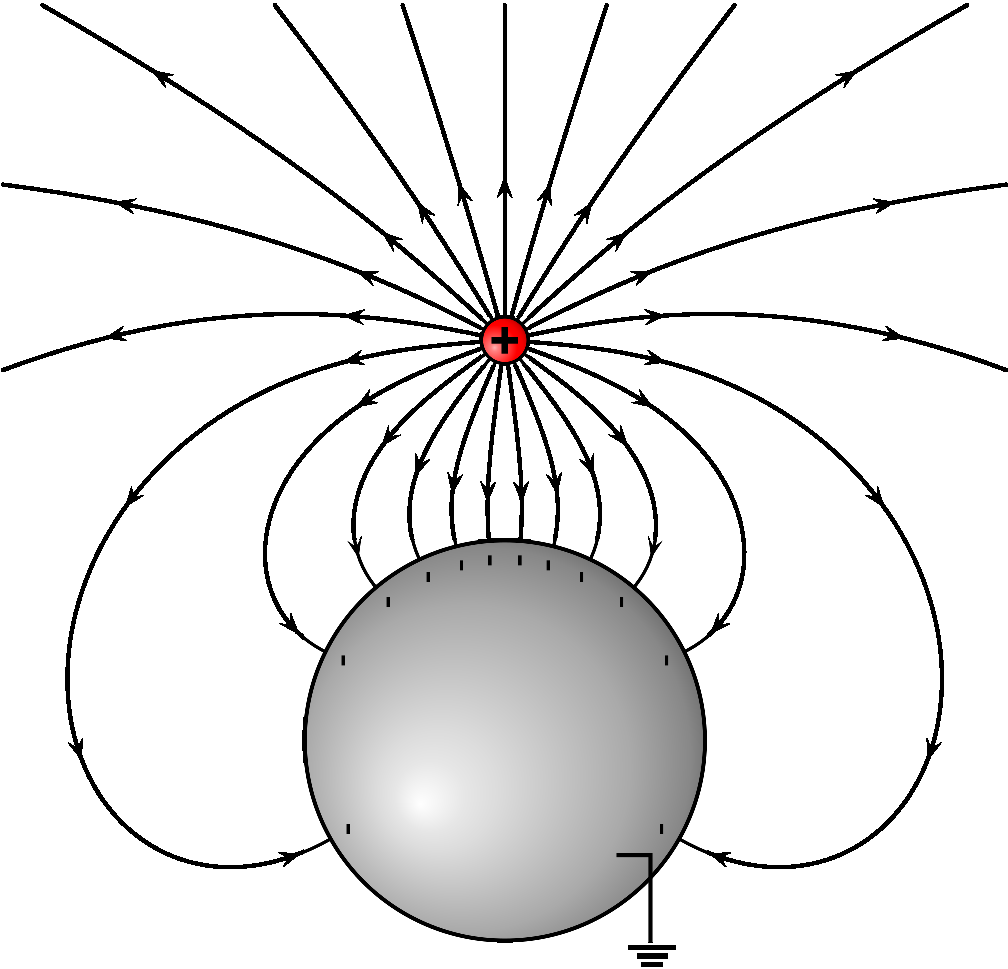
\psfig{file=fig/fig-metodo-imagen-esfera-01.pdf,height=5cm,angle=0}
\hspace{2cm}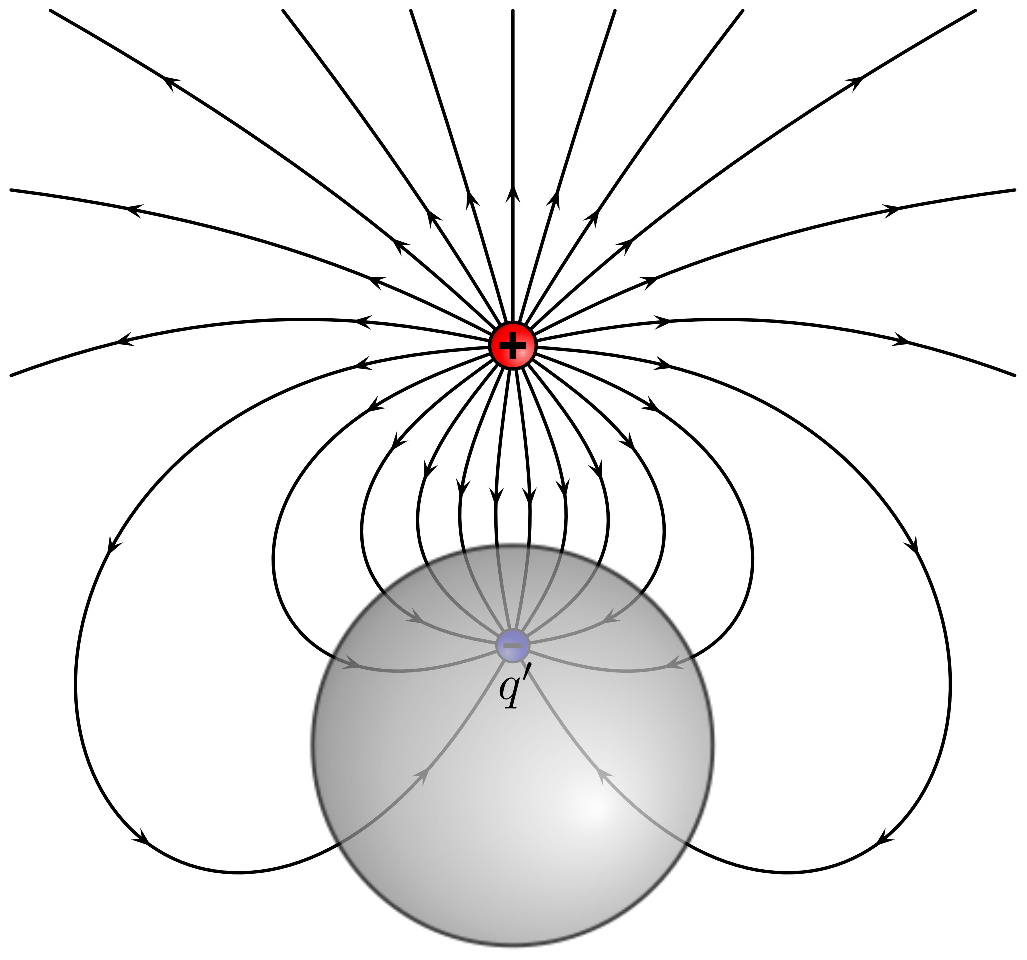
\psfig{file=fig/fig-metodo-imagen-esfera-02.pdf,height=5cm,angle=0}}
\caption{Campo el'ectrico de esfera conductora (puesta a Tierra) y carga puntual. 
Figuras adaptadas a partir de  \href{http://commons.wikimedia.org/wiki/File:VFPt_metal_ball_grounded.svg}{este} y \href{http://commons.wikimedia.org/wiki/File:VFPt_metal_ball_grounded_transparent.svg}{este} archivo original.}
\label{fig:eyc}
\end{figure}
\end{center}
La densidad de carga inducida en la esfera conductora puede calcularse usando
\begin{equation}\label{sce}
 \sigma(\theta)=\varepsilon_0\vec{E}\cdot\hat{n}
=-\varepsilon_0\left.(\partial_r\phi)\right|_{r=a}.
\end{equation}
Reemplazando (\ref{phice}) en (\ref{sce}) encontramos que
\begin{equation}
 \sigma(\theta)=-\frac{q}{4\pi}\frac{1}{ad}\frac{1-\frac{a^2}{d^2
}}{\left[1+\left(\frac{a}{d}\right)^2-2\left(\frac{a}{d}\right)\cos\theta\right]
^{3/2}}.
\end{equation}
La carga total inducida en la esfera es entonces
\begin{equation}
 Q_{\rm ind}=\oint\sigma\,dS=2\pi
a^2\int_0^\pi\sigma(\theta)\sin\theta\,d\theta=-q\frac{a}{d}.
\end{equation}
Note que necesariamente la esfera debe tener una carga neta (igual a la carga imagen) para que $\phi=0$ en su superficie.

Finalmente, la fuerza que la esfera ejerce sobre la carga es dada por
\begin{equation}
\vec{F}_q=-\frac{q^2}{4\pi\varepsilon_0}\frac{a}{d}\frac{1}{(d'-d)^2}\,
\hat{z}=-\frac { q^2 }{4\pi\varepsilon_0}\frac{ad}{(a^2-d^2)^2}\,\hat{z}.
\end{equation}

\subsection{Conductor Cil'indrico}
\begin{figure}[!h]
\centerline{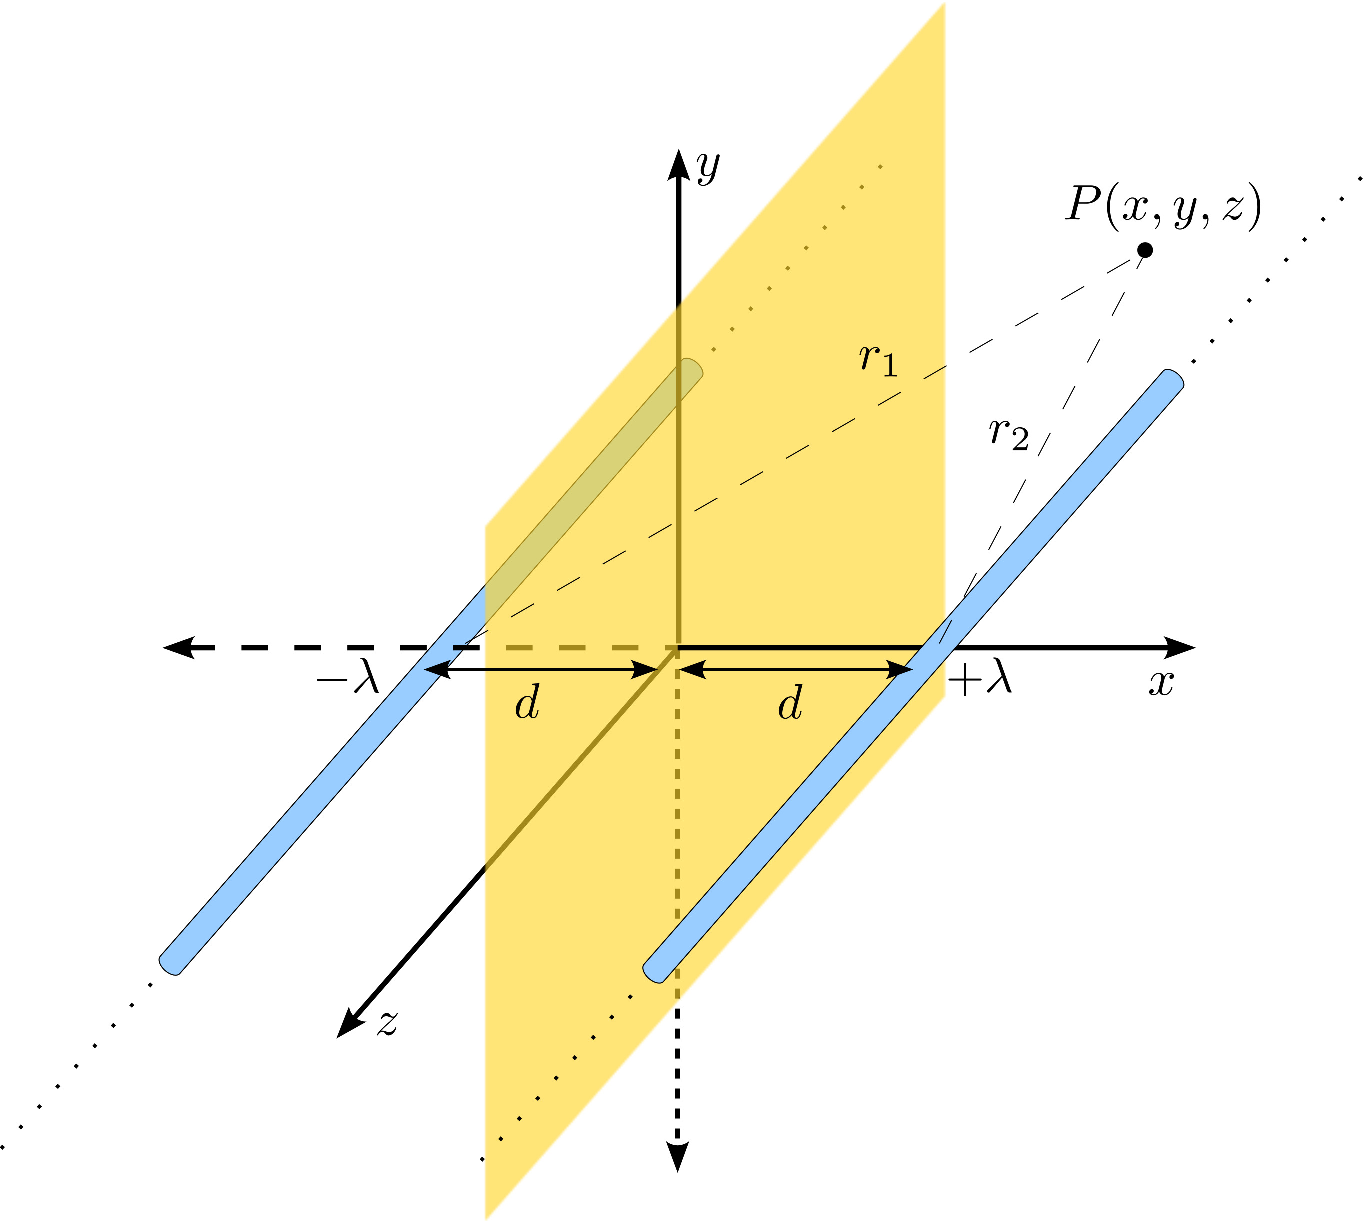
\psfig{file=fig/fig-metodo-imagenes-cilindros-01.pdf,height=6cm,angle=0}}
\caption{Conductor cil'indrico, l'ineas de densidad $\lambda$ y $-\lambda$.}
\label{ci03}
\end{figure}
Consideremos ahora el campo generado por dos l'ineas (infinitas) de carga, con
densidades lineales de carga $\lambda$ y $-\lambda$, situadas en $x=+d$ y
$x=-d$, respectivamente. Ver figura \ref{ci03}.

El potencial en un punto cualquiera fuera de las l'ineas de carga es dado por
\begin{equation}
 \phi(x,y)=\frac{\lambda}{2\pi\varepsilon_0}\ln\left(\frac{r_1}{r_2}
\right)=\frac{\lambda}{4\pi\varepsilon_0}\ln\left(\frac{r_1^2}{r_2^2}
\right)=\frac{\lambda}{4\pi\varepsilon_0}\ln\left(\frac{(x+d)^2+y^2}{
(x-d)^2+y^2}\right).
\end{equation}

Estudiemos la ubicaci'on de las superficies equipotenciales de esta
configuraci'on de cargas. Por simplicidad (de c'alculo), consideraremos las superficies con $\phi=\phi_0=\text{cte.}$, con
\begin{equation}
 \phi_0:=\frac{\lambda}{2\pi\varepsilon_0}\ln M, \label{phi0M}
\end{equation}
donde $M>0$ es una constante adimensional.  Con esto, las superficies $\phi=\phi_0$
corresponden a los puntos que satisfacen
\begin{equation}
 \frac{(x+d)^2+y^2}{(x-d)^2+y^2}=M^2. \label{equip1}
\end{equation}
Luego de un poco de 'algebra encontramos que, si $M\neq 1$, (\ref{equip1}) es
equivalente a
\begin{equation}
 \left[x-\frac{d(1+M^2)}{M^2-1}\right]^2+y^2=\frac{4M^2d^2}{(1-M^2)^2},
\end{equation}
que es la ecuaci'on de un cilindro (una circunsferencia en el plano $xy$),
centrado en las coordenadas $(x_{\rm c},y_c)$ y con radio $R$, dados por
\begin{equation}
 x_{\rm c}=\frac{d(1+M^2)}{M^2-1}, \qquad y_c=0, \qquad R=\frac{2Md}{|1-M^2|}.
\label{cilim}
\end{equation}
Vemos de aqu'i que (asumiendo $\lambda>0$) $x_{\rm c}<-d$ y $\phi_0<0$ si $M<1$,
mientras que $x_{\rm c}>d$ y $\phi_0>0$ si $M>1$.

Por otro lado, si $M=1$, entonces la superficie equipotencial es el plano
definido por $x=0$, es decir, el plano $yz$.

De estos resultados, vemos que las superficies equipotenciales del sistema de
cargas analizado son cil'indros centrados sobre el eje $x$ (a ambos lados del
plano $yz$ eje) y un plano a potencial nulo en $x=0$. Ver figura \ref{ci04}.
%
%Usando el m'etodo de las im'agenes podemos usar este resultado para encontrar el campo en el exterior de un cilindro conductor, en el caso en que fuera de 'este se ubica una  l'inea de carga paralela a su eje. Si 

Esta informaci'on puede ser usada, por ejemplo, para encontrar el campo
electrost'atico entre un plano y un cilindro, a una diferencia de potencial
dada $V$. Si el plano se encuentra en $x=0$, a potencial nulo y el cilindro, de
radio $R$, se ubicado en $x_{\rm c}>R$, entonces el campo puede ser determinado
considerando \textit{ambas l'ineas de carga como ficticias}. De las relaciones
(\ref{phi0M}), con $\phi_0=V$, y (\ref{cilim}) podemos entonces encontrar la
constante $M$, as'i como la posici'on, $d$, y magnitud $\lambda$ de las l'ineas
de cargas ficticias del problema equivalente, en funci'on de los datos $V$,
$x_0$ y $R$. Considerando que $V>0$, es decir, el potencial sobre el cilindro es mayor que sobre el plano y, de acuerdo a la figura \ref{ci04} el cil'indro est'a a la derecha del plano\footnote{Si $V<0$ la situaci'on es similar, luego de una reflexi'on respecto al plano $x=0$.} ($x_{\rm x}>0$). Luego de algo de 'algebra, obtenemos
\begin{equation}
 M=\frac{x_{\rm c}}{R}+\sqrt{\left(\frac{x_{\rm c}}{R}\right)^2-1}, \qquad
d=\frac{R(M^2-1)}{2M}, \qquad \lambda=\frac{2\pi\varepsilon_0V}{\ln M}.
\end{equation}
\begin{figure}[!h]
\centerline{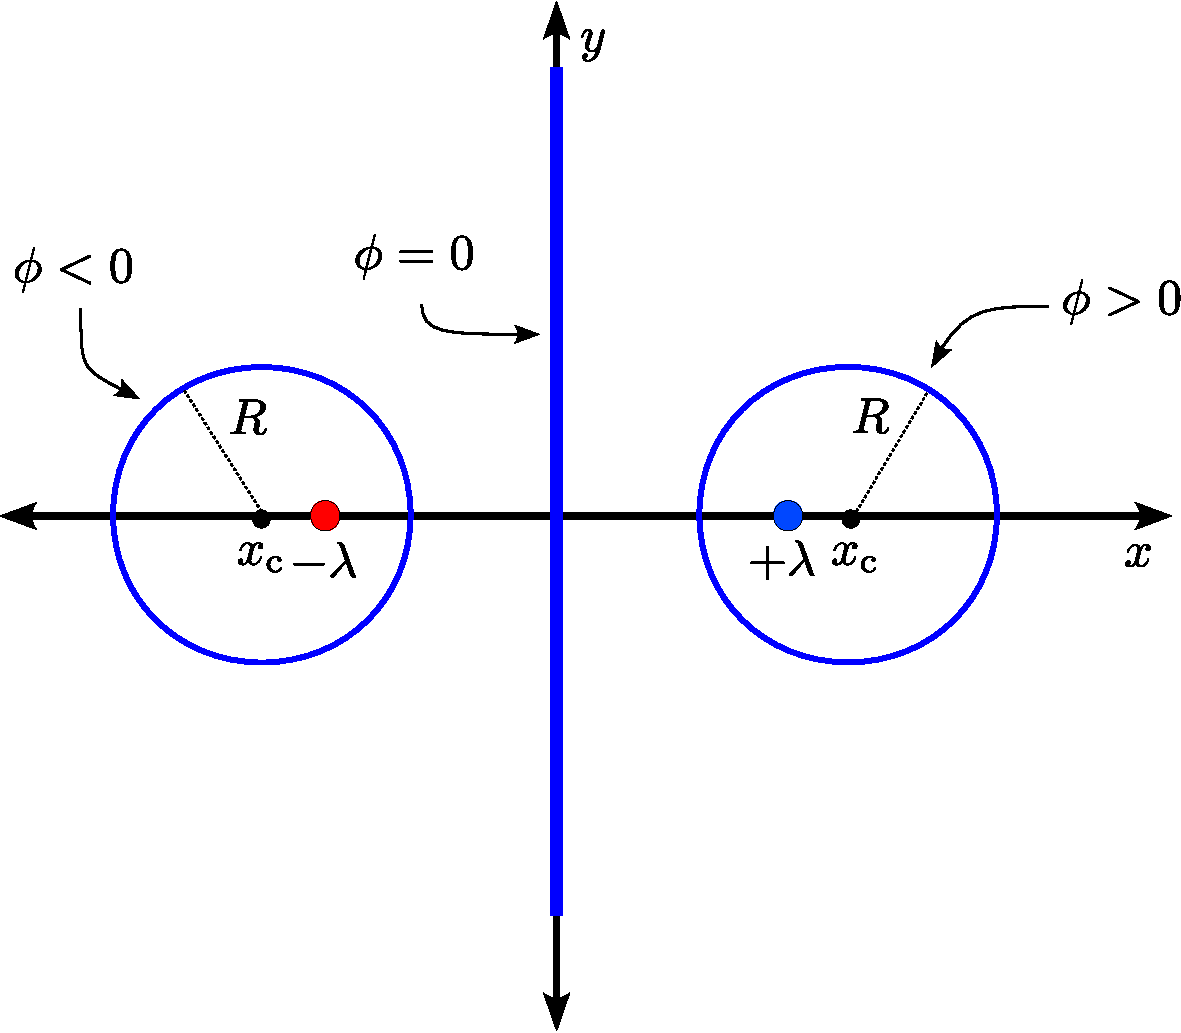
\psfig{file=fig/fig-metodo-imagenes-cilindros-02.pdf,height=6cm,angle=0}
\hspace{1cm}
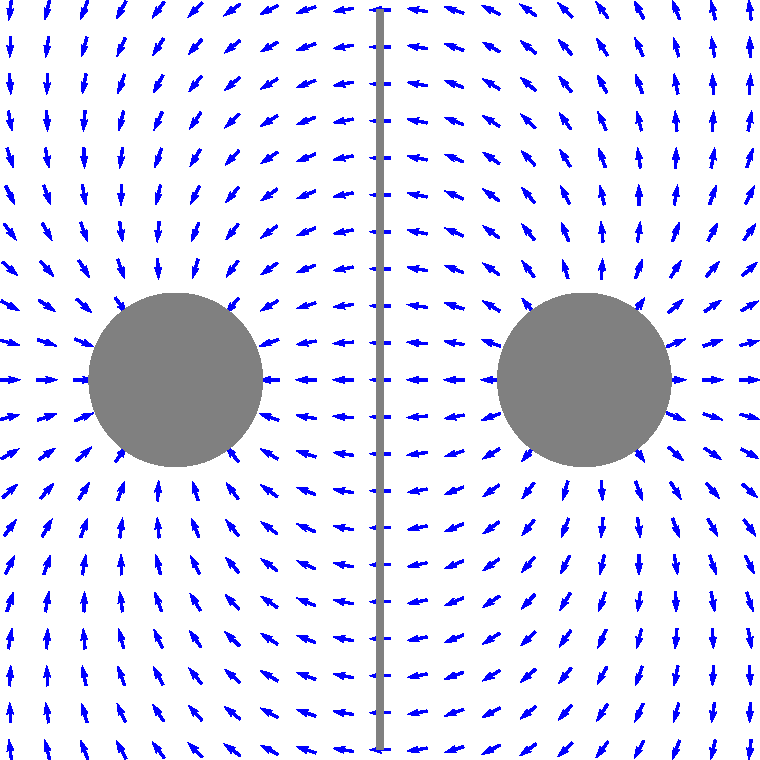
\psfig{file=fig/fig-metodo-imagenes-cilindros-03.pdf,height=6cm,angle=0}}
\caption{Superficies equipotenciales y l'ineas de campo. C'odigo Python de la figura de la derecha disponible \href{https://github.com/gfrubi/electrodinamica/blob/master/figuras-editables/fig-metodo-imagenes-cilindros-03.py}{aqu\'i}.}
\label{ci04}
\end{figure}

\section{Energ'ia potencial el'ectrica de cargas en un campo externo}
Como consecuencia de (\ref{E=nablaphi}), la fuerza electrost'atica es
\textit{conservativa}, pues puede derivarse de una energ'ia potencial (o,
equivalentemente, el trabajo es independiente de la trayectoria, ya que el campo
el'ectrico es irrotacional):
\begin{equation}
\boxed{F_i=qE_i=-q\partial_i\phi .}
\end{equation}
Definimos la \textbf{energ\'{\i}a potencial el'ectrica} de una carga $q$ ubicada en un punto $x$ con campo el'ectrico (externo) descrito por el potencial $\phi(x)$ por
\begin{equation}
\boxed{U(x):=q\phi(x),} \label{Uqphi}
\end{equation}
de modo
que
\begin{equation}
\boxed{F_i(x)=-(\partial_iU)(x) .}
\end{equation}
Como toda energ'ia potencial, la energ'ia potencial el'ectrica es una
cantidad bien definida salvo una constante aditiva arbitraria. Como
consecuencia, \textit{s'olo las diferencias de energ'ia potencial tienen
significado f'isico inambiguo} (pueden en principio ser medidas). Esta caracter'istica se
ilustra m'as claramente si consideramos el trabajo realizado por un campo
el'ectrico sobre una carga $q$ al desplazarse 'esta desde el punto $A$ hasta el
punto $B$:
\begin{equation}\label{WABDU}
W_{A\rightarrow B}=\int_A^B F_i\, dx_i=-\int_A^B
\partial_iU\,dx_i=-\left.U\right|_A^B=-\Delta U=-q\Delta\phi=-q(\phi_B-\phi_A).
\end{equation}

Como consecuencia, una part'icula cargada de masa $m$ y carga $q$ movi'endose en el campo el'ectrico externo descrito por el potencial $\phi$ tendr'a una energ'ia mec'anica $E=K+U=m\vec{v}^2/2+q\phi$, que ser'a constante si no existen otras fuerzas actuando, es decir,
\begin{equation}
E=\frac{1}{2}m\vec{v}^2+q\phi(x)=\text{cte.}
\end{equation}

Podemos generalizar la expresi'on \eqref{Uqphi} para el caso de una distribuci'on cont'inua de cargas \textit{de prueba}, en un campo \textit{externo}. En otras palabras, \textit{despreciamos el campo que las mismas cargas producen}. Por simple superposici'on encontramos que la energ'ia potencial de una distribuci'on de cargas descritas por la densidad $\rho(\vec{x})$ en un campo \textit{externo} $\phi(\vec{x})$ es dado por
\begin{equation} \label{Urhophiext}
U=\int \rho(\vec{x})\,\phi(\vec{x})\,dV.
\end{equation}

%\subsection{Ejemplo}
\section{Energ'ia potencial de un sistema de cargas}  \label{ed3_1}

\subsection{Energ'ia potencial de un conjunto de cargas puntuales}
\label{ed3_1_1}

Consideremos ahora el problema de determinar la \textit{energ'ia potencial total de un
conjunto de $N$ cargas puntuales}, pero \textit{ahora tomando en cuenta el campo que ellas mismas generan}. Cada carga $q^{(\alpha)}$ posee una energ'ia
potencial $U^{(\alpha\beta)}$ asociada al campo el'ectrico producido por cada una de las \textit{otras cargas}  $q^{(\beta)}$, con $\beta\ne \alpha$. Aqu'i $\alpha,\beta=1,\cdots, N$.

Adem'as, el potencial el'ectrico en el punto $\vec{x}$, generado por la carga $q^{(\beta)}$
ubicada en el punto $\vec{x}^{(\beta)}$, es dado por
\begin{equation}
\phi^{(\beta)}(\vec{x})=\frac{1}{4\pi\varepsilon_0}\,\frac{q^{(\beta)}}{|\vec{x}
-\vec{x}^{(\beta)}|} ,
\end{equation}
de modo que
\begin{equation} \label{eq3.1.3}
U^{(\alpha\beta)}=q^{(\alpha)}\,\phi^{(\beta)}(\vec{x}^{(\beta)})=\frac{1}{4\pi\varepsilon_0}\,\frac{q^{(\alpha)}\,q^{(\beta)}}{|\vec{x}^{(\alpha)}-\vec{x}^{(\beta)}|}.
\end{equation}
Vemos de (\ref{eq3.1.3}) que $U^{(\alpha\beta)}=U^{(\beta\alpha)}$, es decir, la energ'ia potencial de la carga $\alpha$-'esima debido al campo producido por la carga
$\beta$-'esima es igual a la energ'ia potencial de la $\beta$-'esima debido al campo
de la $\alpha$-'esima.

Adem'as,  $U^{(\alpha\beta)}\to 0$, cuando  $|\vec{x}^{(\alpha)}|\to\infty$
'o $|\vec{x}^{(\beta)}|\to\infty$. Entonces, de acuerdo a \eqref{WABDU}, \textit{podemos interpretar $U^{(\alpha\beta)}$ como la energ'ia (trabajo) que se necesita para traer la carga
$q^{(\alpha)}$ desde el infinito hasta la posici'on $\vec{x}^{(\alpha)}$, en el campo
el'ectrico producido por la carga $q^{(\beta)}$, fija en $\vec{x}^{(\beta)}$}, o
vicecersa.

Para calcular la energ'ia potencial el'ectrica total de un sistema de muchas cargas
puntuales, ``construimos'' el sistema, carga por carga, tray'endolas desde el
infinito (donde la interacci'on mutua es despreciable): Primero consideramos que la carga $q^{(1)}$ es transportada desde
el infinito hasta su posici'on final $\vec{x}^{(1)}$. Para esto no se requiere
trabajo alguno ya que no existe campo el'ectrico preexistente que act'ue sobre
esta carga. Como segundo paso, traemos la carga $q^{(2)}$ desde el infinito
hasta su posici'on final $\vec{x}^{(2)}$. Este proceso requiere una energ'ia
dada por $U^{(21)}$. En el siguiente paso, traemos $q^{(3)}$ desde el
infinito hasta $\vec{x}^{(3)}$, manteniendo fijas las cargas $q^{(1)}$ y
$q^{(2)}$. La energ'ia requerida para este paso es $U^{(31)}+U^{(32)}$. Hasta
el momento la energ'ia total requerida para formar el sistema de 3 cargas es
$U^{(21)}+U^{(31)}+U^{(32)}=U^{(12)}+U^{(13)}+U^{(23)}$. Continuando
este proceso encontramos que \textit{la energ'ia potencial el'ectrica total de un
sistema de $N$ cargas} $q^{(\alpha)}$, con posiciones $\vec{x}^{(\alpha)}$ es dado por
\begin{equation} \label{eq3.1.4}
U=\sum_{\alpha,\beta\,(\alpha>\beta)}^N U^{(\alpha\beta)}=\frac{1}{4\pi\varepsilon_0}\,
\sum_{\alpha,\beta\,(\alpha>\beta)}^N \frac{q^{(\alpha)}\,q^{(\beta)}}{|\vec{x}^{(\alpha)}-\vec{x}^{(\beta)}|}.
\end{equation}
Alternativamente, ya que $U^{(\alpha\beta)}=U^{(\beta\alpha)}$, podemos escribir
$U=({1}/{2})\sum_{\alpha,\beta\,(\alpha\ne \beta)}^N U^{(\alpha\beta)}$, de modo que
\begin{equation} \label{eq3.1.5}\marginnote{Energ'ia sist. cargas puntuales}
\boxed{U=\frac{1}{8\pi\varepsilon_0}\,
\sum_{\alpha,\beta\,(\alpha\ne \beta)}^N \frac{q^{(\alpha)}\,q^{(\beta)}}{|\vec{x}^{(\alpha)}-\vec{x}^{(\beta)}|}.}
\end{equation}
En t'erminos del \textit{potencial el'ectrost'atico total en el punto $\vec{x}^{(\alpha)}$
debido a todas las otras cargas} $q^{(\beta)}$ ($\beta\ne \alpha$),
\begin{equation}
\phi'(\vec{x}^{(\alpha)})=\frac{1}{4\pi\varepsilon_0}\,
\sum_{\beta\,(\beta\ne \alpha)}^N \frac{q^{(\beta)}}{|\vec{x}^{(\alpha)}-\vec{x}^{(\beta)}|},
\end{equation}
tenemos que
\begin{equation}\label{Wqphi}
\boxed{U= \frac{1}{2}\,\sum_{\alpha=1}^N q^{(\alpha)}\,\phi'(\vec{x}^{(\alpha)}).}
\end{equation}

\subsection{Energ'ia potencial de una distribuci'on continua de cargas} \label{ed3_1_2}
En el caso de una \textit{distribuci'on continua} de carga descrita por una densidad de carga $\rho(\vec{x})$, requerimos una expresi'on similar a la encontrada en la secci'on anterior para cargas puntuales. En el l'imite continuo, esperamos poder reemplazar $q^{(\alpha)}\to dq=\rho(\vec{x})\,dV$. Por otro lado, podr'iamos esperar que el potencial $\phi'(x^{(\alpha)})$ tienda simplemente al potencial de la distribuci'on continua de carga, evaluado en el punto $\vec{x}$, es decir, $\phi'(x^{(\alpha)})\to\phi(\vec{x})$, ya que no tiene sentido hacer distinci'on, en el caso de una distribuci'on continua, entre el campo $\phi'$ (es decir, el potencial producido por las cargas del sistema localizadas en puntos $\vec{x}'\neq\vec{x}$) y el simplemente el potencial $\phi(\vec{x})$. 

De este modo, obtenemos
\begin{equation}\marginnote{Energ'ia de dist. continua}
\boxed{U= \frac{1}{2}\,\int\rho(\vec{x})\,\phi(\vec{x})\,dV.} \label{Urhophi}
\end{equation}

Es importante entender la diferencia entre \eqref{Urhophiext} y \eqref{Urhophi}. La primera expresi'on representa la energ'ia potencial de una distribuci'on de cargas \textit{en un campo externo}, \textit{despreciando el campo que ellas mismas producen} (cargas ``de prueba"), mientras que la segunda representa \textit{la energ'ia potencial total contenida en un sistema de cargas debido su propio campo}. En otras palabras, los potenciales involucrados en \eqref{Urhophiext} y \eqref{Urhophi} son de naturaleza distinta: en la primera expresi'on representa el potencial externo, y en la segunda el potencial generado por las propias cargas. \textit{S'olo en el segundo caso el potencial est'a relacionado con la densidad por medio de la ecuaci'on de Poisson}.

Adem'as, si bien al aplicar la integral \eqref{Urhophi} al caso de distribuciones continuas y finitas de carga se obtienen resultados finitos, al intentar aplicarla al caso de una carga \textit{puntual} (o conjuntos de cargas puntuales) se encuentra un resultado \textit{divergente}. Esto, sin embargo, es usualmente interpretado asumiendo que  una carga puntual es una \textit{idealizaci'on}: el l'imite en que el tama\~no de la carga es nulo.
En la pr'actica, consideraremos a \eqref{Urhophi} como la expresi'on general para la energ'ia de una distribuci'on general de cargas, mientras que para un conjunto de cargas puntuales usaremos (\ref{eq3.1.5}) o, alternativamente, (\ref{Wqphi}).

\subsubsection{Derivaci'on alternativa}
Podemos derivar la expresi'on \eqref{Urhophi} considerando el proceso de ``construcci'on'' del sistema en que la densidad es aumentada paulatinamente desde 0 hasta $\rho(\vec{x})$. Si en un instante dado la densidad es, en cada punto, una fracci'on $\lambda$ ($0\le\lambda\le 0$) de la densidad total, es decir, si la densidad es $\lambda\rho(\vec{x})$, entonces el potencial generado por esta densidad es $\phi_\lambda(\vec{x})=\lambda\phi(\vec{x})$, ya que las la ecuaci'on que determina el potencial a partir de la densidad de carga (la ec. de Poisson (\ref{poisson})) es lineal. Entonces el trabajo necesario para aumentar la fracci'on de carga desde $\lambda$ hasta $\lambda+d\lambda$ es el trabajo necesario para transportar las cargas $dq=d\lambda\,\rho(\vec{x})dV$ desde el infinito hasta sus posiciones finales, en el campo $\phi_\lambda(\vec{x})$. Por lo tanto, el trabajo total requerido para aumentar la densidad de carga en una fracci'on $d\lambda$ es dado por:
\begin{align}
dW &= \int_V dq\,\phi_\lambda(\vec{x}) \\
&= \int_V \left[d\lambda\,\rho(\vec{x})\,dV\right]\left[\lambda\phi(\vec{x})\right] \\
&= \lambda d\lambda\,\int_V \rho(\vec{x})\phi(\vec{x}) \,dV . \label{dWlambda}
\end{align}
La energ'ia requerida en el proceso completo de ``construcci'on'' del sistema de cargas es entonces la suma de los trabajos de la forma (\ref{dWlambda}) desde $\lambda=0$ hasta $\lambda=1$, es decir,
\begin{equation}
U=\int_0^1dW,
\end{equation}
que lleva nuevamente a la expresi'on \eqref{Urhophi}.

\subsubsection{Energ'ia de un sistema de cargas formado por dos subsistemas}
Si tenemos un sistema de cargas que pueda ser separado en dos subsistemas, el primero con densidad de carga $\rho_1(x)$ que genera un potencial $\phi_1(x)$, y el segundo con densidad $\rho_2(x)$ y potencial $\phi_1(x)$, entonces 
\begin{equation}
\rho(x)=\rho_1(x)+\rho_2(x),
\end{equation}
ya suponemos que las regiones donde $\rho_2(x)$ y $\rho_2(x)$ son no nulas son disjuntas. Adem'as, en un punto cualquiera el potencial es dado por
\begin{equation}
\phi(x)=\phi_1(x)+\phi_2(x).
\end{equation}
Reemplazando estas expresiones en nuestro resultado general \eqref{Urhophi} encontramos que  la energ'ia del sistema completo puede ser escrita como
\begin{equation}
U=U_1+U_2+U_{\rm int}
\end{equation}
\begin{equation}
U_1= \frac{1}{2}\,\int\rho_1(\vec{x})\,\phi_1(\vec{x})\,dV ,\qquad U_2= \frac{1}{2}\,\int\rho_2(\vec{x})\,\phi_2(\vec{x})\,dV,
\end{equation}
\begin{align}
U_{\rm int} =& \int \rho_1(x)\phi_2(x)\,dV = \int \rho_2(x)\phi_1(x)\,dV.
\end{align}
La energ'ia $U_{\rm int}$ puede ser interpretada, de acuerdo a nuestro resultado \eqref{Urhophiext}, como la \textbf{energ'ia potencial de las cargas en el subsistema 1 debido al campo (externo) generado por el subsistema 2}, o bien como la \textbf{energ'ia potencial de las cargas en el subsistema 2 debido al campo (externo) generado por el subsistema 1}, o simplemente como la \textbf{energ'ia de interacci'on}.


\subsubsection{Energ'ia en funci'on del campo el'ectrico}

Podemos expresar la energ'ia \eqref{Urhophi} en t'erminos del campo el'ectrico,
usando la ley de Gauss (\ref{leygauss-dif}):
\begin{eqnarray}
U&=&\frac{1}{2}\,\int\rho(\vec{x})\,\phi(\vec{x})\,dV \\
&=&\frac{\varepsilon_0}{2}\,\int(\partial_i E_i)\,\phi\,dV\\
&=&\frac{\varepsilon_0}{2}\,\int\left[
\partial_i(E_i\phi)-E_i\partial_i\phi\right] dV\\
&=&\frac{\varepsilon_0}{2}\left[\oint
E_i\phi\,dS_i-\int E_i\partial_i\phi\, dV\right]\\
&=&\frac{\varepsilon_0}{2}\left[0+\int E_iE_i\, dV\right]\\
&=&\frac{\varepsilon_0}{2}\int \vec{E}^2\, dV.
\end{eqnarray}
En este c'alculo, hemos considerado que la integral de volumen se extiende sobre
todo el espacio, y que el campo el'ectrico se anula suficientemente r'apido en
el infinito, de forma tal que la integral de superficie es nula\footnote{La integral tiende a cero si $\phi$ decae m'as r'apido que $1/\sqrt{r}$ para $r\to\infty$. Esta condici'on es siempre satisfecha para distribuciones compactas de carga, donde se tiene de hecho que $\phi$ decae al menos como $1/r$.}. Con esto,
obtenemos
\begin{equation} \label{UuE}
\boxed{U=\int u_E(\vec{x})\,dV, \qquad u_E(\vec{x}):=\frac{\varepsilon_0}{2}\,
\vec{E}^2(\vec{x}) .}
\end{equation}
De esta forma, podemos calcular la energ'ia (potencial) electrost'atica de una
distribuci'on de carga como la integral de una \textit{densidad de energ'ia}
$u_E(\vec{x})$. Comparando (\ref{UuE}) con (\ref{eq3.1.5}) vemos que la
energ'ia potencial de un sistema de cargas puede interpretarse alternativamente
como la \textit{energ'ia almacenada en el campo el'ectrico} del sistema de
cargas, a trav'es de la densidad de energ'ia $u_E(\vec{x})$.

\subsubsection{Ejemplo}
\begin{figure}[!h]
\centerline{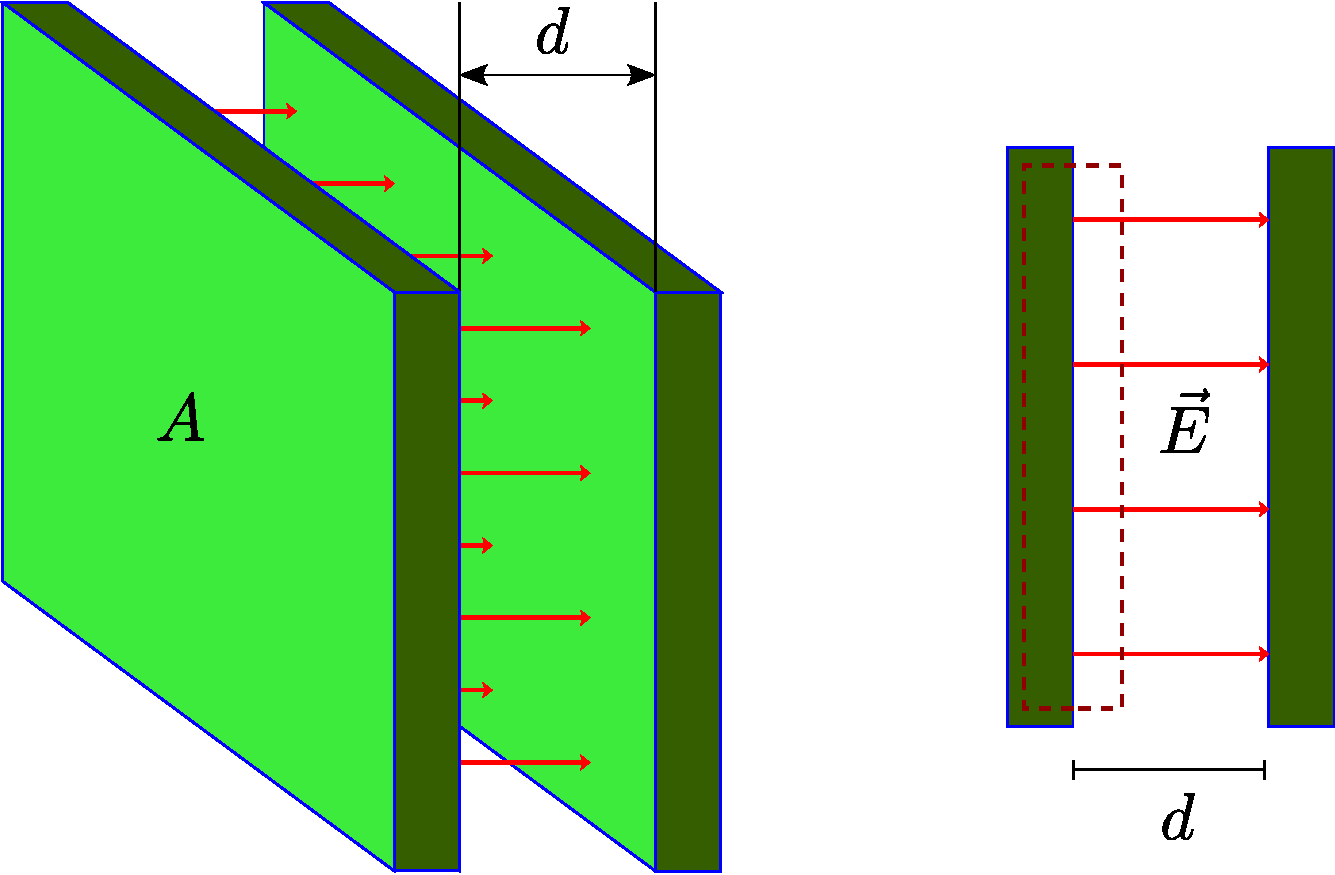
\psfig{file=fig/fig-condensador-01.pdf,height=4cm,
angle=0 } }
\caption{Energ'ia almacenada en un condensador de placas paralelas.}
\label{fig:cpp}
\end{figure}
Considere un condensador de placas paralelas, como se muestra en la figura \ref{fig:cpp}. Despreciando efectos de borde, es decir, considerando que dentro de la regi'on limitada por las placas en campo el'ectrico es homog'eneo y fuera de ella es nulo, y adem'as despreciando el espesor de las placas, podemos modelar la densidad de carga como
\begin{equation}
\rho(\vec{x})=\sigma\delta(x)-\sigma\delta(x-d), 
\end{equation}
para todo $(y,z)$ en la regi'on delimitada por las placas. 

El campo el'ectrico entre las placas (que puede obtenerse f'acilmente usando la ley de Gauss) es dado por
\begin{equation}
\vec{E}=\frac{\sigma}{\varepsilon_0}\hat{x}=E\hat{x}, \qquad 0<x<d,
\end{equation}
donde $\sigma$ es la densidad total de carga por unidad de superficie (en cada placa ubicada en $x=0$). Con esto, podemos evaluar la energ'ia \eqref{UuE} (el campo el'ectrico s'olo es no nulo entre las placas, que encierrar un volumen $V=Ad$):
\begin{equation} 
U=\int u_E(\vec{x})\,dV=\frac{\varepsilon_0}{2}\,
\vec{E}^2 V=\frac{\varepsilon_0}{2}\,
\vec{E}^2 Ad=\frac{\sigma^2}{2\varepsilon_0}Ad=\frac{Q^2}{2\varepsilon_0}\frac{d}{A} .
\end{equation}

Por otro lado, usando \eqref{phiintE} encontramos que el potencial entre las placas es de la forma
\begin{equation}
\phi(\vec{x})=\phi(0)-Ex=\phi(0)-\frac{\sigma}{\varepsilon_0}x, \qquad 0<x<d,
\end{equation}
con lo que podemos evaluar \eqref{Urhophi} (la densidad de carga s'olo es no nula sobre las placas), obteniendo
\begin{equation}
U=\frac{1}{2}\int\rho(x)\phi(x)\,dV=\frac{1}{2}\left[\sigma A\phi(0)-\sigma A\phi(d)\right]=\frac{\sigma^2 Ad}{2\varepsilon_0}=\frac{Q^2}{2\varepsilon_0}\frac{d}{A}.
\end{equation}
En t'erminos de la \textit{capacidad del condensador}, $C:=Q/\Delta V=\varepsilon_0 A/d$, tenemos
\begin{equation}
U=\frac{C(\Delta V)^2}{2}=\frac{Q^2}{2C}.
\end{equation}





\section{Expansi'on multipolar cartesiana}
\subsection{Expansi'on Multipolar}
\begin{figure}[!h]
\centerline{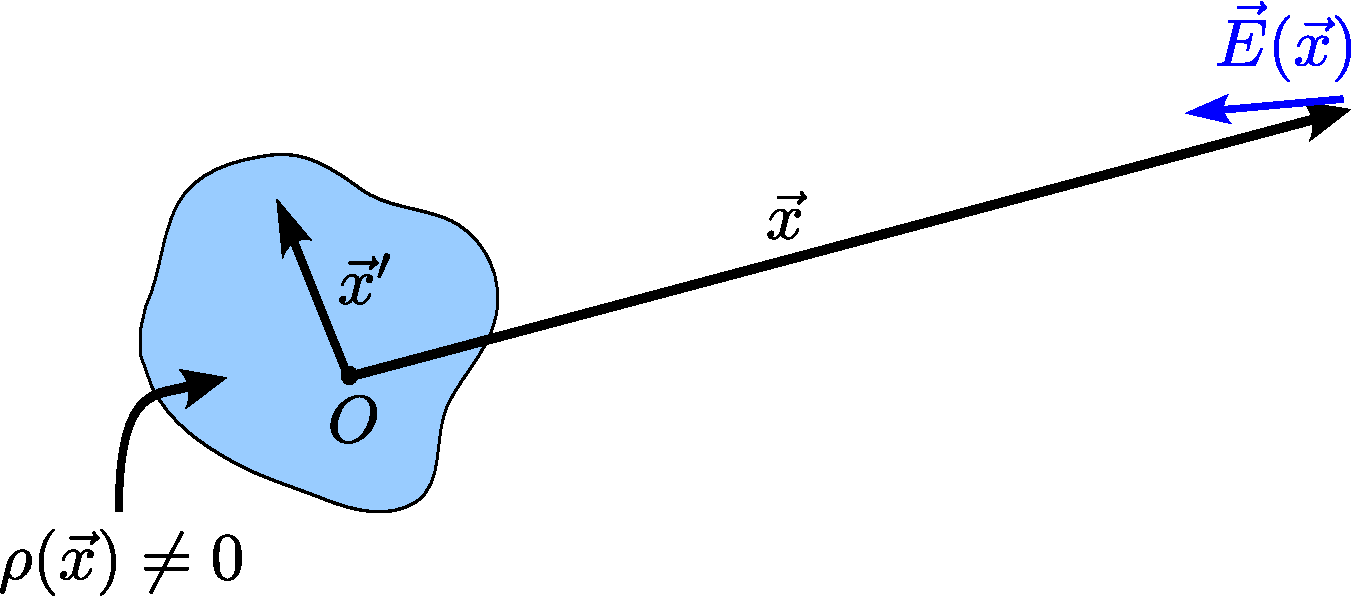
\psfig{file=fig/fig-expansion-multipolar-electrica-01.pdf,height=4cm,
angle=0 } }
\caption{Esquema de la expansi'on multipolar el'ectrica.}
\label{fig:emc}
\end{figure}
El m'etodo de {\em expansi'on multipolar} permite calcular los campos (potencial y campo el'ectrico) de una
\textit{distribuci'on compacta, pero arbitraria}, de carga en forma relativamente sencilla y general. Consideramos entonces una distribuci'on compacta de carga, situaremos (sin p'erdida de generalidad) el origen del sistema coordenado en un punto representativo de la distribuci'on (no necesariamente el centro de masa o el centro de carga), y consideraremos el problema de describir el
campo generado por esta distribuci'on en puntos muy alejados de ella, de modo
que $|\vec{x}|\gg|\vec{x}'|$, ver figura \ref{fig:emc}. Esto permite
reescribir la expresi'on general (\ref{perho}) para el potencial
el'ectrico, en forma de una expansi'on en serie, ya
que el t'ermino $1/\left|\vec{x}-\vec{x}'\right|$ puede ser expandido\footnote{Para esto usamos la expresi'on general para una expansi'on en serie de Taylor de una funci'on de varias variables: $f(x_i+x'_i)=f(x_i)+x'_i\left.(\partial_if)\right|_x+(1/2!)\,x'_ix'_j\left.(\partial_i\partial_jf)\right|_x +(1/3!)\,x'_ix'_jx'_k\left.(\partial_i\partial_j\partial_kf)\right|_x+\dots$.}
en potencias de las componentes del vector $\vec{x}'$:
\begin{eqnarray}
\frac{1}{\left|\vec{x}-\vec{x}'\right|}
%&=&\frac{1}{\left|\vec{x}\right|}
%+x'_i\partial'_i\left(\frac{1}{\left|\vec{x}-\vec{x}'\right|} \right)
%_{x'_i=0}+\frac{1}{2!}x'_ix'_j\,\partial'_i\partial'_j\left(\frac{1}{\left|\vec{
%x } -\vec{x}'\right|} \right) _{x'_i=0}+\dots \\
&=&\frac{1}{\left|\vec{x}\right|}
-x'_i\partial_i\left(\frac{1}{\left|\vec{x}-\vec{x}'\right|} \right)
_{x'_i=0}+\dots+(-1)^2\frac{1}{2!}x'_ix'_j\,
\partial_i\partial_j\left(\frac{1} { \left|\vec{x}-\vec{x}
'\right|} \right) _{x'_i=0}+\dots \\
&=&\frac{1}{\left|\vec{x}\right|}-x'_i\partial_i\frac{1}{\left|\vec{x}\right|}
 +\frac{(-1)^2}{2!}x'_ix'_j\,\partial_i\partial_j\frac{1}{\left|\vec{x}\right|}
+\dots \\
&=&\frac{1}{r}-x'_i\partial_i\frac{1}{r}+\frac{(-1)^2}{2!}x'_ix'_j\,
\partial_i\partial_j\frac{1}{r} +\dots \\
&=&\sum_{n=0}^\infty\frac{(-1)^n}{n!}x'_{i_1}\dots x'_{i_n}\partial_{i_1}\dots
\partial_{i_n}\frac{1}{r} .\label{exp1or}
\end{eqnarray}
Note que los t'erminos con derivadas de la forma $\partial_{i_1}\cdots
\partial_{i_n}r^{-1}$ son funciones (relativamente) simples y \textit{conocidas}.
Por ejemplo:
\begin{eqnarray}
\partial_i\frac{1}{r}&=&-\frac{x_i}{r^3}, \\
\partial_i\partial_j\frac{1}{r}
&=& \frac{3x_ix_j}{r^5}-\frac{\delta_{ij}}{r^3} \\
\partial_i\partial_j\partial_k\frac{1}{r}
&=& \frac{3\left(x_i\delta_{jk}+x_j\delta_{ki}+x_k\delta_{ij}\right)}{r^5}
-\frac{15x_ix_jx_k}{r^7},
\end{eqnarray}
etc. Con esto, podemos escribir
\begin{equation} \label{eq3.2.3}
\frac{1}{|\vec{x}-\vec{x}'|}=\frac{1}{r}+\frac{x_ix'_i}{r^3}
+\frac{1}{2}\,x'_ix'_j\,\left(\frac{3x_ix_j}{r^5}-\frac{\delta_{ij}}{
r^3}\right)+O\left(x_i'^3\right).
\end{equation}
En general, el t'ermino de orden $n$, $\partial_{i_1}\cdots
\partial_{i_n}r^{-1}$, decrecer'a con la distancia como $r^{-(n+1)}$.

Con la expansi'on (\ref{exp1or}) podemos reescribir la expresi'on
(\ref{perho}) para un potencial electrost'atico general (imponiendo $\phi=0$ en el infinito) como
\begin{eqnarray}
\phi(\vec x)&=&\frac{1}{4\pi\varepsilon_0}\int_V\frac{\rho(\vec x')}{
\left\vert \vec x-\vec x'\right\vert }dV'\\
&=&\frac{1}{4\pi\varepsilon_0}\int_V \rho(\vec
x')\sum_{n=0}^\infty\frac{(-1)^n}{n!}x'_{i_1}\dots x'_{i_n}\partial_{i_1}\cdots
\partial_{i_n}\frac{1}{r}dV'\\
&=&\frac{1}{4\pi\varepsilon_0}\sum_{n=0}^\infty\frac{(-1)^n}{n!}\left[\int_V
\rho(\vec x')\,x'_{i_1}\dots x'_{i_n}\,dV'\right]\partial_{i_1}\cdots
\partial_{i_n}\frac{1}{r}. \label{phimult}
\end{eqnarray}
Definiendo el momento multipolar de orden $n$ como el tensor de rango $n$ dado
por
\begin{equation}
\boxed{Q_{i_1\cdots i_n}:=\int_V \rho(\vec x)\,x_{i_1}\dots x_{i_n}\,dV,}
\end{equation}
podemos expresar un campo el'ectrost'atico general por medio de la
\textit{expansi'on multipolar}
\begin{equation}
 \boxed{\phi(\vec
x)=\frac{1}{4\pi\varepsilon_0}\sum_{n=0}^\infty\frac{(-1)^n}{n!}\,Q_{ i_1\cdots
i_n}\,\partial_{i_1}\cdots\partial_{i_n}\frac{1}{r}.} \label{phimult2}
\end{equation}
En otras palabras, podemos descomponer el potencial electrost'atico en una suma
de t'erminos de distinto orden en la expansi'on multipolar
\begin{equation}
 \boxed{\phi(\vec{x})=\sum_{n=0}^\infty\phi^{(n)}(\vec{x}),}
\end{equation}
donde $\phi^{(n)}(\vec{x})$ es la contribuci'on multipolar de orden $n$,
definida por
\begin{equation}
\boxed{\phi^{(n)}(\vec{x}):=\frac{1}{4\pi\varepsilon_0}\,\frac{(-1)^n}{n!}\,Q_{
i_1\cdots i_n}\,\partial_{i_1}\cdots\partial_{i_n}\frac{1}{r}.}
\end{equation}
Los primeros t'erminos de esta expansi'on general son de la forma:
\begin{equation} \label{eq3.2.4}
\phi(\vec{x})=\phi^0(\vec{x})+\phi^{(1)}(\vec{x})+\phi^{(2)}(\vec{x})+
\ldots.
\end{equation}
El t'ermino {\em monopolar} es
\begin{equation} \label{eq3.2.5}
\phi^0(\vec{x})=\frac{1}{4\,\pi\varepsilon_0}\,\frac{Q}{r},
\end{equation}
donde $Q$, el \textit{momento monopolar}, es simplemente la carga total del sistema:
\begin{equation} \label{eq3.2.6}
Q=\int \rho(\vec{x})\,dV.
\end{equation}
El segundo t'ermino, el t'ermino {\em dipolar} es dado por
\begin{equation}
\phi^{(1)}(\vec{x}) =\frac{1}{4\,\pi\varepsilon_0}\,\frac{x_i\,p_i}{r^3},
\end{equation}
donde $p_i:=Q_i$ es el \textit{momento dipolar} del sistema:
\begin{equation} \label{eq3.2.8}
p_i:=\int x_i\,\rho(\vec{x})\,dV.
\end{equation}
La tercera contribuci'on viene dada por el t'ermino {\em cuadrupolar}:
\begin{equation} \label{eq3.2.9}
\phi^{(2)}(\vec{x})=\frac{1}{4\,\pi\varepsilon_0}\,\frac{1}{2}\,Q_{ij}
\left(\frac{3\,x_i\,x_j}{r^5}-\frac{\delta_{ij}}{r^3}\right).
\end{equation}
El \textit{momento cuadrupolar} $Q_{ij}$ es dado por
\begin{equation}
Q_{ij}:=\int x_ix_j\,\rho(\vec{x})\,dV. \label{mom4}
\end{equation}
Con esto, la expansi'on multipolar del potencial es de la forma:
\begin{equation} \label{eq3.2.12}
\boxed{\phi(\vec{x})=\frac{1}{4\,\pi\varepsilon_0}\,\frac{Q}{r}+
\frac{1}{4\pi\varepsilon_0}\,\frac{\vec{p}\cdot\vec{x}}{r^3}+
\frac{1}{4\pi\varepsilon_0}\,\frac{1}{2}\,Q_{ij}\left(\frac{3\,x_i\,x_j}{
r^5}-\frac{\delta_{ij}}{r^3}\right)+O(r^{-4})}
\end{equation}
Podemos tambi'en encontrar una expansi'on multipolar para el campo el'ectrico
simplemente derivando el potencial. Con esto, obtenemos
\begin{align} \label{eq3.2.12.1}
E_i(\vec{x}) =& \frac{Q}{4\pi\varepsilon_0}\,\frac{x_i}{r^3}+\frac{1}{
4\pi\varepsilon_0}\,\frac{(3\,p_j\,x_j\,x_i-r^2\,p_i)}{r^5} \nonumber\\
& - \frac{1}{4\pi\varepsilon_0}\frac{1}{2}Q_{jk}\left[
\frac{3\left(x_i\delta_{jk}+x_j\delta_{ki}+x_k\delta_{ij}\right)}{r^5}
-\frac{15x_ix_jx_k}{r^7}\right]
+O(r^{-5}) .
\end{align}

Observaciones:

\begin{itemize} 
\item El momento multipolar de orden $n$, $Q_{i_1\dots i_n}$ es un tensor sim'etrico de rango $n$ respecto a transformaciones ortogonales de coordenadas. Por eso, $Q_{i_1\dots i_n}$ tiene $(n+1)(n+2)/2$ componentes linealmente independientes.

\item Los momentos multipolares son cantidades \textit{aditivas} (o extensivas). Esto quiere decir que si se divide un sistema en dos partes (el volumen donde est'an contenidas las cargas, en dos volumenes m'as peque\~nos o, equivalentemente, la densidad de carga en la suma de dos densidades) entonces cada momento multipolar (de un orden dado) es la suma de los momentos multipolares de cada subsistema.

\item Note que los momentos multipolares \textbf{dependen en general de la
elecci'on del origen}. Si se desplaza el origen del sistema coordenado de modo que el origen $O$ original tenga coordenadas $\vec{d}$ respecto al nuevo origen $O'$ entonces
$\vec{x}'=\vec{x}+\vec{d}$ y los nuevos momentos multipolares respecto al origen $O'$ est'an dados por:
\begin{eqnarray}
 Q'&=&Q,\\
Q'_i&=&Q_i+Qd_i,\\
Q'_{ij}&=&Q_{ij}+Q_id_j+Q_jd_i+Qd_id_j,
\end{eqnarray}
etc.
\end{itemize}

\subsubsection{Momento cuadrupolar sin traza}\label{MCSM}
El momento cuadrupolar (\ref{mom4}) es un tensor \textit{sim'etrico}, por lo
que tiene ${3\cdot (3+1)}/{2}=6$ componentes linealmente independientes (que
hay que calcular!). Sin embargo, debido a que este tensor siempre est'a
multiplicado en la expansi'on multipolar del potencial por
$\left({3\,x_i\,x_j}/{r^5}-{\delta_{ij}}/{r^3}\right)$, puede
verificarse que no todas las componentes de $Q_{ij}$ contribuyen a la
expansi'on multipolar. En efecto, debido a que la contracci'on
$\delta_{ij}\left({3\,x_i\,x_j}/{r^5}-{\delta_{ij}}/{r^3}\right)$ se
anula \textit{id'enticamente}, es posible sumar un t'ermino proporcional a
$\delta_{ij}$ al momento cuadrupolar, sin por ello alterar la expansi'on
multipolar. En otras palabras, existe una libertad para redefinir el momento
cuadrupolar ya que $\tilde{Q}_{ij}:=Q_{ij}+\lambda\delta_{ij}$ puede ser
considerado como un momento cuadrupolar 'util y leg'itimo. 

Una posibilidad ser'ia elegir $\lambda\stackrel{!}{=}-Q_{ii}$, en cuyo caso obtendr'iamos
\begin{equation}
 \boxed{Q'_{ij}=\int
(x_ix_j-x_kx_k\delta_{ij})\,\rho(\vec{x})\,dV,}
\end{equation}
que, salvo un signo global, tiene la misma forma que el conocido tensor momento de inercia asociado a un cuerpo en rotaci'on. En este sentido, el momento cuadrupolar el'ectrico es el an'alogo al tensor momento de inercia en mec'anica.

Sin embargo, es m'as com'un explotar la libertad para elegir $\lambda$ para definir el  \textit{momento cuadrupolar libre de traza}, definido tal que $\tilde{Q}_{ii}\equiv 0$. Esto equivale a considerar $\lambda\stackrel{!}{=}-Q_{ii}/3$, es decir, $\tilde{Q}_{ij}=Q_{ij}-Q_{kk}\,\delta_{ij}/3$ o,
m'as expl'icitamente:
\begin{equation}
 \boxed{\tilde{Q}_{ij}=\int
(x_ix_j-\frac{1}{3}x_kx_k\delta_{ij})\,\rho(\vec{x})\,dV.} \label{mom4st}
\end{equation}
La ventaja de usar este tensor es que, por ser libre de traza, s'olo tiene 5
componentes linealmente independientes (que calcular, por ejemplo:
$\tilde{Q}_{11}$, $\tilde{Q}_{12}$, $\tilde{Q}_{13}$, $\tilde{Q}_{22}$,
$\tilde{Q}_{23}$, ya que $\tilde{Q}_{21}=\tilde{Q}_{12}$,
$\tilde{Q}_{31}=\tilde{Q}_{13}$, $\tilde{Q}_{32}=\tilde{Q}_{23}$ y
$\tilde{Q}_{33}=-\tilde{Q}_{11}-\tilde{Q}_{22}$) (pero, por otro lado, la integral que se necesita calcular es algo m'as complicada).

Adem'as, el momento cuadrupolar (con o sin traza), por ser un tensor \textit{sim'etrico} de segundo rango, puede ser diagonalizado, es decir, es posible encontrar sus vectores (y valores) propios, que definen direcciones ``principales'', ortogonales entre si. En el sistema coordenado definido por estas tres direcciones principales el momento cuadrupolar adopta una forma diagonal.


\subsubsection{Monopolo ideal}
Una carga puntual es un ``monopolo ideal"\,, ya que (eligiendo el origen en la posici'on de la carga) el 'unico momento distinto de cero es el momento monopolar. 

\subsubsection{Dipolo ideal}
Un ``dipolo ideal"\,(tambi'en llamado ``dipolo puntual'') es un sistema idealizado cuyo 'unico momento multipolar el'ectrico no nulo es el momento dipolar.

El sistema formado por una carga $q^{(1)}=-q$ y otra $q^{(2)}=+q$, separados una distancia $d$ tiene momento monopolar nulo, mientras que 
\begin{equation}
p_i=(-q)x^{(1)}_i+(+q)x^{(2)}_i=q(x^{(2)}_i-x^{(1)}_i)=qd_i,
\end{equation}
\begin{equation}
Q_{ij}=(-q)x^{(1)}_i x^{(1)}_j +(q)x^{(2)}_i x^{(2)}_j,
\end{equation}
\begin{equation}
Q_{ijk}=(-q)x^{(1)}_i x^{(1)}_jx^{(1)}_k +(q)x^{(2)}_i x^{(2)}_jx^{(2)}_k,
\end{equation}
etc. En el l'imite $\vec{d}\to\vec{0}$, pero tal que $\vec{p}$ sea finito (esto, por supuesto, requiere $q\to\infty$), tendremos que $Q_{ij}\to 0$, $Q_{ijk}\to 0$, y lo mismo ocurrir'a para todo momento multipolar de orden superior  (las componentes del momento multipolar de orden $n$ son en este caso proporcionales a $qd^n=pd^{n-1}$).

\begin{equation}\label{phip}
\phi_{\vec{p}}(\vec{x})=\frac{1}{4\pi\varepsilon_0}\frac{(x_j-x_j')p_j}
{|\vec{x}-\vec{x}'|^3},
\end{equation}
\begin{figure}[H]
\begin{center}
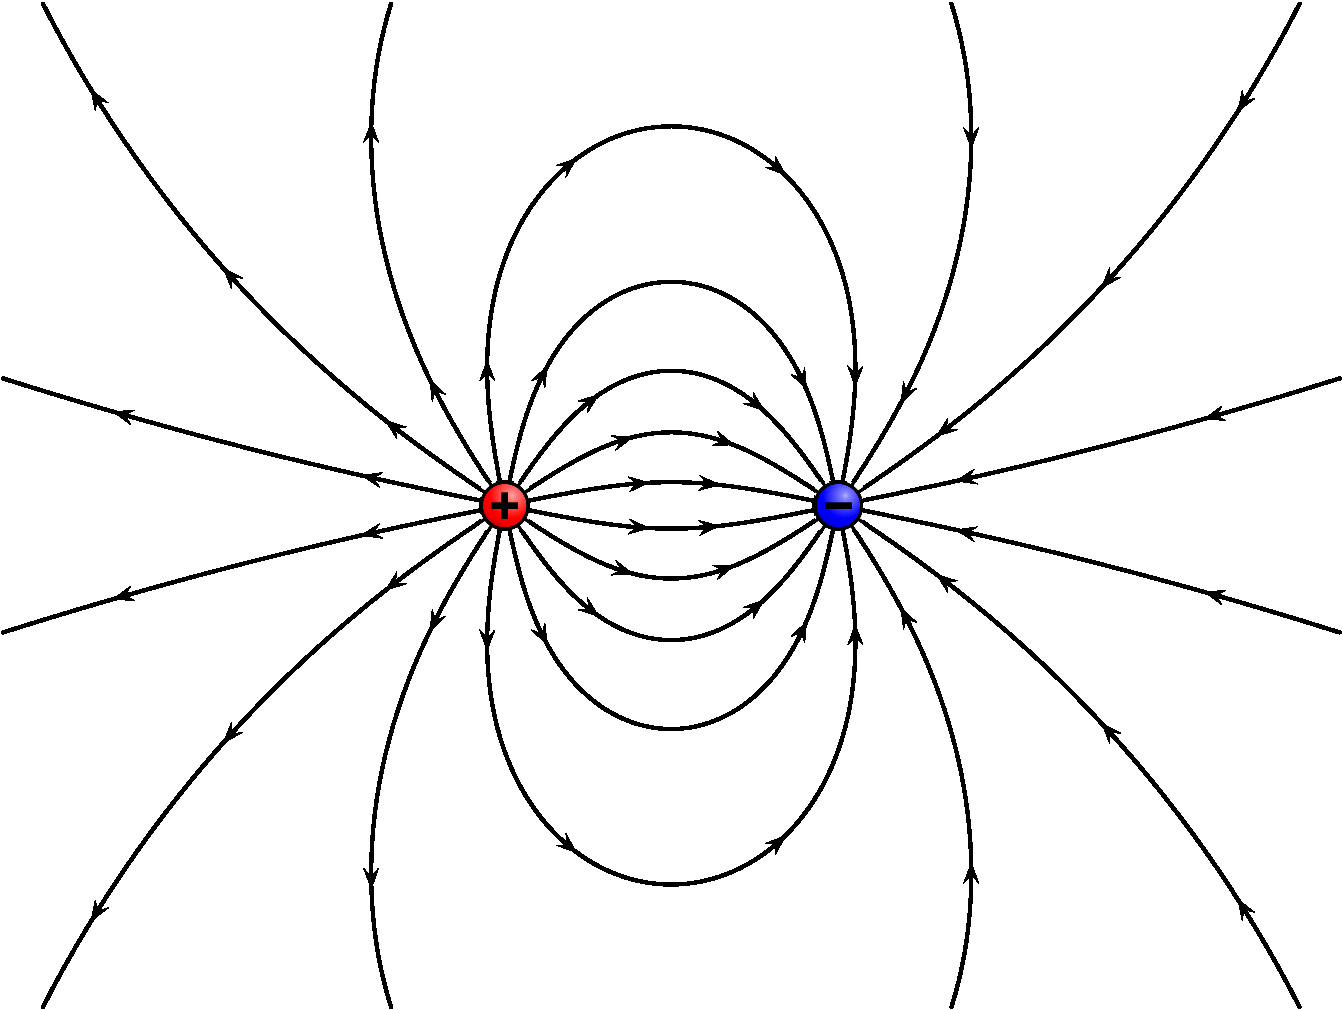
\includegraphics[height=4cm]{fig/fig-E-02.pdf}\hspace{1cm}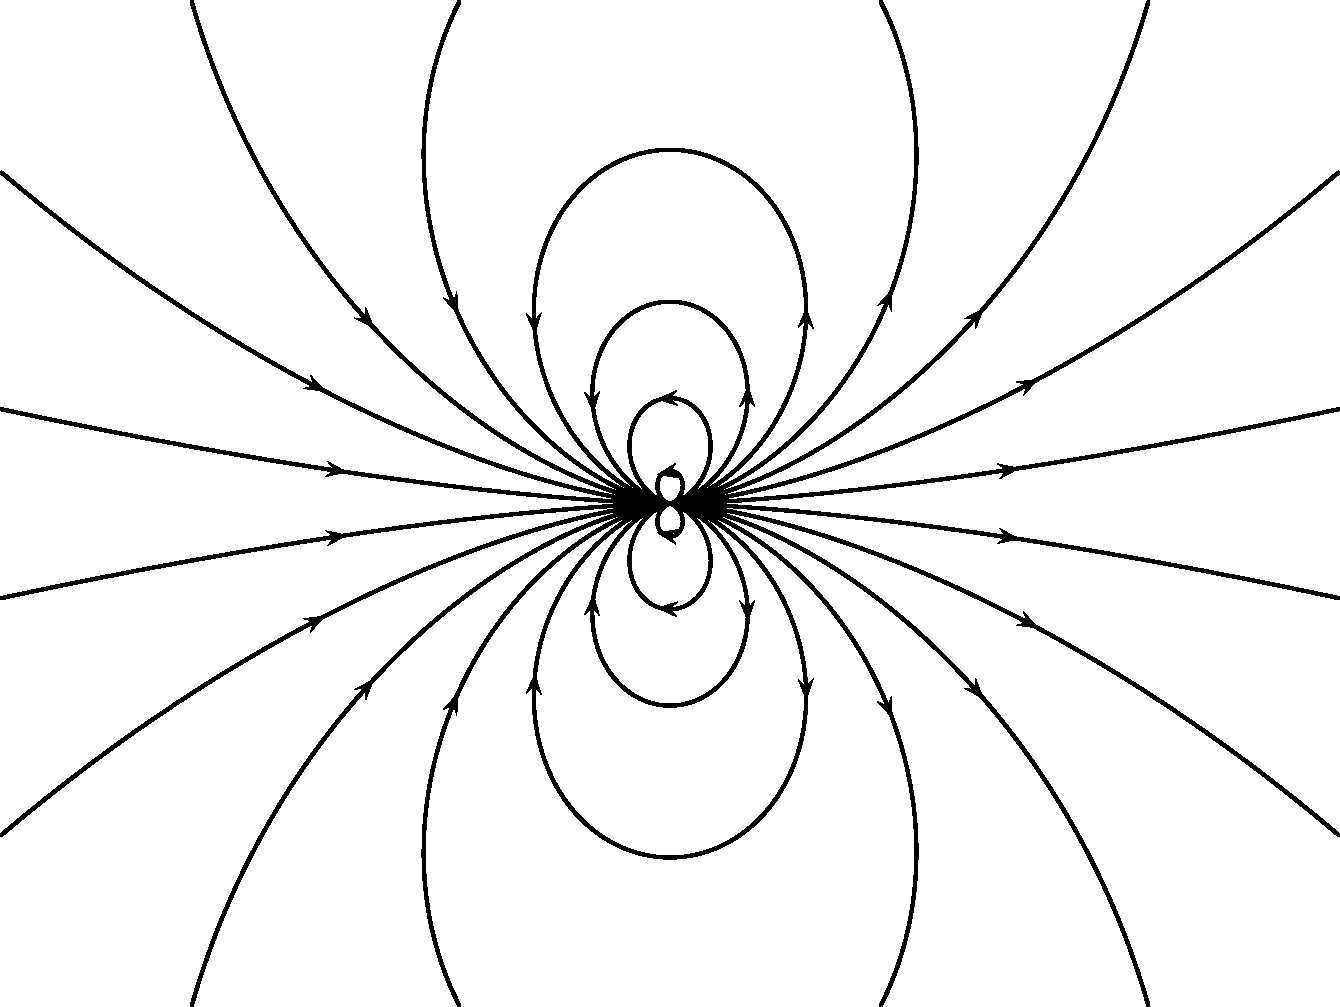
\includegraphics[height=4cm]{fig/fig-campo-dipolo-electrico.pdf} 
\caption{Dipolo (dos cargas opuestas) versus dipolo ideal. Figuras creadas usando VectorFieldPlot \cite{VFP}.}
\label{fig-dipolos}
\end{center}
\end{figure}
\subsubsection{Cuadrupolo ideal}
$Q=0$ $p_i=0$, $Q_{ij}\neq 0$, $Q_{ijk}=0$, etc.

\begin{figure}[H]
\begin{center}
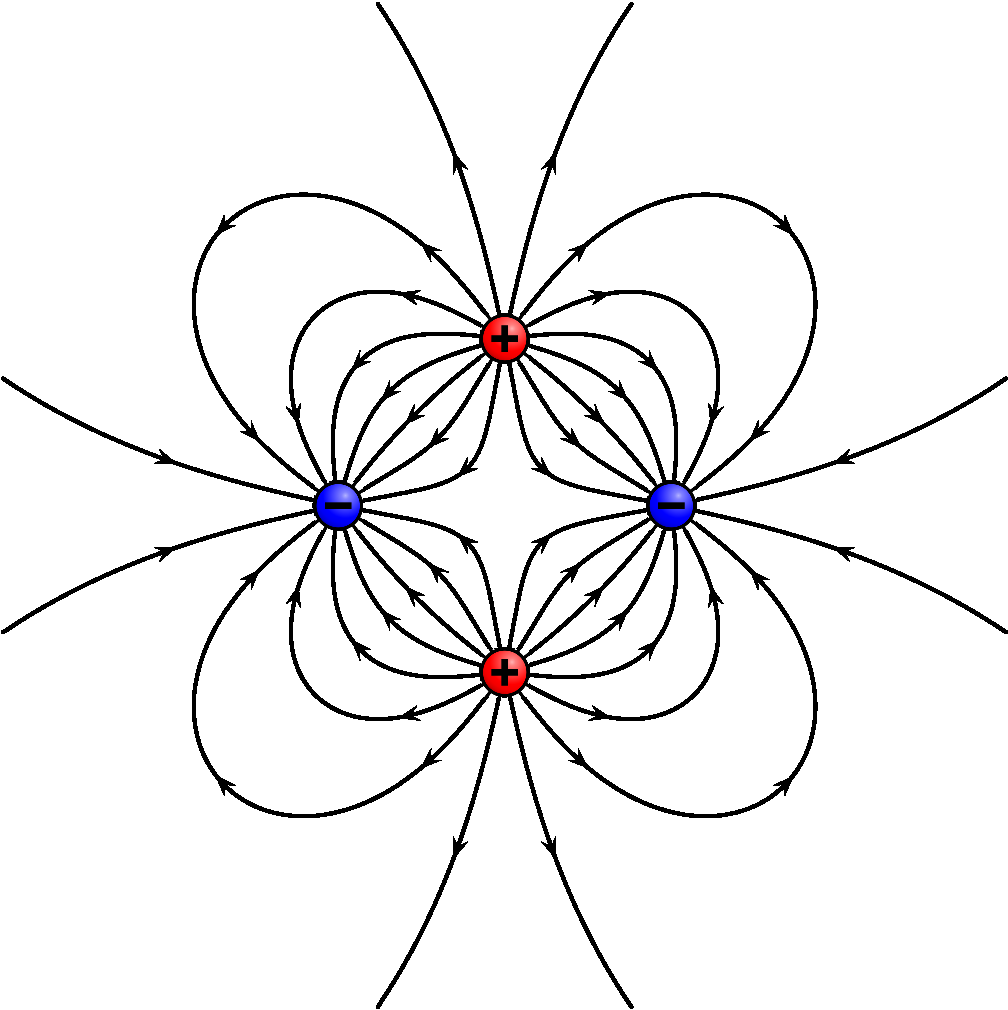
\includegraphics[height=4cm]{fig/fig-E-03.pdf}\hspace{1cm}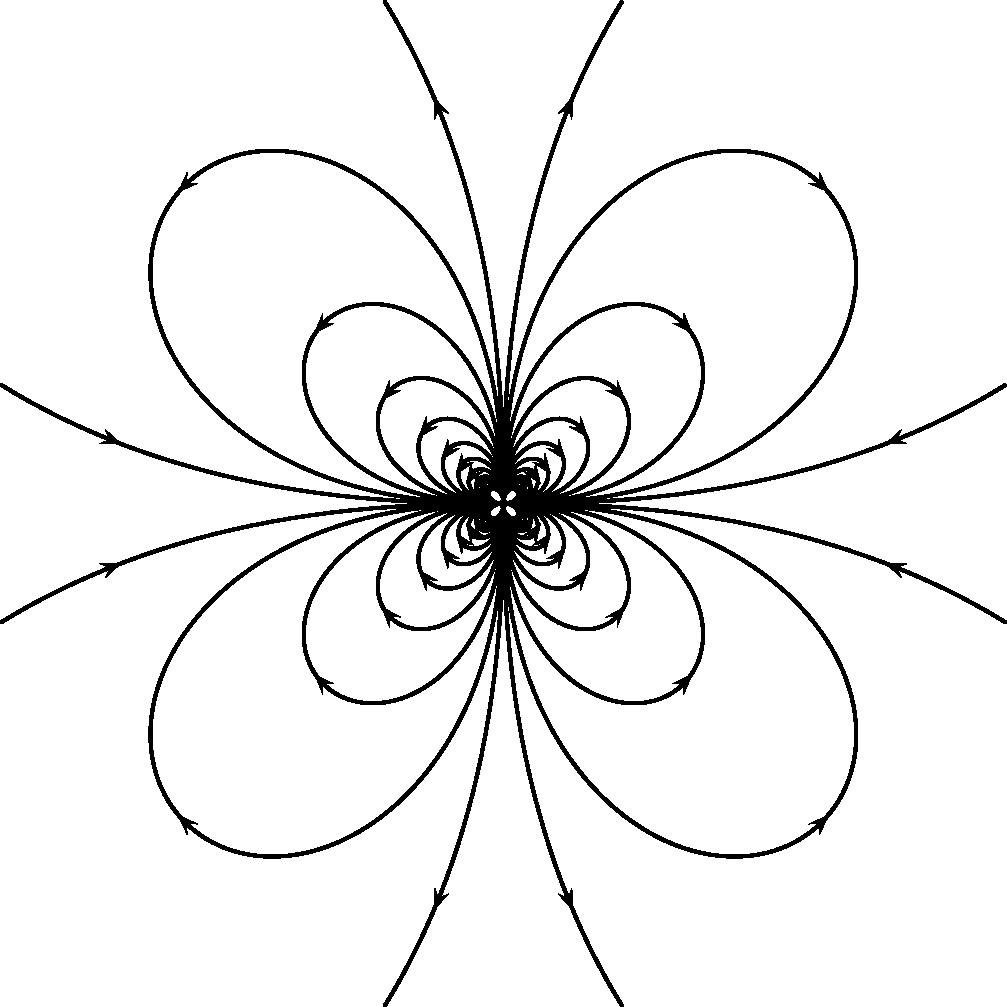
\includegraphics[height=4cm]{fig/fig-campo-cuadrupolo-electrico-ideal.pdf} 
\caption{Cuadrupolo versus cuadrupolo ideal. Figuras creadas usando VectorFieldPlot \cite{VFP}.}
\label{fig-dipolos}
\end{center}
\end{figure}
\newpage


\subsection{Distribuciones de carga en campos externos} \label{ed3_3}

En las secciones anteriores hemos considerado la expansi'on multipolar
\textit{generada} por una distribuci'on compacta de carga
$\rho(\vec{x})$. Ahora discutiremos una situaci'on distinta: consideraremos
una (peque\~na) distribuci'on de cargas en un campo el'ectrico
\textit{externo} (es decir, generado por alguna \textit{otra} distribuci'on de
carga). En particular, calcularemos la energ'ia potencial de la
distribuci'on de carga en el campo externo dado, as'i como la fuerza y el
torque que el campo externo ejerce.

\subsubsection{Energ'ia Potencial} \label{ed3_3_1}


Para evaluar esta integral, consideramos un \textit{punto representativo $P$ de la
distribuci'on} con coordenadas $\vec{x}$ y un punto $P'$ cualquiera de la
distribuci'on  (con coordenadas $\vec{x}+\vec{x}'$ respecto
al origen, ver figura) determinado por el vector $\vec{x}'$ respecto al punto
representativo $P$ de la distribuci'on, y expandiremos los valores $\phi(P')$ en
una serie de Taylor en torno a $P$:
\begin{align} \label{eq3.3.3}
\phi(P') = &\ \phi(\vec{x}+\vec{x}')\\
= & \sum_{n=0}^\infty\frac{1}{n!}x'_{i_1}\cdots
x'_{i_n}\left.(\partial_{i_1}\cdots\partial_{i_n}\phi)\right|_{\vec{x}'=\vec{0}} \\
= &\ \left.\phi\right|_{\vec{x}'=\vec{0}}+x'_i\left.(\partial_i\phi)\right|_{\vec{
x}'=\vec{0}}+\frac{1}{2}x'_ix'_j\left.(\partial_i\partial_j\phi)\right|_{\vec{x}
'=\vec{0}}+\cdots \nonumber\\
& +\frac{1}{n!}x'_{i_1}\cdots
x'_{i_n}\left.(\partial_{i_1}\cdots\partial_{i_n}\phi)\right|_{\vec{x}'=\vec{0}}
+\cdots\\
= &\ \phi(\vec{x})-x'_iE_i(\vec{x})-\frac{1}{2}x'_ix'_j(\partial_iE_j)(\vec{x}
) \nonumber \\
& -\cdots-\frac{1}{n!}x'_{i_1}\cdots
x'_{i_n}(\partial_{i_1}\cdots\partial_{i_{n-1}}E_{i_n})(\vec{x})+\cdots .
\end{align}

Con esto, podemos escribir (\ref{Urhophiext}) como
\begin{eqnarray}
 U&=&\int\rho(P')\,\phi(P')\,dV'\\
&=&\sum_{n=0}^\infty\frac{1}{n!}\left[\int\rho(P')x'_{i_1}\cdots
x'_{i_n}\,dV'\right]\left.(\partial_{i_1}\cdots\partial_{i_n}\phi)\right|_{\vec{x}'=\vec{0}}\\
%&=&\left[\int\rho(\vec{x}')
%\phi(\vec{x})-\left[\int\rho(\vec{x}')\,
%x'_i\,dV'\right] E_i(\vec{x})-\frac{1}{2}\left[ \int\rho(\vec{x}')\,
%x'_ix'_j\,dV'\right](\partial_iE_j)(\vec{x})
%\nonumber\\
%&&-\cdots-\frac{1}{n!}\left[ \int\rho(\vec{x }')\, x'_{i_1}\cdots
%x'_{i_n}\,dV'\right] (\partial_{i_1}
%\cdots\partial_{i_{n-1}}E_{i_n})(\vec{x})+\cdots \\
&=&\sum_{n=0}^\infty\frac{1}{n!}Q_{i_1\cdots i_n}(\partial_{i_1}\cdots\partial_{i_n}\phi)(\vec{x})\\
&=&Q\phi(\vec{x})-Q_iE_i(\vec{x})-\frac{1}{2}
Q_{ij}(\partial_iE_j)(\vec{x}) \nonumber \\
&& -\cdots-\frac{1}{n!}Q_{i_1\cdots i_n}(\partial_{i_1}
\cdots\partial_{i_{n-1}}E_{i_n})(\vec{x})+\cdots .
\end{eqnarray}
Por lo tanto, obtenemos que la energ'ia potencial de una distribuci'on de
carga, caracterizada por sus momentos multipolares, en un \textit{campo externo}
es dado por
\begin{equation} \label{eq3.3.4}
\boxed{U=Q\,\phi(\vec{x})-\vec{p}\cdot\vec{E}(\vec{x})-\frac{1}{2}\,Q_{ij}
\,\partial_iE_j(\vec{x})+\cdots .}
\end{equation}

El primer t'ermino de esta expansi'on, la contribuci'on monopolar, es
equivalente a la de una carga \textit{puntual} en un potencial externo. El
t'ermino siguiente (dipolar) representa la energ'ia potencial de un dipolo
ideal en un campo el'ectrico externo. Note que este t'ermino es m'inimo cuando
el momento dipolar es paralelo al campo el'ectrico externo (y es, en general,
proporcional al coseno del 'angulo entre $\vec{p}$ y $\vec{E}$). El t'ermino
cuadrupolar es distinto de cero s'olo cuando el campo es inhomog'eneo. Note que
en esta expresi'on tambi'en es posible usar un momento cuadrupolar redefinido
como se discuti'o en la secci'on (\ref{MCSM}). En particular puede usarse el
momento cuadrupolar sin traza. La energ'ia potencial calculada usando distintos
momentos cuadrupolares equivalentes es la misma puesto que un t'ermino
proporcional a $\delta_{ij}$ contribuira con un t'ermino proporcional a
$\delta_{ij}(\partial_iE_j)=\partial_iE_i$, que es cero en virtud de la ley de
Gauss y el hecho que $\vec{E}$ describe un \textit{campo el'ectrico externo},
es decir, un campo generados por fuentes fuera de la regi'on bajo
consideraci'on.


\subsubsection{Fuerza}  \label{ed3_3_2}

Una carga puntual $q$ experimenta una fuerza
$\vec{F}(\vec{x})=q\,\vec{E}(\vec{x})$ cuando est'a situada en
un punto donde existe un campo externo $\vec{E}(\vec{x})$. Como consecuencia,
la fuerza total sobre una distribuci'on con densidad $\rho$ en un campo
\textit{externo} puede escribirse como
\begin{equation} \label{eq3.3.7}
F_i=\int \rho(P')\,E_i(P')\,dV'.
\end{equation}
Expandimos $E_i(P')$ en serie de Taylor, de forma similar a como lo
hicimos en la secci'on anterior con el potencial
\begin{equation} \label{eq3.3.7.1}
E_i(P')=E_i(\vec{x})+x'_j(\partial_jE_i)(\vec{x})+\frac{1}{
2}x'_jx'_k(\partial_j\partial_kE_i)(\vec{x})
+\cdots+\frac{1}{n!}x'_{i_1}\cdots
x'_{i_n}(\partial_{i_1}\cdots\partial_{i_n}E_i)(\vec {x})+\cdots .
\end{equation}
Con esto, podemos reescribir (\ref{eq3.3.7}) como
\begin{eqnarray}
F_i&=& \int
\rho(P')\,\left[E_i(\vec{x})+x'_j(\partial_jE_i)(\vec{x})+\frac{1}{
2}x'_jx'_k(\partial_j\partial_kE_i)(\vec{x}) \right.\nonumber\\
&& \quad\qquad\qquad \left. +\cdots+\frac{1}{n!}x'_{i_1}\cdots
x'_{i_n}(\partial_{i_1}\cdots\partial_{i_n}E_i)(\vec {x})+\cdots\right] dV' \\
&=&
Q\,E_i(\vec{x})+p_j(\partial_jE_i)(\vec{x})+\cdots+\frac{1}{n!}Q_{i_1\cdots i_n}
(\partial_{i_1}\cdots\partial_{i_n}E_i)(\vec {x})+\cdots .\label{eq3.3.8}
\end{eqnarray}
El primer t'ermino, $Q\vec{E}(\vec{x})$, es nuevamente la contribuci'on monopolar correspondiente a la fuerza sobre una carga puntual. La contribuci'on
dipolar es ahora proporcional al gradiente del campo el'ectrico. Usando el hecho que el campo electrost'atico satisface
$\partial_iE_j=\partial_jE_i$ podemos expresar el t'ermino dipolar como $\partial_i(p_jE_j)$,
es decir.
\begin{equation} \label{eq3.3.12}
\boxed{\vec{F}(\vec{x}) =
Q\vec{E}(\vec{x})-\vec{\nabla}\left(-\vec{p}\cdot\vec{E}(\vec{x})\right)+\cdots.
}
\end{equation}
Note que el segundo t'ermino es el gradiente de la contribuci'on dipolar a la
energ'ia potencial de la distribuci'on.

\subsubsection{Torque}  \label{ed3_3_3}

An'alogamente al caso de la fuerza total, podemos calcular el \textit{torque
neto} ejercido por el campo externo sobre la distribuci'on, respecto del punto
representativo que hemos considerado:
\begin{equation}
\vec{\tau} = \int \rho(P')\,\vec{x}'\times\vec{E}(P')\,dV' .
\end{equation}
En componentes, y usando la expansi'on (\ref{eq3.3.7.1}) obtenemos
\begin{eqnarray}
\tau_i &=& \varepsilon_{ijk}\int\rho(P')x'_jE_k(P')\,dV' \\
&=&\varepsilon_{ijk}\int\rho(P')x'_j\left[
E_k(\vec{x})+x'_l(\partial_lE_k)(\vec{x})+\frac{1}{2}
x'_lx'_m(\partial_l\partial_mE_k)(\vec{x}) \right.\nonumber\\
&&\quad\qquad\qquad\qquad\left.+\cdots+\frac{1}{n!}x'_{i_1}\cdots
x'_{i_n}(\partial_{i_1}\cdots\partial_{i_n}E_k)(\vec
{x})+\cdots\right] \,dV' \\
&=&\varepsilon_{ijk}\left[p_j
E_k(\vec{x})+Q_{jl}(\partial_lE_k)(\vec{x})+\frac{1}{2}
Q_{jlm}(\partial_l\partial_mE_k)(\vec{x})\right.\nonumber\\
&&\quad\qquad\qquad\qquad\left.+\cdots+\frac{1}{n!}Q_{ji_1\cdots i_n}(\partial_{i_1}\cdots\partial_{i_n}
E_k)(\vec
{x})+\cdots\right] .
\end{eqnarray}
Por lo tanto,
\begin{equation}
\label{eq3.3.14}
\boxed{\vec{\tau}=\vec{p}\times\vec{E}(\vec{x})+\cdots. }
\end{equation}
Es posible expresar la primera contribuci'on (dipolar) al torque como un
``gradiente'' del t'ermino dipolar de la energ'ia potencial
$U_{\vec{p}}=-\vec{p}\cdot\vec{E}$, esta vez, sin embargo, no respecto a
variaciones de la posici'on $\vec{x}$ de la distribuci'on, sino con respecto a
cambios en la orientaci'on del momento dipolar respecto al campo
externo. La magnitud del torque es dada por
\begin{eqnarray}
\tau &=& pE\sen\theta \nonumber \\
&=& -\frac{d}{d\theta}\,\left(pE\cos\theta\right)\\
&=&\frac{dU_{\vec{p}}}{d\theta}.  \label{eq3.3.15}
\end{eqnarray}

\newpage


\newpage

\section{Electrost'atica macrosc'opica}
Hasta ahora hemos estudiado las propiedades de los campos
electrost'aticos \textit{en el vac'io} y en el interior de \textit{condutores ideales}.
Estamos ahora interesados en las propiedades el campo el'ectrico \textit{macrosc'opico} en el interior de un material \textit{aislante}. El t'ermino macrosc'opico se refiere al campo promedio en una peque\~na regi'on que, sin embargo, es grande comparada con el tama\~no de las mol'eculas que constituyen el material.

Consideraremos entonces materiales aislantes, tambi'en llamados \textit{diel'ectricos}, en los que las cargas internas no tienen la
libertad de desplazarse distancias macrosc'opicas (conducir) en presencia de un
campo el'ectrico aplicado, sino que est'an confinadas por la estructura
at'omica/molecular del material. La mayor'ia de los materiales son, en buena
aproximaci'on, diel'ectricos.

En presencia de un campo el'ectrico los diel'ectricos \textit{redistribuyen sus cargas} constituyentes. 'Estas no pueden desplazarse distancias macrosc'opicas,
como ocurre en los conductores, sino s'olo distancias del orden de magnitud determinado por su estructura molecular.
Estos peque\~nos desplazamientos de carga tienen, sin embargo, consecuencias
que se acumulan hasta ser perceptibles a escalas macrosc'opicas.
Concretamente, en presencia de un campo el'ectrico, el material
se \textit{polariza}.
El campo el'ectrico que causa (el cambio en) la polarizaci'on puede ser un campo ``externo'' (producido por ``cargas externas''\footnote{Tambi'en llamadas ``cargas libres'' o ``cargas no ligadas''.}, que no forman parte
de la estructura at'omica/molecular caracter'istica del medio).
\begin{figure}[!h]
\centerline{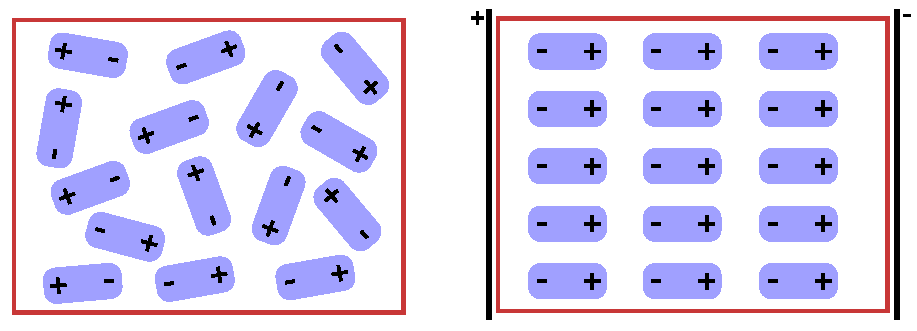
\psfig{file=fig/fig-dielectrico-01.pdf,height=4cm,angle=0}}
\caption{Un material diel'ectrico se polariza en presencia de un campo externo.}
\label{diel01}
\end{figure}

El campo el'ectrico total (``EL''\, campo el'ectrico) es influenciado por
la polarizaci'on del medio. Modelaremos este campo el'ectrico
(macrosc'opico) $\vec{E}$ como la suma del campo
producido por las cargas externas y el campo producido por la distribuci'on
de \textit{cargas de polarizaci'on} (descrita por el vector de polarizaci'on $\vec{P}$) del medio.

\subsection{Vector y cargas de Polarizaci'on}

Se define el \textit{vector de polarizaci'on} como la \textit{densidad de
momento dipolar} (momento dipolar por unidad de volumen),
\begin{equation}\label{defP}
\vec{P}(x):= ``\lim_{\Delta V\to 0}" \frac{\Delta\vec{p}}{\Delta V},
\end{equation}
donde $\Delta\vec{p}$ es el \textit{momento dipolar total de las cargas del material contenidas en el volumen} $\Delta V$. La regi'on con volumen $\Delta V$ se considera centrada en el punto $\vec{x}$, suficientemente peque\~na desde el punto de vista macrosc'opico, pero grande comparada con la escala  determinada por la estructura at'omica/molecular del material. Equivalentemente, el vector de polarizaci'on es definido tal que el momento dipolar $d\vec{p}$ en un elemento de volumen (macrosc'opico) $dV$ es dado por $d\vec{p}=\vec{P}(\vec{x})dV$.

Como consecuencia de la definici'on anterior, el momento dipolar
total de las cargas contenidas en un volumen finito $V$ es dado por
\begin{equation}\label{pintPdV}
 \vec{p}_V=\int_V \vec{P}(x)\,dV.
\end{equation}
Por otro lado, sabemos que el potencial generado por un dipolo ideal de momento dipolar $\vec{p}$ ubicado en un punto con coordenadas $\vec{x}'$ es de la forma \eqref{phip}. Luego, el potencial generado por una peque\~na regi'on de un medio polarizado con elemento de volumen $dV'$ y polarizaci'on $\vec{P}$ es dada por
\begin{equation}
d\phi(x)=\frac{1}{4\pi\varepsilon_0}\frac{(x_j-x_j')P_j(x')\,dV'}{|\vec{x}-\vec{
x}'|^3}.
\end{equation}
De esta forma, si el sistema contiene adem'as cargas libres en $dV'$ entonces
\begin{equation}
d\phi(x)=\frac{1}{4\pi\varepsilon_0}\frac{\rho_{\rm
ext}(x')}{|\vec{x}-\vec{x}'|}dV'+\frac {1}{
4\pi\varepsilon_0}\frac{P_i(x')(x_i-x_i')}{|\vec{x}-\vec{x}'|^3}dV'.
\end{equation}
Por lo tanto, el potencial (macrosc'opico, total), de acuerdo a nuestro modelo, es dado por
\begin{equation}
\boxed{\phi(x)=\frac{1}{4\pi\varepsilon_0}\int\left[\frac{\rho_{\rm
ext}(x')}{|\vec{x}-\vec{x}'|}+\frac{P_i(x')(x_i-x_i')}{|\vec{x}-\vec{x}'|^3}\right]dV'.}
\end{equation}
Usando la identidad (\ref{id01}) podemos escribir
\begin{align}
\frac{P_i(x')(x_i-x_i')}{|\vec{x}-\vec{x}'|^3}  &
=P_i(x')\partial_i'\left(  \frac{1}{|\vec{x}-\vec{x}'|}\right)\\
&=\partial_i'\left(\frac{P_i(x')}{|\vec{x}-\vec{x}'|}\right)-\frac{
(\partial_i'P'_i)(x')} {|\vec{x}-\vec{ x}'|}.
\end{align}
De esta forma, considerando que la integral sobre los t'erminos que dependen de la polarizaci'on est'an confinados al volumen $V$ del material (lo que no necesariamente es as'i para el t'ermino conteniendo las cargas libres), podemos escribir
\begin{align}
\phi(x)& =\frac{1}{4\pi\varepsilon_0}\int\frac{\rho_{\rm ext}(x')}{|x_i-x_i'|}dV'-\frac{1}{4\pi\varepsilon_0}\int_V\frac{1}
{|\vec{x}-\vec{x}'|}\partial_i'P_idV'+\frac{1}{4\pi\varepsilon_0}\int_{
\partial V}\frac{P_i(x')}{|\vec{x}-\vec{x}'|}\,dS'_i \\
& =\frac{1}{4\pi\varepsilon_0}\int\frac{\rho_{\rm ext}(x')}{|x_i-x_i'|}dV'+\frac{1}{4\pi\varepsilon_0}\int_V\frac{\rho_P(x')}{|x_i-x_i'|}dV'+\frac{1}{4\pi\varepsilon_0}\int_{
\partial V}\frac{\sigma_P(x')}{|\vec{x}-\vec{x}'|}\,dS' .
\end{align}
La expresi'on anterior muestra que el campo (macrosc'opico) total es
\textit{equivalente} al campo producido por una densidad volum'etrica de carga total,
\begin{equation}
\rho_{\rm T}:=\rho_{\rm ext}+\rho_P, \label{rhotot}
\end{equation}
donde
\begin{equation}
\boxed{\rho_P:=-\vec{\nabla}\cdot\vec{P},}
\end{equation}
es la \textit{densidad (volum'etrica) de carga de polarizaci'on}, (definida en cada punto del material), m'as una
\textit{densidad de carga de polarizaci'on de superficie},
\begin{equation}
\boxed{\sigma_P:=\vec{P}\cdot\hat{n},}
\end{equation}
distribuida en la superficie $S=\partial V$ del diel'ectrico.

Note que la carga total de polarizaci'on, tal como se espera, es nula:
\begin{equation}
 Q_P=\int_V\rho_P\,dV+\oint_{\partial V} \sigma_P\,dS\equiv 0,
\end{equation}
en virtud del teorema de Gauss.

\subsection{Desplazamiento el'ectrico}
Usando (\ref{rhotot}) en la ley de Gauss, podemos escribir
\begin{align*}
\vec\nabla\cdot\vec{E} &=\frac{1}{\varepsilon_0}\rho_T \\
&=\frac{1}{\varepsilon_0}\left( \rho_{\rm ext}-\vec\nabla\cdot\vec{P}\right).
\end{align*}
Luego,
\begin{equation}
 \vec\nabla\cdot\left(\vec{E}+\frac{1}{\varepsilon_0}\vec{P}\right)=\frac{\rho_{
\rm ext}(x)}{\varepsilon_0}.
\end{equation}
Definimos el \textit{vector de desplazamiento el'ectrico} (tambi'en llamado
\textit{excitaci'on el'ectrica} o \textit{inducci'on el'ectrica}) como
\begin{equation}\marginnote{Vector Desplazamiento}
 \boxed{\vec{D}(\vec{x}):=\varepsilon_0\vec{E}(\vec{x})+\vec{P}(\vec{x}),} \label{defD}
\end{equation}
de modo que
\begin{equation}
\boxed{\vec{\nabla}\cdot\vec{D}=\rho_{\rm ext}.} \label{divD}
\end{equation}
Las unidades del vector desplazamiento son de carga por unidad de 'area: 
$[\vec{D}]=[\vec{P}]=[\sigma]\stackrel{\text{
S.I.}}{=}{C}/{m^2}$.

La utilidad de usar $\vec{D}$ en lugar de $\vec{E}$ en esta ``ley de Gauss"
\,\eqref{divD} es que esta relaci'on \textit{s'olo involucra expl'icitamente a las cargas externas} (que son usualmente conocidas y/o controlables). Por ejemplo, como consecuencia de (\ref{divD}) tenemos que
\begin{equation}
 \boxed{\oint_S \vec{D}\cdot d\vec{S}=q_{\rm ext}.} \label{GaussD}
\end{equation}

\subsubsection{Ejemplo: Esfera diel'ectrica is'otropa y carga central}
\begin{figure}[!h]
\centerline{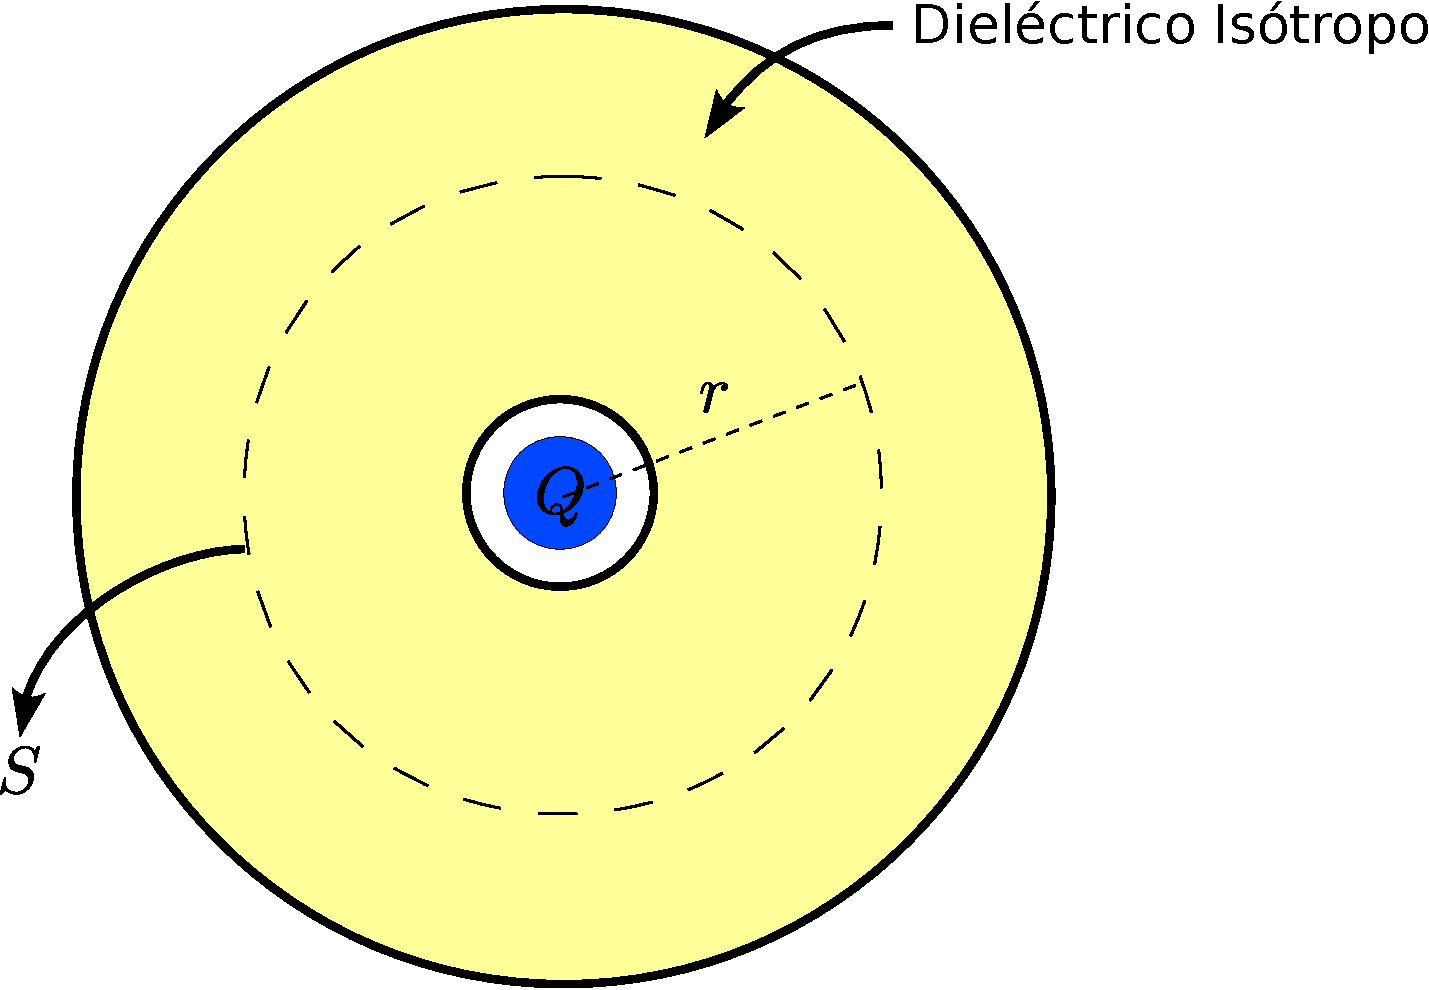
\psfig{file=fig/fig-dielectrico-y-carga-01.pdf,height=4cm,angle=0}}
\caption{Un material diel'ectrico is'otropo con una carga central.}
\label{diel02}
\end{figure}
Consideremos una carga (externa) $Q$ situada en el centro de una
esfera diel'ectrica \textit{is'otropa}, ver figura \ref{diel02}, podemos encontrar el vector de desplazamiento aplicando (\ref{GaussD}). Debido a la simetr'ia del sistema (ya que asumimos que el diel'ectrico es \textit{is'otropo}, ver secciones \ref{sec:aniso} y \ref{sec:iso}), tendremos que $\vec{D}(\vec{x})=D(r)\hat{r}$. Eligiendo una superficie Gaussiana esf'erica de radio $r$ centrada en la carga $Q$, encontramos entonces que
\begin{equation}
 D(r)\oint_S dS=D(r)4\pi r^2=Q,
\end{equation}
y por lo tanto
\begin{equation}
 \vec{D}(\vec{x})=\frac{Q}{4\pi}\frac{1}{r^2}\,\hat{r}.
\end{equation}


\subsection{Relaci'on Constitutiva, susceptibilidad, permeabilidad}

Cada medio se caracteriza por la polarizaci'on $\vec{P}(\vec{x})$ que presenta,
dados los campos/cargas externas. Esta polarizaci'on $\vec{P}(\vec{x})$ depende
entonces de los campos/cargas externas y de la constituci'on at'omica/molecular
del material (y en principio de otras propiedades, como la temperatura,
presi'on, etc). 
%Equivalentemente, esta informaci'on acerca de las propiedades
%del material puede expresarse en la relaci'on entre el campo el'ectrico
%$\vec{E}(\vec{x})$ y el vector desplazamiento el'ectrico $\vec{D}(\vec{x})$.

En un elemento de volumen dado del medio 'este modificar'a su distribuci'on microsc'opica de cargas como respuesta al campo el'ectrico ``total"\,que act'ua sobre este elemento, hasta finalmente adoptar un cierta polarizaci'on. Podemos, por tanto, considerar que $\vec{P}=\vec{P}(\vec{E})$ o, equivalentemente
$\vec{D}=\vec{D}(\vec{E})$. Esta 'ultima relaci'on es llamada
\textit{relaci'on constitutiva} del medio. El problema es que el campo
$\vec{E}(\vec{x})$ en un punto dado (con vector de polarizaci'on $\vec{P}(\vec{x})$ y
por tanto desplazamiento $\vec{D}(\vec{x})$) depende tambi'en de c'omo se
polariza el medio \textit{en otras regiones}, e.d., $\vec{E}(\vec{x})$ depende
en general de\footnote{Matem'aticamente, esto significa que, en
general, $\vec{E}$ es un \textit{funcional}, una ``funci'on de funciones''\, o
una ``funci'on no-local''\, de $\vec{P}$.} $\vec{P}(\vec{x}')$.
En otras palabras, en general la polarizaci'on que se presentar'a en un medio es fruto de la  \textit{respuesta colectiva} del material a los campos externos.

 Vemos entonces que calcular $\vec{P}(\vec{x})$ desde ``primeros principios'' es en gerenal dif'icil y requiere conocer los detalles de la estructura del material en estudio.

Existe una gran variedad de medios materiales con propiedades el'ectricas
diferentes e interesantes. Existen por ejemplo medios que tienen \textit{polarizaci'on
no nula a'un en ausencia de campos/cargas externas}. Estos medios son conocidos
como \textit{electretos} (an'alogos el'ectricos de los im'anes permanentes), y 
\textit{ferroel'ectricos} (que presentan polarizaci'on no nula bajo una cierta
temperatura cr'itica, de Curie, an'alogamente a los ferromagnetos). Un ejemplo
de material ferroel'ectrico es el $BaTiO_3$ (titanato de bario), que exhibe un
momento dipolar el'ectrico no nulo a temperaturas bajo $120^{\rm o}\,C$. Un ejemplo de electreto es el cuarzo ($SiO_2$, di'oxido de Silicio), que presenta \textit{propiedades piezoel'ectricas}.

Es 'util adem'as distinguir entre distintos tipos de polarizaci'on, dependiendo del mecanismo que gobierne dicha propiedad: \textit{polarizaci'on electr'onica}, p.ej. cuando un 'atomo se ``deforma"\,en presencia de un campo externo; \textit{polarizaci'on i'onica}, causada por arreglo de iones (p.ej. $NaCl$); \textit{polarizaci'on polar} que se manifiesta en los gases (cuando la
temperatura aumenta, disminuye la polarizaci'on porque las mol'eculas se
``desordenan").

M'as a'un, en algunos materiales (``no-lineales''\,) la respuesta
(polarizaci'on) del material puede depender no-linealmente del campo el'ectrico.

Sin embargo, existe una gran variedad de materiales que, desde el punto de
vista macrosc'opico, pueden ser modelados adecuadamente (es decir, con \textit{precisi'on suficiente} en la mayor'ia de las situaciones) por una relaci'on lineal entre $\vec{D}$ y $\vec{E}$. Un \textit{material lineal}, pero en general \textit{no-local}, puede describirse a
trav'es de una relaci'on de la forma
\begin{equation}
D_i[\vec{E}](\vec{x},t)=\int
f_{ij}(\vec{x},\vec{x}',t,t')\,{E}_j(\vec{x}',t')\,dV' dt',
\end{equation}
donde $f_{ij}(\vec{x},\vec{x}',t,t')$ es un cierto tensor que describe las
propiedades del medio. Como la polarizaci'on y por tanto el vector
desplazamiento en un punto $\vec{x}$ del medio est'an influenciadas en forma
m'as determinante por lo que le ocurre al material en la inmediata vecindad de
$\vec{x}$ es de esperar que la funci'on $f_{ij}(\vec{x},\vec{x}',t,t')$ sea
concentrada en torno a $\vec{x}$, es decir, que decaiga r'apidamente para
$|\vec{x}'-\vec{x}|\gg d$ donde $d$ es la escala caracter'istica de la
estructura microsc'opica del medio.

Por otro lado, existen muchos casos en que es \textit{suficiente} considerar una
\textit{relaci'on constitutiva local} en la que el vector desplazamiento en un
punto dado puede modelarse como dependiendo exclusivamente del valor del campo
el'ectrico \textit{en el mismo punto} (macrosc'opico), es decir
$\vec{D}(\vec{x})=\vec{D}(\vec{E}(\vec{x}))$ o, equivalentemente
$\vec{P}(\vec{x})=\vec{P}(\vec{E}(\vec{x}))$.

En un material descrito por una relaci'on constitutiva local podemos considerar
la dependencia de $\vec{P}$ con $\vec{E}$ a trav'es de una expansi'on en serie
de la forma:
\begin{equation}\label{expP}
P_i(x)=P_i(E_j(x))=(P_i)_{\vec{E}=\vec{0}}
+E_j(\partial_jP_i)_{\vec{E}=\vec{0}}+\frac{1}{2}
E_jE_k(\partial_j\partial_k P_i)_{\vec{E}=\vec{0}}+\cdots,
\end{equation}
que esperamos sea 'util para campos el'ectricos suficientemente d'ebiles (en el
presente contexto s'olo podemos saber \textit{a posteriori} qu'e tan d'ebil
requiere ser el campo). Note que en el lado derecho de (\ref{expP}) las derivadas $\partial_i$ denotan derivadas respecto a la componente $i$-'esima del campo el'ectrico, es decir $\partial_iP_j={\partial P_j}/{\partial E_i}$, etc.. Las cantidades $(P_i)_{\vec{E}=\vec{0}}$,
$(\partial_jP_i)_{\vec{E}=\vec{0}}$,
$(\partial_j\partial_k P_i)_{\vec{E}=\vec{0}}$, etc. son
tensores (cartesianos) que asumen diferentes valores para cada material y pueden ser
considerados como par'ametros (a determinar). Con esto, podemos escribir
\begin{equation}
\boxed{P_i(x)={\cal A}_i+{\cal A}_{ij}E_j+{\cal A}_{ijk}
E_jE_k+\cdots.}
\end{equation}
En general, si el material es \textit{inhomog'eneo} (por ejempo, si est'a formado por
capas de distintos materiales), los tensores ${\cal A}_i$, ${\cal A}_{ij}$, ${\cal A}_{ijk}$, etc. depender'an de la posici'on. Para materiales no-ferroel'ectricos (la gran mayor'ia) tenemos que ${\cal A}_i=0$.



\subsection{Medios lineales anis'otropos}\label{sec:aniso}

Adicionalmente, si la polarizaci'on de un material es descrita apropiadamente
por una relaci'on lineal, como ocurre en el caso de campos el'ectricos
suficientemente d'ebiles, tendremos
\begin{equation}
\boxed{P_i(x)=\varepsilon_0\chi_{ij}(x)E_j(x),} \label{rcml}
\end{equation}
entonces decimos que el medio es \textit{lineal}. El tensor $\chi_{ij}$ es
llamado \textit{tensor de susceptibilidad el'ectrica} del medio.  El factor $\varepsilon_0$ es incluido de modo que $\chi_{ij}$ es un tensor adimensional. En este caso,
usando (\ref{defD}) y (\ref{rcml}), tenemos que
\begin{equation}\label{rclai}
\boxed{D_i(x)=\varepsilon_{ij}(x)E_j(x)=\varepsilon_0\,\kappa_{ij}(x)E_j(x),}
\end{equation}
donde hemos definido el \textit{tensor de permitividad} del medio
$\varepsilon_{ij}$, por
\begin{equation}
\varepsilon_{ij}:=\varepsilon_0(\delta_{ij}+\chi_{ij})
\end{equation}
y, alternativamente,  el \textit{tensor diel'ectrico},
\begin{equation}
\kappa_{ij}:=\frac{1}{\varepsilon_0}\varepsilon_{ij}=\delta_{ij}+\chi_{ij},
\end{equation}
que tiene la ventaja de ser una cantidad adimensional.

Es posible probar por
argumentos energ'eticos que si el medio no es disipativo (no existen mecanismos
de transferencia de energ'ia del campo el'ectrico a otras formas de energ'ia)
entonces necesariamente $\chi_{ij}$ (y por tanto $\varepsilon_{ij}$ y
$\kappa_{ij}$) es un tensor \textit{sim'etrico} y que posee, por lo
tanto, 6 componentes independientes. La descripci'on de las
propiedades de un medio lineal a trav'es de un tensor de susceptibilidad
el'ectrica incluye el caso en que el medio sea \textit{anis'otropo}, es decir,
que sus propiedades no sean invariantes bajo rotaciones o, en otras palabras,
que posea ciertas \textit{direcciones preferentes}. En un medio anis'otropo, la
polarizaci'on no ser'a en general paralela al campo el'ectrico (excepto para las
direcciones preferentes dadas por las direcciones principales. Ver secci'on
\ref{secDP}.), esto como
resultado de la estructura microsc'opica del material (t'ipicamente, cristales),
que tienen como consecuencia que el material se polarize en algunas direcciones
m'as f'acilmente que en otras.


Note que en el caso m'as general en que se consideran campos el'ectricos dependientes del tiempo (esto es necesario, por ejemplo, en el caso de propagaci'on de ondas electromagn'eticas), a'un cuando un medio pueda considerarse lineal y local respecto a su dependencia con la posici'on, la relaci'on constitutiva es de la forma
\begin{equation}
D_i(x,t)=\int f_{ij}(t,t')E_j(x,t')\,dt'.
\end{equation}
En estos casos es conveniente considerar las \textit{transformadas de Fourier temporal} de los campos, es decir $\tilde{D}_i(x,\omega)$, $\tilde{E}_i(x,\omega)$, etc., ya que permiten escribir la relaci'on constitutiva como
\begin{equation}\label{RELtilde}
\tilde{D}_i(x,\omega)=\tilde{\varepsilon}_{ij}(x,\omega)\tilde{E}_j(x,\omega). 
\end{equation}
Comparando \eqref{RELtilde} con \eqref{rclai} vemos que en el caso m'as general, el tensor $\tilde{\varepsilon}_{ij}(x,\omega)$ juega un rol an'alogo a $\varepsilon_{ij}$ en \eqref{rclai} y tambi'en es llamado, por esta raz'on, el tensor diel'ectrico del medio. Note, sin embargo, que este tensor \textit{asume valores complejos y depende en general de la frecuencia} $\omega$.


\subsection{Medios lineales is'otropos}\label{sec:iso}
Si el material es is'otropo, es decir, si 'este no posee ninguna direcci'on
preferente, la polarizaci'on debe necesariamente ser paralela al campo
el'ectrico, independientemente de la direcci'on de este 'ultimo. Esta condici'on requiere que el tensor de susceptibilidad sea proporcional al tensor identidad,
\begin{equation}
\chi_{ij}=\chi\,\delta_{ij},
\end{equation}
de modo que
\begin{equation}
\vec{P}=\varepsilon_0\chi\vec{E}.
\end{equation}
Muchos materiales presentan propiedades de polarizaci'on independientes de
la direcci'on del campo el'ectrico, es decir, son is'otropos. Por ejemplo, los
gases, l'iquidos (excepto los, as'i llamados, \textit{cristales liquidos}), s'olidos amorfos (pl'asticos, vidrio).
Los medios no-lineales, pero is'otropos, pueden ser descritos usando
$\vec{P}=\varepsilon_0\chi(|\vec{E}|)\vec{E}$.

En este curso, a menos que se explicite lo contrario, consideramos siempre
materiales lineales, is'otropos y homog'eneos. En este caso, es suficiente
introducir la (``constante de''\,) permitividad y/o la constante diel'ectrica
por
\begin{equation}
\varepsilon:=\varepsilon_0(1+\chi), \qquad
\kappa:=\frac{\varepsilon}{\varepsilon_0}=1+\chi.
\end{equation}
Note que en un medio polarizable es de esperar que $\chi>0$, de modo que
$\varepsilon>\varepsilon_0$ o, equivalentemente, $\kappa>1$. El vac'io puede ser
considerado como un ``medio is'otropo''\, con $\chi=0$ y $\kappa=1$, es decir, no polarizable.
Recuerde tambi'en que el 'indice de refracci'on de la mayor'ia de los medios
(``no-magn'eticos''\,) es dado por $n\approx\sqrt{\kappa}$.
\begin{table}[!h]
\begin{center}
\begin{tabular}{c|c}
Material &   $\kappa$ \\ \hline\hline
Vac'io & 1 \\
Aire (seco, $0^{\rm o}$C, 1 bar)  & 1,00059 \\
Agua ($110^{\rm o}$C, 1 bar)  & 1,0126 \\
Agua ($20^{\rm o}$C) &  80,0 \\
Hielo ($-30^{\rm o}$C) &  99 \\
$SrTiO_3$ (cristal, $10$K)  & 12.000 \\
\end{tabular}
\caption{Algunos materiales is'otropos y sus constantes diel'ectricas.}
\end{center}
\end{table}

\subsection{Ecuaci'on de Poisson y su generalizaci'on}

Usando (\ref{divD}) y (\ref{E=nablaphi}) encontramos la generalizaci'on de la
ecuaci'on de Poisson para el potencial en un diel'ectrico lineal y local:
\begin{equation}
 \boxed{\partial_i\left(\kappa_{ij}\,\partial_j \phi\right)
=-\frac{1}{\varepsilon_0}\rho_{\rm ext}.}
\end{equation}
Para un material homog'eneo e is'otropo, esta ecuaci'on se reduce a
\begin{equation}\label{Poissond}
 \boxed{\nabla^2\phi=-\frac{1}{\varepsilon}\rho_{\rm ext},}
\end{equation}
que tiene la misma forma (matem'aticamente, es la \textit{misma} ecuaci'on) que
en caso del campo en el vac'io ($\varepsilon=\varepsilon_0$). Finalmente, en
regiones fuera de cargas externas (!`\,pero \textit{no} de cargas de
polarizaci'on!), el potencial satisface la ecuaci'on de Laplace. Como
consecuencia, es posible usar las t'ecnicas conocidas para solucionar esta ecuaci'on, por ejemplo, expansi'on en funciones especiales, o funciones de Green, en el caso de los diel'ectricos.
Como veremos a continuaci'on, una diferencia importante respecto al caso en el
vac'io ser'a la implementaci'on de las condiciones de borde o frontera.


\subsection{Direcciones principales de un medio anis'otropo}\label{secDP}

Como vimos, en un medio anis'otropo, el campo el'ectrico no tiene en general
la misma direcci'on que el vector desplazamiento.
Existen, sin embargo, direcciones ``especiales''\, a lo largo de las cuales el
campo el'ectrico s'i tiene la misma direcci'on que la polarizaci'on. Esto significa
que, si $\hat{n}$ es una de estas direcciones, conocidas como \textit{direcciones
principales} del material, entonces $\vec{E}=E\hat{n}$ y $\vec{D}=D\hat{n}$.
Insertando estas condiciones en (\ref{rclai}) obtenemos que
\begin{equation}
\kappa_{ij}\,\hat{n}_j= \lambda\,\hat{n}_i, \qquad D=\varepsilon_0\lambda E.
\end{equation}
Vemos de aqu'i que las direcciones principales corresponden a los vectores
propios de la matriz  $\kappa_{ij}$, mientras que el valor propio $\lambda$ es
el valor de la constante diel'ectrica del material a lo largo de aquella
direcci'on principal. Como la matriz $\kappa_{ij}$ es real y sim'etrica, es
posible encontrar tres vectores propios ortonormales, es decir, una base
ortonormal formada por las direcciones principales del material. Existen
distintos casos particulares e interesantes de materiales anis'otropos
correspondiendo a si los valores propios son todos diferentes o iguales. Si
todos los valores propios son iguales, el material es is'otropo, puesto que en
ese caso $\kappa_{ij}=\lambda\,\delta_{ij}$. Si dos valores propios son iguales
y uno diferente, se dice que el material es \textit{uniaxial} (puesto que
tienen una direcci'on distintiva, aquella descrita por el vector propio del
valor propio distinto a los otros dos. Esta direcci'on es llamada \textit{eje
'optico}). Un ejemplo de material uniaxial natural es la Calcita ($CaCO_3$). En
materiales uniaxiales la propagaci'on de la luz presenta el fen'omeno llamado
\textit{birefringencia}, en los que la luz en su interior se propaga, en
general, por dos trayectorias diferentes (rayo ``ordinario''\, y
``extraordinario'') correspondientes a dos 'indices de refracci'on diferentes.
Adem'as, es posible inducir anisotrop'ia (y por tanto, en general,
birefringencia), comprimiendo un material en una direcci'on dada, o
con un campo el'ectrico intenso externo (\textit{efecto Kerr}). Finalmente, si
los tres valores propios del tensor diel'ectrico son diferentes, entonces el
material (t'ipicamente un cristal) es llamado \textit{biaxial}.

\begin{table}[!h]
\begin{center}
\begin{tabular}{l c |c| c}
Mineral 		& 	F'ormula qu'imica 	&	$n_{\rm o}=\sqrt{\kappa_\perp}$	& 	$n_{\rm e}=\sqrt{\kappa_\parallel}$
%& 	 $\Delta n=n_e-n_o$
\\
\hline\hline
Berilo 			& Be$_3$Al$_2$(Si6O18)	&	1.602	& 	1.557	
%&	-0.045	
\\
Calcita 		&	CaCO$_3$  	&	1.658	& 	1.486	
%& 	-0.172	
\\
%Calomelano 		&	Hg$_2$Cl$_2$	& 	1.973	& 	2.656	
%& 	+0.683	
%\\
%cinnabar 		&	HgS    		&	2.905	& 	3.256	
%& 	+0.351	
%\\
Hematita 		&	Fe$_2$O$_3$	&	2.940	& 	3.220	
%& 	+0.287	
\\
Hielo 			&	H$_2$O 		&	1.309	&	1.313	
%& 	+0.014	
\\
Niobiato de litio 	&	LiNbO$_3$	&	2.272	& 	2.187	
%& 	-0.085	
\\
Fluoruro de magnesio 	&	MgF$_2$		&	1.380	& 	1.385	
%& 	+0.006	
\\
Quarzo 			&	SiO$_2$		&	1.544	& 	1.553	
%& 	+0.009	
\\
Rub'i 			& Al$_2$O$_3$:Cr	&	1.770 	&	1.762	
%& 	-0.008	
\\
%Rutilo 			&	TiO$_2$ 		&	2.616	& 	2.903	
%& 	+0.287	
%\\
%Peridot 		&	  		&	1.690	& 	1.654	
%& 	-0.036	
%\\
Zafiro	 		&	Al$_2$O$_3$	&	1.768	& 	1.760	
%& 	-0.008	
\\
Nitrato de sodio	&	NaNO$_3$	&	1.587	& 	1.336	
%& 	-0.251	
%\\
%Turmalina 		&	  		&	1.669	& 	1.638	
%& 	-0.031	
\\
Circ'on, high 		&	ZrSiO$_4$	&	1.920 -1.960	&  1.967-2.015	
%& +0.047; +0.055	
\end{tabular}
\caption{Algunos cristales uniaxiales y sus 'indices de refracci'on. Datos tabulados para $\lambda\sim 590\,{\rm [nm]}$ \cite{hyper}.}
\end{center}
\end{table}

\begin{table}[!h]
\begin{center}
\begin{tabular}{l c |c|c|c}
Mineral			& F'ormula qu'imica		& $\sqrt{\kappa_x}$	&	$\sqrt{\kappa_y}$	&  $\sqrt{\kappa_z}$	\\
\hline\hline
B'orax 	 		&Na$_2$B$_4$O$_7$·10H$_2$O& 	1.447	& 	1.469	& 	1.472	\\
Sulfato de magnesio		&  MgSO$_4$·7(H$_2$O)	& 	1.433	& 	1.455	& 	1.461	\\
%Biotita		&			&  	1.595	& 	1.640	& 	1.640	\\
%Moscovita		&			&  	1.563	& 	1.596	& 	1.601	\\
Olivina			& 	(Mg,Fe)2SiO	& 	1.640	& 	1.660	& 	1.680	\\
Perovskita		& 	CaTiO$_3$	& 	2.300	& 	2.340	& 	2.380	%\\
%Topacio			&			&  	1.618	& 	1.620	& 	1.627	\\
%Ulexita			&			&  	1.490	& 	1.510	& 	1.520	
\end{tabular}
\caption{Algunos cristales biaxiales. Datos tabulados para $\lambda\sim 590\,{\rm [nm]}$ \cite{hyper}.}
\end{center}
\end{table}
\subsection{Condiciones de frontera para $\vec{D}$}

El vector desplazamiento el'ectrico satisface la ecuaci'on (\ref{divD}), que es
de la misma forma que la ley de Gauss (\ref{leygauss-dif}), con la diferencia
que en (\ref{divD}) el factor $\varepsilon_0$ est'a ausente y que la densidad de carga en el lado derecho es s'olo la densidad de cargas externas (\underline{no} las de polarizaci'on). Como consecuencia, podemos aplicar el mismo procedimiento discutido en la secci'on \ref{secCBE} para derivar las condiciones que el vector desplazamiento debe satisfacer en la frontera de dos materiales. Consideramos una superficie que divide dos diel'ectricos de propiedades diferentes, en la que, eventualmente, existe una densidad de carga externa $\sigma_{\rm ext}$. Si $\hat{n}$ es el vector unitario normal a la superficie en un punto dado, que apunta desde el material 1 hasta el 2, entonces
\begin{figure}[!h]
\centerline{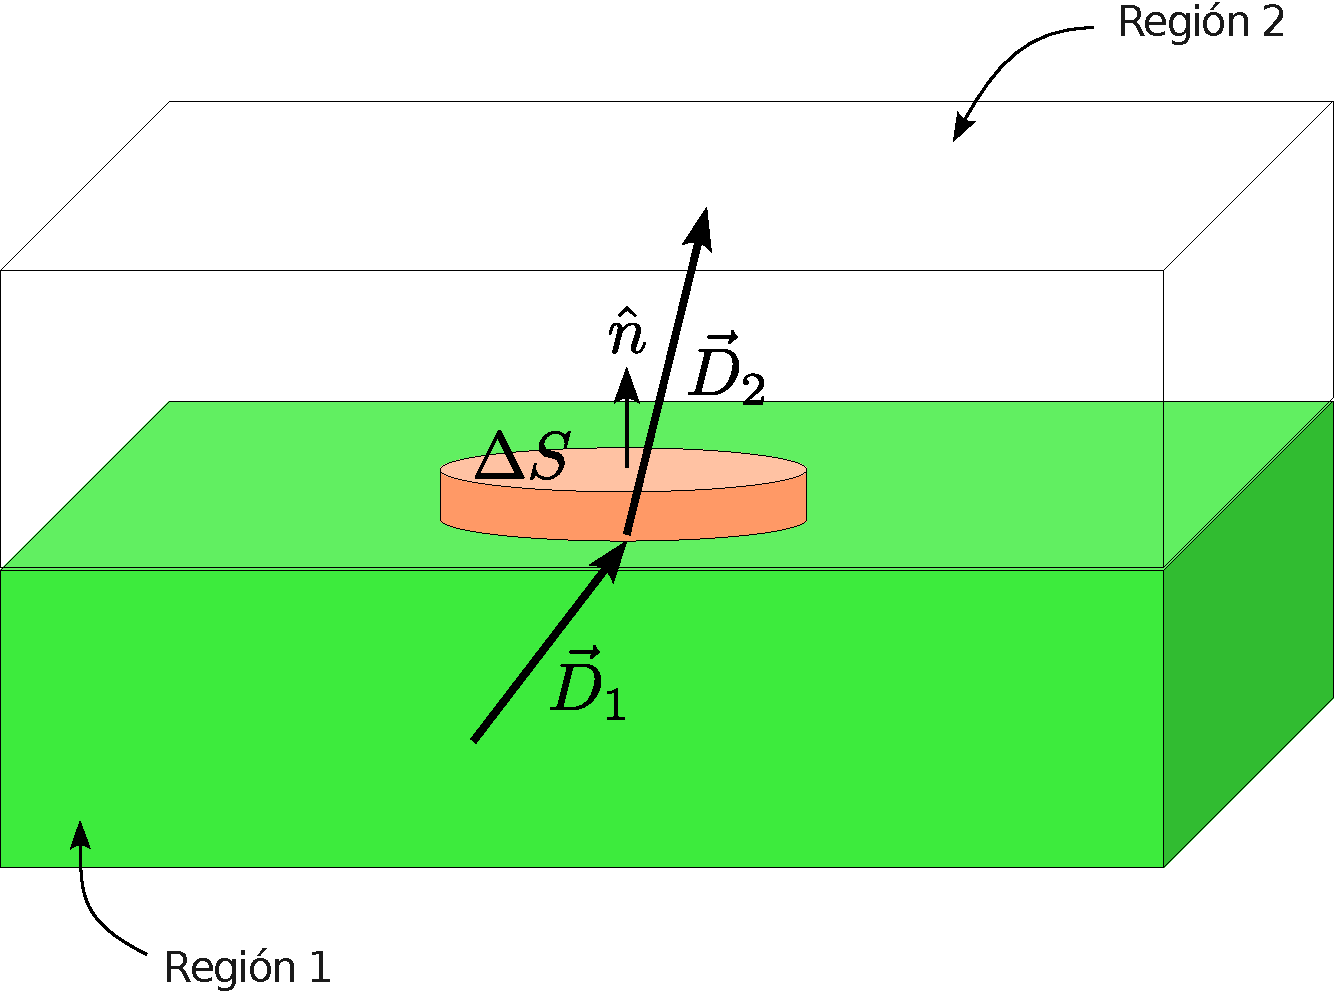
\psfig{file=fig/fig-dielectrico-condicion-borde-01.pdf,height=5cm,
angle=0}}
\caption{La componente normal del vector desplazamiento puede ser discontinua
si existen cargas externas en el la interfase entre dos diel'ectrico.}
\label{CF1}
\end{figure}
\begin{equation}\label{saltoDn}
\boxed{\vec{D_2}\cdot\hat{n}-\vec{D_1}\cdot\hat{n}=\sigma_{\rm
ext}.}
\end{equation}

Por otro lado, el campo el'ectrico $\vec{E}$ sigue satisfaciendo (\ref{rotE0}),
de modo que, como consecuencia, su componente tangencial es continua a trav'es
de la superficie, tal como lo expresa la condici'on (\ref{Etconst}). Recuerde
finalmente que el potencial el'ectrico siempre es una funci'on continua, de
modo que el campo el'ectrico, aunque eventualmente discontinuo, es finito en
todo punto.
\begin{figure}[!h]
\centerline{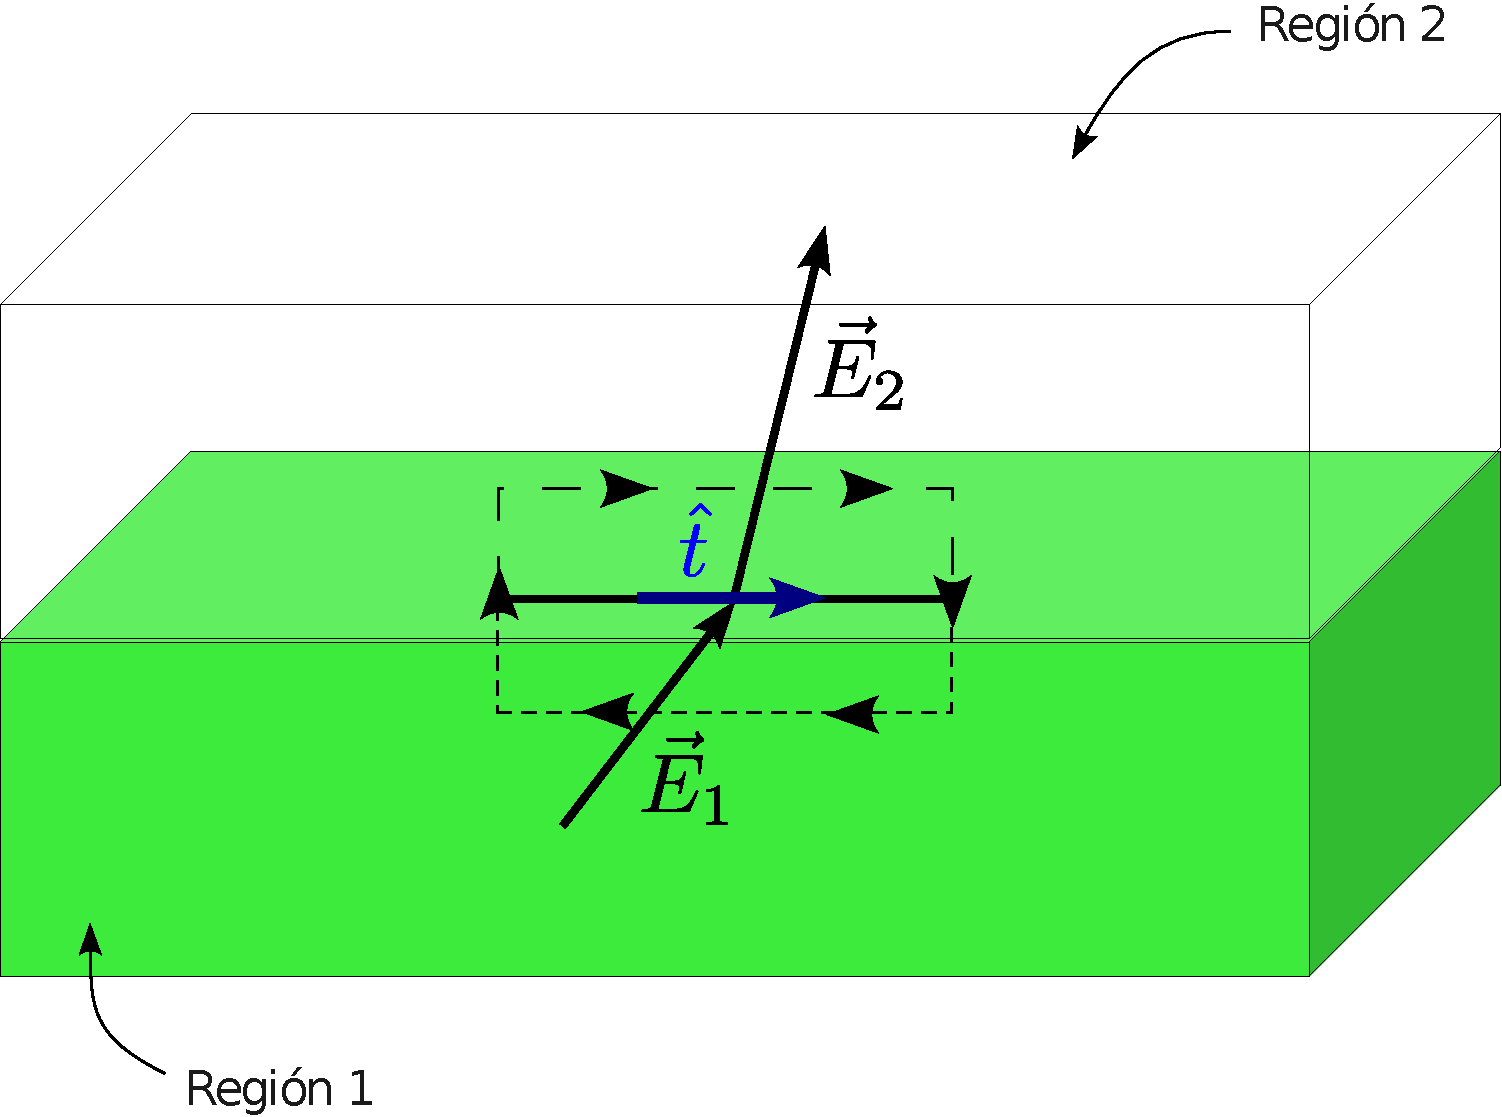
\psfig{file=fig/fig-dielectrico-condicion-borde-02.pdf,height=5cm,
angle=0}}
\caption{La componente tangencial del campo el'ectrico es siempre continua
en una interfase.}
\label{CF2}
\end{figure}

\subsection{Caso de un medio lineal e is'otropo}

Consideramos aqu'i el caso particular de medios lineales e is'otropos caracterizados por las constantes diel'ectricas $\kappa_1$ y $\kappa_2$ respectivamente. Consideramos adem'as el 'angulo entre los vectores campo el'ectrico a cada lado de la superficie y el vector normal. Ver figura \ref{CF3}. 
\begin{figure}[!h]
\centerline{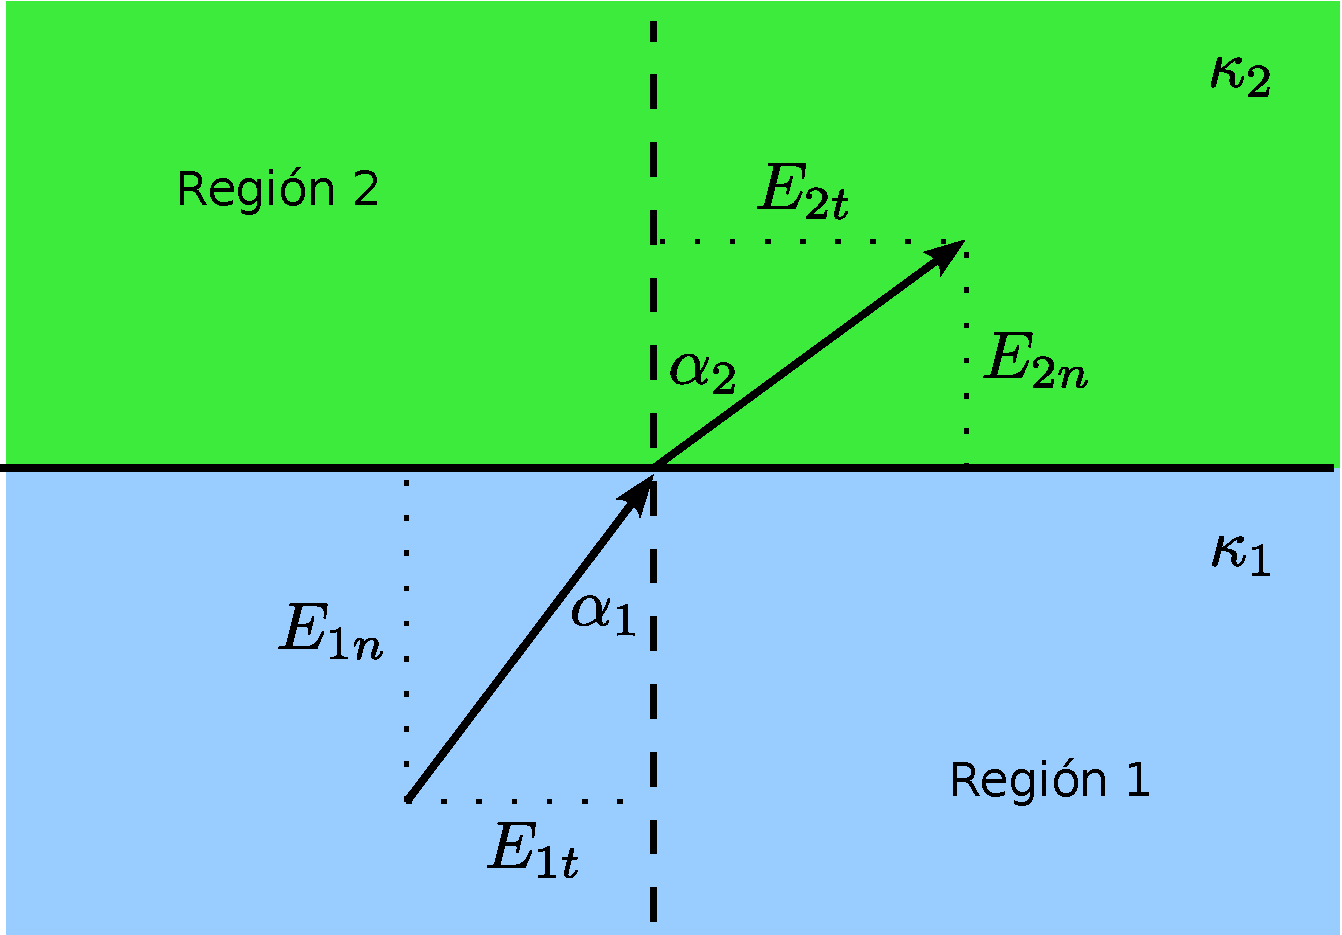
\psfig{file=fig/fig-dielectrico-condicion-borde-03.pdf,height=5cm,
angle=0}}
\caption{Refracci'on de las l'ineas de campo.}
\label{CF3}
\end{figure}
Aqu'i tendremos que, en ausencia de cargas externas, la componente normal del vector desplazamiento es continua a trav'es de la superficie,  $\vec{D}_1\cdot\hat{n}=\vec{D}_2\cdot\hat{n}$, que puede escribirse m'as expl'icitamente como:
\begin{equation}\label{Enid}
\kappa_1 E_1\cos\alpha_1=\kappa_2E_2\cos\alpha_2.
\end{equation}
Por otro lado, la condici'on sobre la componente tangencial a la superficie implica que
\begin{equation} \label{Etid}
 E_1\sin\alpha_1=E_2\sin\alpha_2.
\end{equation}
Dividiendo (\ref{Etid}) por (\ref{Enid}) (asumiendo naturalmente que $E_1$ y $E_2$ son no nulos), obtenemos una simple relaci'on entre los 'angulos $\alpha_1$ y $\alpha_2$:
\begin{equation}
 \frac{\tan\alpha_1}{\kappa_1}=\frac{\tan\alpha_2}{\kappa_2}.
\end{equation}

\subsubsection{Ejemplo: Esf'era diel'ectrica en un campo el'ectrico externo uniforme}
Aqu'i consideraremos el ejemplo de una esfera diel'ectrica (lineal e is'otropa) de radio $R$ y constante diel'ectrica $\kappa_1$ sumergida en un medio de constante diel'ectrica $\kappa_2$ y en presencia de un campo externo constante $\vec{E}_0$.

En este caso no existen cargas externas en el dominio considerado (las 'unicas cargas externas del problema ser'ian aquellas que generan el campo externo, que consideraremos est'an ubicadas muy lejos de la esfera). Entonces el potencial el'ectrico, de acuerdo a (\ref{Poissond}), satisface la ecuaci'on de Laplace tando dentro ($r\le R$) como fuera ($r\ge R$) de la esfera. Resolveremos el problema en coordenadas esf'ericas orientando el eje $z$ en la direcci'on de $\vec{E}_0$. Entonces, debido a la simetr'ia del problema (recuerde que los medios son is'otropos) los campos tendr'an simetr'ia axial. En particular $\phi=\phi(r,\theta)$. Por esto, la forma general del campo en cada regi'on es
 \begin{equation}
 \phi(r,\theta)=\sum_{l=0}^{\infty}\left[  A_lr^{l}+B_lr^{-(l+1)}\right]
 P_l(\cos\theta).
 \end{equation}
En el interior de la esfera el potencial debe ser finito en todo punto y, en particular, en el origen $r=0$. Esta condici'on, junto con la elecci'on $\phi (r=0,\theta)\stackrel{!}{=}0$, reduce la forma posible del potencial a 
 \begin{equation}\label{phiint}
 \phi(r,\theta)=\sum_{l=1}^{\infty}A_l^{(1)}r^{l}P_l(\cos\theta), \qquad r\le R.
 \end{equation}
Por otro lado, lejos de la esfera ($r\gg R$) el campo el'ectrico debe tender al campo el'ectrico externo $\vec{E}_0=E_0\hat{z}$. Esto es equivalente a que el potencial satisfaga
\begin{equation}
 \phi(r,\theta)\to -E_0z+\alpha = -E_0\,r\cos\theta+\alpha, \qquad r\gg R,
\end{equation}
donde $\alpha$ es una constante. Con esta condici'on, el potencial fuera de la esfera s'olo puede adoptar la forma
\begin{equation}\label{phiext}
\phi(r,\theta)=\alpha-E_0\,r\cos\theta+\sum_{l=0}^{\infty}B_l^{(2)}
 r^{-(l+1)}P_l(\cos\theta), \qquad r>R.
\end{equation}
El potencial es una funci'on continua. Por lo tanto, en $r=R$ las soluciones internas y externas deben adoptar el mismo valor. Usando (\ref{phiint}) y (\ref{phiext}) encontramos as'i la condici'on
 \begin{equation}
 \sum_{l=1}^{\infty}A_l^{(1)}R^{l}P_l(\cos\theta)  
 =\alpha-E_0\,R\cos\theta+\sum_{l=0}^{\infty}B_l^{(2)}R^{-(l+1)} P_l(\cos\theta)
 \end{equation}
 que implica, para $l=0$, que
\begin{equation}\label{ecl0a}
\alpha-B_0^{(2)}R^{-1}=0.
\end{equation}
Adem'as, para $l=1$, obtenemos
\begin{equation}\label{ecl1a}
 A_1^{(1)}R =-E_0R+B_1^{(2)}R^{-2}.
\end{equation}
Finalmente, para $l\geq2$, encontramos
\begin{equation}\label{eclla}
 A_l^{(1)}R^{l} =B_l^{(2)}R^{-(l+1)}.
\end{equation}
Por otro lado, la condici'on (\ref{saltoDn}) se reduce, ya que $\sigma_{\rm ext}=0$, a $\vec{D}_1\cdot\hat{n}=\vec{D}_2\cdot\hat{n}$. Adem'as en este caso $\hat{n}=\hat{r}$, por lo que la condici'on es equivalente a
\begin{equation}
\kappa_1\left.\frac{\partial\phi}{\partial r}\right|_{r=R^-}
=\kappa_2\left.\frac{\partial\phi}{\partial r}\right|_{r=R^+}.
\end{equation}
Reemplazano nuevamente (\ref{phiint}) y (\ref{phiext}) en esta condici'on obtenemos
\begin{equation}\label{condD}
 k\sum_{l=1}^{\infty}A_l^{(1)}lR^{l-1}P_l(\cos\theta) =-E_0P_1(\cos\theta)  -\sum_{l=0}^{\infty}(l+1)B_l^{(2)}R^{-(l+2)}P_l(\cos\theta),
\end{equation}
donde hemos definido $k:=\kappa_1/\kappa_2$. Para $l=0$ esta condici'on implica que
\begin{equation}\label{ecl0b}
B_0^{(2)}=0.
\end{equation}
Para el caso $l=1$, obtenemos
\begin{equation}\label{ecl1b}
kA_1^{(1)}  =-E_0-2B_1^{(2)}R^{-3}.
\end{equation}
Finalmente, para $l\geq2$, encontramos la condici'on
\begin{equation}\label{ecllb}
klA_l^{(1)} =-(l+1)B_l^{(2)}R^{-(2l+1)}.
\end{equation}
Al reemplazar el resultado (\ref{ecl0b}) en (\ref{ecl0a}) obtenemos $\alpha=0$. Similarmente, las ecuaciones (\ref{ecl1a}) y (\ref{ecl1b}) permiten encontrar las constantes $A_1^{(1)}$ y $B_1^{(2)}$. Simple 'algebra muestra que la soluci'on en este caso es dada por
\begin{equation}
 A_1^{(1)}=\frac{-3}{k+2}E_0, \qquad, B_1^{(2)}=\frac{k-1}{k+2}R^3E_0.
 \end{equation}
Finalmente, las ecuaciones (\ref{eclla}) y (\ref{ecllb}) determinan $A_l^{(1)}$ y $B_l^{(2)}$ para $l\ge 2$. En este caso, sin embargo, la 'unica soluci'on posible es la nula, es decir,
\begin{equation}
A_l^{(1)}=0, \qquad B_l^{(2)}=0, \qquad l\ge 2.
\end{equation}
Con esto, la soluci'on para el potencial queda totalmente determinado tanto dentro como fuera de la esfera:
\begin{equation}
\phi(r,\theta)=\frac{-3\kappa_2}{\kappa_1+2\kappa_2}E_0\,r\cos\theta, \qquad r\le R
\end{equation}
y
\begin{equation}
\phi(r,\theta)=-E_0\,r\cos\theta +\frac{\kappa_1-\kappa_2}{\kappa_1+2\kappa_2}R^3E_0 \frac{\cos\theta}{r^2}, \qquad r\ge R.
\end{equation}
 
 Ahora estudiaremos algunas caracter'isticas de la soluci'on obtenida, en el caso particular en que fuera de la esfera hay s'olo vac'io, es decir, $\kappa_2=1$. Primero, el potencial en el interior de la esfera puede escribirse, en coordenadas cartesianas como
 \begin{equation}
\phi(r,\theta)=\frac{-3}{\kappa_1+2}E_0\,z, \qquad r\le R,
\end{equation}
lo que implica que el campo el'ectrico en el interior de la esfera es homog'eneo y dado por
\begin{equation}
\vec{E}=\frac{3}{\kappa_1+2}\,\vec{E}_0, \qquad r\le R.
\end{equation}
% Adem'as,%
% \begin{equation}
% E_{r}^{(2)}=-\frac{\partial\phi^{(2)}}{\partial r}=E^0r\cos\theta
% +2\frac{k_1-k_2}{k_1+2k_2}a^3E^0r^{-2}\cos\theta
% \end{equation}%
% \begin{equation}
% E_{\theta}^{(2)}=-\frac{1}{r}\frac{\partial\phi^{(2)}}{\partial\theta
% }=-E^0r\sen\theta+\frac{k_1-k_2}{k_1+2k_2}a^3E^0r^{-2}%
% \sen\theta
% \end{equation}%
% \begin{equation}
% E_{\varphi}^{(2)}=0
% \end{equation}

Por otro lado, fuera de la esfera, el potencial consta de dos t'erminos: uno que corresponde al campo homog'eneo externo y otro con la forma (es decir, dependencia espacial) de un \textit{campo dipolar}. En efecto, el campo de un dipolo el'ectrico con momento dipolar $\vec{p}=p\hat{z}$ orientado a lo largo del eje $z$ es
 \begin{equation}
 \phi_{\rm dip}=\frac{p}{4\pi\varepsilon_0}\frac{\cos\theta}{r^2}.
 \end{equation}
Por lo tanto, el campo en el exterior de la esfera diel'ectrica es dado por la suma del campo externo$\vec{E}_0$ y el campo de un dipolo con momento dipolar
 \begin{equation}
\vec{p}=4\pi\varepsilon_0\frac{\kappa_1-1}{\kappa_1+2}R^3\,\vec{E}_0.
 \end{equation}
Puede verficarse que esta identificaci'on es correcta recordando que el vector de polarizaci'on es definido como la densidad de momento dipolar del medio. Como consecuencia, la relaci'on (\ref{pintPdV}) permite calcular el momento dipolar total de la esfera como una integral de volumen de su vector de polarizaci'on. En el caso estudiado, el vector de polarizaci'on es proporcional al campo el'ectrico y por lo tanto tambi'en homog'eneo al interior de la esfera:
\begin{align}
\vec{P} &= \varepsilon_0(\kappa_1-1)\vec{E} \\
&= \frac{3\varepsilon_0(\kappa_1-1)}{\kappa_1+2}\,\vec{E}_0.
\end{align}
Con esto, el momento dipolar de la esfera puede ser calculado f'acilmente:
\begin{align}
\vec{p} &= \int_V \vec{P}\,dV \\
&= \vec{P}\,V \\
&= \frac{3\varepsilon_0(\kappa_1-1)}{\kappa_1+2}\,\vec{E}_0\cdot \frac{4\pi}{3}R^3.
\end{align}
Finalmente, podemos calcular las densidades de carga de polarizaci'on en la esfera. Ya que el vector de polarizaci'on es homog'eneo, la densidad $\rho_P=0$. La densidad superficial de carga de polarizaci'on $\sigma_P$ es no nula:
\begin{align}
\sigma_P &= \vec{P}\cdot\hat{r}\\
&= \frac{3\varepsilon_0(\kappa_1-1)}{\kappa_1+2}\,E_0\,\cos\theta.
\end{align}

Finalmente, es interesante notar que el caso de un \textit{conductor} esf'erico de carga total nula, en un campo externo homog'eneo, ver secci'on \ref{sec:esfcond}, puede ser recobrado en el l'imite $\kappa_1\to\infty$.

\subsection{Modelos microsc'opicos simples de polarizaci'on}
\subsubsection{Polarizalibidad}
En muchos casos, los 'atomos que constituyen un diel'ectrico no est'an polarizados...

\subsection{Energ'ia electrost'atica en un diel'ectrico}

En la secci'on \ref{ed3_1_2} vimos una expresi'on para la energ'ia almacenada
en un campo dado o, equivalentemente la energ'ia necesaria para formar el
sistema de cargas correspondientes a un campo. Ahora calcularemos algo
an'alogo, pero diferente: la energ'ia almacenada en una configuraci'on de campo
en un sistema que consta de cargas externas y un diel'ectrico \underline{dado}.
En otras palabras, \textit{no incluiremos la energ'ia necesaria para formar el
diel'ectrico}, sino s'olo la energ'ia necesaria para montar una cierta
distribuci'on de cargas externas en un diel'ectrico preexistente.

El trabajo necesario para aumentar (en general, para cambiar) la densidad de
cargas externas en $\delta\rho_{\rm ext}(x)$ en un medio con potencial
$\phi(x)$ es dado por
\begin{equation}\label{Wdiel1}
 \boxed{\delta U=\int_{R^3}\phi(x)\delta\rho_{\rm ext}(x)\,dV.} 
\end{equation}
Usando (\ref{divD}) encontramos que el cambio en densidad de cargas externas
est'a relacionado con el cambio en el vector desplazamiento por medio de
$\vec\nabla\cdot(\delta\vec{D})=\delta\rho_{\rm ext}$. Usando esto, e integrando
por partes, podemos reescribir (\ref{Wdiel1}) como:
\begin{equation}
 \delta U=\oint_{\infty}\phi (x)\delta\vec{D}(x)\cdot
d\vec{S}+\int_{R^3}\vec{E}\cdot\delta\vec{D}\,dV.
\end{equation}
Asumiendo, como es usual, que los campos se anulan suficientemente r'apido en
el infinito, llegamos a
\begin{equation}
 \boxed{\delta U=\int_{R^3}\vec{E}(x)\cdot\delta\vec{D}(x)\,dV.} \label{dUE}
\end{equation}
Si las cargas externas est'an posicionadas de forma tal que (en cada punto) su
densidad es una fracci'on $\lambda$ de la densidad final, es decir, si es
$\lambda\rho_{\rm ext}(x)$, entonces el vector desplazamiento correspondiente
ser'a $\lambda\vec{D}(x)$ (como consecuencia de (\ref{divD})) y el campo
el'ectrico correspondiente lo denotaremos $\vec{E}_\lambda(x)$. Al incrementar
ahora la densidad en $\delta\rho_{\rm ext}(x)=\rho_{\rm ext}(x)\,d\lambda$ el cambio respectivo del vector desplazamiento es $\delta\vec{D}(x)=\vec{D}(x)\,d\lambda$. Entonces, la energ'ia total requerida para ``montar'' una distribuci'on de carga (final)
$\rho_{\rm ext}(x)$ o, equivalentemente, la energ'ia necesaria para que el campo
el'ectrico sea $\vec{E}(x)$ y el vector desplazamiento $\vec{D}(x)$ puede
calcularse ``sumando''\, las energ'ias necesarias en cada incremento, desde la
situaci'on inicial donde no hay cargas externas ($\lambda=0$) hasta alcanzar el
100\% de las cargas y campos ($\lambda=1$):
\begin{equation}
U=\int_0^1 d\lambda\int_{R^3}\vec{E}_\lambda\cdot \vec{D}\,dV .
\end{equation}
Esta expresi'on es v'alida en general, para cualquier tipo de diel'ectrico.

Para \textit{medios lineales} las componentes del vector desplazamiento son directamente proporcionales a las componentes del campo el'ectrico, luego $\vec{E}_\lambda(x)=\lambda\vec{E}(x)$.
En este caso, la energ'ia necesaria para obtener, en un medio diel'ectrico lineal preexistente, una cierta configuraci'on de campos y cargas es 
\begin{equation}\marginnote{Energ'ia medios lineales}
\boxed{U=\frac{1}{2}\int_{R^3}\vec{E}\cdot\vec{D}\,dV.} \label{UED}
\end{equation}
La respectiva \textit{densidad de energ'ia} electrost'atica asociada es, entonces,
\begin{equation}
\boxed{u(x)=\frac{1}{2}\,\vec{E}(x)\cdot\vec{D}(x).}
\end{equation}
En general, para un medio anis'otropo tendremos
\begin{equation}
u(x)=\frac{\varepsilon_0}{2}\,\kappa_{ij}(x)E_i(x)E_j(x).
\end{equation}
Finalmente, para un medio is'otropo
\begin{equation}\marginnote{Energ'ia medios is'otropos}
\boxed{u=\frac{\varepsilon_0}{2}\,\kappa\,\vec{E}^2.}
\end{equation}

Note finalmente que, en t'erminos del potencial y la densidad de carga externa, la energ'ia (\ref{UED}) puede escribirse como:
\begin{equation}
U=\frac{1}{2}\int_{R^3}\phi(x)\rho_{\rm ext}(x)\,dV.
\end{equation}

\subsection{Fuerzas y torques}
El conocimiento de la energ'ia electrost'atica de sistemas que constan de
cargas, conductores y diel'ectricos puede ser usada para calcular
(generalmente en forma simple) fuerzas y torques actu'ando sobre una parte del
sistema. Para esto, deben considerarse dos subcasos: a) aquellos sistemas que
est'an aislados y, por lo tanto, la carga y la energ'ia total del sistema son
constantes, y b) sistemas que no est'an aislados, pero en los que, fuentes
(bater'ias) externas mantienen constante las diferencias de potencial entre los conductores
presentes.

\subsubsection{Sistema aislado}

En este caso, el trabajo $\delta W$ realizado por las fuerzas que act'uan sobre una de
las \textit{partes m'oviles} del sistema debe producirse a costa de la
variaci'on de la energ'ia electrost'atica del mismo sistema, $\delta U$, es decir,
\begin{equation}
 \delta W + \delta U=0. \label{dW+dU=0}
\end{equation}
Si la parte m'ovil realiza un desplazamiento (real o virtual) $\delta x_i$ a
partir de su posici'on inicial $x_i$, y la fuerza sobre ella es $F_i$ entonces
\begin{equation}
 \delta W=F_i\,\delta x_i. \label{trab}
\end{equation}
Usando (\ref{dW+dU=0}) y (\ref{trab}) podemos entonces escribir
\begin{equation}\marginnote{Fuerza Sistema Aislado}
\boxed{F_i=-\left(\frac{\partial U}{\partial x_i}\right)_Q ,} \label{FQ}
\end{equation}
donde el sub'indice $Q$ indica que al efectuar las derivadas parciales debe
tenerse en cuenta que la carga del sistema se mantiene constante, y la energ'ia
electrost'atica debe ser escrita en funci'on de la posici'on de la parte
m'ovil, $U=U(x_i)$.

En el caso que la parte m'ovil \textit{rota en un 'angulo $\delta\theta$ respecto a un eje determinado por el vector $\hat{n}$}, tenemos que $\delta W=\hat{\tau}\cdot\hat{n}\delta\theta$, de modo que \textit{el torque
sobre la parte m'ovil} puede ser calculado usando
\begin{equation}\label{torqueU}\marginnote{Torque Sistema Aislado}
 \boxed{\vec{\tau}\cdot\hat{n}=-\left(\frac{\partial U}{\partial\theta}\right)_Q
.}
\end{equation}
An'alogamente al caso ``traslacional'' de la fuerza, la expresi'on \eqref{torqueU} asume que se ha determinado la dependencia de la energ'ia electrost'atica del sistema en funci'on del la posici'on angular de la parte m'ovil, es decir, que se conoce la funci'on $U(\theta)$.


\subsubsection{Sistema con conductores a potencial constante}

En este caso, el trabajo realizado por las fuerzas que act'uan sobre una de
las partes m'oviles del sistema, m'as la variaci'on de la energ'ia
electrost'atica del sistema, debe ser igual a la energ'ia suministrada por las
bater'ias que mantienen los conductores a potenciales constantes, $\delta
W_{\rm b}$, de modo que
\begin{equation}
 \delta W + \delta U=\delta W_{\rm b}. \label{dW+dU=dWb}
\end{equation}
Ahora, la variaci'on de la energ'ia electrost'atica de los conductores con
potenciales fijos es dada, ver \eqref{Wdiel1}, por
\begin{equation}
 \delta U=\frac{1}{2}\sum_{(\alpha)}\phi^{(\alpha)}\delta Q^{(\alpha)},
\end{equation}
donde $\delta Q^{(\alpha)}$ es el cambio de las cargas en el conductor $\alpha$-'esimo,
necesaria para mantener su potencial $\phi^{(\alpha)}$ constante. Por otro lado, 
la energ'ia suministrada por las bater'ias es igual al trabajo necesario para
transportar las cargas $\delta Q^{(\alpha)}$ hasta cada conductor, es decir,
\begin{equation}
 \delta W_{\rm b}=\sum_{(\alpha)}\phi^{(\alpha)}\delta Q^{(\alpha)}.
\end{equation}
De esta forma encontramos que
\begin{equation}
 \delta W_{\rm b}=2\delta U.
\end{equation}
Con este resultado y (\ref{dW+dU=dWb}) llegamos a
\begin{equation}
 \delta U=\delta W,
\end{equation}
que, en los casos de desplazamientos y rotaciones, implica
\begin{equation}
\boxed{F_i=\left(\frac{\partial U}{\partial x_i}\right)_\phi ,}
\end{equation}
y, para el torque,
\begin{equation}
 \boxed{\vec{\tau}\cdot\hat{n}=\left(\frac{\partial
U}{\partial\theta}\right)_\phi
.}
\end{equation}

\subsubsection{Ejemplo: Fuerza sobre un condensador semi-lleno con un
diel'ectrico}
\begin{figure}[!h]
\centerline{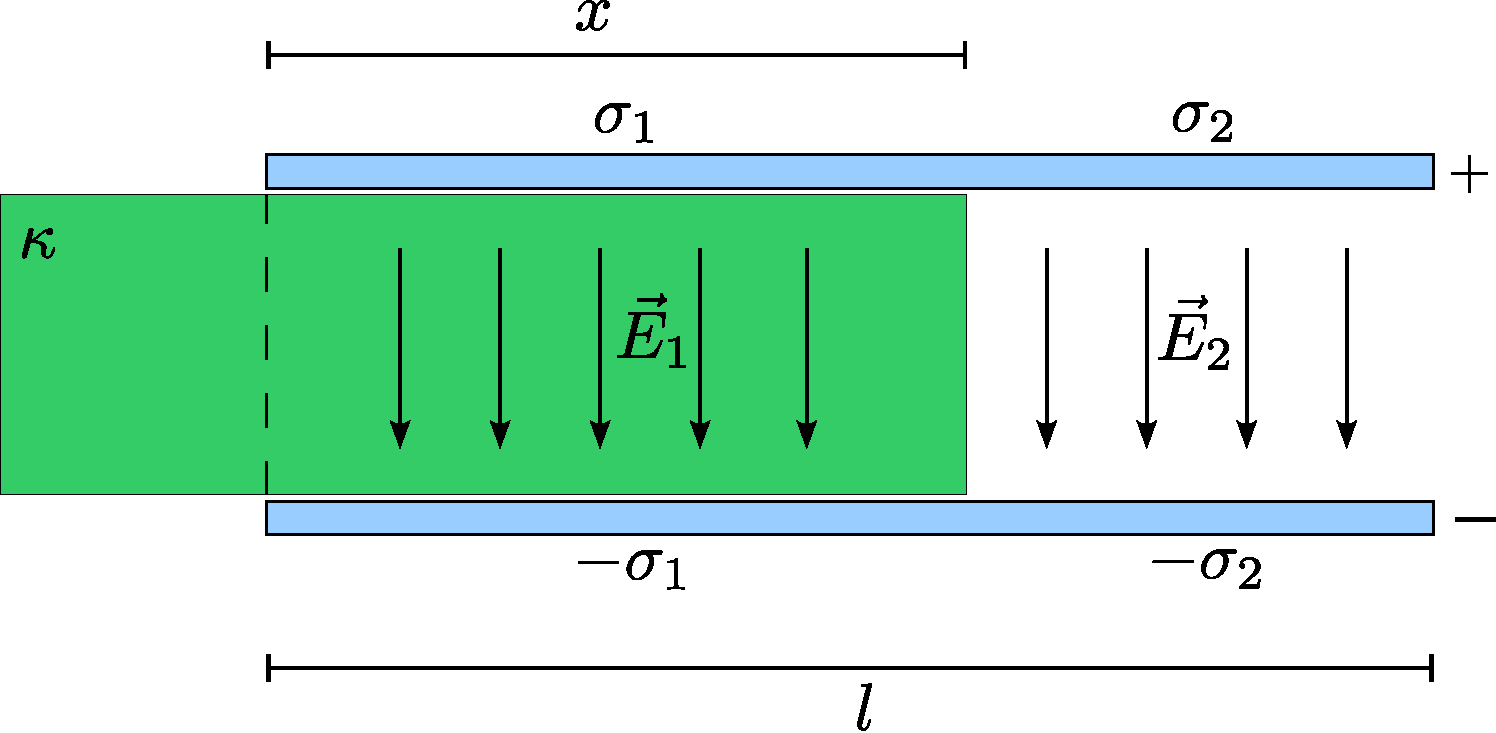
\psfig{file=fig/fig-condensador-semi-lleno-01.pdf , height=4cm ,
angle=0}}
\caption{Condensador parcialmente lleno con diel'ectrico.}
\label{fig:fccd}
\end{figure}
Consideremos el caso en que el sistema est'a cargado, con cargas $+Q$ y $-Q$
respectivamente, y aislado. Debemos determinar los campos en la regi'on con
diel'ectrico (regi'on 1) y sin 'el (regi'on 2). Despreciando efectos de borde,
podemos aproximar que todos los campos son verticales, con sus sentidos hacia
abajo en la figura. Ya que la componente tangencial del campo el'ectrico es
continua en una interfase entre dos diel'ectricos, encontramos que el campo
el'ectrico $\vec{E}$ es igual en todo punto entre las placas del condensador,
es decir,
\begin{equation}
 E_1=E_2.
\end{equation}
Usando (\ref{GaussD}) encontramos directamente que
\begin{equation}
 D_1=\varepsilon_0\kappa E=\sigma_1, \qquad D_2=\varepsilon_0 E=\sigma_2,
\end{equation}
donde $\sigma_1$ y $\sigma_2$ son las densidades de carga en las placas en la
regi'on correspondiente. La carga total en cada placa es entonces dada por
\begin{eqnarray}
 Q&=&\sigma_1A_1+\sigma_2A_2 \\
&=& \varepsilon_0\kappa E w x+\varepsilon_0E w (l-x) \\
&=& \varepsilon_0Ew\left(\kappa x+l-x\right), \label{Qej}
\end{eqnarray}
donde $w$ es la longitud de la otra arista del rect'angulo que define cada placa (es decir, en la direcci'on perpendicular a la figura \ref{fig:fccd}).

La energ'ia electrost'atica del sistema puede ser calculada evaluando
(\ref{UED}):
\begin{eqnarray}
 U&=&\frac{1}{2}\int\vec{D}\cdot\vec{E}\,dV \\
&=&\frac{1}{2}\left(D_1EV_1+D_2EV_2\right) \\
&=&\frac{1}{2}\left[\varepsilon_0\kappa
xwd+\varepsilon_0(l-x)wd\right]E^2 \\
&=&\frac{1}{2}\varepsilon_0\left(\kappa x+l-x\right)wdE^2 .
\end{eqnarray}
Usando (\ref{Qej}), podemos finalmente expresar la energ'ia electrost'atica
del sistema como
\begin{equation}
U(x)=\frac{Q^2d}{2\varepsilon_0 w}\frac{1}{(\kappa x+l-x)}.
\end{equation}
Ya que el sistema est'a aislado y $Q$ es constante, la fuerza sobre el
diel'ectrico puede ser calculada a partir de (\ref{FQ}). As'i obtenemos
\begin{equation}
 F(x)=\frac{Q^2d}{2\varepsilon_0 w}\frac{(\kappa-1)}{(\kappa x+l-x)^2},
\end{equation}
que es una fuerza que \textit{atrae al diel'ectrico hacia el interior de las
placas}.

\subsubsection{Ejemplo: Electr'ometro}
\newpage
\chapter{Magnetoest'atica}


\section{Corriente y densidad de corriente}

Cuando existen cargas en movimiento, se define la \textit{corriente el'ectrica} $I$ como
la cantidad de \textit{carga neta} que pasa por unidad de tiempo a trav'es de una superficie $S$ \textit{en una direcci'on determinada}, 
\begin{equation}\marginnote{Corriente el'ectrica}
I(t) :=\lim_{\Delta t\to 0}\frac{\Delta Q}{\Delta t}=\frac{dQ}{dt},
\end{equation}
de modo que la carga neta que atraviesa entre los tiempos $t_1$ y $t_2$ una superficie por donde circula una corriente $I(t)$ es
\begin{equation}
Q=\int_{t_1}^{t_2}I(t)\,dt.
\end{equation}
La unidad S.I. para la corriente es el \textbf{Amp\`ere}: $1A:=1C/1s$.

\subsection{Densidad de Corriente}

Consideremos una superficie sobre la cual inciden cargas con densidad $\rho$,
movi'endose con velocidad $\vec{v}$, cruzando un elemento de superficie (orientado) $d\vec{S}$.
\begin{figure}[!h]
\centerline{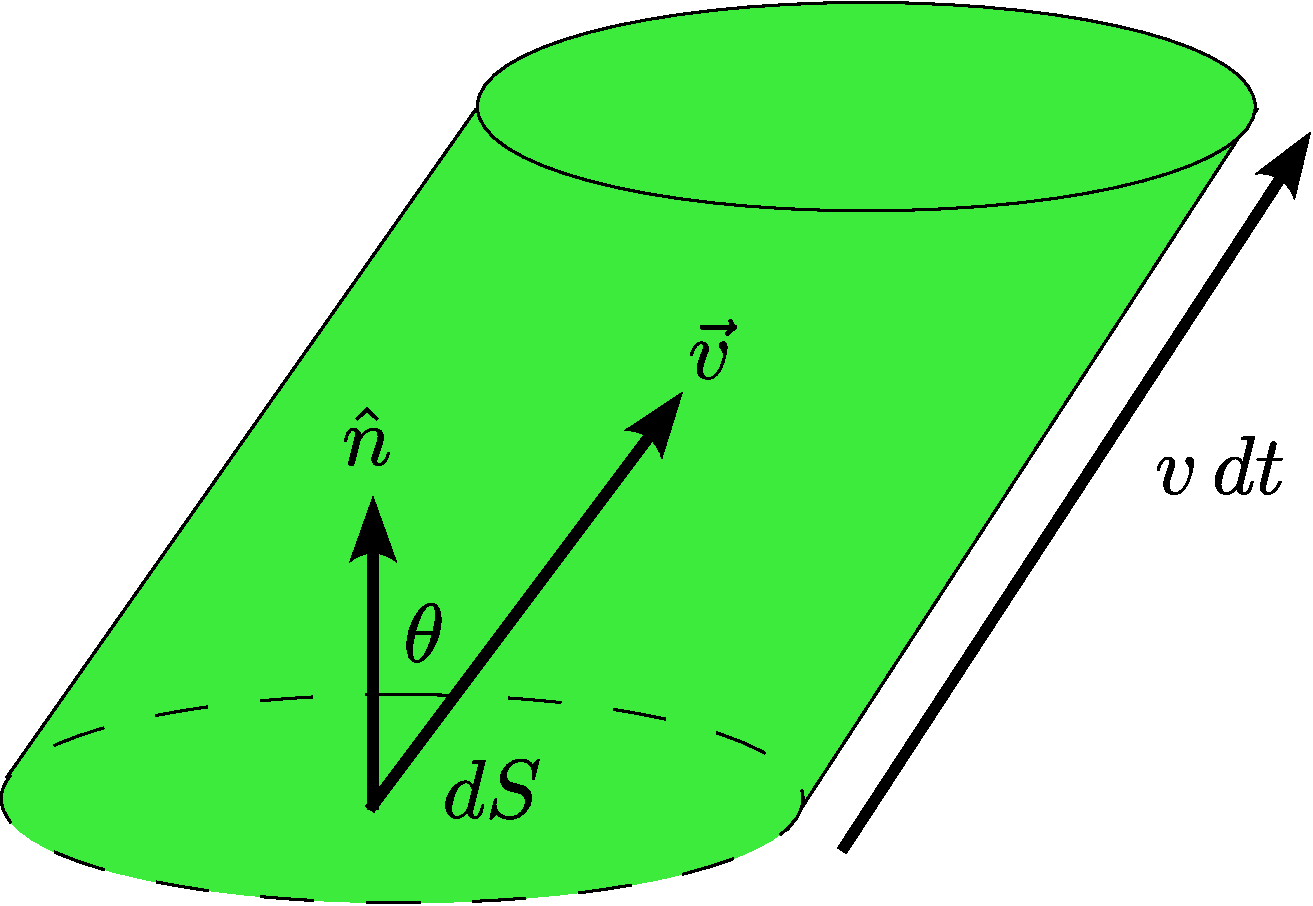
\psfig{file=fig/fig-flujo-cargas-01.pdf,height=4cm,angle=0}}
\caption{Carga con densidad $\rho$ flujendo con velocidad $\vec{v}$ a trav'es
de un elemento de superficie $d\vec{S}$.}
\label{MD1}
\end{figure}
La carga neta que atraviesa el 'area $dS$ en un intervalo de tiempo $dt$ es la que
est'a contenida en un cilindro oblicuo de base $dS$ y de largo $v\,dt$. Ver
figura \ref{MD1}.

Esto permite escribir:
\begin{equation}
dQ=\rho\, dV=\rho\, dS\,(v\,dt)\cos\theta=\rho\,\vec{v}\cdot d\vec{S}\,dt.
\end{equation}
Definimos la \textbf{densidad de corriente}
\begin{equation}\marginnote{Densidad de Corriente}
\boxed{\vec{J}(x):=\rho(x)\vec{v}(x),}
\end{equation}
de modo que
\begin{equation}
 dQ=\vec{J}\cdot d\vec{S}\,dt .
\end{equation}
En otras palabras, la densidad de corriente es la carga por unidad de tiempo y
por unidad de superficie que atraviesa un elemento de 'area normal dado.
Como consecuencia, la corriente, es decir, la carga por unidad de tiempo,
que atraviesa una superficie $S$ es dada por
\begin{equation}
I=\int_{S}\vec{J}\cdot d\vec{S}.
\end{equation}
Es importante notar que si $\rho>0$, entonces $\vec{J}$ y $\vec{v}$ tienen igual
sentido, mientras que si $\rho<0$, entonces $\vec{J}$ y $\vec{v}$ tienen
sentidos opuestos.

\section{Conservaci'on de la carga el'ectrica}

La ley (experimental) de conservaci'on (local) de la carga el'ectrica puede ser escrita
en general, como
\begin{equation}
\frac{d{\ }}{dt}\int_V \rho\,dV=-\int_{\partial V}\vec{J}\cdot d\vec{S},
\end{equation}
que expresa el hecho que todo cambio en la carga neta contenida en un volumen $V$ dado (pero arbitrario) es debido al flujo neto de carga por la superficie ${\partial V}$ que lo encierra. Usando el teorema de Gauss, podemos transformar la integral de superficie a una integral de volumen, obteniendo
\begin{equation}
\int_V\left(\frac{\partial\rho}{\partial t}+\vec{\nabla}\cdot\vec{J}\right)\,dV
 =0.
\end{equation}
Como esta relaci'on debe ser v'alida para todo volumen $V$, es decir, de tama\~no y forma arbitraria, es necesario que
\begin{equation}\marginnote{Conservaci'on local carga}
\boxed{\frac{\partial\rho}{\partial t}
+\vec{\nabla}\cdot\vec{J}=0.}\label{eccont}
\end{equation}
Esta relaci'on es conocida como la \textit{ecuaci'on de continuidad}.

\subsection{Corrientes Estacionarias}

Un caso de particular inter'es es aquel en que las corrientes son
\textit{estacionarias}, es decir, en las que tanto $\rho$ como $\vec{J}$ \textit{no dependen del tiempo}. Bajo estas condiciones, la ecuaci'on de continuidad requiere que la
divergencia de la densidad de corriente sea nula:
\begin{equation}\marginnote{Caso estacionario}
 \vec{\nabla}\cdot\vec{J}=0. \label{divJ0}
\end{equation}


% \subsection{Modelo de Conductividad}
%
% Suponemos que los electrones se mueven en la red at'omica. La ecuaci'on
% de movimiento es
% \begin{equation}
% mn\frac{du_i}{dt} -nqE_i=F_i%
% \label{magstatica-mov}%
% \end{equation}
% donde $T$ es la temperatura del gas de electrones, y $F_i=-mn\nu u_i$ es
% la fuerza debido a las colisiones. Recordando que $\rho=nq$ y que
% $j_i=nqu_i$ tenemos que en la ecuaci'on (\ref{eccont} )
% resulta%
% \begin{equation}
% \frac{\partial\rho}{\partial t}+\partial_i\left(  \rho u_i\right)  =0
% \end{equation}
% de la ecuaci'on (\ref{magstatica-mov}) y suponiendo que el gradiente de
% temperatura es despreciable, tenemos%
% \begin{align*}
% mn\frac{du_i}{dt}-nqE_i  & =-mn\nu u_i\\
% n\frac{d\left(  u_i\right)  }{dt}  & =\frac{nq}{m}E_i-\nu u_i%
% \qquad\qquad/\cdot q\\
% \frac{d\left(  nqu_i\right)  }{dt}  & =\frac{nq^2}{m}E_i-\nu nqu_i\\
% \frac{dj_i}{dt}+\nu j_i  & =\frac{nq^2}{m}E_i%
% \end{align*}
% Si $\vec{J}$ es constante en el tiempo%
% \begin{equation}
% j_i=\frac{nq^2}{m\nu}E_i=\sigma E_i%
% \end{equation}
% llamando a $\sigma$ conductividad el'ectrica. Notar que la conductividad es
% inverso a la resistencia el'ectrica, es decir, $\sigma=1/R~~\left[
% 1/\Omega\right]  $

% \subsubsection{Aplicaci'on: Velocidad de distribuci'on de la carga}
%
% Velocidad con que se distribuye la carga el'ectrica en un conductor con
% conductividad $\sigma$. Veamos que,%
% \begin{equation}
% j_i=\sigma E_i%
% \end{equation}
% luego en la euaci'on de continuidad (\ref{eccont} ) tenemos%
% \begin{align*}
% \frac{\partial\rho}{\partial t}+\vec{\nabla}\cdot\vec{J}  & =0\\
% \frac{\partial\rho}{\partial t}+\sigma\partial_iE_i  & =0\\
% \frac{\partial\rho}{\partial t}+\frac{\sigma}{\varepsilon_0}\rho & =0
% \end{align*}
% Esta ecuaci'on diferencial tiene como soluci'on%
% \begin{equation}
% \rho(t)=\rho_0~e^{-t/t_0}%
% \end{equation}
% donde $t_0=\varepsilon_0/\sigma$. Para valores experimentales tenemos que
% $\varepsilon_0=8.8512\times10^{-12}~\left[  c^2/Nm^2\right]  $ y para el
% cobre se tiene que $\sigma=59.88~\left[  1/\Omega\right]  $ luego conociendo
% la densidad del cobre podemos saber como varia la densidad de carga en el
% tiempo para un volumen dado.

\section{Campo magn'etico y fuerza magn'etica}
Se ha encontrado \textit{experimentalmente} que la fuerza que act'ua sobre una peque\~na carga $q$, movi'endose con velocidad $\vec{v}$ en un campo magn'etico dado es proporcional a $q$, a la rapidez $v$, y que tiene direcci'on perpendicular a $\vec{v}$. Esto permite \textit{definir}  la \textit{intensidad de campo magn'etico} $\vec{B}$ como un (pseudo-)vector tal que (en el sistema internacional de unidades)
\begin{equation}
 \vec{F}_{\rm m}=q\,\vec{v}\times\vec{B}.
\end{equation}
Por lo tanto, la fuerza total que act'ua sobre una carga $q$ en un punto del espacio con campo el'ectrico $\vec{E}$ y magn'etico $\vec{B}$ es dada por la \textit{fuerza de Lorentz}\footnote{En honor a Hendrik Antoon Lorentz (1853-1928): f'isico y matem'atico holand'es. Ganador del Premio Nobel de F'isica en 1902. Ver \url{http://es.wikipedia.org/wiki/Hendrik_Lorentz}.}
\begin{equation}\marginnote{Fuerza de Lorentz}
\boxed{ \vec{F}=q\left(\vec{E}+\vec{v}\times\vec{B}\right).}
\end{equation}
La unidad de medida de la intensidad de campo magn'etico $\vec{B}$ es entonces  $[B]=Ns/Cm=Vs/m^2$ , que se define como un \textit{Tesla}: $1T:=Vs/m^2$. Alternativamente se define un
\textit{Gauss} como $1G:=10^{-4}T$. \footnote{Por ejemplo, la magnitud campo
magn'etico interestelar oscila entre $0,1$ and $10$ $nT$, el campo magn'etico
de la Tierra es de orden $\approx 0,5 G$, mientras que un im'an
de Neodimio (Nd${}_2$Fe${}_{14}$B) produce un campo del orden de $1.25\, T$.
Un magneto de un sistema de resonancia magn'etica produce campos entre $1,5\,T$
y $3\,T$. Los campos magn'eticos m'as intensos producidos en un laboratorio son
del orden de $100\,T$ \cite{MagLab2012,HZDR2011}. El campo magn'etico en una estrella de neutrones puede oscilar entre 1 y 100 MT.}

Como consecuencia directa del hecho que la fuerza magn'etica es perpendicular a
la velocidad de las cargas, \textit{el campo magn'etico no realiza trabajo} sobre ellas.
Esto tiene como consecuencia que el campo magn'etico s'olo puede cambiar la
direcci'on de la velocidad de una carga y no su m'odulo (energ'ia cin'etica).

Si las cargas est'an distribuidas continuamente, entonces la fuerza magn'etica total sobre una regi'on $V$ con densidad $\rho$ y velocidad $\vec{v}$ ser'a
\begin{equation}\marginnote{Fuerza magn'etica}
 \vec{F}_{\rm m}=\int_V
\rho\vec{v}\times\vec{B}\,dV=\int_V\vec{J}\times\vec{B}\,dV. \label{fm1}
\end{equation}
Podemos describir esta situaci'on usando la \textbf{densidad de fuerza
magn'etica} $\vec{f}_{\rm m}$, definida como la fuerza por unidad de volumen,
dada por
\begin{equation}
 \vec{f}_{\rm m}:=\vec{J}\times\vec{B},
\end{equation}
de modo que
 \begin{equation}
\vec{F}_{\rm m}=\int_V\vec{f}_{\rm m}\,dV. \label{dfm}
\end{equation}


% \subsection{Trayectorias en un campo el'ectromagn'etico}
% Usando () y la segunda ley de Newton, tenemos
% \begin{equation}
% m\frac{dv_i}{dt}=qE_i+q\varepsilon_{ijk}v_jB_k
% \end{equation}
% Multiplicando esta ecuaci'on con $v_i$, obtenemos
% \begin{equation}
%  \frac{d\ }{dt}(\frac{m}{2}v^2)=qv_iE_i
% \end{equation}
% \begin{equation}
%  \frac{dK}{dt}=qv_iE_i
% \end{equation}
% S'olo el campo el'ectrico realiza trabajo sobre la carga, modificando su
% energ'ia ci'n'etica.
% \begin{equation}
%  dK=qv_iE_idt=qE_idx_i=-q\partial_i\phi dx_i=-qd\phi
% \end{equation}
% \begin{equation}
%  d(K+q\phi)=0
% \end{equation}
% \begin{equation}
%  \frac{1}{2}mv^2+q\phi={\rm cte}
% \end{equation}
% a lo largo de la trayectoria.


\section{Ley de Biot-Savart}
Biot\footnote{Jean Baptiste Biot: F'isico, Astr'onomo y Matem'atico franc'es (1774-1862). Ver \url{http://es.wikipedia.org/wiki/Jean_Baptiste_Biot}.} y Savart\footnote{F'elix Savart: F'isico, M'edico y Profesor franc'es (1791-1841). Ver \url{http://es.wikipedia.org/wiki/F\%C3\%A9lix_Savart}.} encontraron ($\sim$\,1820) que el campo magn'etico $d\vec{B}$ que un peque\~no segmento $dx'$ orientado en la direcci'on de flujo de la corriente $I$ y ubicado en la posici'on $\vec{x}'$ produce en un punto de posici'on $\vec{x}$ es proporcional a la intensidad de corriente, al largo del
peque\~no segmento, e inversamente proporcional al cuadrado de la distancia
entre el segmento y el punto de observaci'on, es decir,
\begin{equation}
 \left\vert d\vec{B}\right\vert \propto
\left(I,dx',\frac{1}{\left|\vec{x}-\vec{x}'\right|^2}\right),
\end{equation}
y que la direcci'on del campo producido es perpendicular a $d\vec{x}'$ y al
vector que une el segmento con el punto de observaci'on,
\begin{equation}
d\vec{B}  \perp\left(  d\vec{x}', \vec{x}-\vec{x}' \right) ,
\end{equation}
y que, finalmente, el sentido del campo magn'etico es dado por la regla de la mano derecha a partir de los vectores $d\vec{x}'$ y $\vec{x}-\vec{x}'$. Ver figura \ref{fBS1}. 
\begin{figure}[!h]
\centerline{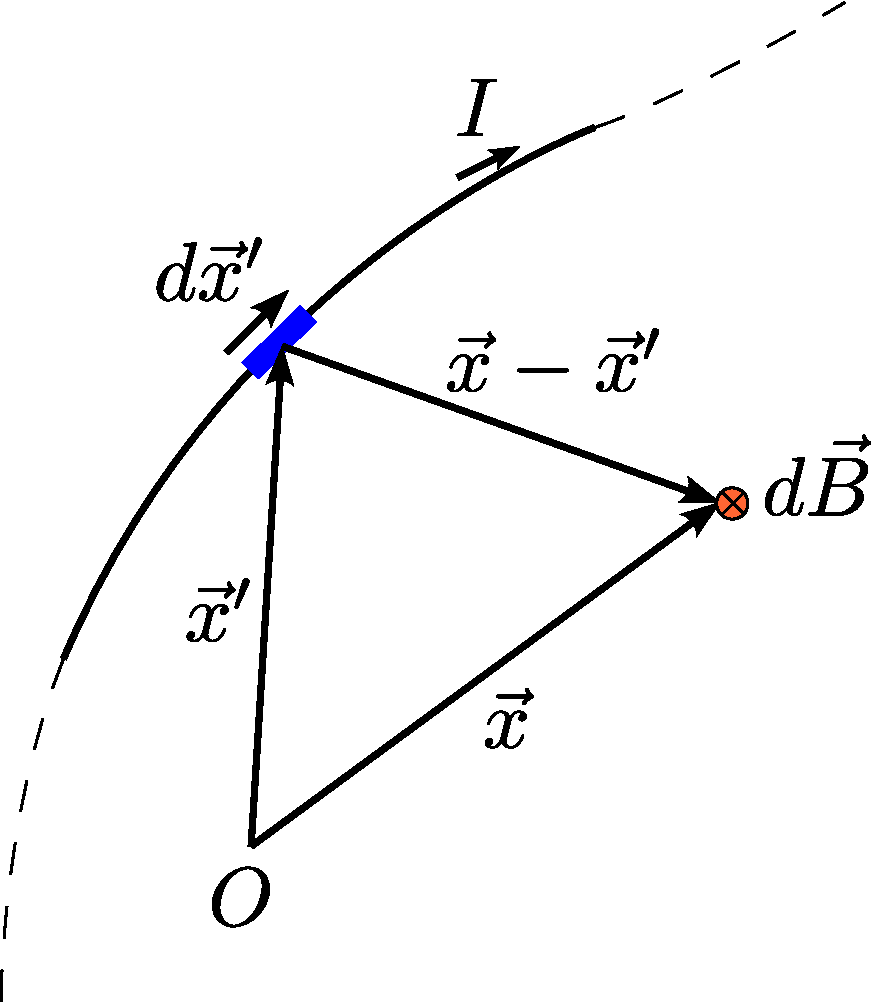
\psfig{file=fig/fig-Biot-Savart-01.pdf,height=6cm,angle=0}}
\label{Esquema para la ley de Biot-Savart.}
\label{fBS1}
\caption{Ley de Biot-Savart.}
\end{figure}
En resumen,
\begin{equation}
dB_i=kI\varepsilon_{ijk}dx'_j\frac{\left(x_k-x'_k\right)}{\left\vert
\vec{x}-\vec{x}'\right\vert^3},
\end{equation}
donde $k$ es una constante, que depende del sistema de unidades usado y que,
en el Sistema Internacional, \textit{se define} como
\begin{equation}
k=\frac{\mu_0}{4\pi}=10^{-7}~\left[  \frac{V\,s}{A\,m}\right],
\end{equation}
y donde $\mu_0$ es llamada la constante de \textbf{permeabilidad magn'etica del vac'io}.

Con esto, escribimos la \textbf{ley de Biot-Savart} como
\begin{equation}
dB_i=\frac{\mu_0}{4\pi}I\,\varepsilon_{ijk}dx'_j\frac{\left(x_k-x'_k\right)}
{\left\vert \vec{x}-\vec{x}'\right\vert ^3}.
\end{equation}
Usando el \textbf{principio de superposici'on} obtenemos una expresi'on para el campo producido por un cable de longitud finita, pero muy delgado:
\begin{equation}
\boxed{B_i(x)=\frac{\mu_0}{4\pi}\int_{\cal C}\varepsilon_{ijk}Idx'_j
\frac{\left(x_k-x'_k\right)}{\left\vert\vec{x}-\vec{x}'\right\vert^3}.}
\label{BS1}
\end{equation}

Podemos generalizar este resultado al caso de una distribuci'on volum'etrica de corriente, descrita por su densidad de corriente. Para esto, consideramos un peque\~no ``tubo de corriente"\, de secci'on transversal $dS$ que sigue las l'ineas de flujo, es decir, tal que el vector normal a la superficie transversal, $\hat{n}$, es paralalo a $\vec{J}$. Entonces, $\vec{J}=J\hat{n}$, $d\vec{x}=d\ell\,\hat{n}$, y adem'as $dV=d\ell\, dS$ (ver figura \ref{fig:tc}), de modo que podemos escribir
\begin{equation}
I\, d\vec{x}=(J dS)(\hat{n}d\ell)=(J\hat{n})(d\ell dS)=\vec{J}\,dV.
\end{equation}
\begin{figure}[!h]
\centerline{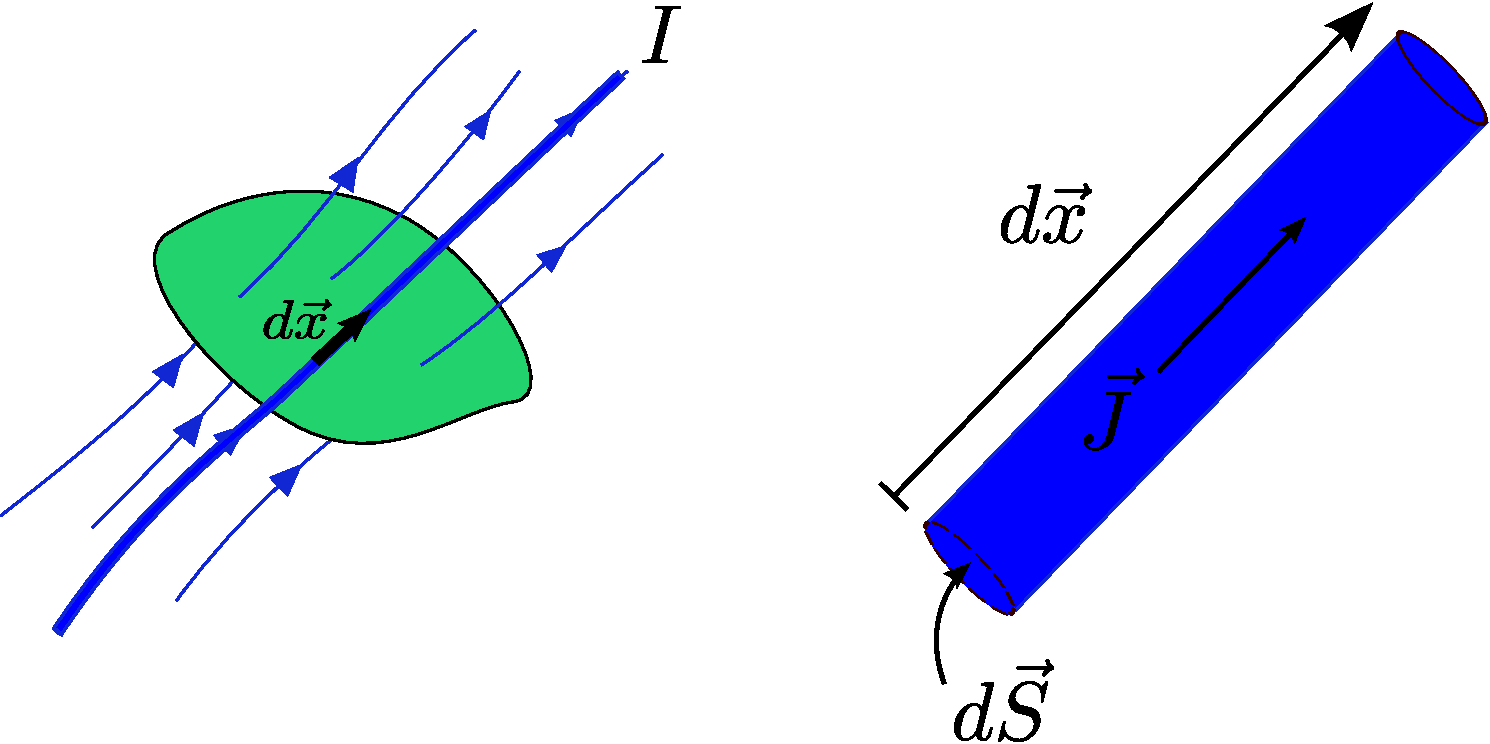
\psfig{file=fig/fig-tubo-de-corriente.pdf,height=4cm,angle=0}}
\caption{Una distribuci'on volum'etrica y los ``tubos de corriente'' asociados.}
\label{fig:tc}
\end{figure}
Con esto podemos encontrar la forma general que usaremos para la ley de Biot-Savart:
\begin{equation}\marginnote{Ley de Biot-Savart}
 \boxed{B_i(x)=\frac{\mu_0}{4\pi}\int_V\varepsilon_{ijk}\,J_j(x')
\frac{\left(x_k-x'_k\right)}{\left\vert\vec{x}-\vec{x}'\right\vert^3}dV'. }
\label{BS2}
\end{equation}
Tambi'en podemos considerar una \textit{distribuci'on superficial de corriente}, es decir una situaci'on donde puede \textit{aproximarse} que la corriente est'a confinada sobre una superficie (de ancho nulo). Para describir esta distribuci'on usamos la \textbf{densidad superficial de corriente}, que denotaremos como $\vec{j}$. Esta densidad superficial es definida tal que
\begin{equation}
\vec{J}\,dV=\vec{j}\,dS,
\end{equation}
donde $dS$ denota el elemento de superficie \textit{sobre} (y no \textit{a trav'es} de) la que fluye la corriente. El campo magn'etico generado por este tipo de distribuciones adopta entonces la forma siguiente:
\begin{equation}
 \boxed{B_i(x)=\frac{\mu_0}{4\pi}\int_S\varepsilon_{ijk}\,j_j(x')
\frac{\left(x_k-x'_k\right)}{\left\vert\vec{x}-\vec{x}'\right\vert^3}dS'. }
\label{BSsup}
\end{equation}
Tal como en el estudio del campo electrost'atico, trabajaremos con la expresi'on volum'etrica \eqref{BS1}, que es m'as general. Si se requiere adaptar las expresiones al caso de corrientes superficiales o lineales pueden entonces usarse las siguientes reglas de conversi'on:
\begin{equation}\label{IdxJdV}
\vec{J}\,dV=\vec{j}\,dS=I\,d\vec{x}.
\end{equation}
Note adem'as que si la corriente es siempre producida por una distribuci'on de cargas movi'endose con velocidad $\vec{v}$ entonces 
\begin{equation}
\vec{J}=\rho\vec{v}, \qquad \vec{j}=\sigma\vec{v}, \qquad I=\lambda v,
\end{equation}
donde $\rho$, $\sigma$ y $\lambda$ son las densidad de carga por unidad de volumen, superficie y longitud, en el caso de distribuciones de corriente volum'etrica, superficial y lineal, respectivamente.

\section{Potencial vectorial}
Consideramos ahora la identidad
\begin{equation}
\frac{x_k-x'_k}{\left\vert
\vec{x}-\vec{x}'\right\vert^3}\equiv -\partial_k\left(
\frac{1}{\left\vert\vec{x}-\vec{x}'\right\vert }\right).
\end{equation}
Reemplaz'andola en (\ref{BS2}) encontramos
\begin{eqnarray}
 B_i(x)&=&-\frac{\mu_0}{4\pi}\int_V\varepsilon_{ijk}\,J_j(x')
\partial_k\left(\frac{1}{\left\vert\vec{x}-\vec{x}'\right\vert }\right)dV'
\label{BS3} \\
&=&-\varepsilon_{ijk}\,\partial_k\left(\frac{\mu_0}{4\pi}\int_VJ_j(x')\frac{1}{
\left\vert\vec{x} -\vec{x}'\right\vert }dV'\right)\\
&=&\varepsilon_{ijk}\,\partial_j\left(\frac{\mu_0}{4\pi}\int_VJ_k(x')\frac{1}{
\left\vert\vec{x} -\vec{x}'\right\vert }dV'\right).
\end{eqnarray}
Por lo tanto, siempre es posible escribir el campo magnetost'atico como el rotor de un campo vectorial,
\begin{equation}\marginnote{Potencial Vectorial}
\boxed{B_i(x)=\varepsilon_{ijk}\,\partial_jA_k(x),}\label{rot-A}
\end{equation}
donde hemos introducido el \textbf{potencial vectorial},
\begin{equation}\marginnote{Pot. Vectorial particular}
\boxed{A_k(x):=\frac{\mu_0}{4\pi}\int_V\frac{J_k(x')}{\left\vert\vec{x}-\vec{x}
'\right\vert }\,dV'.}
\label{defA}
\end{equation}
An'alogamente al caso electrost'atico, el \textit{potencial vectorial no es \'{u}nico}. En el caso magn'etico, sin embargo, la situaci'on es algo menos trivial ya que es posible considerar un nuevo potencial vectorial
\begin{equation}
A'_i:=A_i+\partial_i\Psi(x), \label{gauge01}
\end{equation}
donde $\Psi(x)$ es una \textit{funci'on arbitraria}, y el campo magn'etico
permanecer'a inalterado, ya que $B'_i(x)=\varepsilon_{ijk}\,\partial_jA'_k(x)=B_i(x)$. La transformaci'on (\ref{gauge01}) es llamada una \textbf{transformaci'on de gauge}
del potencial vectorial. Como consecuencia, el potencial vectorial $\vec{A}(x)$
\textit{no es una cantidad medible}, sino m'as bien un campo auxiliar (muy)
'util en muchos c'alculos. En general, a menos que se explicite lo contrario,
cuando hablemos del potencial vectorial magn'etico nos referiremos la elecci'on particular 
dada por (\ref{defA}).


\section{Divergencia del Campo Magn'etico}

Como consecuencia directa de (\ref{rot-A}), vemos que \textit{el campo magnetost'atico
es siempre libre de divergencia}:
\begin{equation}
 \boxed{\vec{\nabla}\cdot\vec{B}=0.} \label{divB}
\end{equation}
Equivalentemente,
\begin{equation}
 \oint_S\vec{B}\cdot d\vec{S}=0,
\end{equation}
es decir, que el \textbf{flujo magn'etico} a trav'es de cualquier superficie cerrada es nulo.

Recordemos que el flujo magn'etico a trav'es de una superficie $S$ es definido
como
\begin{equation}
 \Phi_S:= \int_S\vec{B}\cdot d\vec{S}.
\end{equation}
Usando (\ref{rot-A}) y el teorema de Stokes encontramos que
\begin{equation}\label{PAdx}
 \Phi_S=\oint_{\partial S}\vec{A}\cdot d\vec{x},
\end{equation}
es decir, que el flujo magn'etico a trav'es de una superficie s'olo depende del
valor del potencial vectorial sobre la curva (orientada) $\partial S$ que delimita $S$.
Puede verificarse adem'as que, si bien la expresi'on anterior involucra el
potencial vectorial, \textit{el valor del flujo $\Phi_S$ es independiente de la
elecci'on particular de $\vec{A}$} dentro de la familia de potenciales
vectoriales asociados a un campo $\vec B$ dado. En otras palabras el flujo es
\textbf{invariante} bajo transformaciones de gauge. Note adem'as que, debido a la
relaci'on entre $\Phi_S$ y $\vec{B}$ este 'ultimo vector es tambi'en llamado
\textbf{densidad de flujo magn'etico}. En el sistema internacional de unidades, se define el \textit{Weber}\footnote{En honor a Wilhelm Weber, f'isico alem'an (1804-1891). Ver \url{http://es.wikipedia.org/wiki/Wilhelm_Weber}.} como unidad de flujo magn'etico: $1Wb=1T\cdot 1m^2=1V\cdot 1s$.

\section{Ley de Amp\`ere}

Queremos calcular el rotor de la intensidad de campo magn'etico, es decir, $\varepsilon_{ijk}\partial_jB_k$. Usando (\ref{rot-A})
podemos escribir:
\begin{eqnarray}
 \varepsilon_{ijk}\partial_jB_k&=&\varepsilon_{ijk}\varepsilon_{
klm}\partial_j\partial_lA_m \\
&=&\partial_i(\partial_jA_j) -\partial_j\partial_jA_i. \label{rotB1}
\end{eqnarray}
Para evaluar esta expresi'on usaremos el potencial definido por (\ref{defA})
(el resultado final es independiente de la elecci'on de $\vec{A}$ ya que s'olo
depende de $\vec{B}$). Calculemos primero la divergencia del potencial
vectorial:
\begin{eqnarray}
\partial_iA_i&=&\frac{\mu_0}{4\pi}\int_VJ_i(x')\partial_i\frac{1}{\left\vert\vec
{x} -\vec{x}'\right\vert }\,dV' \\
&=& -\frac{\mu_0}{4\pi}\int_VJ_i(x')\partial'_i\frac{1}{\left\vert\vec{
x } -\vec{x}'\right\vert }\,dV' \\
&=&-\frac{\mu_0}{4\pi}\int_V\left[\partial'_i\left(\frac{J_i(x')}{
\left\vert\vec{x}-\vec{x}'\right\vert}\right)-\frac{
\left(\partial'_iJ_i(x')\right) } { \left\vert\vec{x} -\vec{x}'\right\vert
}\right]\,dV' \\
&=&-\frac{\mu_0}{4\pi}\oint_{\partial V}\frac{J_i(x')}{
\left\vert\vec{x}-\vec{x}'\right\vert}dS'_i+\frac{\mu_0}{4\pi}\int_V\frac{
\left(\partial'_iJ_i(x')\right) } {\left\vert\vec{x}
-\vec{x}'\right\vert}\,dV'  \label{divA} \\
&=&0. \label{divA0}
\end{eqnarray}
El primer t'ermino del lado derecho de (\ref{divA}) se anula cuando cuando $V$
se extiende a todo el espacio, puesto que suponemos que la densidad de corriente
se anula suficientemente r'apido en el infinito (m'as r'apido que $1/r$). Adem'as, el segundo t'ermino es nulo \textit{para corrientes estacionarias}, ver (\ref{divJ0}). Por lo tanto, hemos probado que el potencial (\ref{defA}) tiene divergencia nula en el caso de corrientes
estacionarias confinadas a regiones compactas del espacio.

Debemos ahora calcular el laplaciano (de cada una de las componentes) de
$\vec{A}$. De la definici'on (\ref{defA}) encontramos que
\begin{eqnarray}
 \nabla^2A_i&=&\frac{\mu_0}{4\pi}\int_VJ_i(x')\nabla^2\frac{1}{\left\vert\vec{
x } -\vec{x}'\right\vert }\,dV'\\
&=&\frac{\mu_0}{4\pi}\int_VJ_i(x')\left(-4\pi\delta^{(3)}(\vec{x}-\vec{x}
')\right)\,dV' \\
&=&-\mu_0J_i(x). \label{lapAj}
\end{eqnarray}
Reemplazando (\ref{divA0}) y (\ref{lapAj}) en (\ref{rotB1}) encontramos la
\textbf{ley de Amp\`ere}\footnote{\href{http://es.wikipedia.org/wiki/Andr\%C3\%A9-Marie_Amp\%C3\%A8re}{Andr'e-Marie Amp\`ere} (1775-1836): matem'atico y f'isico franc'es.}:
\begin{equation}
\boxed{\varepsilon_{ijk}\partial_jB_k=\mu_0J_i,}
\end{equation}
o, en notaci'on vectorial,
\begin{equation}\marginnote{Ley Amp\`ere (diferencial)}
 \boxed{\vec\nabla\times\vec{B}=\mu_0\vec{J}.}\label{ley-Ampere}
\end{equation}
La versi'on integral de la ley de Amp\`ere (obtenida integrando
(\ref{ley-Ampere}) en una superficie $S$ con borde $\partial S$, y usando el
teorema de Stokes) es
\begin{equation}\marginnote{Ley Amp\`ere (integral)}
 \boxed{\oint_{\partial S}\vec{B}\cdot d\vec{x}=\mu_0 I_S,}
\end{equation}
donde $I_S=\int_S\vec{J}\cdot d\vec{S}$ es la corriente neta que fluye por $S$.

\subsection{Ejemplo: Campo magn'etico producido por una l'inea infinita de
corriente}
\begin{figure}[!h]
\centerline{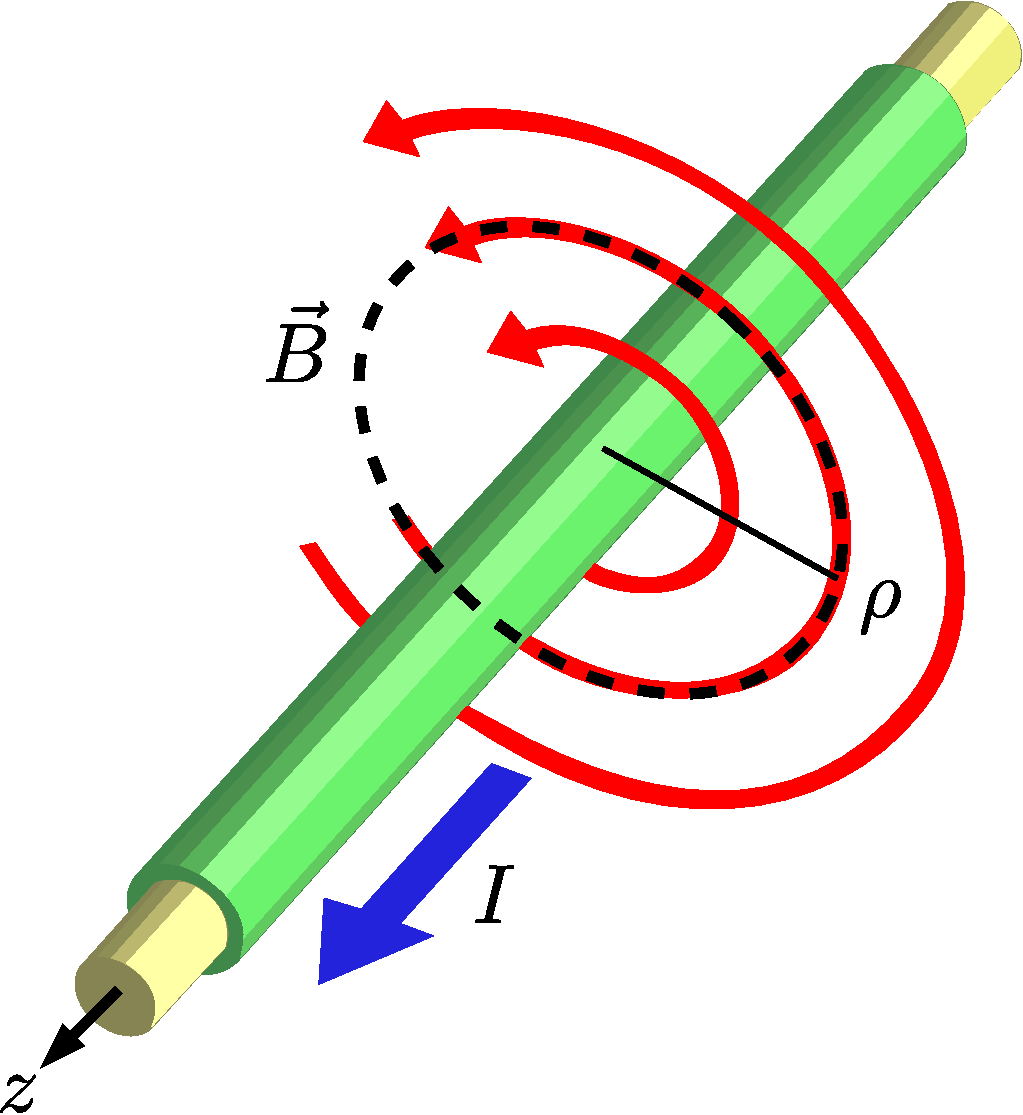
\psfig{file=fig/fig-B-conductor-recto-01.pdf,height=5cm,angle=0}}
\caption{Campo magn'etico producido por un conductor recto. Figura original  \href{http://en.wikipedia.org/wiki/File:Electromagnetism.svg}{aqu\'i}.}
\label{cmcr}
\end{figure}
Aplicando la ley de Amp\`ere a la circunsferencia de radio $\rho$ indicada en la figura
(\ref{cmcr}) encontramos que
\begin{equation}
 \oint_{\cal C}\vec{B}\cdot d\vec{x}=(2\pi \rho)B=\mu_0 I,
\end{equation}
de modo que
\begin{equation}
\vec{B}(\rho)=\frac{\mu_0I}{2\pi}\frac{\hat{\varphi}}{\rho}.
\end{equation}
Un potencial vectorial posible para describir este campo es
\begin{equation}
 \vec{A}_1(\rho)=-\frac{\mu_0I}{2\pi}\ln\frac{\rho}{\rho_0} \hat{z}.
\end{equation}
Sin embargo, otro potencial posible es
\begin{equation}
 \vec{A}_2(z)=\frac{\mu_0I}{2\pi}\frac{z}{\rho} \hat{\rho}.
\end{equation}


\section{Potencial escalar magn'etico}\label{secpem}
En regiones en las que no existen corrientes, $\vec{J}=\vec{0}$, el
rotor del campo magn'etico es nulo, $\vec{\nabla}\times\vec{B}=\vec{0}$. En
este caso es \textit{posible escribir $\vec{B}$ como el gradiente de un campo escalar},
\begin{equation}\marginnote{Potencial Escalar Magn'etico}
 \vec{B}=-\mu_0\vec\nabla\phi^*, \label{Bgradphi}
\end{equation}
donde $\phi^*$ es llamado \textbf{potencial escalar magn'etico}. Ya que adem'as
el campo magn'etico es (siempre) libre de divergencias, tenemos que
\begin{equation}
 \boxed{\nabla^2\phi^*=0,}
\end{equation}
\textit{en regiones sin corrientes}.

Esta propiedad permite en muchos casos aplicar m'etodos similares a aquellos de
la electrost'atica, para determinar el potencial (magn'etico, en este caso)
como soluci'on de la ecuaci'on de Laplace en regiones libres de corrientes,
imponiendo las condiciones de contorno adecuadas para el campo magn'etico.

\section{Expansi'on multipolar magn'etica}\label{sec:emm}
\begin{figure}[!h]
\centerline{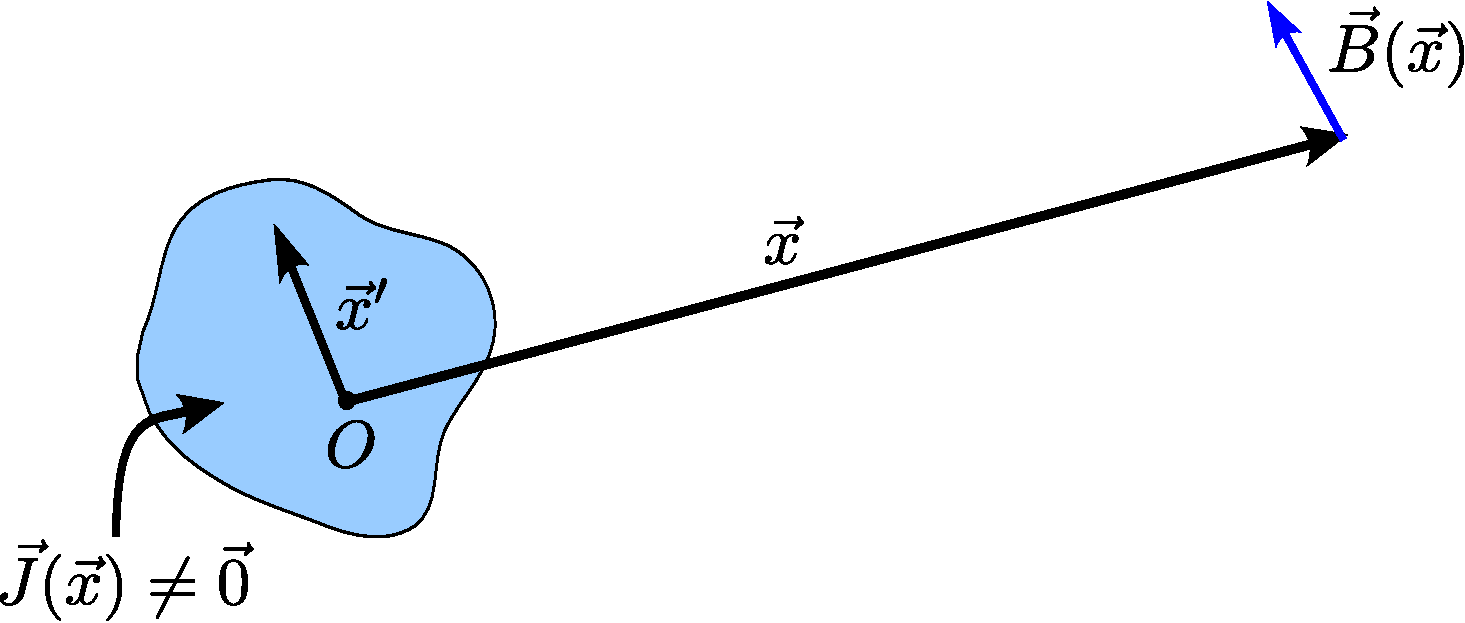
\psfig{file=fig/fig-expansion-multipolar-magnetica-01.pdf,height=4cm,
angle=0 } }
\caption{Esquema de la expansi'on multipolar magn'etica.}
\label{MM1}
\end{figure}
An'alogamente al caso electrost'atico, deseamos calcular el campo
magn'etico $\vec{B}$ lejos de una distribuci'on  de corrientes, descritas por una densidad de corriente $\vec{J}$, localizada en una regi'on peque\~na comparada con la distancia a la cual se calcular'a el campo.

Situando el origen en un punto representativo de la distribuci'on de
corrientes, tendremos que para distancias grandes comparadas con el
tama\~no de la distribuci'on se satisface $\left\vert\vec{x}\right\vert \gg\left\vert
\vec{x}'\right\vert $,\ ver figura \ref{MM1}. Con esto, podemos usar la
expansi'on (\ref{exp1or}) y reescribir la expresi'on (\ref{defA}) como una
expansi'on multipolar magn'etica:
\begin{equation}
 A_i(x)=\frac{\mu_0}{4\pi}\sum_{n=0}^\infty \frac{(-1)^n}{n!}M_{i_1\cdots
i_ni}\partial_{i_1}\cdots \partial_{i_n}\frac{1}{r},
\end{equation}
donde hemos definidos los \textbf{momentos multipolares magn'eticos} como
\begin{equation}
\boxed{ M_{i_1\cdots i_ni}:=\int_V x_{i_1}\cdots x_{i_n}\,J_i(x)\,dV.}
\end{equation}
Note que, debido al caracter vectorial de la densidad de corriente, el momento
multipolar magn'etico de orden $n$ es un tensor de orden $n+1$.

En la pr'actica es com'un usar s'olo los primeros t'erminos de la expansi'on
multipolar magn'etica. Adem'as, el t'ermino monopolar magn'etico es siempre
identicamente nulo \textit{para corrientes estacionarias}, ya que
\begin{equation}
 M_i=\int_V J_i(x)\,dV=0. \label{mmm0}
\end{equation}
Para probar esto, considere la siguiente integral $\oint_{\partial V}x_i
J_j\,dS_j$. Usando el teorema de Gauss podemos escribir
\begin{equation}
 \oint_{\partial V}x_i
J_j\,dS_j=\int_V\partial_j(x_iJ_j)\,dV=\int_V\left[
(\partial_jx_i)J_j+x_i(\partial_jJ_j)\right]\,dV=\int_V\left[
\delta_{ij}J_j+0\right]\,dV
\end{equation}
En la 'ultima igualdad usamos el hecho que para corrientes estacionarias la
divergencia del vector densidad de corriente es nula, ver \eqref{divJ0}. Con esto, encontramos la
identidad
\begin{equation}
  \int_VJ_i\,dV\equiv \oint_{\partial V}x_iJ_j\,dS_j.
\end{equation}
Esta identidad es v'alida para cualquier volumen $V$. Entonces para probar lo
requerido basta considerar un volumen que \textit{contiene totalmente}
la distribuci'on de corrientes, de modo que $\vec{J}=\vec{0}$ en la superficie
$\partial V$.

Este resultado general (para corrientes estacionarias) tiene como consecuencia
que \textit{la expansi'on multipolar magn'etica comienza con el t'ermino
dipolar} ($n=1$).

El momento multipolar de orden 1 es dado por
\begin{equation}
 M_{ij}=\int_V x_i\,J_j(x)\,dV.
\end{equation}

Es posible probar que este tensor es \textit{antisim'etrico},
$M_{ij}=-M_{ji}$, \textit{para distribuciones de corrientes estacionarias}. Para esto,
basta analizar la integral $\oint_{\partial V}x_i x_j J_k\,dS_k$ de forma
an'aloga a lo discutido anteriormente, es decir, aplicando el teorema de Gauss y la
condici'on de divergencia nula de la densidad de corriente. Ya que $M_{ij}$ es
antisim'etrico, \textit{la informaci'on que este tensor contiene puede ser
equivalentemente descrita en t'erminos de un (pseudo-) vector} $\vec{\mu}$,
llamado \textbf{momento (dipolar) magn'etico}, y definido por
\begin{equation}
 \mu_i:=\frac{1}{2}\varepsilon_{ijk}M_{jk}, \qquad
M_{ij}=\varepsilon_{ijk}\mu_k, \label{vmdm}
\end{equation}
es decir,
\begin{equation}
 \boxed{\mu_i=\frac{1}{2}\varepsilon_{ijk}\int_V x_j J_k(x)\, dV,}
\end{equation}
o, en notaci'on vectorial, 
\begin{equation}
 \boxed{\vec{\mu}=\frac{1}{2}\int_V \vec{x}\times\vec{J}(x)\,dV,}
\end{equation}
Con esto, el t'ermino dipolar de la expansi'on multipolar magn'etica para el
potencial vectorial \eqref{defA} es
\begin{eqnarray}
 A_i^{(1)}(x)&=&-\frac{\mu_0}{4\pi}M_{ji}\partial_j\frac{1}{r} \\
&=&-\frac{\mu_0}{4\pi}\left(\varepsilon_{jil}\mu_l\right)\left(-\frac{x_j}{
r^3}\right) \\
&=&\frac{\mu_0}{4\pi}\varepsilon_{ijk}\frac{\mu_jx_k}{r^3},
\end{eqnarray}
es decir,
\begin{equation}
 \boxed{\vec{A}^{(1)}(x)=\frac{\mu_0}{4\pi}\frac{\vec{\mu}\times\vec{x}}{r^3}.}
\label{Adip}
\end{equation}
M'as importante que el potencial, que sabemos no es 'unico, es el campo
magn'etico. La contribuci'on dipolar al campo generado por una distribuci'on
compacta de corriente es entonces dado por
\begin{eqnarray}
B_i^{(1)}(x)&=&\varepsilon_{ijk}\partial_jA_k^{(1)}(x)\\
&=&\varepsilon_{ijk}\partial_j\left(\frac{\mu_0}{4\pi}\varepsilon_{klm}\frac{
\mu_lx_m}{r^3}\right) \\
&=&\frac{\mu_0}{4\pi}\varepsilon_{ijk}\varepsilon_{klm}\mu_l\partial_j\left(
\frac{x_m}{r^3}\right) \\
&=&\frac{\mu_0}{4\pi}\left(\delta_{il}\delta_{jm}-\delta_{jl}\delta_{im}\right)
\mu_l\left(\frac{\delta_{jm}}{r^3}-3\frac{x_mx_j}{r^5}\right) \\
&=&\frac{\mu_0}{4\pi}\left[3\frac{x_i(x_j\mu_j)}{r^5}-\frac{\mu_i}{r^3}
\right] ,
\end{eqnarray}
o, en notaci'on vectorial
\begin{equation}
\boxed{\vec{B}^{(1)}=\frac{\mu_0}{4\pi}\left[\frac{3\hat{r}(\vec{\mu}
\cdot\hat{r}) -\vec{\mu}}{r^3}\right] , \qquad \hat{r}:=\frac{\vec{x}}{r}.}
\end{equation}
\begin{figure}[!h]
\centerline{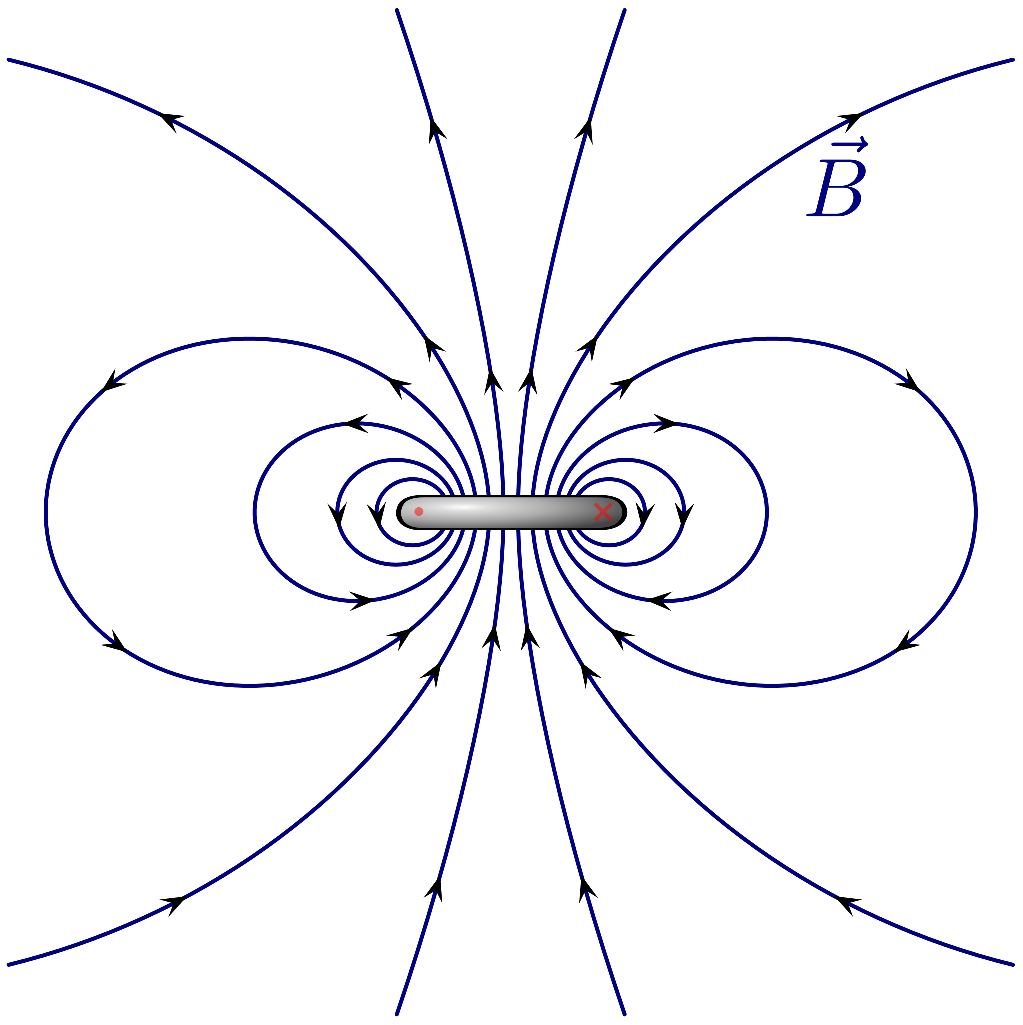
\psfig{file=fig/fig-campo-magnetico-espira.pdf,height=5cm,angle=0}\hspace{2cm}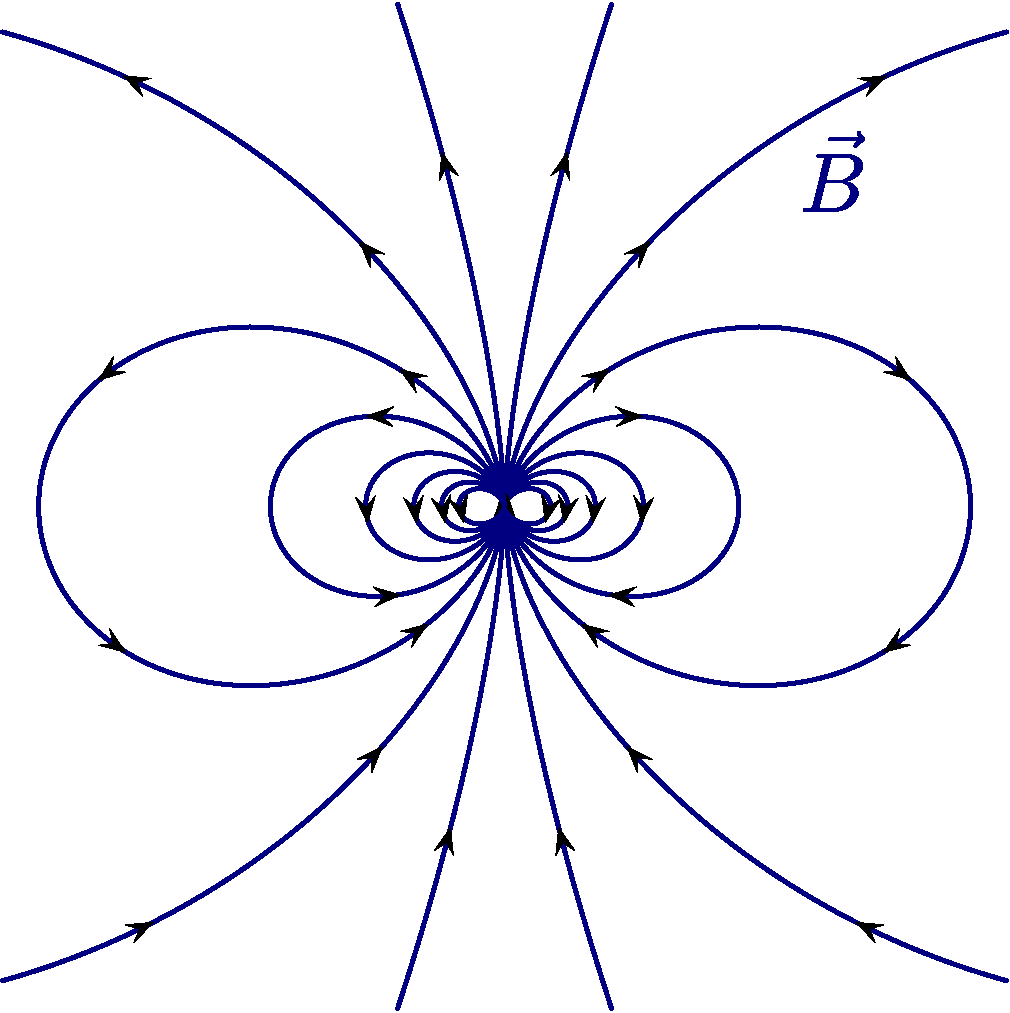
\psfig{file=fig/fig-campo-dipolo-magnetico.pdf,height=5cm,angle=0}}
\caption{a) Campo magn'etico de una espira, b) campo magn'etico de un dipolo ideal. Adaptadas a partir de \href{http://commons.wikimedia.org/wiki/File:VFPt_dipole_point.svg}{esta} y \href{http://commons.wikimedia.org/wiki/File:VFPt_dipole_magnetic3.svg}{esta} figuras originales.}
\label{fig:dipmag}
\end{figure}

\subsection{Momento dipolar de una espira plana}
\begin{figure}[!h]
\centerline{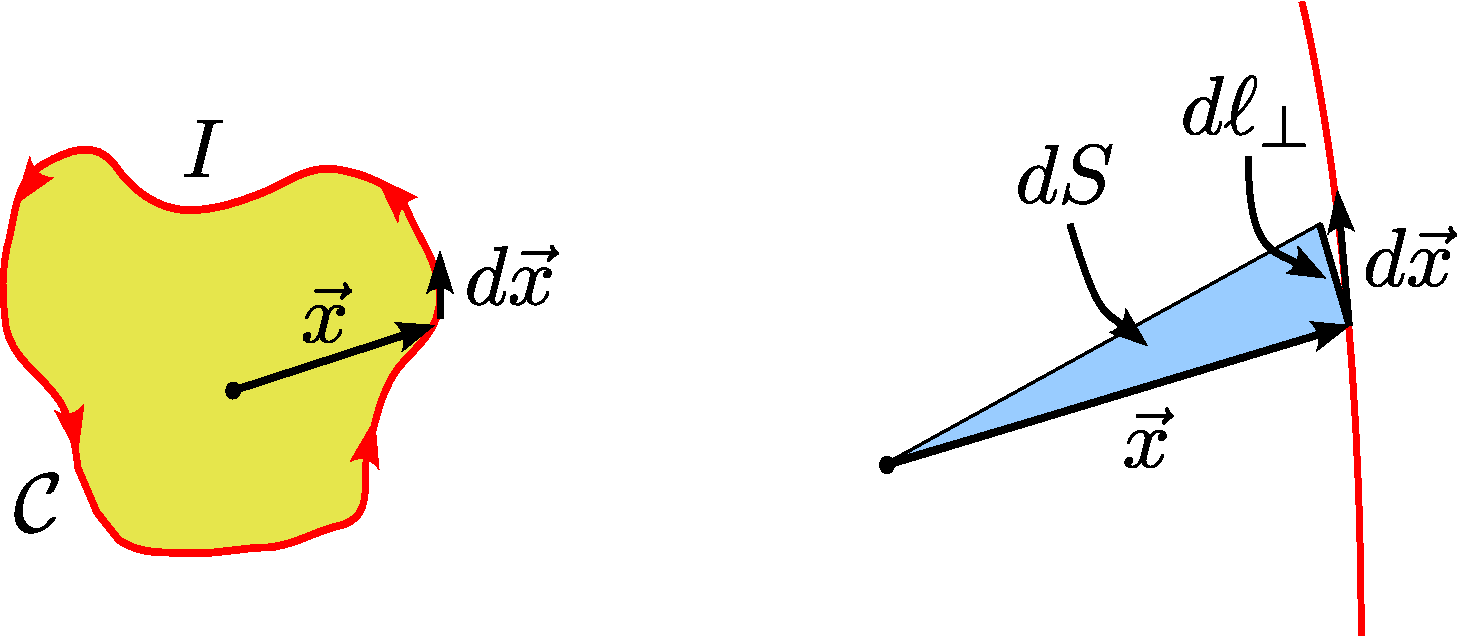
\psfig{file=fig/fig-espira-plana-01.pdf,height=4cm,angle=0}}
\caption{Espira plana y elemento de 'area.}
\label{fep01}
\end{figure}
En el caso de que la distribuci'on de corriente se concentre en conductores que
describen una curva $\cal C$ (sobre un plano) y transportan corriente $I$, el momento magn'etico
es dado por
\begin{equation}\label{muintC}
 \vec{\mu}=\frac{I}{2}\oint_{\cal C} \vec{x}\times d\vec{x}.
\end{equation}
En el caso de un \textit{espira plana}, pero de forma arbitraria, tenemos que
(situando el origen en un punto del mismo plano), $\vec{x}\times
d\vec{x}/2=rd\ell_\bot\hat{n}/2=dS\,\hat{n}$, donde $\hat{n}$ es el
vector normal a la espira cuya con direcci'on dada por la regla de la mano
derecha aplicada a la curva orientada de acuerdo al sentido de circulaci'on de
la corriente\footnote{Equivalentemente, puede obtener este resultado a partir de \eqref{muintC} usando el teorema de Stokes.}. Con esto obtenemos que el momento magn'etico de una espira plana
de 'area $A$ es siempre de la forma
\begin{equation}\marginnote{Momento magn'etico espira plana}
 \boxed{\vec{\mu}=IA\,\hat{n}.}
\end{equation}

\subsection{Relaci'on entre momento magn'etico y momento angular}
En algunos sistemas se tiene que la densidad de carga el'ectrica (en cada
punto) es proporcional a la densidad de masa, de modo que
\begin{equation}
 \rho(x)=\frac{Q}{M} \rho_{\rm m}(x).
\end{equation}
donde $Q$ es la carga total y $M$ la masa total del sistema. Esto ocurre, en
general, en sistemas constituidos por \textit{un s'olo tipo de part'iculas},
masivas y cargadas. En este caso, si cada elemento del sistema se mueve
con velocidad $\vec{v}(x)$, entonces
\begin{equation}
\vec{J}=\rho(x)\vec{v}(x)=\frac{Q}{M} \rho_{\rm m}(x)\vec{v}(x)
\end{equation}
y entonces el momento magn'etico puede escribirse como
\begin{equation}
 \vec{\mu}=\frac{1}{2}\int_V \vec{x}\times\vec{J}\,dV=\frac{Q}{2M}\int_V
\vec{x}\times\rho_{\rm m}(x)\vec{v}(x)\,dV=\frac{Q}{2M}\int_V
\vec{x}\times d\vec{p},
\end{equation}
donde $d\vec{p}:=\rho_{\rm m}(x)\vec{v}(x)\,dV$ denota el \textbf{momentum lineal} de la masa en el elemento de volumen $dV$. De esta forma $d\vec{L}:=\vec{x}\times d\vec{p}$ es el \textbf{momento angular} del peque\~no elemento de masa (respecto al origen elegido) y, finalmente,
\begin{equation}
 \boxed{\vec{\mu}=\frac{Q}{2M}\vec{L}.}
\end{equation}

\section{Fuerza y torque sobre una distribuci'on compacta de corriente}
Consideramos ahora el caso en que una peque\~na distribuci'on de corriente
se ubica en una regi'on donde existe un campo magn'etico \textit{externo}
$\vec{B}(x)$.

La fuerza total que la distribuci'on de corrientes experimenta, debido al campo
externo (es decir, sin tomar en cuenta la autointeracci'on de la distribuci'on),
es dada por (\ref{fm1}). Para expresar esta fuerza en t'erminos de los momentos multipolares magn'eticos de la distribuci'on, situamos nuevamente el
origen de coordenadas en un punto representativo de la distribuci'on y expandimos la
intensidad de campo magn'etico en puntos dentro de 'esta en una serie
de potencias de las componentes del $\vec{x}'$:
\begin{align}
 B_i(\vec{x}+\vec{x}') &= \sum_{n=0}^\infty \frac{1}{n!}x'_{i_1}\cdots x'_{i_n}(\partial_{i_1}\cdots\partial_{i_n}B_i)(x) \label{expB} \\
 &= B_i(x)+x'_j(\partial_jB_i)(x) +
\frac{1}{2}x'_jx'_k(\partial_j\partial_kB_i)(x)+\cdots .
\end{align}
Reemplazando esto en (\ref{fm1}), y tomando en cuenta que la integral sobre la regi'on con corrientes es sobre la variable $\vec{x}'$, encontramos
\begin{align}
F^{\rm m}_i &=  \varepsilon_{ijk}\sum_{n=0}^\infty\frac{1}{n!}M_{i_1\cdots i_nj}(\partial_{i_1}\cdots\partial_{i_n}B_k)(x)\\
&= \varepsilon_{ijk}\left[M_jB_k(x)+M_{lj}(\partial_lB_k)(x)+\frac{1}{2}M_{lnj}(\partial_l\partial_nB_k)(x) +\cdots\right].
\end{align}
Usando (\ref{mmm0}) y (\ref{vmdm}) obtenemos
\begin{eqnarray}
F^{\rm m}_i
&=&\varepsilon_{ijk}\varepsilon_{ljm}\,\mu_m (\partial_lB_k)(x)+\cdots \\
&=& \mu_j(\partial_iB_j)(x)-\mu_i(\partial_jB_j)(x)+\cdots .
\end{eqnarray}
Finalmente, usando la ecuaci'on de campo (\ref{divB}) llegamos a
\begin{equation}
 \boxed{F^{\rm m}_i=\mu_j(\partial_iB_j)(x)+\cdots .}
\end{equation}
En otras palabras, la primera contribuci'on en la expansi'on multipolar a la
fuerza neta sobre una distribuci'on arbitraria es dada por el t'ermino dipolar,
con
\begin{equation}
 \boxed{F_i^{\rm m,(1)}=-\partial_i U_{\rm m}, }
\end{equation}
donde hemos introducido la \textbf{energ'ia de interacci'on entre un dipolo magn'etico
y un campo externo}
\begin{equation}
 \boxed{U_{\rm m}(x)=-\vec{\mu}\cdot\vec{B}(x).} \label{Umagdip}
\end{equation}

Similarmente, el torque neto sobre la espira (con respecto al punto de referencia $O$)  puede calcularse a partir de
\begin{equation}
 \tau_i=\varepsilon_{ijk}\int_V x'_j f^{\rm m}_k(x') dV',
\end{equation}
donde $f^{\rm m}_k$ son las componentes de la densidad de fuerza magn'etica,
definida en (\ref{dfm}). Por lo tanto, usando nuevamente la expansi'on
(\ref{expB}) podemos escribir,
\begin{eqnarray}
  \tau_i&=&\varepsilon_{ijk}\varepsilon_{kln}\int_V x'_j J_l(x')B_n(x')\, dV' \\
&=&\varepsilon_{ijk}\varepsilon_{kln}\int_V x'_j
J_l(x')\left[B_n(x)+x'_p(\partial_pB_n)_(x) +\cdots\right] dV \\
&=&\varepsilon_{ijk}\varepsilon_{kln}\left[M_{jl}B_n(x)+M_{jpl}(\partial_pB_n)(x)
+\cdots\right] \\
&=&\varepsilon_{ijk}\varepsilon_{kln}\varepsilon_{jlp}\,\mu_pB_n(x)+\cdots\\
&=&\varepsilon_{ijk}\,\mu_jB_k(x)+\cdots 
\end{eqnarray}
o, en notaci'on vectorial
\begin{equation}
 \boxed{\vec{\tau}=\vec{\mu}\times\vec{B}+\cdots .} \label{torqueB}
\end{equation}
Puede verificarse usando (\ref{Umagdip}) y (\ref{torqueB}) que un dipolo
magn'etico (o, en primera aproximaci'on, toda distribuci'on compacta de
corriente) situado en un campo (homog'eneo) externo experimentar'a un torque
que tender'a a \textit{alinear} el momento magn'etico de la distribuci'on con el
del campo externo. La posici'on de equilibrio corresponde al caso en que
$\vec{\mu}$ es paralelo a $\vec{B}$, que es adem'as un equilibrio estable ya
que la energ'ia de interacci'on es m'inima. M'as generalmente, el momento
magn'etico puede realizar un \textbf{movimiento de precesi'on} en torno al campo
magn'etico.

%\subsection{Ejemplo: Precesi'on de Larmor}

\section{Campos magn'eticos en la materia}
An'alogamente al caso electrost'atico, en el que un medio se polariza en
presencia de un campo externo, 'este puede adem'as \textit{magnetizarse}. Esto
significa que en cada peque\~no elemento de volumen (macrosc'opico) puede existir un momento magn'etico no nulo. Este momento magn'etico puede ser producto de
los peque\~nos ``loops''\, de corrientes inducidas por el campo aplicado sobre los
electrones at'omicos. Este tipo de dipolos se inducen en \textit{direcci'on contraria}
al campo aplicado, por lo que tienden a \textit{reducir} el valor de la inducci'on
magn'etica al interior del material. Los materiales \textbf{diamagn'eticos} son aquellos en que este tipo de magnetizaci'on es dominante. El hecho que las
part'iculas subat'omicas, y en particular los electrones, posean \textit{momentos
magn'eticos intr'insecos} (permanentes), hace posible que un material presente
magnetizaci'on no nula, de origen distinto a la generada por las corrientes
inducidas. En general, un campo magn'etico aplicado tender'a a alinear, en
mayor o menor medida, los momentos magn'eticos permanentes del material con el campo aplicado, pudiendo compensar y revertir la magnetizaci'on debida a las corrientes
inducidas. Los materiales paramagn'eticos presentan momentos magn'eticos
netos en la misma direcci'on del campo aplicado. En los ferromagnetos, por
otro lado, la alineaci'on de los momentos magn'eticos permanentes es tal que el
momento magn'etico total es no nulo en ausencia de un campo aplicado, y puede asumir valores varios ordenes de magnitud mayor que el caso de los paramagnetos.

\subsection{Magnetizaci'on}
En resumen, consideraremos que en el interior de un medio, existen momentos
magn'eticos distribuidos en su interior. Modelaremos esta distribuci'on
definiendo el \textbf{(pseudo-)vector de magnetizaci'on} como la densidad de momento
magn'etico, es decir, como el momento magn'etico por unidad de volumen en una
peque\~na regi'on ($\Delta V\to 0$, desde el punto de vista macrosc'opico) del
material:
\begin{equation}\marginnote{Definici'on Magnetizaci'on}
\vec{M}(x):= \lim_{\Delta V\to 0} \frac{\Delta \vec{\mu}}{\Delta V}.
\end{equation}
Como consecuencia, la magnetizaci'on tiene unidades de corriente por unidad de
longitud: $[\vec{M}]={[\vec{\mu}]}/{L^3}={IL^2}/{L^3}={I}/{L}$.
Con esta definici'on, tenemos que el momento magn'etico $d\vec{\mu}(x)$
contenido en un elemento de volumen (macrosc'opico) $dV$ centrado en un punto con  posici'on
$\vec{x}$ es
\begin{equation}
d\vec{\mu}(x)=\vec{M}(x)\,dV.
\end{equation}
Entonces, a partir de (\ref{Adip}) podemos calcular al campo (potencial
vectorial) producido por la distribuci'on de momentos dipolares como la
superposici'on del campo correspondiente al momento dipolar magn'etico contenido en cada
elemento de volumen:
\begin{eqnarray}
 A_i^{\rm M}(x)&=&\frac{\mu_0}{4\pi}\varepsilon_{ijk}\int_V
\frac{d\mu_j(x')(x_k-x'_k)}{ \left\vert\vec{x} -\vec{x}'\right\vert^3} \\
&=& \frac{\mu_0}{4\pi}\varepsilon_{ijk}\int_V \frac{M_j(x')(x_k-x'_k)}{
\left\vert\vec{x} -\vec{x}'\right\vert^3}dV'.
\end{eqnarray}
Usando la identidad (\ref{id01}) podemos escribir este potencial vectorial
producido por la magnetizaci'on del material como:
\begin{eqnarray}
  A_i^{\rm M}(x)&=& \frac{\mu_0}{4\pi}\varepsilon_{ijk}\int_V
M_j(x')\partial'_k\frac{1}{\left\vert\vec{x} -\vec{x}'\right\vert}dV'
\label{AM1}\\
&=& \frac{\mu_0}{4\pi}\varepsilon_{ijk}\int_V\left[\partial'_k\left(
\frac{M_j(x')}{\left\vert\vec{x}
-\vec{x}'\right\vert}\right)-\frac{(\partial'_kM_j(x'))}{\left\vert\vec{x}
-\vec{x}'\right\vert}\right]dV' \\
&=&\frac{\mu_0}{4\pi}\oint_{\partial
V}\frac{\varepsilon_{ijk}M_j(x')}{\left\vert\vec{x}
-\vec{x}'\right\vert}dS'_k+\frac{\mu_0}{4\pi}\int_V\frac{(\varepsilon_{ijk}
\partial'_jM_k(x'))}{ \left\vert\vec{x}-\vec{x}'\right\vert}dV' \\
&=&\frac{\mu_0}{4\pi}\oint_{\partial
V}\frac{(\varepsilon_{ijk}M_j(x')\hat{n}_k)}{\left\vert\vec{x}
-\vec{x}'\right\vert}dS'+\frac{\mu_0}{4\pi}\int_V\frac{(\varepsilon_{ijk}
\partial'_jM_k(x'))}{ \left\vert\vec{x}-\vec{x}'\right\vert}dV'  \\
&=&\frac{\mu_0}{4\pi}\oint_{\partial
V}\frac{j^{\rm M,S}_i(x')}{\left\vert\vec{x}
-\vec{x}'\right\vert}dS'+\frac{\mu_0}{4\pi}\int_V\frac{J^{\rm M}_i(x')}{
\left\vert\vec{x}-\vec{x}'\right\vert}dV'.
\end{eqnarray}
En resumen
\begin{equation}
 \boxed{\vec{A}^{\rm M}(x)=\frac{\mu_0}{4\pi}\int_V\frac{\vec{J}^{\rm M}(x')}{
\left\vert\vec{x}-\vec{x}'\right\vert}dV'+\frac{\mu_0}{4\pi}\oint_{\partial
V}\frac{\vec{j}^{\rm M}(x')}{\left\vert\vec{x}-\vec{x}'\right\vert}dS',}
\label{AM01}
\end{equation}
donde hemos definido la \textbf{densidad de corriente de magnetizaci'on}
$\vec{J}^{\rm M}$ y la \textbf{densidad de corriente superficial de
magnetizaci'on} $\vec{j}^{\rm M}$ por
\begin{equation}\marginnote{corrientes de magnetizaci'on}
\boxed{\vec{J}^{\rm M}(x):=\vec\nabla\times\vec{M}(x), \qquad \vec{j}^{\rm
M}(x):=\vec{M}(x)\times\hat{n}(x).}
\end{equation}
Estas definiciones de densidades de corriente, que pueden ser reales o
ficticias dependiendo del origen de la magnetizaci'on $\vec{M}$, son de utilidad
puesto que, de acuerdo a (\ref{AM01}), el campo producido por la magnetizaci'on
es \textit{equivalente} al campo producido (a trav'es de la ley de Biot-Savart)
por las corrientes descritas por $\vec{J}^{\rm M}$ en el interior del material y
por $\vec{j}^{\rm M}$ en su superficie.

\begin{figure}[!h]
\centerline{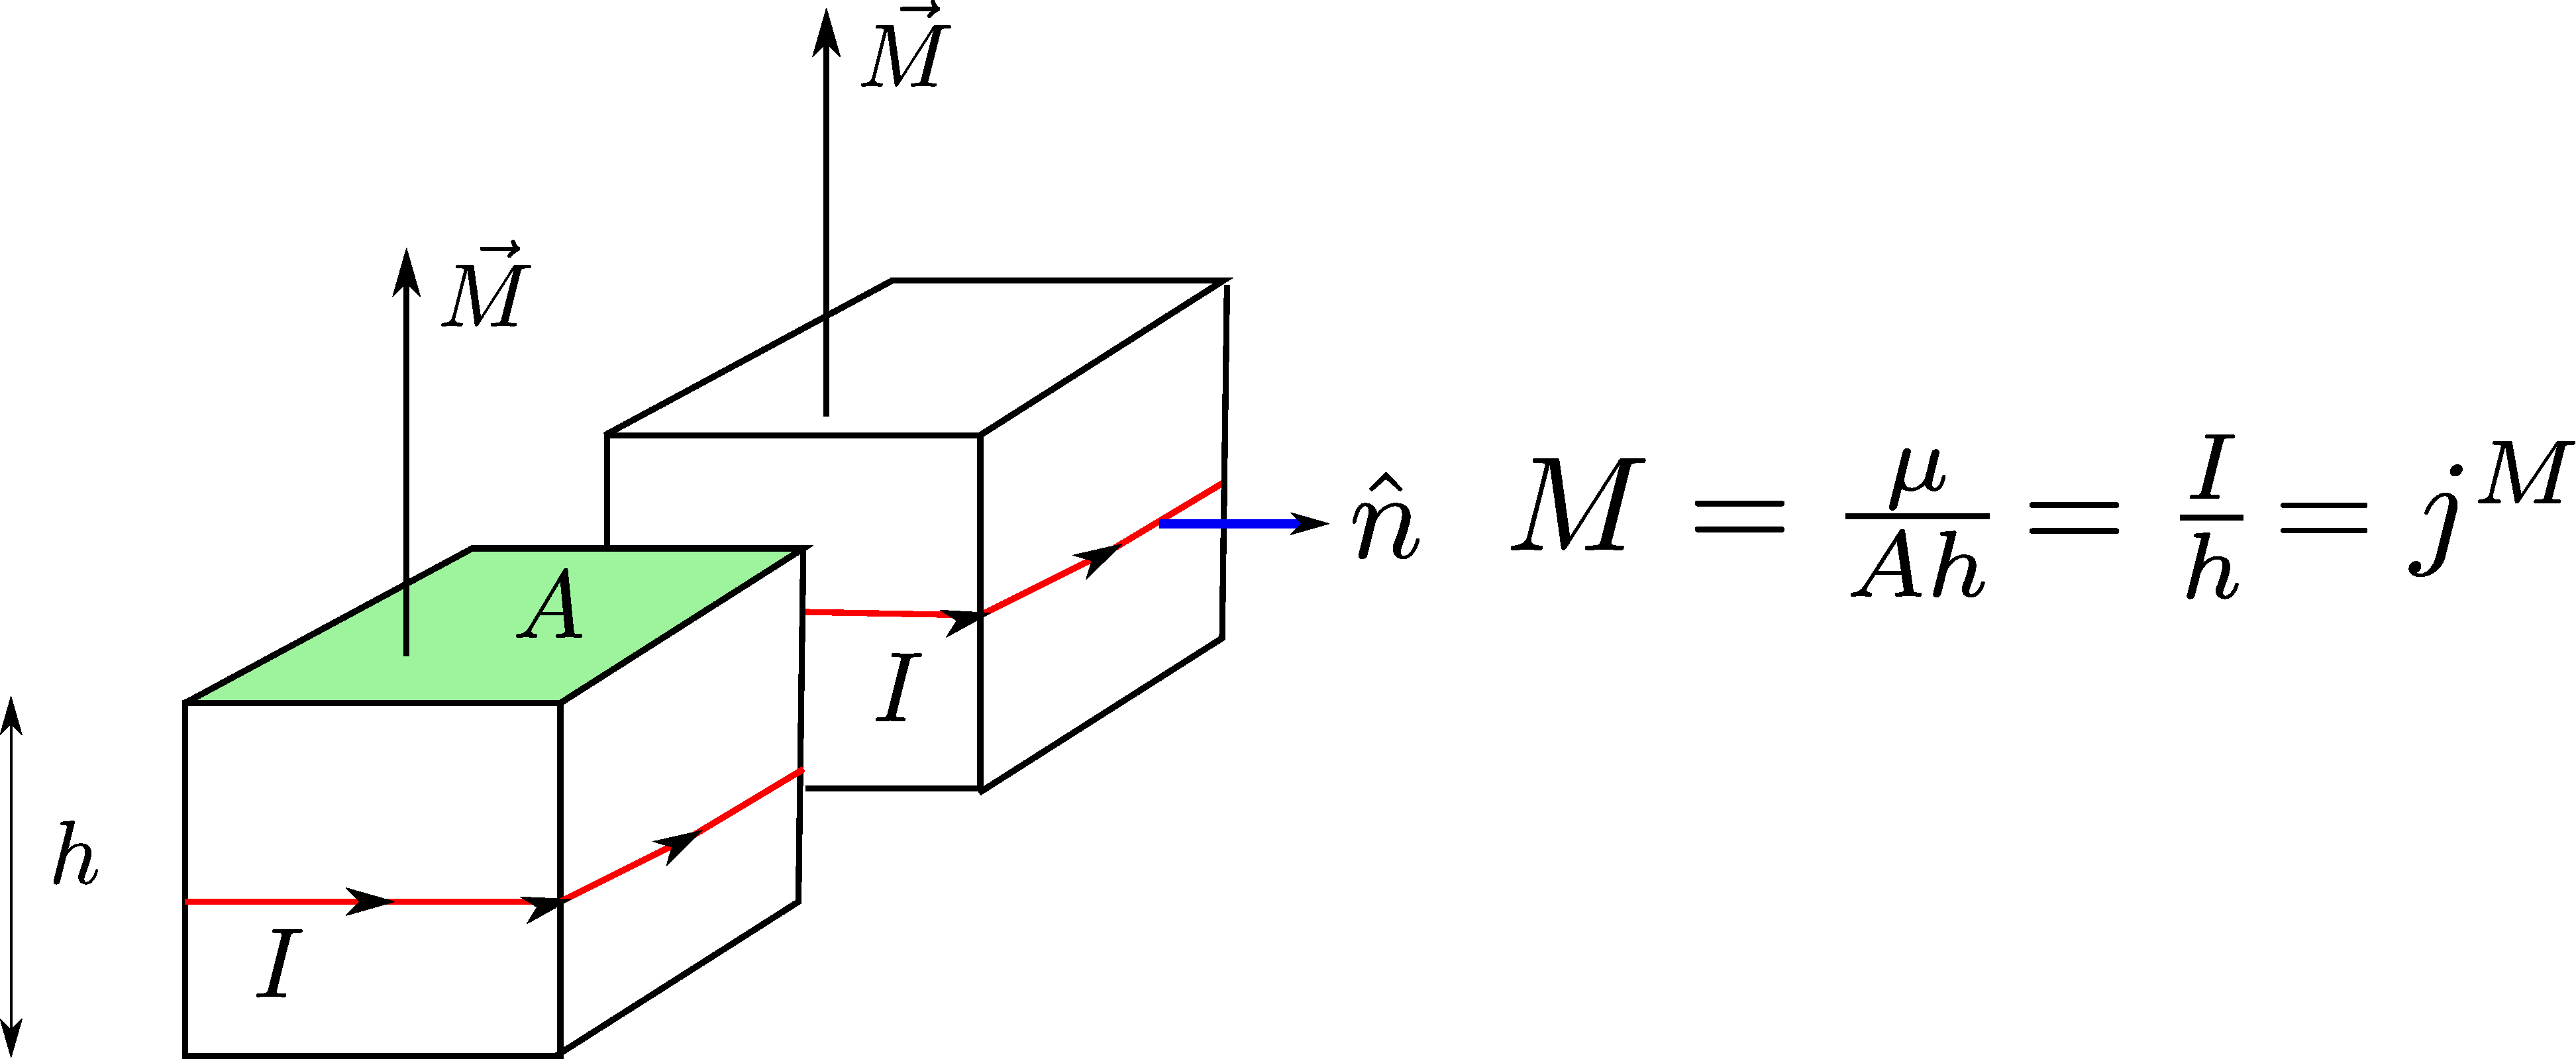
\psfig{file=fig/fig-corriente-magnetizacion-superficie.pdf,height=3cm,angle=0}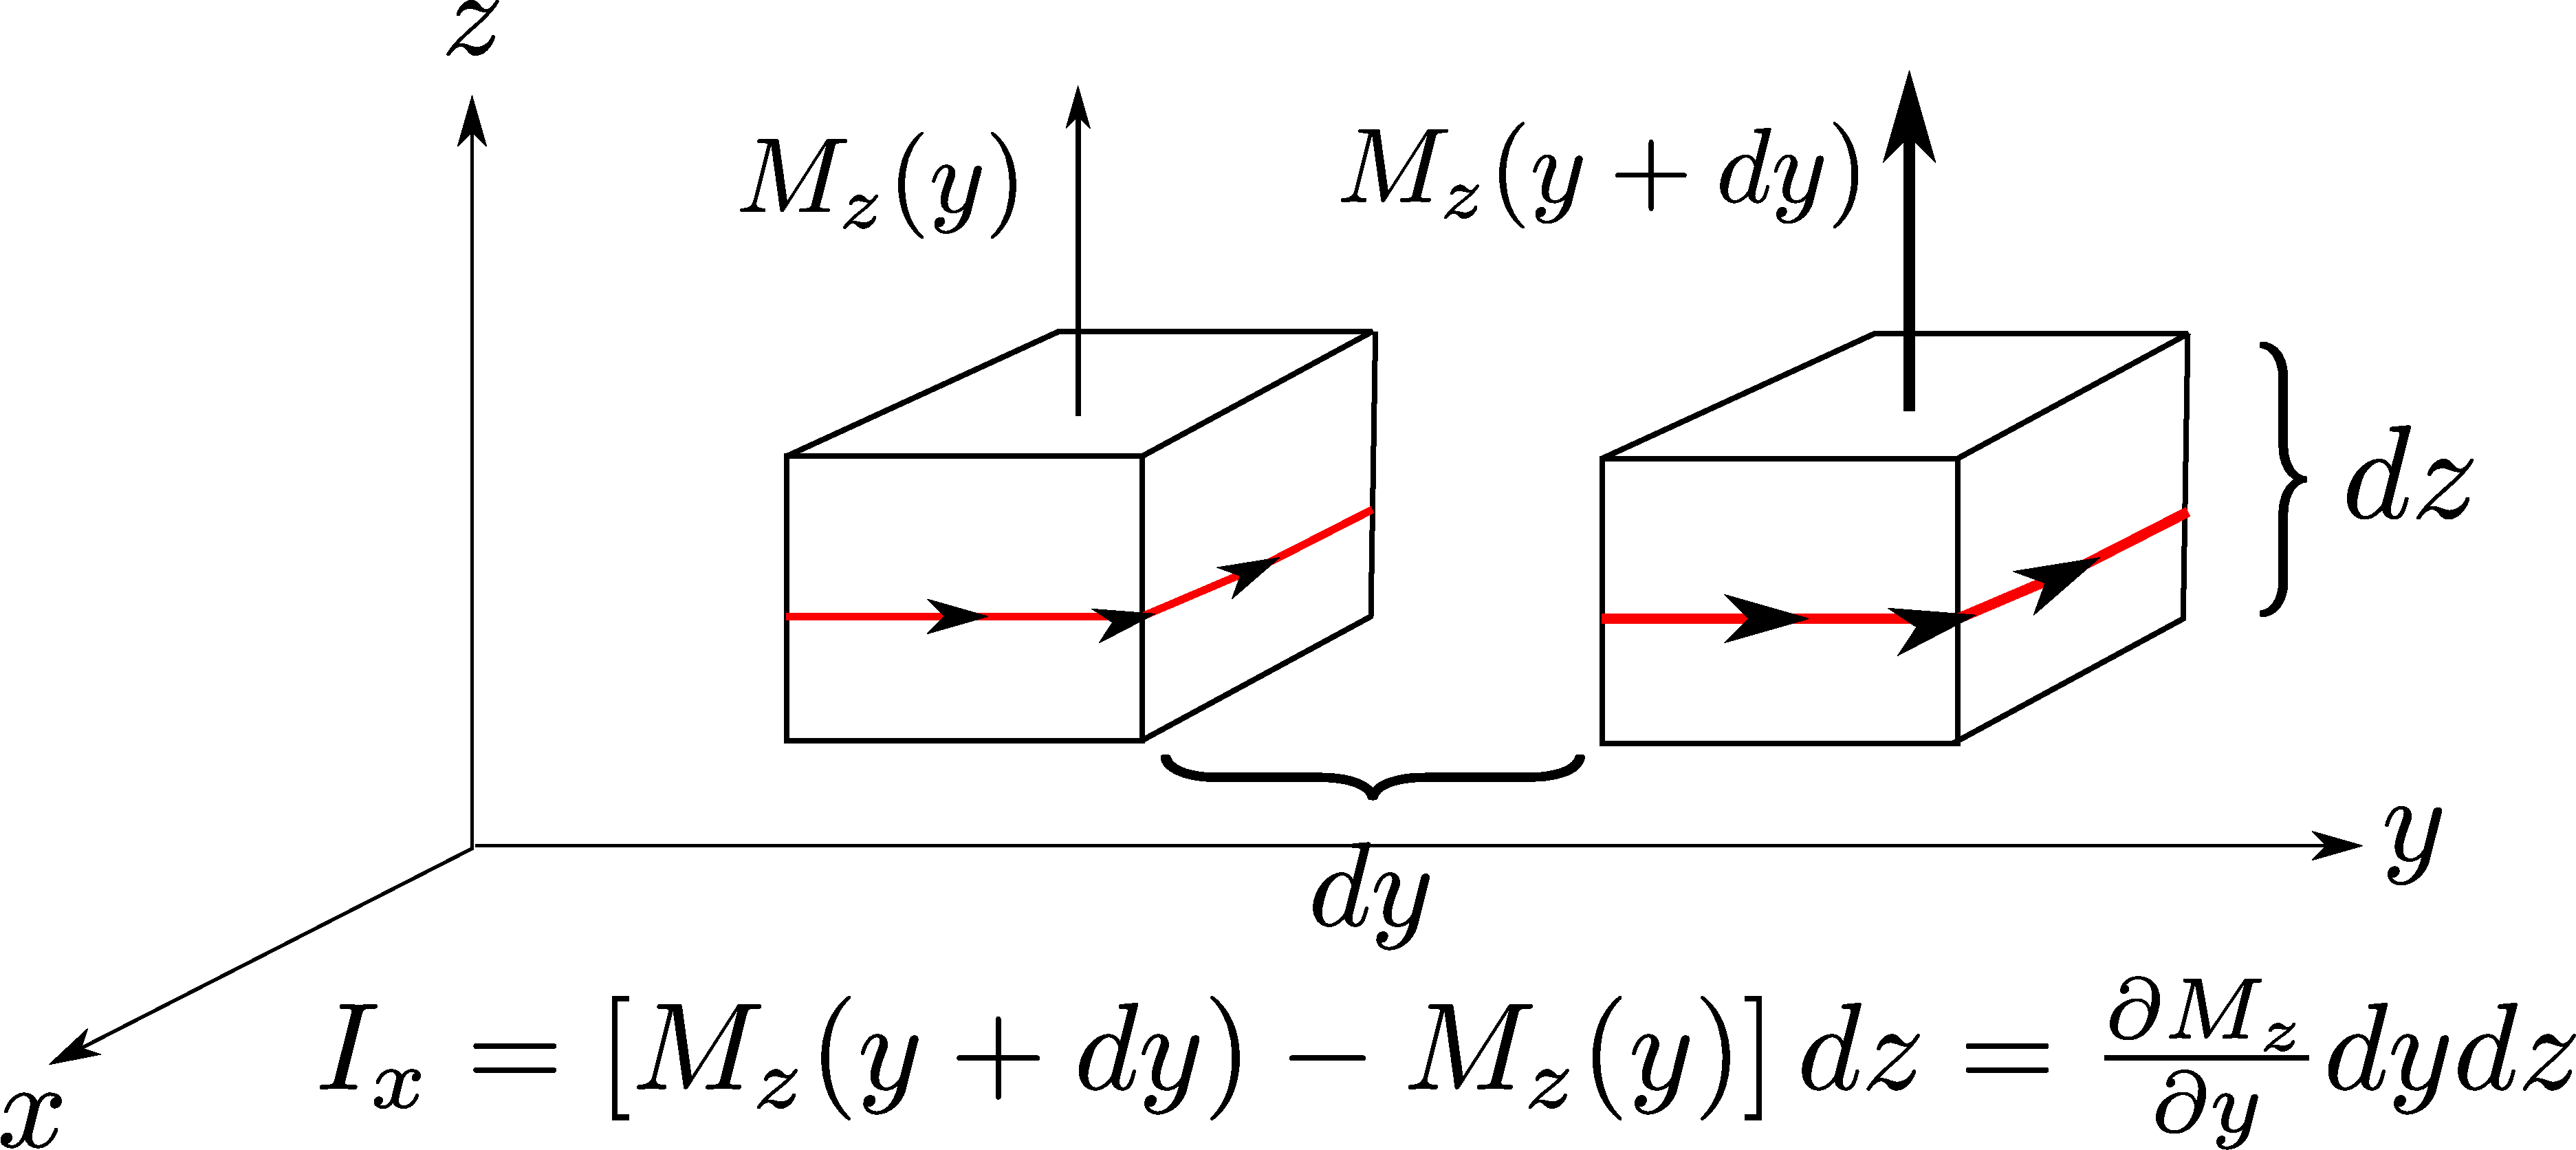
\psfig{file=fig/fig-corriente-magnetizacion-volumen.pdf,height=3cm,angle=0}}
\caption{Corrientes de magnetizaci'on de volumen y superficie. (Figura original gentileza de A. Maldonado) *** EDITAR, MEJORAR, EXPLICAR ***}
\label{fig-corriente-magnetizacion}
\end{figure}

Usando (\ref{AM1}) podemos calcular la contribuci'on de la magnetizaci'on a  la inducci'on magn'etica como:
\begin{eqnarray}
 B_i^{\rm M}&=&\varepsilon_{ijk}\partial_jA_k^{\rm M} \\
&=&\frac{\mu_0}{4\pi}\varepsilon_{ijk}\varepsilon_{kln}\int_V
M_l(x')\partial_j\partial'_n\frac{1}{\left\vert\vec{x}
-\vec{x}'\right\vert}dV'\\
&=&-\frac{\mu_0}{4\pi}\left(\delta_{il}\delta_{jn}-\delta_{in}
\delta_{jl}\right)\int_VM_l(x')\partial_j\partial_n\frac{1}{\left\vert\vec{x}
-\vec{x}'\right\vert}dV'\\
&=&\frac{\mu_0}{4\pi}\int_V\left[M_j(x')\partial_j\partial_i\frac{1}{
\left\vert\vec { x }-\vec{x}'\right\vert}-M_i(x')\partial_j\partial_j\frac{1}{
\left\vert\vec { x }-\vec{x}'\right\vert}\right]dV'\\
&=&\frac{\mu_0}{4\pi}\partial_i\left[\int_VM_j(x')\partial_j\frac{1}{
\left\vert\vec{x}-\vec{x}'\right\vert}dV'\right]-\frac{\mu_0}{4\pi}\int_V
M_i(x')\nabla^2\frac{1} {\left\vert\vec {x}-\vec{x}'\right\vert}dV'\\
&=&-\frac{\mu_0}{4\pi}\partial_i\left[\int_VM_j(x')\partial'_j\frac{1}{
\left\vert\vec{x}-\vec{x}'\right\vert}dV'\right]+\mu_0\int_V
M_i(x')\delta^{(3)}(\vec{x}-\vec{x}')dV',
\end{eqnarray}
de donde obtenemos:
\begin{equation}
 \boxed{\vec{B}^{\rm M}(x)=\mu_0\vec{M}(x)-\mu_0\vec\nabla\phi^*_{\rm M}(x),}
\label{BM}
\end{equation}
donde hemos definido el \textbf{potencial escalar de magnetizaci'on}\footnote{Note que 'este es un campo \textit{distinto} al potencial escalar magn'etico definido en la secci'on \ref{secpem}.}
\begin{equation}\marginnote{Potencial escalar de magnetizaci'on}
 \boxed{\phi^*_{\rm M}(x):=\frac{1}{4\pi}\int_VM_j(x')\partial'_j\frac{1}{
\left\vert\vec{x}-\vec{x}'\right\vert}dV'=\frac{1}{4\pi}
\int_V\frac{\vec{M}(x')\cdot (\vec{x}-\vec{x}')}{\left\vert\vec{x}-\vec{x}
'\right\vert^3} dV'. }
\end{equation}
En un sistema general existir'an, adem'as de la magnetizaci'on, corrientes
\textit{externas} (tambi'en llamadas \textit{libres} o \textit{de transporte}),
por lo que la inducci'on magn'etica total es dada por:
\begin{equation}
 \vec{B}(x)=\vec{B}^{\rm ext}(x)+\vec{B}^{\rm M}(x) .
\end{equation}
Usando (\ref{BS2}) y (\ref{BM}) encontramos finalmente una expresi'on para 
la inducci'on magn'etica macrosc'opica total en un medio magnetizado y con
corrientes externas:
\begin{equation}\marginnote{$\vec{B}$: corrientes externas + magnetizaci'on}
\boxed{ \vec{B}(x)=\frac{\mu_0}{4\pi}\int_V\frac{\vec{J}_{\rm ext}
(x')\times\left(\vec{x}-\vec{x}'\right)}{\left\vert\vec{x}-\vec{x}'\right\vert^3
} dV' +\mu_0\vec{M}(x)-\mu_0\vec\nabla\phi^*_{\rm M}(x).}
\label{BMG}
\end{equation}

\subsection{Excitaci'on magn'etica}\label{sec:defH}
Al calcular el rotor del campo definido en (\ref{BMG}), vea (\ref{ley-Ampere}),
encontramos:
\begin{equation}
 \vec\nabla\times\vec{B}=\mu_0\,\vec{J}_{\rm ext}
+\mu_0\vec\nabla\times\vec{M}.
\end{equation}
De aqu'i, podemos escribir
\begin{equation}
 \vec\nabla\times\left(\frac{1}{\mu_0}\vec{B}-\vec{M}\right)=\vec{J}_{
\rm ext}.
\end{equation}
Esto motiva definir la \textbf{excitaci'on magn'etica} (tambi'en llamada
\textbf{intensidad de campo magn'etico}):
\begin{equation}\marginnote{Excitaci'on magn'etica}\label{defH}
\boxed{\vec{H}(x):=\frac{1}{\mu_0}\vec{B}(x)-\vec{M}(x),}
\end{equation}
es decir,
\begin{equation}\label{HJM}
\vec{H}(x):=\frac{1}{4\pi}\int_V\frac{\vec{J}_{\rm ext}
(x')\times\left(\vec{x}-\vec{x}'\right)}{\left\vert\vec{x}-\vec{x}'\right\vert^3
} dV' -\vec\nabla\phi^*_{\rm M}(x) ,
\end{equation}
que satisface entonces la ``ley de Amp\`ere'',
\begin{equation}\marginnote{L. de Amp\`ere para $\vec{H}$}
 \boxed{\vec\nabla\times\vec{H}=\vec{J}_{\rm ext}} \label{rotHj}
\end{equation}
o, en su versi'on integral,
\begin{equation}
 \boxed{\oint_{\cal C}\vec{H}\cdot d\vec\ell=I_{\rm ext} .} \label{intHI}
\end{equation}
An'alogamente al caso del vector de desplazamiento el'ectrico $\vec{D}$, la
intensidad de campo magn'etico $\vec{H}$ es una cantidad 'util puesto que est'a
relacionada, a trav'es de la ecuaci'on (\ref{rotHj}), con las corrientes
externas del sistema, que son las corrientes que (en principio) pueden ser
manipuladas.

A partir de (\ref{HJM}) vemos que \textit{en regiones sin corrientes externas}, la excitaci'on magn'etica puede derivarse 'integramente del potencial escalar de magnetizaci'on\footnote{Compare con \eqref{Bgradphi}.},
\begin{equation}\marginnote{Si $\vec{J}_{\rm ext}=\vec{0}$}\label{HpM}
\vec{H}(x)= -\vec\nabla\phi^*_{\rm M}(x).
\end{equation}

\subsection{Condiciones de continuidad en interfaces}
\begin{figure}[!h]
\centerline{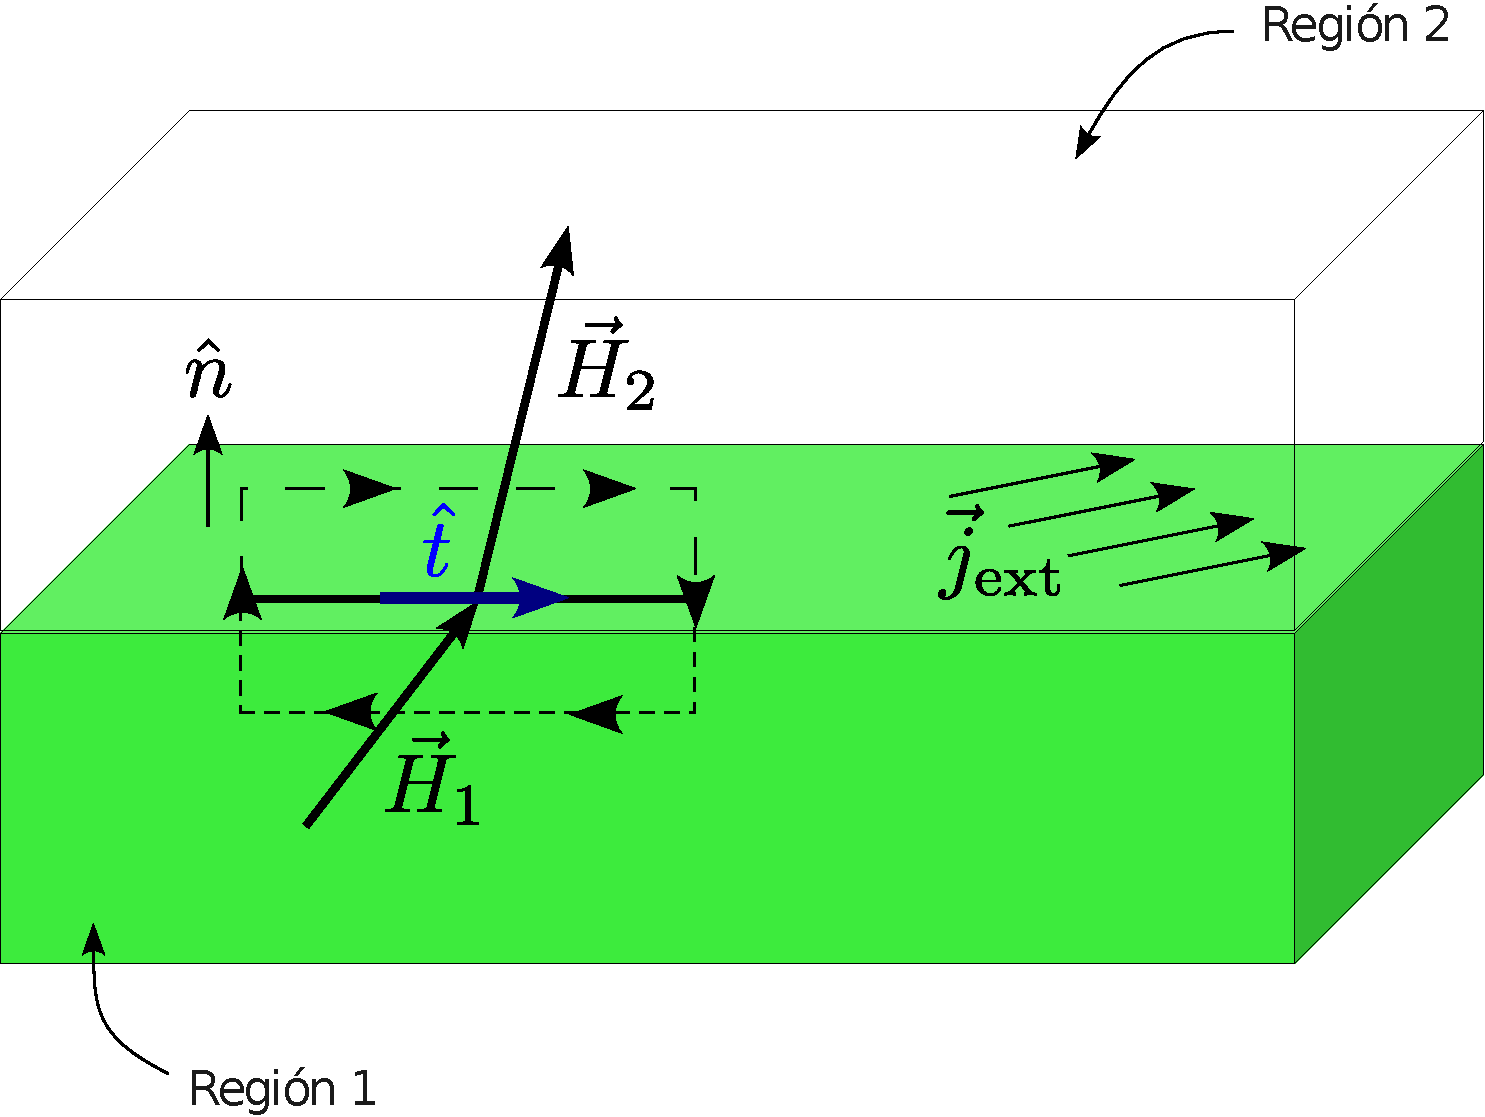
\psfig{file=fig/fig-condicion-borde-magnetica-01.pdf,height=5cm,angle=0}}
\caption{Condiciones de continuidad para $\vec{H}$ en una interface de dos
medios magn'eticos.}
\label{BM1}
\end{figure}
Al aplicar la ley de Amp\`ere (\ref{intHI}) al circuito de la figura \ref{BM1},
y considerando que
\begin{equation}\label{IextjS}
 I_{\rm ext}=\int_S\vec{J}_{\rm ext}\cdot d\vec{S}=\int_S\vec{J}_{\rm ext}\cdot
(\hat{n}\times\hat{t})\,dS=\vec{j}_{\rm ext}\cdot
(\hat{n}\times\hat{t})\,\ell=(\vec{j}_{\rm ext}\times\hat{n})\cdot\hat{t}\,\ell ,
\end{equation}
encontramos
\begin{equation}
 \boxed{\left(\vec{H}_2-\vec{H}_1\right)\cdot\hat{t}=(\vec{j}_{\rm
ext}\times\hat{n})\cdot\hat{t}} \label{Hint}
\end{equation}
o, equivalentemente
\begin{equation}
\boxed{\hat{n}\times\left(\vec{H}_2-\vec{H}_1\right)=\vec{j}_{\rm
ext}.}
\end{equation}
Note que en (\ref{IextjS}) el lado derecho contiene a la \textbf{densidad de corriente superficial externa} $\vec{j}_{\rm ext}$. En este caso puede considerarse que $\vec{J}_{\rm ext}=\vec{j}_{\rm ext}\delta(z)$, donde la superficie que limita las dos regiones est'a determinada por la condici'on $z=0$, siendo $z$ una coordenada normal a la superficie.

\textbf{Si no hay corrientes externas de superficie, entonces la componente \textit{tangencial} de la excitaci'on magn'etica cruza continuamente la interface}. En general, si
existen corrientes externas de superficie, la componente de la intensidad de
campo magn'etico paralela a $\vec{j}_{\rm ext}=j_{\rm ext}\,\hat{\jmath}$ cruzar'a continuamente la interface, mientras que la componente ortogonal tendr'a una discontinuidad de magnitud $j_{\rm ext}$. Esto puede verse directamente
de (\ref{Hint}) eligiendo $\hat{t}$ en la direcci'on y sentido de
$\vec{j}_{\rm ext}$, es decir, $\hat{t}=\hat{\jmath}$, obteniendo
\begin{equation}
 H_2^\parallel=H_1^\parallel,  \qquad H^\parallel:=\vec{H}\cdot\hat{\jmath},
\end{equation}
mientras que, eligiendo $\hat{t}=\hat{\jmath}\times\hat{n}$, encontramos
\begin{equation}
 H_2^\perp-H_1^\perp=j_{ext},  \qquad
H^\perp:=\vec{H}\cdot(\hat{\jmath}\times\hat{n}).
\end{equation}

Estas relaciones se complementan con aquella que se desprende del hecho que el campo magn'etico tiene siempre divergencia nula (independientemente del medio considerado). An'alogamente al caso el'ectrico, ver por ejemplo \eqref{saltoDn}, la ecuaci'on \eqref{divB} implica 
\begin{equation}\label{saltoBn}
\boxed{\left(\vec{B_2}-\vec{B_1}\right)\cdot\hat{n}=0,}
\end{equation}
es decir, la componente de $\vec{B}$ normal a la superficie es continua en la interface.

\subsection{Relaci'on constitutiva, susceptibilidad magn'etica}
An'alogamente al caso electrost'atico, se llama relaci'on constitutiva a la
relaci'on entre la magnetizaci'on de un material (la ``respuesta'' de 'este)
con el campo magn'etico existente, por ejemplo:
\begin{equation}
 \vec{M}=\vec{M}[\vec{H}].
\end{equation}
Esta relaci'on puede ser no-local, no-lineal, anis'otropa e inhomog'enea, y es usualmente inferida a partir de experimentos. Sin
embargo, muchos materiales pueden ser descritos por relaciones \textit{locales}. En
este caso puede parametrizarse la dependencia de la magnetizaci'on con la
intensidad magn'etica por medio de una serie de la forma
\begin{equation}
M_i(x)=M_i(H_j(x))=\left.M_i\right|_{\vec{H}=\vec{0}}
+\chi^{\rm m}_{ij}(x)H_j(x)+\chi^{\rm m}_{ijk}(x)H_j(x)H_k(x)+\cdots.
\end{equation}
%\begin{equation}
%M_i(x)=M_i(H_j(x))=\left.M_i\right|_{\vec{H}=\vec{0}}
%+H_j\left(\partial_jM_i\right)_{\vec{H}=\vec{0}}+\frac{1}{2}
%H_jH_k\left(\partial_j\partial_k M_i\right)_{\vec{H}=\vec{0}}+\cdots.
%\end{equation}
Para medios locales, \textit{lineales} y \textit{sin magnetizaci'on permanente}
($\left.M_i\right|_{\vec{H}=\vec{0}}=0$), la relaci'on se reduce a
\begin{equation}
 \boxed{M_i(x)=\chi^{\rm m}_{ij}(x)H_j(x),}
\end{equation}
donde $\chi^{\rm m}_{ij}$ es el \textbf{tensor de susceptibilidad magn'etica} del
material. En este caso, la inducci'on magn'etica adopta la forma
\begin{equation}
 \boxed{B_i(x)=\mu_{ij}(x)H_j(x)=\mu_0\,\kappa^{\rm m}_{ij}(x)H_j(x),}
\end{equation}
con el tensor de \textbf{permeabilidad magn'etica} $\mu_{ij}$ y el
tensor de \textbf{permeabilidad relativa} $\kappa^{\rm m}_{ij}$, definidos por
\begin{equation}
 \boxed{\mu_{ij}:=\mu_0\left(\delta_{ij}+\chi^{\rm
m}_{ij}\right)=\mu_0\kappa^{\rm m}_{ij}.}
\end{equation}
Finalmente, en el caso de medios locales, lineales e is'otropos, las
expresiones anteriores para la relaci'on constitutiva se reducen a
\begin{equation}
 \vec{M}(x)=\chi_{\rm m}(x)\vec{H}(x),
\end{equation}
\begin{equation}
 \vec{B}(x)=\mu(x)\vec{H}(x)=\mu_0\,\kappa_{\rm m}(x)\vec{H}(x),
\end{equation}
\begin{equation}
 \mu:=\mu_0\left(1+\chi_{\rm m}\right)=\mu_0\kappa_{\rm m}.
\end{equation}


\subsubsection{Ecuaci'on de Laplace para el potencial escalar de magnetizaci'on}
Como vimos en la secci'on \ref{sec:defH}, \textit{en regiones libres de corrientes externas} la excitaci'on magn'etica $\vec{H}$ es propocional al gradiente del potencial escalar de magnetizaci'on, ver (\ref{HpM}). Si adem'as el medio es \textit{lineal e is'otropo}, entonces $\vec{B}=\mu\vec{H}=-\mu\vec{\nabla}\phi^\ast_{\rm M}$. Finalmente, si adem'as el medio es \textit{homog'eneo}, encontramos, usando (\ref{divB}), que el potencial escalar de magnetizaci'on satisface la ecuaci'on de Laplace,
\begin{equation}
\nabla^2\phi^\ast_{\rm M}=0.
\end{equation}


\subsection{Paramagnetismo, diamagnetismo, ferromagnetismo}

\subsubsection{Diamagnetismo}
En este tipo de materiales $\vec{M}$ \textbf{tiene direcci'on opuesta a}  $\vec{H}$, por lo que $\chi_{\rm m}<0$ y $\kappa_{\rm m}<1$ y la inducci'on magn'etica $\vec{B}$ es \textbf{debilidata} (respecto al valor que asumir'ia en el vac'io, dada la misma distribuci'on de corrientes externas). Este tipo de materiales requiere que no existan \textit{momentos magn'eticos permanentes} significativos, de modo que la magnetizaci'on se deba principalmente a \textbf{corrientes inducidas}. Estas \textbf{corrientes inducidas generan momentos dipolares en sentido contrario al campo que las induce}, por lo que \textbf{la inducci'on magn'etica disminuye en el interior de un diamagneto}. En la mayor'ia de los casos de diamagnetismo la susceptibilidad magn'etica es independiente de la
temperatura y posee un valor muy peque\~no: $|\chi_{\rm m}|\lesssim 10^{-5}$. El
diamagnetismo es una propiedad general, es decir, que se presenta en todos los
materiales (siempre se producen peque\~nas corrientes inducidas), pero se dice
que un material es diamagn'etico si este efecto es el dominante, es decir,
cuando no existen otras fuentes de magnetizaci'on que reviertan la contribuci'on diamagn'etica.
Ejemplos de materiales diamagn'eticos: casi todas las substancias org'anicas,
metales nobles (oro, plata, cobre, mercurio, ...). Un caso extremo de
diamagnetismo es un \textbf{superconductor}, en el que la inducci'on magn'etica
es \textbf{anulada en su interior}, $\chi_{\rm m}=-1$ y $\kappa_{\rm m}=0$ (``diamagneto ideal'').

\subsubsection{Paramagnetismo}
 En este tipo de materiales la magnetizaci'on $\vec{M}$
tiene la misma direcci'on y sentido que $\vec{H}$. Equivalentemente $\vec{M}$
tiene la misma direcci'on y sentido que $\vec{B}$, de modo que
$\chi_{\rm m}>0$, $\kappa_{\rm m}>1$. Por esto, en un material paramagn'etico la inducci'on magn'etica $\vec{B}$ es \textbf{reforzada}. Este caso requiere que el material posea \textit{momentos magn'eticos permanentes}, que puedan anilearse con el campo magn'etico.
A la tendencia de los momentos magn'eticos a alinearse se
contrapone el ``desorden'' relacionado con las agitaciones t'ermicas del
material. Por esto, \textbf{en un material paramagn'etico $\chi_{\rm}$ disminuye a
medida que la temperatura aumenta}. Muchos materiales paramagn'eticos satisfacen
la \textbf{ley de Curie}: $\chi_{\rm}\propto 1/T$.
\begin{table}[h!]
\begin{center}
\begin{tabular}{c|c}
Material & $\chi_{\rm m}$ \\ \hline\hline
Aluminio & $2,1\times 10^{-5}$ \\
Cobre & $-0,98\times 10^{-5}$ \\
Oro & $-3,5\times 10^{-5}$ \\
Magnesio & $1.2\times 10^{-5}$ \\
Mercurio & $-2,8\times 10^{-5}$ \\
Plata & $-2,4\times 10^{-5}$ \\
Sodio & $0.84\times 10^{-5}$ \\
Titanio & $18.0\times 10^{-5}$ \\
Tungsteno & $7.6\times 10^{-5}$ \\
Hidr'ogeno (1 atm) & $-0,22\times 10^{-8}$ \\
Nitr'ogeno (1 atm) & $-0,67\times 10^{-8}$ \\
Ox'igeno (1 atm) & $193,5\times 10^{-8}$
\end{tabular}
\caption{Algunos materiales y sus susceptibilidades magn'eticas, a temperatura ambiente (Reitz-Milford).}
\end{center}
\end{table}

\subsubsection{Ferromagnetismo}

 En este tipo de materiales (t'ipicamente materiales que
contienen Fierro, Cobalto o N'iquel) \textbf{la magnetizaci'on no es
proporcional a la excitaci'on magn'etica}. Esto es algunas veces expresado
diciendo que la \textbf{susceptibilidad magn'etica efectiva} $\chi_{\rm m}:=M/H$ depende del valor del campo (y de otras variables, como por ejemplo de la temperatura), $\chi_{\rm m}=\chi_{\rm m}(T,\vec{H})$. El ferromagnetismo
requiere tambi'en que el material posea dipolos magn'eticos permanentes. Debido
a interacciones cu'anticas, los momentos magn'eticos de un ferromagneto se
ordenan \textit{espont'aneamente} (es decir, sin necesidad de campo magn'etico
externo), cuando la temperatura baja de un cierto valor cr'itico, llamada
temperatura de Curie, $T_{\rm C}$. En el cero absoluto de temperatura, todos los
momentos magn'eticos estar'ian alineados. A medida que la temperatura aumenta, el
desorden inducido por las vibraciones t'ermicas tiende a disminuir la
alineaci'on, pero sin conseguir
anular la magnetizaci'on total. Cuando la temperatura cruza la temperatura de
Curie, el sistema experimenta una transici'on de fase, y a partir de ese
momento se comporta como un paramagneto usual.
\begin{table}[h!]
\begin{center}
\begin{tabular}{c||c|c|c|c|c|c}
Material & Fe & Co & Ni & Gd & EuO & CrBr${}_3$  \\ \hline
$T_{\rm C}$ [K] & 1043 & 1393 & 631 & 290 & 69 & 37
\end{tabular}
\caption{Algunos materiales ferromagn'eticos y sus temperaturas de Curie 
\cite{Nolting}.}
\end{center}
\end{table}

T'ipicamente, los ferromagnetos poseen susceptibilidades
magn'eticas muy altas y \textbf{la magnetizaci'on que presentan depende de
su historia}, es decir, de c'omo hayan sido expuestos a campos externos. En
otras palabras, \textbf{dado un valor de la excitaci'on $\vec{H}$ el valor de $\vec{M}$
no es 'unico, sino que depende de c'omo se haya alcanzado el valor $\vec{H}$}.
Este fen'omeno es conocido como \textbf{hist'eresis}. El comportamiento de
hist'eresis t'ipico de un ferromagneto es ilustrado en la figura
\ref{fig-histeresis}.
\begin{figure}[!h]
\centerline{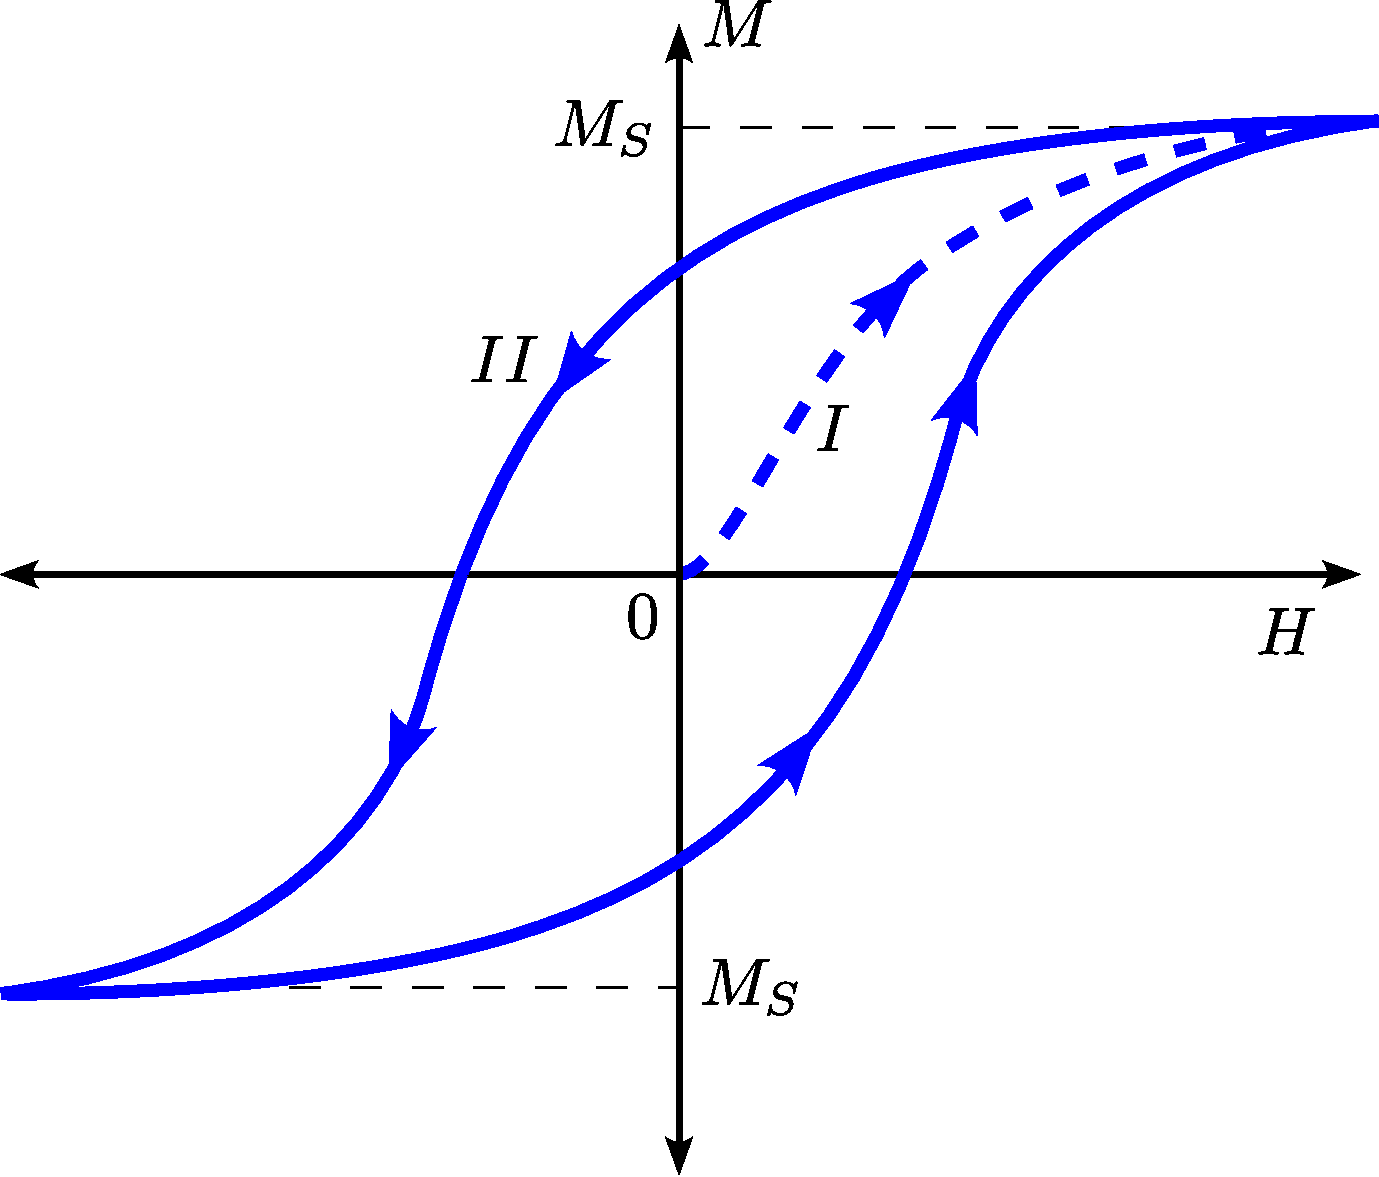
\psfig{file=fig/fig-histeresis-01.pdf,height=6cm,angle=0}}
\caption{Curva de hist'eresis t'ipica para un material ferromagn'etico.}
\label{fig-histeresis}
\end{figure}
Un material ferromagn'etico sin magnetizaci'on previa sometido a un campo $H$
se magnetiza siguiendo la curva I, llegando a una magnetizaci'on m'axima $M_S$ (``magnetizaci'on de saturaci'on"). 
Si luego se disminuye la intensidad de campo magn'etico el sistema se comienza
a demagnetizar, pero siguiendo la curva II, de modo que, incluso cuando el
campo $H$ es cero, el material conserva una magnetizaci'on no nula (magneto
permanente), llamada ``magnetizaci'on remanente''. Esta magnetizaci'on puede
ser anulada aplicando un campo en sentido inverso (intensidad de campo
``coercitivo''). La propiedad de hist'eresis est'a relacionada con la existencia
de \textbf{dominios magn'eticos}, que poseen un momento magn'etico macrosc'opico
no nulo y que requieren de energ'ia para reorientarse. La hist'eresis de los
ferromagnetos es usada en la fabricaci'on de \textbf{dispositivos de memoria}, en los
que la informaci'on es codificada en la orientaci'on del momento magn'etico de
los dominios, que permanece indefinidamente hasta que campos externos sean
usados para cambiar su estado.
\newpage
\chapter{Electrodin'amica}

\section{Ley de inducci'on de Faraday}

Faraday\footnote{Michael Faraday (1791-1867): f'isico y qu'imico brit'anico. Ver \url{http://es.wikipedia.org/wiki/Michael_Faraday}.} encontr'o experimentalmente (1831) que \textit{si el flujo magn'etico a trav'es de una espira cerrada var'ia en el tiempo, se induce una corriente sobre una espira}. Si el flujo es constante, se observa que la corriente desaparece. La \textbf{ley de Faraday} se escribe como
\begin{equation}\label{faraday}
\varepsilon_{\rm ind}=-K\frac{d\phi}{dt},
\end{equation}
donde $\varepsilon_{\rm ind}$ es la fuerza electromotriz (f.e.m.) \textit{inducida} en la espira. El signo menos describe la direcci'on de la corriente inducida, dada por la \textbf{ley de Lenz}. Aqu'i $K$ es una constante que depende del sistema de unidades usado. En el Sistema Internacional es una cantidad adimensional, que determinaremos m'as adelante.

En t'erminos de campos, se genera un campo el'ectrico $\vec{E}$ que es el que hace mover las cargas en la espira, es decir,
\begin{equation}
\oint_{\cal\partial S}\vec{E}\cdot d\vec{\ell}=\varepsilon_{\rm ind}.
\end{equation}
Con esto, podemos escribir (\ref{faraday}) como
\begin{equation}
\oint_{\cal \partial S}\vec{E}\cdot d\vec{\ell}=-K\frac{d\ }{dt}\int_S\vec{B}\cdot
d\vec{S}.
\end{equation}
En general, la superficie puede variar en el tiempo. Si 'este \textit{no} es el caso, y $S$
es constante, entonces podemos deducir que
\begin{equation}\label{ley-faraday0}
\vec\nabla\times\vec{E}=-K\frac{\partial\vec{B}}{\partial t}.
\end{equation}
Considere ahora el caso en que la espira se mueve \textit{r'igidamente}, es decir, que la velocidad de los puntos de la espira es independiente de la posici'on (puede, sin embargo, depender del tiempo).
Entonces el cambio del flujo por la superficie, entre los tiempos $t$ y $t+dt$, puede calcularse como sigue:
\begin{eqnarray}
 d\Phi &=& \Phi(t+dt)-\Phi(t)\\
&=&
\int_{S(t+dt)}B_i(\vec{x}+\vec{v}dt,t+dt)dS_i-\int_{S(t)}B_i(\vec{x},t)dS_i\\
&=&\int_{S(t+dt)}\left[B_i(\vec{x},t)+dt\,v_j\,\partial_jB_i(\vec{x},
t)+dt\,\partial_tB_i(\vec{x},t)\right ] dS_i-\int_{S(t)}B_i(\vec{x},t)dS_i\\
&=&\int_S\left[B_i(\vec{x},t)+dt\,v_j\,\partial_jB_i(\vec{x},
t)+dt\,\partial_tB_i(\vec{x},t)\right ] dS_i-\int_SB_i(\vec{x},t)dS_i\\
&=&dt\int_S\left[v_j\,\partial_jB_i(\vec{x},t)+\partial_tB_i(\vec{x},t)\right
] dS_i.
\end{eqnarray}
En la pen'ultima igualdad usamos el hecho que el elemento de superficie $dS_i$ sobre la superficie $S(t)$ y $S(t+dt)$ son iguales, ya que la superficie se mueve r'igidamente (es decir, con igual velocidad en cada punto). As'i obtenemos que
\begin{equation}\label{dPhidt0}
 \frac{d\Phi}{dt}=\int_S\left[v_j\,\partial_jB_i(\vec{x},t)+\partial_tB_i(\vec
{x},t)\right] dS_i.
\end{equation}
Usamos ahora la identidad
\begin{equation}
\varepsilon_{ijk}\partial_j(\varepsilon_{klm}B_lv_m)\equiv
v_j(\partial_jB_i)-v_i(\partial_jB_j),
\end{equation}
y la ley (\ref{divB}) (que suponemos v'alida incluso en el caso din'amico) para reescribir (\ref{dPhidt0}) como
\begin{eqnarray}
 \frac{d\Phi}{dt}&=&\int_S\left[\partial_tB_i+\varepsilon_{ijk}
\partial_j(\varepsilon_{klm} B_lv_k)\right] dS_i \\
&=& \int_S\partial_tB_i\, dS_i +\oint_{\partial S}\varepsilon_{ijk}
B_jv_k\,dx_i 
\end{eqnarray}
o, en notaci'on vectorial, 
\begin{equation}\label{dFlujodt}
  \frac{d\Phi}{dt}=\int_S\frac{\partial\vec{B}}{\partial
t}\cdot d\vec{S}-\oint_{\partial
S}\left(\vec{v}\times\vec{B}\right)\cdot d\vec{\ell}.
\end{equation}
Apliquemos estos resultados para comparar la descripci'on, respecto a dos sistemas de referencia inerciales (SRI's), del fen'omeno de inducci'on de corriente en una espira debido a la variaci'on de flujo magn'etico. Primero, en el SRI $K$ en el que la espira est'a en reposo y el magneto se mueve tenemos que en cada punto del espacio el campo magn'etico $\vec{B}$ depender'a del tiempo, por lo que se inducir'a un campo el'ectrico de acuerdo a (\ref{ley-faraday0}). Este campo el'ectrico ejercer'a una fuerza $\vec{F}_q=q\vec{E}$ sobre una carga $q$ en la espira, que consideraremos inicialmente en reposo. 

Por otro lado, en un SRI $K'$ con velocidad relativa $\vec{v}$ respecto a $K$ (de modo que en $K'$ el magneto est'a en reposo) la corriente inducida es debido al movimiento de la espira. Si en este SRI el campo magn'etico es $\vec{B}'(x)$, no existe campo el'ectrico inducido puesto que $\partial\vec{B}'/\partial t=\vec{0}$. En este SRI la corriente inducida se describe 'integramente debido a la fuerza de Lorentz ejercida por el campo magn'etico sobre las cargas en la espira, que ahora se mueven con velocidad $-\vec{v}$. La fuerza que act'ua sobre la carga es ahora $\vec{F}'_q=-q\vec{v}\times\vec{B'}$. Adem'as, la f.e.m. est'a dada, usando el resultado (\ref{dFlujodt}) aplicado a este caso, as'i como la ley de Faraday (\ref{ley-faraday0}), por 
\begin{equation}
\varepsilon'_{\rm ind}=-K\oint_{\partial S}\left(\vec{v}\times\vec{B}'\right)\cdot d\vec{\ell}.
\end{equation}

 Ya que $K$ y $K'$ son SRI's, la aceleraci'on, y por tanto la fuerza que act'ua sobre la carga (inicialmente en reposo en $K$), son necesariamente iguales. De lo anterior, es decir $\vec{F}_q=\vec{F}'_q$, vemos que esto s'olo es posible si el campo inducido es dado por
 \begin{equation}\label{EvBp}
\vec{E}=-\vec{v}\times\vec{B'}.
\end{equation}
Adem'as, la f.e.m. debe ser la misma, ya que la corriente inducida lo es, por lo que
\begin{align}
\varepsilon_{\rm ind} &= \varepsilon'_{\rm ind}, \\
\oint_{\partial S}\vec{E}\cdot d\vec{\ell} &=-K\oint_{\partial S}\left(\vec{v}\times\vec{B}'\right)\cdot d\vec{\ell}.
\end{align}
Usando ahora (\ref{EvBp}) en el lado izquierdo obtenemos
\begin{equation}
-\oint_{\partial S}\left(\vec{v}\times\vec{B'}\right)\cdot d\vec{\ell} =-K\oint_{\partial S}\left(\vec{v}\times\vec{B}'\right)\cdot d\vec{\ell}.
\end{equation}
Esta relaci'on implica que la constante $K$ debe tener, en el Sistema Internacional de Unidades, el valor $K=1$. 

De esta forma, la ley de Faraday adopta la forma
\begin{equation}
\boxed{\oint_{\cal\partial S}\vec{E}\cdot d\vec{\ell}=-\frac{d\ }{dt}\int_S\vec{B}\cdot
d\vec{S}}
\end{equation}
o, en forma diferencial:
\begin{equation}
\boxed{\vec\nabla\times\vec{E}=-\frac{\partial\vec{B}}{\partial t}.}
\label{ley-faraday}
\end{equation}

%\subsection{Autoinducci'on}
%\begin{equation}
% L:=\frac{d\Phi}{dI}
%\end{equation}
%\begin{equation}
% \varepsilon_{\rm ind}=-L\frac{dI}{dt}
%\end{equation}


\subsection{Energ'ia del campo magn'etico}

Consideremos ahora una espira por la que circula una corriente $I$ y el campo magn'etico \textit{que ella misma produce}. Si $I$ no var'ia en el tiempo, no existe fem inducida ya que el flujo magn'etico por la espira permanece constante (suponemos una espira fija, en reposo). Calcularemos la energ'ia necesaria para cambiar la corriente $I$ y el correspondiente campo magn'etico $\vec{B}$ en una peque\~na cantidad. Durante el intervalo de tiempo $dt$ en que la corriente cambia en $dI$ y el campo magn'etico en $d\vec{B}$, se genera un campo el'ectrico inducido y su correspondiente fem $\varepsilon$ (que en general se superponen al campo y fem que mantien'ian la corriente $I$ fluyendo originalmente). Este campo inducido ``intenta reducir'' el cambio de la corriente. Para esto, el campo realiza trabajo sobre las cargas en movimiento en la espira. 
%Calcularemos la energ'ia transferida a las cargas que se ponen en movimiento para formar la corriente inducida en una espira, debido a la inducci'on de Faraday. Para esto, consideraremos una espira que forma una curva cerrada $\cal C$ por la que circula una corriente inducida $I$. 

Dividiremos la curva en elementos de longitud $d\vec{\ell}=d\ell \,\hat{t}$, en los que existe una carga $dq=\lambda d\ell$. El vector unitario $\hat{t}$ est'a definido de modo que $d\vec{\ell}$ tiene la orientaci'on standard respecto al vector normal $\hat{n}$ a la superficie que encierra la espira. El campo el'ectrico $\vec{E}$ ejerce trabajo sobre las cargas $dq$. En un intervalo de tiempo $dt$ el trabajo realizado sobre las cargas $dq$ es entonces 
\begin{align}
dq\,\vec{E}\cdot d\vec{\ell} &= (\lambda d\ell) \vec{E}\cdot (\vec{v}\,dt) \\
&= (\lambda d\ell) \vec{E}\cdot (v\,\hat{t})\,dt \\
&= (\lambda v) \vec{E}\cdot (d\ell\,\hat{t})\,dt \\
&= I(\vec{E}\cdot d\vec{\ell})\,dt.
\end{align}
Aqu'i hemos identificado la corriente $I=\lambda v$ sobre la espira, y tomado en cuenta que $\vec{v}=v\hat{t}$. Por lo tanto, el trabajo total realizado por el campo sobre las cargas de la espira, en el intervalo de tiempo $dt$, es dado por
\begin{align}
dW &= \oint_{\cal C}dq\,\vec{E}\cdot d\vec{\ell} \\
&= I\oint_{\cal C}(\vec{E}\cdot d\vec{\ell})\,dt \\
&= I\varepsilon\,dt \\
&= -I\frac{d\Phi}{dt}\,dt \\
&= -I\,d\Phi.
\end{align}

A partir de este resultado vemos que la energ'ia (proveniente de fuentes externas) necesaria para cambiar el flujo magn'etico en una cantidad $d\Phi$, en un sistema con una corriente $I$ es dada por
\begin{equation}\label{dWIdP}
 \boxed{dU=I\,d\Phi.}
\end{equation}
En otras palabras, \textit{un cambio en el valor de la intensidad de campo $\vec{B}$ requiere invertir energ'ia}. En cierto sentido, la ley de Faraday establece una cierta ``inercia'' en el campo magn'etico, ya que un sistema de cargas y campos tiende a ``resistirse'' al cambio del valor del campo (y su flujo). 
Esto implica adem'as que \textit{es necesario asociar una energ'ia a una cierta configuraci'on de campos y corrientes}, puesto que es necesario invertir energ'ia para establecer estas corrientes y sus campos asociados. Para evaluar esta energ'ia, reescribiremos (\ref{dWIdP}) usando (\ref{PAdx}): la energ'ia $\delta U$ necesaria para variar el potencial vectorial $\vec{A}(x)$ de un sistema de corrientes y campo magn'etico en $\delta\vec{A}(x)$ es dada por
\begin{align}
 \delta U &= I\oint_{\cal C}\delta\vec{A}\cdot d\vec{\ell} \\
 &= \oint_{\cal C}\delta\vec{A}\cdot Id\vec{\ell} \\
 &= \int_V\delta\vec{A}\cdot \vec{J}_{\rm ext}\,dV. \label{WdAJ}
\end{align}
En el 'ultimo paso hemos usado la relaci'on (\ref{IdxJdV}) para reescribir la energ'ia en t'erminos de una integral de volumen de la densidad de corriente. Note que la corriente inducida es en general corriente ``externa'' o de ``conducci'on'', por lo que hemos explicitado en el 'ultimo t'ermino la densidad de corrientes externas $\vec{J}_{\rm ext}$. Adem'as, usando la ley de Amp\`ere para la excitaci'on magn'etica (\ref{rotHj}), podemos escribir
\begin{align}
 \delta U 
&= \int_{V'} \delta A_i\,\varepsilon_{ijk}\left(\partial_jH_k\right)\,dV \\
&= \varepsilon_{ijk}\int_{V'} \left[\partial_j(H_k\delta A_i)-H_k(\partial_j\delta A_i)\right]dV\\
&= \varepsilon_{ijk}\oint_{\partial V'}H_k\delta
A_i\,dS_j-\varepsilon_{ijk}\int_{V'}H_k(\partial_j\delta A_i)\,dV\\
&= 0+\int_{V'} H_k\,\varepsilon_{kji}(\partial_j\delta A_i)\,dV\\
&= \int_{V'} H_k\,\delta B_k\,dV.
\end{align}
Aqu'i hemos extendido el dominio de integraci'on a un volumen $V'\to R_3$, es decir, a todo el espacio, usado el teorema de Gauss y considerado que la integral de superficie se anula en el infinito. Con esto, obtenemos la siguiente expresi'on para la \textit{energ'ia requerida para cambiar la inducci'on magn'etica de un sistema en $\delta{\vec B}(x)$}:
\begin{equation}
 \boxed{\delta U=\int_{R^3} \vec{H}(x)\cdot \delta\vec{B}(x)\,dV.}\label{dUB}
\end{equation}
Note la similitud entre las expresiones (\ref{WdAJ}) y (\ref{dUB}) con los resultados (\ref{Wdiel1}) y (\ref{dUE}) para la energ'ia almacenada por un campo el'ectrico, respectivamente.

*** Agregar comentario energ'ia y 'area bajo la curva de gr'afico $H$ v/s $B$ ***

Similarmente a lo discutido en el caso el'ectrico, la \textit{energ'ia total requerida para aumentar el campo magn'etico de un sistema desde cero hasta un valor final $\vec{B}$} es 
\begin{equation}
 U=\int_0^1\int_{R^3} \lambda \, \vec{H}(x)\cdot \delta\vec{B}_\lambda(x)\,dV,
\end{equation}
donde $\vec{B}_\lambda(x)$ es el valor de la inducci'on magn'etica correspondiente al caso en que la excitaci'on magn'etica tiene un valor $\vec{H}_\lambda(x)$ igual a una fracci'on $\lambda$ de la excitaci'on magn'etica final, es decir, $\vec{H}_\lambda (x)=\lambda\vec{H}_\lambda (x)$ .

En el caso de un \textit{medio magn'etico lineal}, tendremos que $\vec{B}_\lambda (x)=\lambda\, \vec{B}(x)$ y por lo tanto $\delta\vec{B}_\lambda (x)=d\lambda\,
\vec{B}(x)$, y entonces
\begin{equation}\label{UHB}
 \boxed{U=\frac{1}{2}\int_{R^3} \vec{H}(x)\cdot\vec{B}(x)\,dV }
\end{equation}
o, alternativamente, 
\begin{equation}
 \boxed{U=\frac{1}{2}\int_{R^3} \vec{A}\cdot \vec{J}\,dV.}
\end{equation}

Usando (\ref{UHB}) podemos escribir la energ'ia almacenada en un sistema de campo magn'etico (y corrientes) como la integral de una \textbf{densidad de energ'ia magn'etica}
\begin{equation}
 \boxed{U=\int_{R^3} u_B(x)\,dV, \qquad u_B(x):=\frac{1}{2}\vec{H}(x)\cdot\vec{B}(x).}
\end{equation}
En el caso particular de medio lineales e is'otropos la densidad de energ'ia magn'etica se reduce a
\begin{equation}
 u_B(x)=\frac{\mu}{2}\vec{H}^2(x)=\frac{1}{2\mu}\vec{B}^2(x).
\end{equation}


\subsection{Fuerzas y torques sobre circuitos magn'eticos}
%\begin{equation}
%\boxed{F_i=-\left(\frac{\partial U}{\partial x_i}\right) ,} \label{FQB}
%\end{equation}
%
%\begin{equation}
% \boxed{\vec{\tau}\cdot\hat{n}=-\left(\frac{\partial U}{\partial\theta}\right).}
%\end{equation}

\section{Ecuaciones de Maxwell}
Hasta el momento,
\begin{align}
\vec\nabla\cdot\vec{D} & =\rho ,\label{cmax1}\\
\vec\nabla\cdot\vec{B}  & =0 ,\label{cmax2}\\
\vec\nabla\times\vec{H}  & =\vec{J} ,\label{cmax3}\\
\vec\nabla\times\vec{E}  & =-\frac{\partial\vec{B}}{\partial t} .\label{cmax4}
\end{align}
Note que aqu'i hemos suprimido, para no recargar la notaci'on, la designaci'on ``${\rm ext}$'' en la densidad de carga y corriente externa.

Vemos que (\ref{cmax3}) implica $\vec\nabla\cdot\vec{J}=0$, que es una condici'on que \textit{no es v'alida en general}, sino que s'olo en los casos, de acuerdo a (\ref{eccont}), en que ${\partial\rho}/{\partial t}=0$. Esto lleva a pensar que (al menos) la ecuaci'on (\ref{cmax3}) no es v'alida en el caso din'amico m'as general en el que las densidades de carga y corriente, y por lo tanto los campos el'ectricos y magn'eticos, var'ian en el tiempo.

Maxwell\footnote{James Clerk Maxwell (1831-1879): F'isico escoc'es. Ver \url{http://es.wikipedia.org/wiki/James_Clerk_Maxwell}.} (1861) generaliz'o la ecuaci'on (\ref{cmax3}) de modo que sea compatible con (\ref{cmax1}) y la ley de conservaci'on de la carga el'ectrica,
es decir, con la ecuaci'on de continuidad (\ref{eccont}). Usando (\ref{cmax1}), que suponemos por tanto v'alida en el caso general, podemos escribir (\ref{eccont}) como
\begin{eqnarray}
 0&=&\frac{\partial\rho}{\partial t}+\vec{\nabla}\cdot\vec{J}\\
&=& \frac{\partial\ }{\partial
t}\left(\vec\nabla\cdot\vec{D}\right)+\vec{\nabla}\cdot\vec{J}\\
&=& \vec\nabla\cdot\left[\frac{\partial\vec{D}}{\partial t}
+\vec{J}\right].
\end{eqnarray}
De aqu'i vemos que en el caso de corrientes generales (no-est'aticas), $\vec{J}$ tiene divergencia no nula, pero la combinaci'on $\vec{J}+{\partial\vec{D}}/{\partial t}$ \textit{siempre tiene divergencia nula}. A partir de esta observaci'on, Maxwell \textit{postul'o} que el lado derecho de la ecuaci'on (\ref{cmax3}) deb'ia ser reemplazada por la combinaci'on $\vec{J}+{\partial\vec{D}}/{\partial t}$. En otras palabras, Maxwell postul'o que a la densidad de corriente deber'ia agregarse el t'ermino ${\partial\vec{D}}/{\partial t}$, llamado \textit{corriente de desplazamiento}.

Con esto, las ecuaciones de Maxwell adoptan la forma:
\begin{align}
\vec\nabla\cdot\vec{D} & =\rho ,\label{max1}\\
\vec\nabla\cdot\vec{B}  & =0 ,\label{max2}\\
\vec\nabla\times\vec{H}  & =\vec{J}+\frac{\partial\vec{D}}{\partial
t} ,\label{max3}\\
\vec\nabla\times\vec{E}  & =-\frac{\partial\vec{B}}{\partial t}.\label{max4}%
\end{align}

Estas ecuaciones son completadas con las relaciones constitutivas entre
$\vec{E}$ y $\vec{D}$, y entre $\vec{B}$ y $\vec{H}$, as'i como con la expresi'on de la (densidad de) fuerza de Lorentz:
\begin{equation}
\vec{f}=\rho\vec{E}+\vec{J}\times\vec{B}.
\end{equation}

\section{Conservaci'on de la energ'ia y Vector de Poynting}\label{sec:energia}
Calculamos el producto escalar de $\vec{E}$ con la ecuaci'on (\ref{max3}).
Usando notaci'on tensorial, obtenemos:
\begin{equation}
 E_i\frac{\partial D_i}{\partial t}
-E_i\,\varepsilon_{ijk}\partial_jH_k+E_iJ_i=0.
\end{equation}
An'alogamente, el producto escalar entre $\vec{H}$ con la ecuaci'on
(\ref{max4}) implica,
\begin{equation}
H_i\frac{\partial B_i}{\partial t} +H_i\varepsilon_{ijk}\partial_jE_k=0.
\end{equation}
Sumando estas ecuaciones, obtenemos
\begin{align}
0 &= E_i\frac{\partial D_i}{\partial t}+H_i\frac{\partial B_i}{\partial t}
-E_i\varepsilon_{ijk}\partial_jH_k+E_iJ_i+H_i\varepsilon
_{ijk}\partial_jE_k\\
 &= E_i\frac{\partial D_i}{\partial t}+H_i\frac{\partial B_i}{\partial
t}+E_iJ_i+\varepsilon_{ijk}\left(H_i\partial_jE_k-E_i\partial_jH_k\right)\\
 &= E_i\frac{\partial D_i}{\partial t}+H_i\frac{\partial B_i}{\partial
t}+E_iJ_i+\varepsilon_{ijk}\left(H_i\partial_jE_k+E_k\partial_jH_i\right)\\
 &= E_i\frac{\partial D_i}{\partial t}+H_i\frac{\partial B_i}{\partial
t}+E_iJ_i+\partial_j(\varepsilon_{jki}E_kH_i).
\end{align}
En resumen, las ecuaciones de Maxwell (\ref{max3}) y (\ref{max4}) implican que
\begin{equation}
\boxed{\vec{E}\cdot\frac{\partial \vec{D}}{\partial
t}+\vec{H}\cdot\frac{\partial\vec{B}}{\partial t}+
\vec\nabla\cdot(\vec{E}\times\vec{H})
+\vec{E}\cdot\vec{J}=0.} \label{cEem0}
\end{equation}
Es 'util definir el \textit{vector de Poynting}\footnote{John Henry Poynting (1852-1914): f'isico ingl'es. Ver \url{http://es.wikipedia.org/wiki/John_Henry_Poynting} $\leftarrow$ \textbf{Esta p'agina podr'ia ser mejorada considerablemente, traduciendo la correspondiente en ingl'es!. ?`voluntarios?}} como
\begin{equation}\label{defPoy}\marginnote{Vector de Poynting}
\boxed{\vec{S}:=\vec{E}\times\vec{H}.}
\end{equation}
En un peque\~no intervalo de tiempo $dt$ los campos cambian (en cada punto fijo del espacio) en las peque\~nas cantidades dadas por $d\vec{D}=dt\,({\partial \vec{D}}/{\partial t})$ y
$d\vec{B}=dt\,({\partial \vec{B}}/{\partial t})$. Entonces podemos escribir
\begin{equation}
\vec{E}\cdot
d\vec{D}+\vec{H}\cdot d\vec{B}+\vec\nabla\cdot\vec{S}\,dt+\vec{E}\cdot\vec{J}\,
dt=0,
\end{equation}
que, integrado en un volumen $V$ conduce a 
\begin{equation}
\boxed{\int_V\left[\vec{E}\cdot d\vec{D}+\vec{H}\cdot
d\vec{B}\right]dV+\oint_{\partial V}
\vec{S}\cdot d\vec{S}\,dt+\int_V\vec{E}\cdot\vec{J}\,
dVdt=0.} \label{cEem1}
\end{equation}
Identificamos el 'ultimo t'ermino como el \textbf{trabajo realizado por el campo el'ectrico sobre las corrientes}, es decir, la energ'ia transferida del campo a las cargas (o viceversa, dependiendo del signo). Adem'as, de acuerdo a los resultados previos (\ref{dUE}) y (\ref{dUB}) la primera integral puede interpretarse como el \textbf{cambio total de la energ'ia almacenada en forma de campo el'ectrico y magn'etico}, en el volumen $V$. Finalmente, interpretamos la integral de superficie como la \textbf{energ'ia electromagn'etica neta que fluye a trav'es de la superficie $\partial V$}. En otras palabras, interpretamos el vector de Poynting como la \textit{densidad de flujo de energ'ia} electromagn'etica (la energ'ia electromagn'etica transportada por unidad de superficie y unidad de tiempo). De esta forma, (\ref{cEem1}) es una \textit{ecuaci'on de balance (o conservaci'on) de la energ'ia}.

En el caso particular de \textit{medios lineales, no disipativos, y con susceptibilidades
independientes del tiempo}, es decir, tales que
\begin{equation}
D_i=\varepsilon_{ij}E_j, \qquad \partial_t\varepsilon_{ij}=0, \qquad \varepsilon_{ij}=\varepsilon_{ji},
\end{equation}
\begin{equation}
B_i=\mu_{ij}H_j, \qquad \partial_t\mu_{ij}=0, \qquad \mu_{ij}=\mu_{ji},
\end{equation}
podemos reescribir:
\begin{equation}
 \vec{E}\cdot\frac{\partial \vec{D}}{\partial
t}=\frac{1}{2}\frac{\partial\ }{\partial t}\left(\vec{E}\cdot\vec{D}\right),
\qquad
 \vec{H}\cdot\frac{\partial \vec{B}}{\partial
t}=\frac{1}{2}\frac{\partial\ }{\partial t}\left(\vec{H}\cdot\vec{B}\right).
\end{equation}
Con esto, (\ref{cEem0}) es equivalente a
\begin{equation}
\boxed{\frac{\partial u}{\partial
t}+\vec\nabla\cdot\vec{S}+\vec{E}\cdot\vec{J}=0 ,} \label{econtEem}
\end{equation}
donde hemos definido la \textit{densidad de energ'ia del campo
electromagn'etico}:
\begin{equation}\label{uDEHB}
\boxed{u:=\frac{1}{2}\left(\vec{D}\cdot\vec{E}+\vec{H}\cdot\vec{B}\right).}
\end{equation}
La versi'on integral de (\ref{econtEem}) es
\begin{equation}
\frac{d\ }{dt}\left(E_{\rm em}+E_{\rm mec}\right)+\oint_{\partial
V}\vec{S}\cdot d\vec{S}=0 ,
\end{equation}
donde
\begin{equation}
E_{\rm em}=\int_V u\,dV
\end{equation}
es la \textbf{energ'ia electromagn'etica} y, de acuerdo al \textit{teorema de trabajo-energ'ia} \textit{en el caso que no existan otras fuerzas que realicen trabajo sobre las cargas},
\begin{equation}
 \frac{dE_{\rm mec}}{dt}=\int_V\vec{E}\cdot\vec{J}\,dV
\end{equation}
es la variaci'on de energ'ia mec'anica total de las cargas contenidas en $V$.

\section{Conservaci'on del momentum lineal}\label{sec:momentum}
La \textbf{fuerza total que el campo electromagn'etico ejerce sobre las cargas} contenidas en un volumen $V$ es dada por la fuerza de Lorentz:
\begin{equation}
\vec{F}_{\rm em}=\int_V\left(\rho\vec{E}+\vec{J}\times\vec{B}\right)dV .
\end{equation}
Consideremos el integrando de la expresi'on anterior (es decir, la densidad de fuerza) y reemplacemos las fuentes $\rho$ y $\vec{J}$ usando las ecuaciones de Maxwell inhomog'eneas (\ref{max1}) y (\ref{max3}). Con esto, tenemos que
\begin{eqnarray}
f_i&=&\rho E_i+\varepsilon_{ijk}J_jB_k \\
&=&(\partial_jD_j)E_i+\varepsilon_{ijk}(\varepsilon_{
jlm}\partial_lH_m-\partial_tD_j)B_k  \\
&=& \partial_j(D_jE_i)-D_j\partial_jE_i +
(\partial_kH_i)B_k-(\partial_iH_k)B_k-\varepsilon_{ijk}(\partial_tD_j)B_k \\
&=& \partial_j(D_jE_i)-D_j\partial_jE_i +
\partial_k(H_iB_k)-H_i(\partial_kB_k) \nonumber\\
&& -\partial_i(H_kB_k)+H_k(\partial_iB_k)
-\partial_t(\varepsilon_{ijk} D_jB_k)
+\varepsilon_{ijk} D_j(\partial_tB_k) \\
%&=&\partial_j(E_iD_j+H_iB_j-\delta_{ij}H_kB_k)
%-D_j\partial_jE_i+H_j(\partial_iB_j) \nonumber\\
%&& -\partial_t(\varepsilon_{ijk} D_jB_k)
%+\varepsilon_{ijk} D_j(\partial_tB_k) \\
&=&\partial_j(E_iD_j+H_iB_j-\delta_{ij}H_kB_k)
-D_j\partial_jE_i+H_j(\partial_iB_j) \nonumber\\
&& -\partial_t(\varepsilon_{ijk}
D_jB_k)-\varepsilon_{ijk} D_j(\varepsilon_{klm}\partial_lE_m) \\
&=&\partial_j(E_iD_j+H_iB_j-\delta_{ij}H_kB_k)
-D_j\partial_jE_i+H_j(\partial_iB_j) \nonumber\\
&& -\partial_t(\varepsilon_{ijk} D_jB_k)-D_j(\partial_iE_j) +D_j(\partial_jE_i)\\
&=&\partial_j(E_iD_j+H_iB_j-\delta_{ij}H_kB_k)-\partial_t(\varepsilon_{ijk}
D_jB_k)+H_j(\partial_iB_j)- D_j(\partial_iE_j). \label{flc}
\end{eqnarray}
En el caso de medios \textit{lineales, homog'eneos y no disipativos}, es decir, para medios tales que
\begin{equation}
 D_i=\varepsilon_{ij}E_j, \qquad \partial_k\varepsilon_{ij}=0, \qquad \varepsilon_{ij}=\varepsilon_{ji},
\end{equation}
\begin{equation}
 B_i=\mu_{ij}H_j, \qquad \partial_k\mu_{ij}=0,\qquad \mu_{ij}=\mu_{ji},
\end{equation}
podemos escribir
\begin{equation}
 \partial_i(D_jE_j)=\varepsilon_{jk}\partial_i(E_kE_j)=2\varepsilon_{jk}
E_k(\partial_i E_j)=2D_j(\partial_i E_j),
\end{equation}
es decir,
\begin{equation}
 D_j(\partial_i E_j)=\frac{1}{2}\partial_i(D_jE_j). \label{idl1}
\end{equation}
An'alogamente,
\begin{equation}
 H_j(\partial_i B_j)=\frac{1}{2}\partial_i(H_jB_j). \label{idl2}
\end{equation}
Reemplazando (\ref{idl1}) y (\ref{idl2}) en los 'ultimos dos t'erminos de
(\ref{flc}), encontramos
\begin{equation}
 \rho E_i+\varepsilon_{ijk}J_jB_k
=\partial_j\left[E_iD_j+H_iB_j-\frac{1}{2}\delta_{ij}\left(
E_kD_k+H_kB_k\right)\right]-\partial_t(\varepsilon_{ijk}D_jB_k).
\end{equation}
Definimos la \textbf{densidad de momentum} del campo, $\pi_i$, y el \textbf{tensor de tensiones de Maxwell}, $T_{ij}$, por
\begin{equation}
\boxed{\pi_i:=\varepsilon_{ijk}D_jB_k,}
\end{equation}
\begin{equation}
 \boxed{T_{ij}:=\frac{1}{2}\delta_{ij}\left(E_kD_k+B_kH_k\right)-E_iD_j-H_iB_j,}
\end{equation}
y entonces
\begin{equation}
\boxed{f_i+\frac{\partial\pi_i }{\partial t}+\partial_jT_{ij}=0.} \label{lcm}
\end{equation}
Integrando (\ref{lcm}) en un volumen $V$ y usando el teorema de Gauss,
encontramos
\begin{equation}
\boxed{F^{\rm em}_i+\frac{d\ }{dt}P_i^{\rm em}+\oint_{\partial
V}T_{ij}\,dS_j =0,} 
\end{equation}
donde $F^{\rm em}_i$ es la fuerza electromagn'etica total actuando sobre las cargas en $V$, y
\begin{equation}\marginnote{mom. lineal del campo}
 \boxed{P_i^{\rm em}:=\int_V \pi_i\,dV.} \label{defpem}
\end{equation}

Si $\vec{F}_{\rm em}$ coincide con la \textit{fuerza total} sobre las cargas (por ejemplo, si las 'unicas fuerzas involucradas son electromagn'eticas, o si la fuerza neta de origen no electromagn'etico se anula) entonces, usando la \textit{segunda ley de Newton}, tenemos que $\vec{F}_{\rm em}=d\vec{P}_{\rm mec}/dt$, donde $\vec{P}_{\rm mec}$ es el \textbf{momentum lineal total de las cargas} en $V$ (mec'anico). Bajo estas condiciones, podemos escribir
\begin{equation}
\boxed{\frac{d\ }{dt}\left(P_i^{\rm mec}+P_i^{\rm em}\right)+\oint_{\partial
V}T_{ij}\,dS_j =0.} \label{licml}
\end{equation}
En casos en que los campos se anulan en $\partial V$, la relaci'on
(\ref{licml}) expresa que $P_i^{\rm mec}+P_i^{\rm em}$ es conservado. Esto
permite interpretar (\ref{defpem}) como el \textbf{momentum lineal total del
campo electromagn'etico en el volumen} $V$. En el caso general $\oint_{\partial
V}T_{ij}\,dS_j $ representa entonces el \textbf{flujo de momentum por unidad de tiempo
a trav'es de} $\partial S$. Consecuentemente, el tensor de Maxwell $T_{ij}$
representa el momentum en la direcci'on $i$ que se transfiere en la direcci'on
$j$, por unidad de tiempo y 'area. Equivalentemente, $-T_{ij}n_j$ ($dS_j=n_jdS$)
representa la \textit{fuerza por unidad de 'area} (tensi'on) que act'ua sobre el sistema
de cargas y campos en $V$.

La expresi'on (\ref{licml}) puede ser usada para calcular la fuerza que act'ua
sobre cargas en presencia de campos electromagn'eticos. Por ejemplo,

\begin{center}
*** EJEMPLO CONDENSADOR PLACAS PARALELAS ***
\end{center}

\textbf{Para un medio lineal \textit{e is'otropo}, el tensor de Maxwell es sim'etrico
$T_{ij}=T_{ji}$} y la densidad de momentum es proporcional al vector de
Poynting, $\vec{\pi}=\varepsilon\mu\,\vec{S}$, de modo que la direcci'on del
momentum de campo coincide con la del flujo de energ'ia de
'este.

\section{Ondas Electromagn'eticas}

\subsection{Campos electromagn'eticos y ecuaci'on de la onda}

Consideremos un \textit{medio lineal, is'otropo y homog'eneo}. En este caso, a ley de Amp\`ere-Maxwell se reduce a
\begin{equation}
\varepsilon_{ijk}\partial_jB_k=\mu\vec{J}+\varepsilon\mu\frac{\partial E_i}{\partial t}.
\end{equation}
Derivando con respecto al tiempo y usando la ley de Faraday, podemos escribir
\begin{eqnarray}
\mu \frac{\partial J_i}{\partial t}+\varepsilon\mu\frac{\partial^2E_i}{\partial t^2}
&=&\varepsilon_{ijk}\partial_j\frac {\partial B_k}{\partial t} \\
&=&-\varepsilon_{ijk}\partial_j\left(\varepsilon_{klm}\partial_lE_m \right)\\
&=&-\left( \delta_{il}\delta_{jm}-\delta_{im}\delta_{jl}\right)
\partial_j\partial_lE_m\\
&=&\partial_j\partial_jE_i-\partial_j\partial_iE_j.
\end{eqnarray}
Usando la ley de Gauss, $\partial_jE_j=\rho/\varepsilon$ en el segundo t'ermino del lado derecho, obtenemos
\begin{equation}\label{EcOihE}
\boxed{\nabla^2\vec{E}-\varepsilon\mu\frac{\partial^2\vec{E}}{\partial t^2}=\frac{1}{\varepsilon}\vec\nabla\rho+\mu\frac{\partial\vec{J}}{\partial t}.}
\end{equation}

Similarmente, calculando la derivada con respecto al tiempo de la ley de Faraday y usando la ley de Amp\`ere-Maxwell, as'i como el hecho que el campo magn'etico siempre tiene divergencia nula, es decir \eqref{max2}, encontramos que
\begin{equation}\label{EcOihB}
\boxed{\nabla^2\vec{B}-\varepsilon\mu\frac{\partial^2\vec{B}}{\partial t^2}=-\mu\vec\nabla\times\vec{J}.}
\end{equation}

De esta forma encontramos que \textit{las ecuaciones de Maxwell implican que los
campos el'ectrico y magn'etico satisfacen la ecuaci'on de onda inhomog'enea}. Es importante notar que \textit{no todas} las soluciones de la ecuaci'on de onda son necesariamente soluciones de las ecuaciones de Maxwell. En otras palabras, \eqref{EcOihE} y \eqref{EcOihB} son \textit{condiciones necesarias, pero no suficientes} para que los campos satisfagan las ecuaciones de Maxwell.

\textit{En regiones en libres de cargas y corrientes} \eqref{EcOihE} y \eqref{EcOihB} se reducen a la ecuaci'on de onda homog'enea para cada componente (cartesiana) de los campos el'ectrico y magn'etico:
\begin{equation}\label{econdaE}
\boxed{\nabla^2E_i-\varepsilon\mu\frac{\partial^2E_i}{\partial t^2}=0.}
\end{equation}
\begin{equation}
\boxed{\nabla^2B_i-\varepsilon\mu\frac{\partial^2B_i}{\partial t^2}=0.}
\label{econdaB}
\end{equation}



\subsection{Ondas electromagn'eticas planas monocrom'aticas}
Consideremos una soluci'on de \textbf{onda plana monocrom'atica polarizada linealmente}:
\begin{equation}
E_i=E_i^0 \cos\left(\vec{k}\cdot\vec{x}-\omega t+\varphi_0\right)
.\label{ecuc-max-solu1}%
\end{equation}
Reemplazando (\ref{ecuc-max-solu1}) en (\ref{econdaE}) encontramos que%
\begin{equation}
\left(k^2-\varepsilon\mu\,\omega^2\right)  E_i=0, \qquad k:=|\vec{k}|,
\end{equation}
por lo que las soluciones no triviales requieren que se satisfaga la
\textit{relaci'on de dispersi'on}:
\begin{equation}
\omega^2=\frac{1}{\varepsilon\mu}\,k^2, \label{rdoem}
\end{equation}
de donde obtenemos la \textbf{velocidad de fase},
$v_{\rm f}:=\omega/k$,
\begin{equation}
v_{\rm f}=\frac{1}{\sqrt{\varepsilon\mu}},
\end{equation}
que adem'as, coincide con la \textbf{velocidad de grupo}, 
\begin{equation}
v_{\rm f}=v_{\rm g}=\frac{1}{\sqrt{\varepsilon\mu}}=:c,
\end{equation}
donde $v_{\rm g}:=\partial\omega/\partial k$. Esto implica que las ondas electromagn'eticas se propagan de forma \textit{no-dispersiva} (en medios lineales, is'otropos y homog'eneos). 

La \textbf{velocidad de la luz en el medio} ($c$) puede ser escrita en t'erminos de la \textbf{velocidad de la luz en el vac'io} ($c_0=1/\sqrt{\varepsilon_0\mu_0}$), la susceptibilidad el'ectrica relativa ($\kappa_{\rm m}$) y la permeabilidad magn'etica relativa ($\kappa_{\rm m}$), es decir, usando $\varepsilon=\kappa\varepsilon_0$ y $\mu=\kappa_{\rm m}\mu_0$:
\begin{equation}
c=\frac{c_0}{\sqrt{\kappa\kappa_{\rm m}}}=\frac{c_0}{n}.
\end{equation}
Aqu'i $n:=\sqrt{\kappa\kappa_{\rm m}}$ es el \textbf{'indice de refracci'on del medio}.

Adem'as, usando (\ref{max4}) obtenemos
\begin{equation}\label{BkE}
 \vec{B}=\frac{1}{\omega}\,\vec{k}\times\vec{E}.
\end{equation}
Similarmente, usando (\ref{max3}) encontramos que
\begin{equation}
 \vec{E}=-\frac{1}{\varepsilon\mu}\frac{1}{\omega}\,\vec{k}\times\vec{B}.
\end{equation}

Estas relaciones implican que $\vec{k}$, $\vec{E}$ y $\vec{B}$ son ortogonales
entre s'i y forman (en ese orden) un \textbf{sistema derecho}. Como consecuencia, \textit{una onda electromagn'etica plana es transversal}, ya que las oscilaciones (de los campos el'ectrico y magn'etico) se producen en el plano ortogonal a la direcci'on de propagaci'on. Adem'as, los m'odulos de los campos satisfacen
\begin{equation}
 | \vec{E}|=c\,| \vec{B}| .
\end{equation}
\begin{figure}[!h]
\centerline{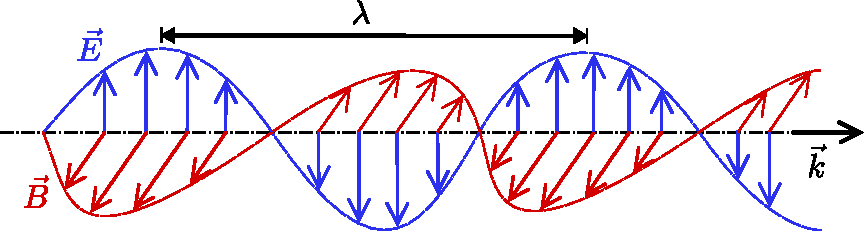
\psfig{file=fig/fig-onda-electromagnetica.pdf,height=3cm,angle=0}}
\caption{Campos el'ectrico y magn'etico de una onda electromagn'etica plana monocrom'atica. Adaptada a partir de \href{http://commons.wikimedia.org/wiki/File:Onde_electromagnetique.svg}{esta} figura original.}
\label{ondaem}
\end{figure}

\subsubsection{Vector de Poynting}
Evaluamos el vector de Poynting (\ref{defPoy}) para la soluci'on de onda plana monocrom'atica reci'en analizada. Usando (\ref{defPoy}), \eqref{BkE} y \eqref{rdoem} podemos escribir
\begin{eqnarray}
 \vec{S}&=&\vec{E}\times\vec{H} \\
&=&\frac{1}{\mu}\,\vec{E}\times\vec{B} \\
&=&\frac{1}{\mu}\,\vec{E}\times\left[\frac{1}{\omega}\,\vec{k}\times\vec{E}
\right] \\
&=&\frac{1}{\mu\omega}\,\vec{E}^2\,\vec{k}\\
&=&\frac{1}{\mu c}\,\vec{E}^2\,\hat{k}. \label{Sop}
\end{eqnarray}
Encontramos de este modo que el campo electromagn'etico correspondiente a la onda plana estudiada \textit{transporta energ'ia en la direcci'on del vector de onda $\vec{k}$}. Su magnitud, aunque siempre no-negativa, var'ia en el tiempo y con la posici'on, ya que $\vec{E}=\vec{E}(\vec{x},t)$. Como la onda considerada es peri'odica, de periodo $T=2\pi/\omega$, es usual considerar el \textbf{promedio del vector de Poynting en un periodo de oscilaci'on}\footnote{Si $f(t)$ es una funci'on del tiempo, entonces definimos su promedio entre $t=0$ y $t=T$ como 
\begin{equation}
\left<f\right>:=\frac{1}{T}\int_0^Tf(t)\,dt.
\end{equation}}
Para la onda sinusoidal (\ref{ecuc-max-solu1}) encontramos entonces que
\begin{equation}\label{Sprom}
\langle\vec{S}\rangle=\frac{1}{2\mu c}\,\vec{E}_0^2\,\hat{k}.
\end{equation}
Esto implica que a trav'es de una superficie de 'area $A$ transversal al vector de onda $\vec{k}$, la onda transporta energ'ia a una tasa (potencia) promedio (en una oscilaci'on) de 
\begin{equation}
 \left<P\right>=\frac{A}{2\mu c}\,\vec{E}_0^2.
\end{equation}

\subsubsection{Densidad de Energ'ia}
An'alogamente, calculamos la densidad de energ'ia electromagn'etica, usando la expresi'on (\ref{uDEHB}):
\begin{eqnarray}
 u&=&\frac{1}{2}\left(\varepsilon\vec{E}^2+\frac{1}{\mu}\vec{B}^2\right)\\
&=&\frac{1}{2}\left(\varepsilon\vec{E}^2+\frac{1}{\mu c^2}\vec{E}^2\right)\\
&=&\frac{1}{2}\left(\varepsilon\vec{E}^2+\varepsilon\vec{E}^2\right)\\
&=&\varepsilon\vec{E}^2. \label{uepE2}
\end{eqnarray}
Similarmente al caso del vector de Poynting, la densidad de energ'ia (siempre no-negativa) var'ia en el tiempo y punto a punto. 
Usando \eqref{uepE2} podemos reescribir el vector de Poynting (\ref{Sop}) como
\begin{equation}
 \vec{S}=u\,c\hat{k}.
\end{equation}
Note que esta expresi'on es an'aloga a $\vec{J}=\rho\vec{v}$ que relaciona la densidad de corriente asociada al movimiento de una densidad $\rho$ (de carga o masa, por ejemplo) con velocidad $\vec{v}$ (``flujo convectivo").

Para la onda peri'odica considerada, podemos calcular la densidad de energ'ia promedio, obteniendo
\begin{equation}\label{uprom}
\left<u\right>=\frac{\varepsilon}{2}\vec{E}_0^2.
\end{equation}

\begin{figure}[!h]
\centerline{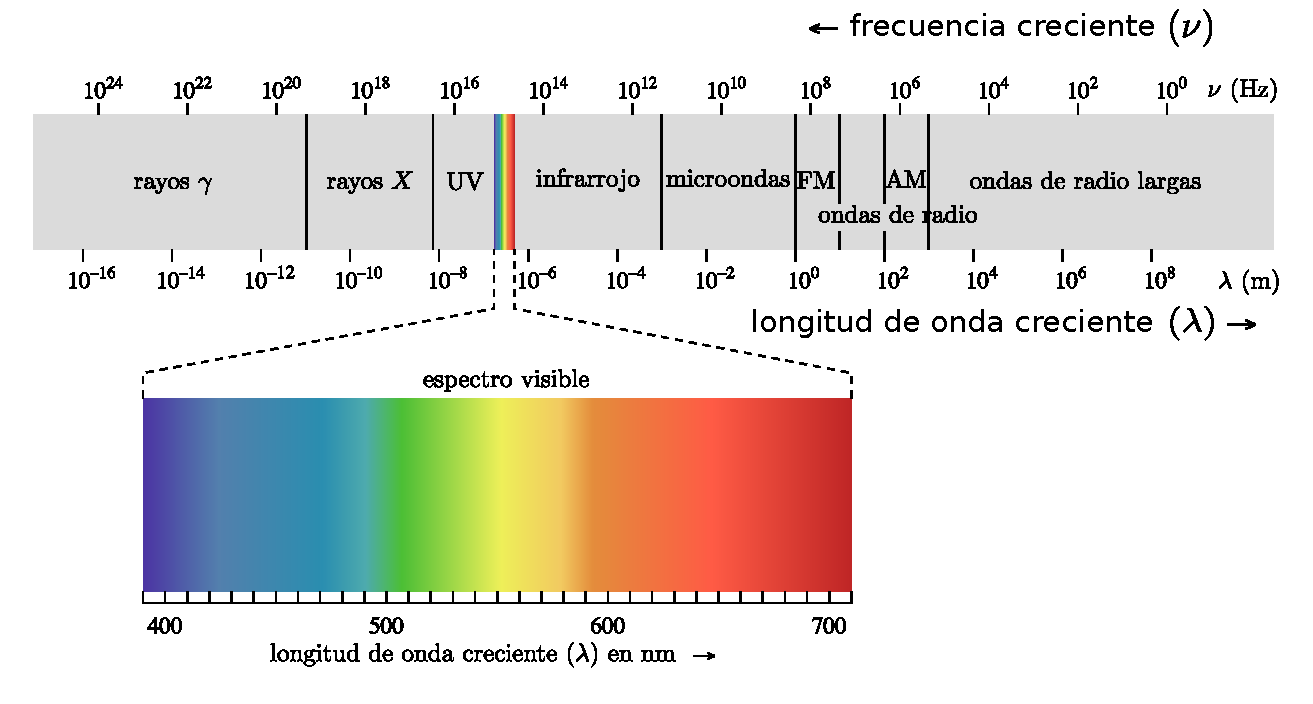
\psfig{file=fig/fig-EM_spectrum_es.pdf,height=7cm,angle=0}}
\caption{Espectro electromagn'etico. Adaptada a partir de \href{http://commons.wikimedia.org/wiki/File:EM_spectrum_es.svg}{esta} figura original.}
\label{fig:EMS}
\end{figure}

\subsection{Ondas electromagn'eticas en la materia}
\subsection{'Indices de reflexi'on y refracci'on}
\subsection{Gu'ias de onda y cavidades resonantes}


\section{Potenciales y transformaciones de gauge}

Las ecuaciones de Maxwell conforman un conjunto de 8 ecuaciones diferenciales
parciales para las 6 componentes del campo electromagn'etico. A menudo es
\textit{conveniente} reducir el n'umero de variables. Esto puede ser conseguido
expresando los campos en t'erminos de \textbf{potenciales electromagn'eticos},
de modo que \textit{las ecuaciones homog'eneas de Maxwell sean satisfechas
autom'aticamente} y el n'umero de campos a determinar se reduce a 4. Estos
potenciales se reducen en los casos estacionarios al conocido potencial
electrost'atico y al potencial vectorial magn'etico.

En el caso din'amico general, de (\ref{max2}) podemos concluir que $\vec{B}$
puede ser derivado de un \textbf{potencial vectorial}:
\begin{eqnarray}\label{defA2}
\boxed{\vec{B}=\vec{\nabla}\times \vec{A}.}
\end{eqnarray}
Usando esto en (\ref{max4}), obtenemos:
\begin{equation}
\vec{\nabla}\times \vec{E} = -  \frac{\partial\ }{\partial
t}(\vec{\nabla}\times\vec{A}) = -\vec{\nabla}\times
\frac{\partial\vec{A}}{\partial t},
\end{equation}
es decir,
\begin{eqnarray}
\vec{\nabla}\times \left[ \vec{E} + \frac{\partial \vec{A}}{\partial t} \right]
= \vec{0}.
\end{eqnarray}
De aqu'i vemos que el campo vectorial dado por la suma $\vec{E} + {\partial
\vec{A}}/{\partial t}$ puede ser escrito como gradiente de un campo escalar, esto es:
\begin{equation}
\vec{E} + \frac{\partial \vec{A}}{\partial t}= - \vec{\nabla}\phi ,
\end{equation}
de donde
\begin{equation}\label{defphi2}
\boxed{\vec{E} =   - \vec{\nabla}\phi - \frac{\partial \vec{A}}{\partial t}.}
\end{equation}
Las ecuaciones (\ref{defA2}) y (\ref{defphi2}) muestran que el campo
electromagn\'etico puede ser escrito en t\'erminos de un potencial vectorial
$\vec{A}$ y de un potencial escalar $\phi$. Sin embargo, estas funciones
\textit{no son 'unicas} para $\vec{E}$ y $\vec{B}$ dados. Es f\'acil verificar
que el campo electromagn\'etico (y consecuentemente todas las predicciones de la
teor'ia electromag\'etica) permanece invariante (es decir, con igual valor) bajo las
siguientes transformaciones de los potenciales,
\begin{equation}\marginnote{Transformaciones de gauge}\label{tgg}
\boxed{{\vec{A}}' = \vec{A} - \vec{\nabla}{\chi}, \qquad \phi' =\phi +
\frac{\partial \chi}{\partial t},}
\end{equation}
conocidas como \textbf{transformaciones de gauge} y donde $\chi=\chi(\vec{x},t)$
es una funci\'on escalar \textit{arbitraria} del espaciotiempo\footnote{La invariancia
de la teor'ia electromagn\'etica bajo transformaciones de gauge
desempe\~na un rol muy importante. La generalizaci\'on de esta propiedad de
invariancia a \textbf{grupos de simetr'ia interna} permiti\'o formular
teor'ias consistentes para las \textbf{interacciones d\'ebiles} unificadas con la electromagn\'etica (\textbf{electrod\'ebil}) y para la \textbf{interacci\'on fuerte}
(\textit{cromodin\'amica cu\'antica}). La \textbf{interacci'on gravitacional} tambi\'en puede ser descrita, con algunas peculiaridades, como una \textit{teor'ia de gauge}.}.

\subsubsection{Ecuaciones de Maxwell inhomog'eneas en t'erminos de los
potenciales}
Consideremos el caso de un medio lineal, is'otropo y homog'eneo. Usando (\ref{defA2}) y (\ref{defphi2}) en las ecuaciones inhomog'eneas (\ref{max1}) y (\ref{max3}) encontramos:
\begin{equation}\label{emiap1}
 \nabla^2\phi+\frac{\partial\ }{\partial t}\left(\vec{\nabla}\cdot\vec{A}\right)=-\frac{\rho}{\varepsilon},
\end{equation}
\begin{equation}\label{emiap2}
 \nabla^2\vec{A}-\frac{1}{c^2}\frac{\partial^2\vec{A}}{\partial t^2}-\vec{\nabla}\left(\vec{\nabla}\cdot\vec{A}+\frac{1}{c^2}\frac{\partial\phi }{\partial t}\right)=-\mu\,\vec{J}.
\end{equation}
De esta forma, hemos reducido las ecuaciones de Maxwell a un conjunto de 4 ecuaciones diferenciales parciales para los 4 potenciales. Sin embargo, estas ecuaciones no determinan completamente los potenciales, puesto que las transformaciones de gauge \eqref{tgg} \textit{dejan invariantes} \eqref{emiap1} y \eqref{emiap1}. Esto es natural ya que estas ecuaciones dependen en realidad de los campos el'ectrico y magn'etico, y como vimos las transformaciones de gauge no cambian los valores de estos campos. Adem'as, las ecuaciones \eqref{emiap1} y \eqref{emiap1} est'an \textit{acopladas}, en el sentido que cada una de estas ecuaciones involucra ambos potenciales electromagn'eticos.

Es posible explotar la ``\textbf{libertad de gauge}'' de la electrodin'amica (es decir, el hecho que los potenciales no son 'unicos) para \textit{simplificar algunos c'alculos}. Una forma de hacer esto es trabajar con potenciales que satisfagan alguna condici'on extra o \textbf{gauge}. De hecho, el imponer condiciones extras a los potenciales no s'olo es conveniente, sino tambi'en \textit{necesario}, ya que las ecuaciones \eqref{emiap1} y \eqref{emiap1} no determinan en forma 'unica los campos $\phi$ y $\vec{A}$. Es posible imponer infinitos gauges diferentes para los potenciales (siempre que sean consistentes con las ecuaciones de Maxwell), pero existen algunos de especial utilidad y popularidad.

\subsubsection{Gauge de Coulomb}
Si el potencial vectorial satisface
\begin{equation}\marginnote{Gauge de Coulomb}\label{gaugeC}
\boxed{ \vec{\nabla}\cdot\vec{A}\stackrel{!}{=}0,}
\end{equation}
se dice que se satisface el \textbf{gauge de Coulomb}, \textbf{gauge de radiaci'on} o \textbf{gauge transversal}. En este caso (\ref{emiap1}) y (\ref{emiap2}) se reducen a
\begin{equation}\label{emiap1GC}
 \nabla^2\phi=-\frac{\rho}{\varepsilon},
\end{equation}
\begin{equation}\label{emiap2GC}
 \nabla^2\vec{A}-\frac{1}{c^2}\frac{\partial^2\vec{A}}{\partial t^2}=-\mu\,\vec{J}+\frac{1}{c^2}\vec{\nabla}\left(\frac{\partial\phi }{\partial t}\right).
\end{equation}

Para probar que \textit{siempre es posible imponer la condici'on de gauge de Coulomb}, podemos considerar el caso en que inicialmente se trabaje con potenciales $\phi_0$ y $\vec{A}_0$ que no satisfacen la condici'on (\ref{gaugeC}), es decir, $\vec\nabla\cdot\vec{A}_0\neq 0$, y luego demostrar que es posible realizar una transformaci'on de gauge (\ref{tgg}) con una funci'on $\chi$ tal que los nuevos potenciales s'i satisfagan (\ref{gaugeC}). Usando (\ref{tgg}b) requerimos entonces que el nuevo potencial vectorial satisfaga
\begin{equation}
\vec\nabla\cdot\vec{A}=\vec\nabla\cdot(\vec{A}_0-\vec\nabla\chi)\stackrel{!}{=}0.
\end{equation}
Esto implica, como condici'on necesaria y suficiente, que la funci'on $\chi$ debe satisfacer 
\begin{equation}\label{ePchi}
\nabla^2\chi=\vec\nabla\cdot\vec{A}_0,
\end{equation}
es decir, la ecuaci'on de Poisson con una ``fuente'' conocida ($\vec\nabla\cdot\vec{A}_0$, dados los potenciales originales). Ya que han sido demostrados \textbf{teoremas de existencia} para esta ecuaci'on, es decir, que ella siempre tiene soluciones, queda demostrado que es \textit{posible} imponer el gauge de Coulomb. Note, sin embargo, que la funci'on $\chi$ que determina los nuevos potenciales que satisfacen el gauge de Coulomb \textit{no es 'unica}, ya que si $\chi_1$ es soluci'on de (\ref{ePchi}) entonces $\chi_2=\chi_1+\tilde\chi$ tambi'en es soluci'on, siempre que $\tilde\chi$ sea una soluci'on de la ecuaci'on de Laplace ($\nabla^2\tilde\chi=0$). Existe entonces una ``\textbf{libertad remanente}'' para seguir realizando transformaciones de gauge, generadas por funciones $\tilde\chi$ que satisfacen la ecuaci'on de Laplace, y que permiten imponer algunas condiciones\footnote{Ojo: no \textit{cualquier} condici'on, sino aquellas que sean compatibles con el resto de las condiciones, y con las ecuaciones de Maxwell.} adicionales a los potenciales, siempre dentro de la ``familia de potenciales'' que satisface el gauge de Coulomb.

Una de las conveniencias de este gauge es que \textit{la ecuaci'on (\ref{emiap1GC}) tiene la misma forma que en el caso electrost'atico}\footnote{Se dice por esto que es ``\textit{coulombiano}'', de ah'i uno de los nombres asociados a este gauge.}. Debido a esto, y usando la ``libertad remanente'' mencionada anteriormente, es posible elegir\footnote{!`Pruebe esta afirmaci'on!.} el potencial escalar de la forma siguiente:
\begin{equation}\label{phiGC}
\boxed{ \phi(\vec{x},t)=\frac{1}{4\pi\varepsilon}\int\frac{\rho(\vec{x}',t)}{\left|\vec{x}-\vec{x}'\right|}dV'.}
\end{equation}
Esta soluci'on para el potencial puede entonces ser reemplazada en el lado derecho de \eqref{emiap2GC}. 
%Sin embargo, un c'alculo sencillo muestra que este 'ultimo t'ermino cancela la \textit{componente irrotacional} (``longitudinal'') de la corriente. En efecto, asumiendo que las fuentes son localizadas, podemos usar el resultado descrito en el ap'endice \ref{Apcamps} y separar la densidad de corriente en una componente longitudinal,  $\vec{J}_{\rm l}$, (o irrotacional, con $\vec\nabla\times\vec{J}_{\rm l}=0$) y una transversal,  $\vec{J}_{\rm t}$, (o solenoidal, con $\vec\nabla\cdot\vec{J}_{\rm t}=0$):
%\begin{equation}
% \vec{J}=\vec{J}_{\rm l}+\vec{J}_{\rm t},
%\end{equation}
%con
%\begin{equation}
% \vec{J}_{\rm l} =-\frac{1}{4\pi}\vec\nabla\int\frac{(\vec\nabla\cdot\vec{J})(\vec{x}')}{|\vec{x}-\vec{x}'|}dV',
%\end{equation}
%\begin{equation}
% \vec{J}_{\rm t} =\frac{1}{4\pi}\vec\nabla\times\int\frac{(\vec\nabla\times\vec{J})(\vec{x}')}{|\vec{x}-\vec{x}'|}dV'.
%\end{equation}
A partir de (\ref{phiGC}), y usando la ecuaci'on de continuidad, podemos escribir el segundo t'ermino del lado derecho de \eqref{emiap2GC} s'olo en t'erminos de la densidad de corriente, ya que
\begin{eqnarray}
\vec{\nabla}\left(\frac{\partial\phi }{\partial t}\right)&=&  \vec{\nabla}\frac{\partial\ }{\partial t}\left(\frac{1}{4\pi\varepsilon}\int\frac{\rho(\vec{x}',t)}{\left|\vec{x}-\vec{x}'\right|}dV'\right) \\
&=&  \frac{1}{4\pi\varepsilon}\vec{\nabla}\int\frac{\frac{\partial\rho }{\partial t}(\vec{x}',t)}{\left|\vec{x}-\vec{x}'\right|}dV' \\
&=& - \frac{1}{4\pi\varepsilon} \vec{\nabla}\int\frac{(\vec{\nabla}'\cdot\vec{J}')}{\left|\vec{x}-\vec{x}'\right|}dV' .%\\
%&=& \frac{1}{\varepsilon}\vec{J}_{\rm l}.
\end{eqnarray}
Con esto, la ecuaci'on (\ref{emiap2GC}) se reduce a
\begin{equation}\label{emiap3GC}
\boxed{\nabla^2\vec{A}-\frac{1}{c^2}\frac{\partial^2\vec{A}}{\partial t^2}=-\mu\,\vec{J}_{\rm T},}
\end{equation}
donde hemos introducido la \textbf{componente transversal de la densidad de corriente}
\begin{align}
\vec{J}_{\rm T} &:= \vec{J}-\frac{1}{c^2\mu}\vec{\nabla}\left(\frac{\partial\phi }{\partial t}\right) \\
&= \vec{J}+\frac{1}{4\pi} \vec{\nabla}\int\frac{(\vec{\nabla}'\cdot\vec{J}')}{\left|\vec{x}-\vec{x}'\right|}dV'.
\end{align}
Se dice que este campo es \textit{transversal} porque satisface
\begin{equation}
\vec\nabla\cdot\vec{J}_{\rm T}\equiv 0.
\end{equation}

En resumen, \textit{en el gauge de Coulomb el potencial vectorial satisface la  \textit{ecuaci'on de onda inhomog'enea}, con un t'ermino fuente determinado s'olo por la componente transversal de la densidad de corriente}. Adem'as, en este gauge  s'olo el potencial vectorial contribuye a los \textbf{campos radiativos}\footnote{Como veremos en el cap'itulo \ref{caprad}, se dice que un campo electromagn'etico es radiativo si su contribuci'on a la energ'ia radiada muy lejos de las fuentes (``en el infinito'') es no nula.}. En cambio, el potencial escalar \eqref{phiGC} es no-radiativo como consecuencia de que su valor decae al menos tan r'apido como $1/r$ a grandes distancias de la fuente.

El gauge de Coulomb es a menudo usado en regiones donde no hay fuentes presentes. En este caso es posible elegir $\phi=0$, ver \eqref{phiGC}, de modo que toda la informaci'on del campo electromagn'etico est'a contenida en el potencial vectorial $\vec{A}$.


\subsubsection{Gauge de Lorenz}
Otro gauge com'un es el \textbf{gauge de Lorenz}\footnote{Nombrado en recuerdo de Ludvig Valentin Lorenz (1829-1891): Matem'atico y F'isico Dan'es. Ver \url{http://es.wikipedia.org/wiki/Ludvig_Lorenz}, quien consider'o esta elecci'on en 1867.}, que usualmente es escrito como
\begin{equation}\marginnote{Gauge de Lorenz}\label{gLorenz}
\boxed{\frac{1}{c^2}\frac{\partial\phi}{\partial t}+\vec{\nabla}\cdot\vec{A}\stackrel{!}{=}0,}
\end{equation}
y que \textit{permite desacoplar las ecuaciones} (\ref{emiap1}) y (\ref{emiap2}).
En efecto, si (\ref{gLorenz}) es satisfecha entonces (\ref{emiap1}) y (\ref{emiap2}) se reducen a
\begin{equation}\label{emiap1gL}
 \nabla^2\phi-\frac{1}{c^2}\frac{\partial^2\phi}{\partial t^2}=-\frac{\rho}{\varepsilon},
\end{equation}
\begin{equation}\label{emiap2gL}
 \nabla^2\vec{A}-\frac{1}{c^2}\frac{\partial^2\vec{A}}{\partial t^2}=-\mu\,\vec{J},
\end{equation}
o, introduciendo el \textbf{operador de onda} (u operador de  d'\,Alembert\footnote{Jean Le Rond d'\,Alembert (1717-1783): matem'atico, fil'osofo y enciclopedista franc'es. Ver \url{http://es.wikipedia.org/wiki/Jean_le_Rond_d\%27Alembert}.}), 
$\Box:= c^{-2}{\partial^2}/{\partial t^2}-\nabla^2$,
\begin{equation}\label{emiap1gL2}
 \Box\phi=\frac{\rho}{\varepsilon},
\end{equation}
\begin{equation}\label{emiap2gL2}
 \Box\vec{A}=\mu\,\vec{J}.
\end{equation}

An'alogamente al caso del gauge de Coulomb, puede probarse que \textit{el gauge de Lorenz siempre puede ser impuesto}, considerando que inicialmente se usen potenciales ($\phi_0$ y $\vec{A}_0$) que no lo satisfacen, y mostrando que puede encontrarse una funci'on $\chi$ que genere la transformaci'on de gauge apropiada para que los nuevos potenciales s'i la satisfagan. En este caso, la condici'on sobre la funci'on $\chi$ requerida es que
\begin{eqnarray}
0&\stackrel{!}{=}&\frac{1}{c^2}\frac{\partial\phi}{\partial t}+\vec{\nabla}\cdot\vec{A} \\
&=&\frac{1}{c^2}\frac{\partial\ }{\partial t}\left(\phi_0+\frac{\partial\chi}{\partial t}\right)+\vec{\nabla}\cdot\left(\vec{A}_0-\vec\nabla\chi\right) \\
&=&\left(\frac{1}{c^2}\frac{\partial\phi_0}{\partial t} +\vec{\nabla}\cdot\vec{A}_0\right) +\frac{1}{c^2}\frac{\partial^2\chi }{\partial t^2}-\nabla^2\chi,
\end{eqnarray}
es decir, que satisfaga la ecuaci'on de onda inhomog'enea:
\begin{equation}
\Box\chi=-\left(\frac{1}{c^2}\frac{\partial\phi_0}{\partial t} +\vec{\nabla}\cdot\vec{A}_0\right).
\end{equation}
La existencia de soluciones de esta ecuaci'on est'a garantizada. An'alogamente al caso del gauge de Coulomb, la funci'on buscada no es 'unica, sino que existe una libertad remanente para realizar transformaciones de gauge ``dentro del gauge de Lorenz'', generadas por funciones $\tilde\chi$ que satisfagan la ecuaci'on de onda, $\Box\tilde\chi=0$. 

El gauge de Lorenz es usado com'unmente en el contexto de la teor'ia de Especial de la Relatividad, ya que en el vac'io (cuando $\varepsilon=\varepsilon_0$ y $\mu=\mu_0$ y por lo tanto $c=c_0$) la condici'on (\ref{gLorenz}) as'i como (\ref{emiap1gL2}) y (\ref{emiap2gL2}), \textit{mantienen su forma inalterada en cualquier sistema de referencia inercial} (son \textit{covariantes} bajo transformaciones de Lorentz). Esto tiene como consecuencia que toda expresi'on que involucre a los potenciales electromag'eticos (que satisfagan el gauge de Lorenz) tendr'a la \textit{misma forma en todo Sistema de Referencia Inercial}. Esto no ocurre, por ejemplo, si se usan potenciales que satisfagan el gauge de Coulomb.
\newpage
\appendix
\chapter{Coordenadas curvilineas}

\section{Coordenadas Cartesianas}
\noindent Vector
\begin{eqnarray}
\vec{A}
&=& A_x{\hat x} + A_y {\hat y} + A_z {\hat z}
\end{eqnarray}
Gradiente:
\begin{eqnarray}
 \vec\nabla\Psi&=&{\partial\Psi\over \partial x} {\hat x} + {\partial\Psi\over
\partial y} {\hat y}   + {\partial\Psi\over \partial z} {\hat z}
\end{eqnarray}
Divergencia
\begin{eqnarray}
 \vec\nabla \cdot \vec{A}
&=& \frac{\partial  A_x}{\partial x}+\frac{\partial  A_y}{\partial y}+\frac{\partial  A_z}{\partial z}
\end{eqnarray}
Rotor:
\begin{eqnarray}
\vec\nabla \times  \vec{A}
&=&   \left({\partial A_z \over \partial y} - {\partial A_y \over
\partial z}\right)  {\hat x}  +
   \left({\partial A_x \over \partial z} - {\partial A_z \over
\partial x}\right)  {\hat y}  +
   \left({\partial A_y \over \partial x} - {\partial A_x \over
\partial y}\right)  {\hat z}
\end{eqnarray}
Laplaciano
\begin{eqnarray}
 \nabla^2 \Psi
&=& {\partial^2\Psi\over \partial x^2} + {\partial^2\Psi\over \partial y^2} +
{\partial^2\Psi\over \partial z^2}
\end{eqnarray}
Desplazamiento:
\begin{eqnarray}
 d \vec{x} &=& dx {\hat x} + dy {\hat y} + dz {\hat z}
\end{eqnarray}
Elemento de superficie:
\begin{eqnarray}
 d \vec{S} &=& dy\,dz\, {\hat x} + dx\,dz\, {\hat y} +
dx\,dy\, {\hat z}
\end{eqnarray}
Elemento de volumen:
\begin{eqnarray}
 dV &=& dx\,dy\,dz
\end{eqnarray}

\section{Coordenadas Cil'indricas}
Definici'on:
\begin{equation}
    x  =  \rho\cos\varphi , \qquad
    y  =  \rho\sin\varphi , \qquad
    z =  z
\end{equation}
\begin{equation}
    \rho  =  \sqrt{x^2 + y^2} , \qquad
    \varphi  = \arctan{(y/x)}, \qquad
     z=  z
\end{equation}
Vector
\begin{equation}
\vec{A} =A_\rho {\hat \rho} + A_\varphi {\hat \varphi} +
A_z {\hat z}
\end{equation}
Gradiente:
\begin{eqnarray}
 \vec\nabla\Psi&=&{\partial\Psi\over \partial \rho} {\hat \rho}
  + {1 \over \rho}{\partial\Psi\over \partial \varphi} {\hat \varphi}
  + {\partial\Psi\over \partial z} {\hat z}
\end{eqnarray}
Divergencia
\begin{eqnarray}
 \vec\nabla \cdot \vec{A}
&=&  {1 \over \rho}{\partial \left( \rho A_\rho  \right) \over \partial
\rho}  + {1 \over \rho}{\partial A_\varphi \over \partial \varphi}
  + {\partial A_z \over \partial z}
\end{eqnarray}
Rotor:
\begin{eqnarray}
\vec\nabla \times  \vec{A}
&=&   \left({1 \over \rho}{\partial A_z \over \partial \varphi}
    - {\partial A_\varphi \over \partial z}\right)  {\hat \rho} +
\left({\partial A_\rho \over \partial z} - {\partial A_z \over
\partial \rho}\right)  {\hat \varphi} \nonumber\\
&&+  {1 \over \rho}\left({\partial \left( \rho A_\varphi \right) \over
\partial \rho}     - {\partial A_\rho \over \partial \varphi}\right) {\hat z}
\end{eqnarray}
Laplaciano
\begin{eqnarray}
 \nabla^2 \Psi
&=& {1 \over \rho}{\partial \over \partial \rho}\left(\rho {\partial\Psi\over
\partial \rho}\right)
  + {1 \over \rho^2}{\partial^2\Psi\over \partial \varphi^2}
  + {\partial^2\Psi\over \partial z^2} \\
\end{eqnarray}
Desplazamiento:
\begin{eqnarray}
 d \vec{x}
 &=& d\rho {\hat \rho} + \rho d\varphi {\hat \varphi} +dz {\hat z}
\end{eqnarray}
Elemento de superficie:
\begin{eqnarray}
 d \vec{S}
&=& \rho\, d\varphi\, dz\, {\hat \rho} + d\rho
\,dz\, {\hat \varphi} +  \rho \,d\rho\, d\varphi \, {\hat z}
\end{eqnarray}
Elemento de volumen:
\begin{eqnarray}
 dV
 &=& \rho\, d\rho\, d\varphi\, dz
\end{eqnarray}

\section{Coordenadas Esf'ericas}
Definici'on:
\begin{equation}
    x  =  r\sin\theta\cos\varphi, \qquad
    y  =  r\sin\theta\sin\varphi , \qquad
    z  =  r\cos\theta
\end{equation}
\begin{equation}
    r  =  \sqrt{x^2 + y^2 + z^2} , \quad
    \theta  =  \arccos(\frac{z}{r}) = \arctan{\frac{\sqrt{x^2+y^2}}{z}}, \quad
    \varphi  =  \arctan{(y/x)}
\end{equation}
Vector
\begin{eqnarray}
\vec{A}
&=& A_r {\hat r} + A_\theta {\hat \theta} +
A_\varphi {\hat \varphi}
\end{eqnarray}
Gradiente:
\begin{eqnarray}
 \vec\nabla\Psi
 &=& {\partial\Psi\over \partial r} {\hat r}
  + {1 \over r}{\partial\Psi\over \partial \theta} {\hat \theta}
  + {1 \over r\sin\theta}{\partial\Psi\over \partial \varphi} {\hat \varphi}
\end{eqnarray}
Divergencia
\begin{eqnarray}
 \vec\nabla \cdot \vec{A}
&=& {1 \over r^2}{\partial \left( r^2 A_r \right) \over \partial r}
  + {1 \over r\sin\theta}{\partial \over \partial \theta} \left(
A_\theta\sin\theta \right)
  + {1 \over r\sin\theta}{\partial A_\varphi \over \partial \varphi}
\end{eqnarray}
Rotor:
\begin{eqnarray}
\vec\nabla \times  \vec{A}
&=&  {1 \over r\sin\theta}\left({\partial \over \partial \theta}
\left( A_\varphi\sin\theta \right)    - {\partial A_\theta \over \partial
\varphi}\right) {\hat r} \nonumber\\
&&+    {1 \over r}\left({1 \over \sin\theta}{\partial A_r \over \partial
\varphi} - {\partial \over \partial r} \left( r A_\varphi \right) \right)
 {\hat \theta}  +   {1 \over r}\left({\partial \over \partial r} \left( r
A_\theta
\right)  - {\partial A_r \over \partial \theta}\right)  {\hat \varphi}
\end{eqnarray}
Laplaciano
\begin{eqnarray}
 \nabla^2 \Psi
&=&  {1 \over r^2}{\partial \over \partial r}\left(r^2 {\partial\Psi\over
\partial r}\right)   + {1 \over r^2\sin\theta}{\partial \over \partial
\theta}\left(\sin\theta {\partial\Psi\over \partial \theta}\right)
  + {1 \over r^2\sin^2\theta}{\partial^2\Psi\over \partial \varphi^2}
\end{eqnarray}
Desplazamiento:
\begin{eqnarray}
 d \vec{x}
&= & dr {\hat r} + rd\theta {\hat \theta} +r\sin\theta d\varphi {\hat \varphi}
\end{eqnarray}
Elemento de superficie:
\begin{eqnarray}
 d \vec{S}
&=& r^2 \sin\theta \,d\theta \,d\varphi \, {\hat r} + r\sin\theta
\,dr\,d\varphi \, {\hat \theta} +  r\,dr\,d\theta\, {\hat \varphi}
\end{eqnarray}
Elemento de volumen:
\begin{eqnarray}
 dV
&=& r^2\sin\theta \,dr\,d\theta\, d\varphi
\end{eqnarray}

\newpage
\chapter{Campos vectoriales, rotores y divergencias}\label{Apcamps}
Todo campo vectorial en 3 dimensiones, continuo y diferenciable (de clase $C^2$), y \textit{que se anula en el infinito m'as r'apidamente que} $r^{-3/2}$, est'a 'unicamente determinado por ``sus fuentes'': su rotor (``densidad de circulaci'on'') y por su divergencia (``densidad de fuente'').

Considere un campo vectorial $\vec V(\vec x)$, definimos su divergencia y su
rotor, respectivamente, por
\begin{equation}
 D(\vec x):=\vec\nabla\cdot\vec V, \qquad \vec C(\vec x):=\vec\nabla\times\vec
V. \label{divrot}
\end{equation}
Entonces es posible descomponer $\vec V(\vec x)$ del modo siguiente:
\begin{equation}
 \vec V(\vec x)=-\vec\nabla\phi+\vec\nabla\times\vec A, \label{decomp1}
\end{equation}
con
\begin{equation}
 \phi(\vec x):=\frac{1}{4\pi}\int_{R^3}\frac{D(\vec x')}{\left|\vec x-\vec
x'\right|}\,dV',
\end{equation}
\begin{equation}
 \vec A(\vec x):=\frac{1}{4\pi}\int_{R^3}\frac{\vec C(\vec x')}{\left|\vec
x-\vec x'\right|}\,dV' .
\end{equation}
En efecto:
\begin{eqnarray}
\vec\nabla\cdot\vec
V&=&\vec\nabla\cdot\left(-\vec\nabla\phi+\vec\nabla\times\vec
A\right) \\
&=&-\nabla^2\phi \\
&=&- \frac{1}{4\pi}\nabla^2\int_{R^3}\frac{D(\vec x')}{\left|\vec x-\vec
x'\right|}\,dV'\\
&=&- \frac{1}{4\pi}\int_{R^3}D(\vec x')\nabla^2\frac{1}{\left|\vec x-\vec
x'\right|}\,dV'\\
&=&- \frac{1}{4\pi}\int_{R^3}D(\vec
x')\left(-4\pi\delta^{(3)}(\vec x-\vec x')\right)\,dV'\\
&=&\int_{R^3}D(\vec x')\delta^{(3)}(\vec x-\vec x')\,dV'\\
&=&D(\vec x).
\end{eqnarray}
Adem'as
\begin{eqnarray}
\vec\nabla\times\vec
V&=&\vec\nabla\times\left(-\vec\nabla\phi+\vec\nabla\times\vec
A\right) \\
&=& \vec\nabla\times(\vec\nabla\times\vec A) \\
&=& \vec\nabla(\vec\nabla\cdot\vec A) -\nabla^2\vec A\\
&=& \frac{1}{4\pi}\int_{R^3}(\vec
C(\vec x')\cdot\vec\nabla)\vec\nabla\left(\frac{1}{\left|\vec
x-\vec x'\right|}\right)\,dV' -\frac{1}{4\pi}\int_{R^3}\vec
C(\vec x')\nabla^2\left(\frac{1}{\left|\vec
x-\vec x'\right|}\right)\,dV' \\
&=& \frac{1}{4\pi}\int_{R^3}(\vec
C(\vec x')\cdot\vec\nabla)\vec\nabla\left(\frac{1}{\left|\vec
x-\vec x'\right|}\right)\,dV' +\int_{R^3}\vec
C(\vec x')\delta^{(3)}\left(\vec x-\vec x'\right)\,dV' \\
&=& \frac{1}{4\pi}\int_{R^3}(\vec
C(\vec x')\cdot\vec\nabla)\vec\nabla\left(\frac{1}{\left|\vec
x-\vec x'\right|}\right)\,dV' +\vec C(\vec x). \label{rotv}
\end{eqnarray}
Probaremos ahora que el primer t'ermino de (\ref{rotv}) es cero si $\vec C$ es
un campo acotado. Usando notaci'on indicial, tenemos que la (componente
$i$-'esima de la) expresi'on en el primer t'ermino de (\ref{rotv}), puede
escribirse como
\begin{eqnarray}
\int_{R^3}C_j'\partial_j\partial_i\frac{1}{\left|\vec
x-\vec x'\right|}\,dV'
&=&\int_{R^3}C_j'\partial'_j\partial'_i\frac{1}{
\left|\vec x-\vec x'\right|}\,dV'\\
&=&\int_{R^3}\left[\partial'_j\left(C_j'\partial'_i\frac{1}{
\left|\vec x-\vec x'\right|}\right)-(\partial'_jC_j')\partial_i'\frac{1}{
\left|\vec x-\vec x'\right|}\right]\,dV'\\
&=&\int_{R^3}\left[\partial'_j\left(C_j'\partial'_i\frac{1}{
\left|\vec x-\vec x'\right|}\right)+0\right]\,dV'\\
&=&\oint_{\partial R^3}C_j'\partial'_i\frac{1}{\left|\vec x-\vec
x'\right|}\,dS'_j\\
\end{eqnarray}
En el infinito ($\partial R^3$), $|\vec x|\rightarrow \infty$, de modo que
$\frac{1}{\left|\vec x-\vec x'\right|}\sim \frac{1}{r}$,
$\partial_i'\frac{1}{\left|\vec x-\vec x'\right|}\sim \frac{1}{r^2}$. Adem'as
$dS\sim r^2d\Omega$ en el mismo l'imite, de modo que
$\partial_i'\frac{1}{\left|\vec x-\vec x'\right|}dS_j\sim d\Omega$. En otras
palabras, la contribuci'on de $\partial_i'\frac{1}{\left|\vec x-\vec
x'\right|}dS_j$ es finita en el infinito espacial. Por lo tanto, la integral
en (\ref{rotv}) se anular'a si $\vec C\rightarrow\vec 0$ en el infinito.

Hemos as'i verificado que, dada la divergencia y el rotor de un campo vectorial
tridimensional, es posible reconstruir el campo original. Adem'as,
todo campo vectorial tridimensional puede ser descompuesto en un t'ermino
derivado de un campo escalar (de rotor nulo) y un t'ermino derivado de un
potencial vectorial (de divergencia nula). Note, sin embargo, que los campos
``potenciales'' $\phi$ \textit{no son 'unicos} (siempre es posible sumar una
constante al potencial escalar $\phi$ y un gradiente de otro campo escalar al
potencial vectorial $\vec A$).

Por otro lado, el vector $\vec V$ calculado usando (\ref{decomp1}) es el 'unico
que tiene divergencia $D$ y rotor $\vec C$. En efecto, suponga que existen 2
campos $\vec V_1$ y $\vec V_1$ que satisfacen (\ref{divrot}). Definiendo $\vec
W:=\vec V_1-\vec V_2$ encontramos
\begin{equation}
 \vec\nabla\cdot\vec W=0, \qquad \vec\nabla\times\vec W=\vec 0. \label{drW}
\end{equation}
La condici'on (\ref{drW}b) implica que es posible escribir $\vec
W=-\vec\nabla\psi$ con una campo escalar $\psi$. Con esto, (\ref{drW}a) implica
que $\psi$ debe satisfacer la ecuaci'on de Laplace $\nabla^2\psi=0$.

Usando la identidad \textit{primera identidad de Green}:
\begin{equation}
 \oint_{\partial V}\psi \vec\nabla\psi\cdot d\vec S\equiv \int_V
\left[\psi\nabla^2\psi+(\vec\nabla\psi)^2\right]\,dV ,
\end{equation}
encontramos:
\begin{equation}
 \oint_{\partial V}\psi \vec\nabla\psi\cdot d\vec S\equiv \int_V
(\vec\nabla\psi)^2\,dV . \label{iG2}
\end{equation}
La integral del lado izquierdo de (\ref{iG2}) se anula en el caso que $V=R^3$
puesto que la familia de campos vectoriales $\vec V$ considerados decrece m'as
r'apido que $r^{-3/2}$ en el infinito\footnote{Como consecuencia $\psi$
decrece m'as r'apido que $r^{-3/2}$ y $\psi \vec\nabla\psi$ decrece m'as
r'apido que $r^{-2}$, mientras que $d\vec S$ aumenta como $r^2$.}. Finalmente,
la anulaci'on del lado derecho de  (\ref{iG2}) requiere que
$\vec\nabla\psi=\vec 0$, de modo que $\psi$ puede a lo sumo ser una constante.
En este caso, sin embargo, $\vec W=-\vec\nabla\psi=\vec 0$, es decir $\vec
V_1=\vec V_2$.

Como consecuencia de lo anterior, podemos establecer los siguientes resultados
para un campo vectorial $\vec V$ que se anula en el infinito m'as
r'apidamente que $r^{-3/2}$:
\begin{itemize}
\item Si la divergencia y el rotor de un campo vectorial son conocidos y si
este campo no tiene fuentes en el infinito, entonces el campo est'a 'unicamente
determinado
\item Si $\vec\nabla\cdot\vec V\neq 0$ y $\vec\nabla\times\vec V=\vec 0$
entonces $\vec V$ puede ser derivado de un campo escalar: $\vec
V=-\vec\nabla\phi$.
\item Si $\vec\nabla\times\vec V\neq \vec 0$ y $\vec\nabla\cdot\vec V= 0$
entonces $\vec V$ puede ser derivado de un campo vectorial: $\vec
V=\vec\nabla\times\vec A$.
\item $\vec{V}$ puede ser descompuesto como una superposici'on (suma) de un
campo libre de rotaci'on y uno libre de fuentes.
\item Si $\vec\nabla\times\vec V=\vec 0$ y $\vec\nabla\cdot\vec V= 0$ \textit{en
una cierta regi'on}, entonces $\vec V$ puede ser derivado de un potencial $\phi$
que satisface $\nabla^2\phi=0$. Decimos que $\vec V$ es \textit{arm'onico} en
dicha regi'on.
\item Si $\vec\nabla\times\vec V=\vec 0$ y $\vec\nabla\cdot\vec V= 0$ \textit{en
todo el espacio}, entonces $\vec V=\vec 0$.
\end{itemize}


\chapter{Sistemas de Unidades}\label{appuni}
% \section{Tabla de equivalencias para unidades gaussianas y S.I.}
% \begin{tabular}[c]{|l|lll|}
% \hline
% Corriente &  1 statampere & = & $\frac{10}{c}$ ampere\\\hline
% Carga  &  1 statcoulomb & = & $\frac{10}{c}$ coulomb\\\hline
% voltaje &   1 statvolt & $\approx$ & 300 volt\\\hline
% Resistencia  & 1 statohm & $\approx$ & $9\times10^{11}$ ohm\\\hline
% Resistividad & 1 segundo & $\approx$ & $9\times10^{9}$ ohm $\times$
% metro\\\hline
% Capacitancia  & 1 cent'imetro & $\approx$ & $\frac{1}{9\times10^{11}}$
%farad\\\hline
% Campo el'ectrico  & 1 $\frac{dina}{statcoulomb}$ & $\approx$ &
% $3\times10^4\frac{newton}{coulomb}$\\\hline
% Autoinductancia & 1 stathenry & $\approx$ & $9\times10^{11}$ henry\\\hline
% Inducci'on magn'etica  & 1 gauss & $=$ & $10^{-4}$ tesla\\\hline
% Flujo magn'etico  & 1 maxwell & $=$ & $10^{-8}$ tesla$\times$ m$^2$\\\hline
% Intensidad de campo  & 1 oersted & $=$ &
%$\frac{10^3}{4\pi}\frac{ampere}{metro}$
% \\\hline
% \end{tabular}
% 
% \begin{tabular}
% [c]{|l|l|l|l|l|}\hline
% Cantidad & S'imbolo & MKS &  & CGS\\\hline
% Longitud & $l$ & 1m & 10$^2$ & cm\\\hline
% Masa & $m$ & 1kg & 10$^3$ & g\\\hline
% Tiempo & $t$ & 1s & 1 & s\\\hline
% Frecuencia & $\nu$ & 1Hz & 1 & Hz\\\hline
% Fuerza & $F$ & 1N & 10$^{5}$ & dinas\\\hline
% Energ'ia & $U,W$ & 1J & 10$^{7}$ & erg\\\hline
% Potencia & $P$ & 1W & 10$^{7}$ & $\frac{\text{erg}}{\text{s}}$\\\hline
% Carga & $q$ & $1$coulomb & 3$\times10^{9}$ & statcoulombs\\\hline
% Densidad de Carga & $\rho$ & 1$\frac{\text{coulomb}}{\text{m}^3}$ &
% 3$\times10^3$ & $\frac{\text{statcoulombs}}{\text{cm}^3}$\\\hline
% Corriente & $I$ & 1amp & 3$\times10^{9}$ & statamperes\\\hline
% Densidad de Corriente & $J$ & 1$\frac{\text{amp}}{^{\text{m}^2}}$ &
% 3$\times10^{5}$ & $\frac{\text{statamperes}}{\text{cm}^2}$\\\hline
% Campo El'ectrico & $E$ & 1$\frac{\text{volt}}{\text{m}}$ & $\frac{1}%
% {3}\times10^{-4}$ & $\frac{\text{statvolt}}{\text{cm}}$\\\hline
% Potencial & $\phi$ & 1volt & $\frac{1}{300}$ & statvolt\\\hline
% Polarizaci'on & $P$ & 1$\frac{\text{coul}}{\text{m}^2}$ & 3$\times10^{5}$
% & $\frac{\text{momento dipolar}}{\text{cm}^3}$\\\hline
% Desplazamiento & $D$ & 1$\frac{\text{coul}}{\text{m}^2}$ & 12$\pi
% \times10^{5}$ & $\frac{\text{statvolt}}{\text{cm}}$ 'o $\frac
% {\text{statcoulombs}}{\text{cm}^2}$\\\hline
% Conductividad & $\sigma$ & 1$\frac{\text{mho}}{\text{m}}$ & 9$\times10^{9}$ &
% $\frac{1}{\text{s}}$\\\hline
% Resistencia & $R$ & 1ohm & $\frac{1}{9}10^{-11}$ & $\frac{\text{s}}{\text{cm}%
% }$\\\hline
% Capacitancia & $C$ & 1farad & 9$\times10^{11}$ & cm\\\hline
% Inducci'on Magn'etica & $B$ & 1tesla & 10$^4$ & gauss\\\hline
% Magnetizaci'on & $M$ & 1$\frac{\text{ampere}}{\text{m}}$ & 10$^{-3}$ &
% $\frac{\text{momento magn'etico}}{\text{cm}^3}$\\\hline
% Inductancia & $L$ & 1henry & $\frac{1}{9}\times10^{-11}$ &
% \textquestiondown ?\\\hline
% Acci'on & $S$ & kg$\frac{\text{m}^2}{\text{s}}$ & $10^{7}$ &
% g$\frac{\text{cm}^2}{\text{s}}$\\\hline
% \end{tabular}
Los diferentes sistemas de unidades usados en la teor'ia electromagn'etica pueden entenderse en funci'on de la libertad que existe para definir las unidades de carga y campo el'ectrico y magn'etico. Aqu'i discutiremos algunas posibilidades, que incluyen al sistema S.I. y al gaussiano. Discutiremos c'omo estos sistemas de unidades ``separan'' de forma diferente la magnitud de la carga el'ectrica de la de los campos electromagn'eticos. Las cantidades mec'anicas, sin embargo, no son alteradas por estas diferentes formas de separar cargas y campos.

Para esta discusi'on, es conveniente considerar las cantidades puramente mec'anicas relacionadas con las definiciones b'asicas de las cantidades electromagn'eticas. En particular, la ley de Coulomb establece que la fuerza entre dos cargas es proporcional al producto de cargas e inversamente proporcional al cuadrado de la distancia que las separa:
\begin{equation}
 F_{\rm e}\propto\frac{q q'}{r^2}.
\end{equation} 
Las unidades en que se miden las cargas depende del valor de la constante de proporcionalidad,
\begin{equation}
 \vec{F}_{\rm e}=\alpha_1\,\frac{q q'}{r^2}\hat{r}.
\end{equation} 
Esto determina adem'as las unidades del campo el'ectrico que es dado, \textit{por definici'on}\footnote{En pricipio, es posible definir el campo el'ectrico y sus unidades asociadas introduciendo otra constante a elecci'on, por ejemplo, $\vec{E}:=8 \vec{F}_{\rm e}/q$. No exploraremos aqu'i esta posibilidad.}, por $\vec{E}:=\vec{F}_{\rm e}/q$. De esta forma:
\begin{equation}
 [q]=[\alpha_1]^{-1/2}[F]^{1/2}L =[\alpha_1]^{-1/2}M^{1/2}L^{3/2}T^{-1},
\end{equation}
\begin{equation}
 [E]=[\alpha_1]^{1/2}[F]^{1/2}L^{-1}=[\alpha_1]^{1/2}M^{1/2}L^{-1/2}T^{-1}.
\end{equation}
Por otro lado, la fuerza magn'etica entre cargas en movimiento (corrientes) est'an dadas, por ejemplo, por la ley de Biot-Savart:
\begin{equation}
 dF_{\rm m}\propto II' dx \times dx' \frac{1}{r^2}.
\end{equation}
Aqu'i debemos introducir nuevamente una constante, tal que,
\begin{equation}
 dF_{\rm m}=\alpha_2\, II'dx \times dx' \frac{1}{r^2}. \label{dfe}
\end{equation}
El campo magn'etico, es \textit{definido} tal que
\begin{equation}
 d\vec{F}_{\rm m}\propto I'd\vec{x}' \times d\vec{B}.
\end{equation}
En particular, existen sistemas de unidades que difieren en la constante de proporcionalidad de esta definici'on. Introducimos entonces otra constante de modo que
\begin{equation}\label{dFa3}
 d\vec{F}_{\rm m}=\alpha_3\,I'd\vec{x}' \times d\vec{B},
\end{equation}
y as'i
\begin{equation}
 d\vec{B}=\frac{\alpha_2}{\alpha_3} \frac{Id\vec{x}\times\hat{r}}{r^2}.
\end{equation}
Esto implica que
\begin{equation}
[B]=[\alpha_1]^{-1/2}[\alpha_2][\alpha_3]^{-1}M^{1/2}L^{1/2}T^{-2}.
\end{equation}
De la expresi'on (\ref{dFa3}) encontramos, equivalentemente, que la fuerza que ejerce un campo magn'etico sobre cargas puntuales es dado por
\begin{equation}
\vec{F}_{\rm m}=\alpha_3\, q\,\vec{v}\times\vec{B},
\end{equation} 
de modo que la fuerza de Lorentz adopta la forma
\begin{equation}
 \vec{F}=q\left(\vec{E}+\alpha_3\,\vec{v}\times\vec{B}\right).
\end{equation} 
Usando (\ref{dfe}) encontramos en particular que la fuerza entre dos l'ineas de corriente $I$ e $I'$, de largo $L$ y separadas una distancia $d$ es
\begin{equation}
 F=2\alpha_2\,II' \frac{L}{d}.
\end{equation} 
A partir de estas definiciones b'asicas es posible encontrar la forma de las ecuaciones de Maxwell correspondientes, de modo que se satisfaga la ley de Faraday y la ecuaci'on de continuidad. As'i obtenemos:
\begin{equation}
 \vec{\nabla}\cdot\vec{E}=4\pi\alpha_1\rho,
\end{equation} 
\begin{equation}
 \vec{\nabla}\cdot\vec{B}=0,
\end{equation} 
\begin{equation}
 \vec{\nabla}\times\vec{E}+\alpha_3\frac{\partial\vec{B}}{\partial t}=\vec{0},
\end{equation} 
\begin{equation}
 \vec{\nabla}\times\vec{B}=4\pi\frac{\alpha_2}{\alpha_3}\vec{J}+\frac{\alpha_2}{\alpha_1\alpha_3}\frac{
\partial\vec{E}}{\partial t}.
\end{equation} 
En una regi'on libre de fuentes podemos derivar la ecuaci'on de onda para las componentes del campo el'ectrico, obteniendo
\begin{equation}
 \left(\frac{\alpha_2}{\alpha_1}\frac{\partial^2\
}{\partial t^2}-\nabla^2\right)\vec{E} =\vec {0},
\end{equation}
de donde encontramos que la velocidad de la luz es dada por la relaci'on
 \begin{equation}
\frac{\alpha_2}{\alpha_1}=\frac{1}{c^2}.
 \end{equation} 
Ya que $c$ es una cantidad mec'anica, su valor no debe depender del sistema de unidades usado para las cantidades electromagn'eticas. Esto significa que s'olo 2 de las 3 constantes pueden elegirse arbitrariamente, por ejemplo, $\alpha_2$ y $\alpha_3$, mientras que $\alpha_1=\alpha_2c^2$. A continuaci'on resumiremos los dos sistemas de unidades m'as com'unmente usados.

\section{Sistema Internacional de unidades (S.I.)}
En este sistema de unidades se define\footnote{Ver, por ejemplo, la p'agina correspondiente del Instituto Nacional de Est'andars y Tecnolog'ia de Estados Unidos (NIST): \url{http://physics.nist.gov/cuu/Units/ampere.html}.} un Ampere como ``la intensidad de una corriente constante que manteni'endose en dos conductores paralelos, rectil'ineos, de longitud infinita, de secci'on circular despreciable y situados a una distancia de un metro uno de otro en el vac'io, produce una fuerza igual a $2\times 10^{-7}$N por metro de longitud". Esto implica que
\begin{equation}
\alpha_2\stackrel{!}{=} 10^{-7}NA^{-2}=:\frac{\mu_0}{4\pi},
\end{equation}
\begin{equation}
\alpha_3\stackrel{!}{=} 1,
\end{equation}
y adem'as se denota
\begin{equation}
\alpha_1=:\frac{1}{4\pi\varepsilon_0}.
\end{equation}
Por lo tanto, la velocidad de la luz es dada por
\begin{equation}
c=\frac{1}{\sqrt{\varepsilon_0\mu_0}}.
\end{equation}
La tabla \ref{TUSI} resume las ecuaciones de Maxwell en este sistema de unidades y las unidades en que son medidas cada cantidad. 
\begin{table}
\begin{center}
\begin{tabular}{|l|l|}\hline
$\varepsilon_0\vec{\nabla}\cdot\vec{E}=\rho$ & $\left[ \vec{E}
\right] =\frac{\mathbf{N}}{\mathbf{C}}=\frac{\mathbf{V}}{\mathbf{m}}$\\\hline
$\frac{1}{\mu_0}\vec{\nabla}\times \vec{B}-\varepsilon_0\frac{\partial
\vec{E}}{\partial t}= \vec{J}$ &
$\left[\vec{B}\right]=\frac{\mathbf{N}\mathbf{s}}{\mathbf{C}\mathbf{m}}
=\frac{\mathbf{kg}}{\mathbf{C}\mathbf{s}}$\\\hline
$\vec{\nabla}\times \vec{E}+\frac{\partial\vec{B}}{\partial t}=0$ &
$\left[\varepsilon_0\right]=\frac{\mathbf{C}}{\mathbf{m}\mathbf{V}}$\\\hline
$\vec{\nabla}\cdot\vec{B}=0$ & $\left[\mu_0\right]=\frac{\mathbf{N}\mathbf{s}^2}
{\mathbf{C}^2}$\\\hline
$\vec{F}=q\left(\vec{E}+\vec{v}\times\vec{B}\right) $ &
$\left[\vec{A}\right]=\frac{\mathbf{N}}{\mathbf{A}}$\\\hline
$\vec{E}=-\vec{\nabla}\phi-\frac{\partial\vec{A}}{\partial t}$ &
$\left[F\right]=\mathbf{N}$\\\hline
$\vec{B}=\vec{\nabla}\times \vec{A}$ & $\left[\phi\right]=\mathbf{V}$ \\\hline
\end{tabular}
\label{TUSI}
\caption{Resumen Sistema Internacional de Unidades.}
\end{center}
\end{table}


\section{Sistema Gaussiano de Unidades (C.G.S.)}\label{appunid}
En este caso, se impone que
\begin{equation}
 \alpha_1\stackrel{!}{=} 1, \qquad \alpha_3\stackrel{!}{=} \frac{1}{c},
\end{equation}
y como consecuencia
\begin{equation}
\alpha_2=\frac{1}{c^2}.
\end{equation} 
Como resultado, las cargas el'ectricas as'i como los campos electromagn'eticos necesariamente se miden en unidades con exponentes fraccionarios de las magnitudes b'asicas de longitud, tiempo y masa:
\begin{equation}
 \left[q\right]=M^{1/2}L^{3/2}T^{-1}, \qquad
\left[E\right]=\left[B\right]=M^{1/2}L^{-1/2}T^{-1}.
\end{equation} 
Una ventaja relativa de este sistema es que los campos el'ectricos y magn'eticos tienen las mismas unidades. Otra es que en las ecuaciones de Maxwell s'olo aparece \textit{una constante fundamental}, la velocidad de la luz.
\begin{table}
\begin{center}
\begin{tabular}{|c|}\hline
$\vec{\nabla}\cdot\vec{E}=4\pi\rho$ \\\hline
$\vec{\nabla}\times \vec{B}-\frac{1}{c}\frac{\partial\vec{E}}{\partial t}=
\frac{4\pi}{c}\vec{J}$ \\\hline
$\vec{\nabla}\times \vec{E}+\frac{1}{c}\frac{\partial\vec{B}}{\partial t}=0$
\\\hline
$\vec{\nabla}\cdot\vec{B}=0$\\\hline
$\vec{F}=q\left(\vec{E}+\frac{\vec{v}}{c}\times \vec{B}\right)$\\\hline
$\vec{E}=-\vec{\nabla}\phi-\frac{1}{c}\frac{\partial \vec{A}}{\partial
t}$\\\hline
$\vec{B}=\vec{\nabla}\times \vec{A}$\\\hline
\end{tabular}
\label{TUSG}
\caption{Resumen Sistema Gaussiano de Unidades.}
\end{center}
\end{table}

\section{Conversi'on de magnitudes S.I. a Gaussianas}
\begin{equation}
\vec{E}_{\rm SI}=\frac{1}{\sqrt{4\pi\varepsilon_0}}\vec{E}_{\rm G}, \qquad 
\vec{B}_{\rm SI}= \frac{1}{c\sqrt{4\pi\varepsilon_0}}\vec{B}_{\rm G}, \qquad 
q_{\rm SI}=\sqrt{4\pi\varepsilon_0}\,q_{\rm G}
\end{equation}
\begin{equation}
\vec{A}_{\rm SI}=\frac{1}{c\sqrt{4\pi\varepsilon_0}}\,\vec{A}_{\rm G}, \qquad
\phi_{\rm SI}=\frac{1}{\sqrt{4\pi\varepsilon_0}}\,\phi_{\rm G}.
\end{equation}
%\begin{center}
%\begin{tabular}{|lcl|}\hline
%S.I. &$\rightarrow$& Gauss.\\\hline\hline
%$\vec{E}$ & $\rightarrow$& $\frac{\vec{E}}{\sqrt{4\pi\varepsilon_0}}$\\\hline
%$\vec{B}$ & $\rightarrow$& $\frac{\vec{B}}{c\sqrt{4\pi\varepsilon_0}}$\\\hline
%$q$ & $\rightarrow$ & $\sqrt{4\pi\varepsilon_0}q$\\\hline
%$\vec{A}$ & $\rightarrow$ & $\frac{\vec{A}}{c\sqrt{4\pi\varepsilon_0}}$\\\hline
%$\phi$ & $\rightarrow$ & $\frac{\phi}{\sqrt{4\pi\varepsilon_0}}$\\\hline
%$\vec{J}$ & $\rightarrow$ & $ \sqrt{4\pi\varepsilon_0}\vec{J}$\\\hline
%$\rho$ & $\rightarrow$ & $\sqrt{4\pi\varepsilon_0}\rho$\\\hline
%\end{tabular}
%\end{center}

\chapter{Constantes F'isicas (S.I.)}\label{app:constantes}
\begin{center}
\begin{tabular}{||l|lll||}
\hline
{\bf Nombre}&{\bf S'imbolo}&{\bf Valor}&{\bf Unidad}\\
\hline
\hline
N'umero $\pi$                 &$\pi$&3.1415926535\dots&\\
N'umero e                     &e    &2.7182818284\dots&\\
\hline
Carga elemental            &$e$&$1.60217733\cdot10^{-19}$&C\rule{0pt}{13pt}\\
Constante gravitacional  &$G$&$6.67259\cdot10^{-11}$&m$^3$kg$^{-1}$s$^{-2}$\\
Constante de Estructura fina &$\alpha=e^2/2hc\varepsilon_0$&$\approx1/137$&\\
Rapidez de la luz en el vac'io    &$c$&$2.99792458\cdot10^8$&m/s (def)\\
Permitividad del vac'io   &$\varepsilon_0$&$8.854187\cdot10^{-12}$&F/m\\
Permeabilidad del vac'io &$\mu_0$&$4\pi\cdot10^{-7}$&H/m (def)\\
$(4\pi\varepsilon_0)^{-1}$   &&$8.9876\cdot10^9$&Nm$^2$C$^{-2}$\\
\hline
Constante de Planck           &$h$&$6.6260755\cdot10^{-34}$&Js\rule{0pt}{13pt}\\
Constante de Dirac             &$\hbar=h/2\pi$&$1.0545727\cdot10^{-34}$&Js\\
Magnet'on de Bohr              &$\mu_{\rm B}=e\hbar/2m_{\rm e}$&$9.2741\cdot10^{-24}$&Am$^2$\\
Radio de Bohr                 &$a_0$&$0.52918$&\AA\\
Constante de Rydberg     &$Ry$&13.595&eV\\
Longitud de Compton del electr'on  &$\lambda_{\rm Ce}=h/m_{\rm e} c$&$2.2463\cdot10^{-12}$&m\\
Longitud de Compton del prot'on   &$\lambda_{\rm Cp}=h/m_{\rm p}c$&$1.3214\cdot10^{-15}$&m\\
%Masa reducida del 'atomo de Hidr'ogeno &$\mu_{\rm H}$&$9.1045755\cdot10^{-31}$&kg\\
%\hline
%Constante de Stefan-Boltzmann &$\sigma$&$5.67032\cdot10^{-8}$&Wm$^{-2}$K$^{-4}$\rule{0pt}{13pt}\\
%Constante de Wien   &$k_{\rm W}$&$2.8978\cdot10^{-3}$&mK\\
%\hline
%Constante molar de los gases         &$R$&8.31441&J/mol\\
%N'umero de Avogadro          &$N_{\rm A}$&$6.0221367\cdot10^{23}$&mol$^{-1}$\\
%Constante de Boltzmann         &$k=R/N_{\rm A}$&$1.380658\cdot10^{-23}$&J/K\\
%\hline
Masa del electr'on     &$m_{\rm e}$&$9.1093897\cdot10^{-31}$&kg\rule{0pt}{13pt}\\
Masa de prot'on        &$m_{\rm p}$&$1.6726231\cdot10^{-27}$&kg\\
Masa de neutr'on      &$m_{\rm n}$&$1.674954\cdot10^{-27}$&kg\\
% Unidad elemental de masa     & $m_{\rm u}=\frac{1}{12}m(^{12}_{~6}$C)&$1.6605656\cdot10^{-27}$&kg\\
% Magnet'on nuclear         &$\mu_{\rm N}$&$5.0508\cdot10^{-27}$&J/T\\
\hline
Di'ametro del Sol       &$D_\odot$&$1392\cdot10^6$&m\rule{0pt}{13pt}\\
Masa del Sol             &$M_\odot$&$1.989\cdot10^{30}$&kg\\
Periodo de rotaci'on del Sol &$T_\odot$&25.38&d'ias\\
Radio de la Tierra     &$R_{\rm A}$&$6.378\cdot10^6$&m\\
Masa de la Tierra     &$M_{\rm A}$&$5.976\cdot10^{24}$&kg\\
Periodo de rotaci'on de la Tierra   &$T_{\rm A}$&23.96&hours\\
Periodo orbital Terrestre        &A~no tropical&365.24219879&d'ias\\
Unidad Astron'omica            &AU&$1.4959787066\cdot10^{11}$&m\\
A~no Luz                   &ly&$9.4605\cdot10^{15}$&m\\
Parsec                       &pc&$3.0857\cdot10^{16}$&m\\
% Constante de Hubble &$H$&$\approx(75\pm25)$&km$\cdot$s$^{-1}\cdot$Mpc$^{-1}$\\
\hline
\end{tabular}
\end{center}

\newpage
\begin{thebibliography}{99}
\bibitem{VFP} \textit{VectorFieldPlot}, programa Python escrito por \href{http://commons.wikimedia.org/wiki/User:Geek3}{Geek3}, \url{http://commons.wikimedia.org/wiki/User:Geek3/VectorFieldPlot}. Ejemplos disponibles en \url{http://commons.wikimedia.org/wiki/Category:Created_with_VectorFieldPlot}.

%------- fin refs. parte 1

\bibitem{MIT} MIT OpenCourseWare  ``Physics II: Electricity and Magnetism (2007)'' \url{http://ocw.mit.edu/OcwWeb/Physics/8-02Spring-2007/CourseHome/index.htm}.

\bibitem{hyper}
\url{http://hypertextbook.com/physics/waves/refraction/}

\bibitem{MM87} A. Michelson and E. Morley, {\it On the relative motion of the earth and the luminiferous ether}, {\sl Am. Jour. Sci.} {\bf 34} (1887) 333-345.

\bibitem{CODATA00} P.J. Mohr and B.N. Taylor, {\it CODATA recommended values of the fundamental physical constants: 1998*}, {\sl Rev. Mod. Phys.} {\bf 72}
(2000) 351.

\bibitem{MHBSP03} H. M\"uller et al., {\it Modern Michelson-Morley
Experiment using Cryogenic Optical Resonators}, {\sl Phys. Rev. Lett.} {\bf 91} (2003) 020401.

\bibitem{GR00} I.S. Gradshteyn and I.M. Ryzhik, {\it Table of integral, series and products}, 6ta edici'on (2000), Academic Press.

\bibitem{AW01} G.B. Arfken and H.J. Weber, {\it Mathematical methods for physicists}, 5a  edici'on (2001), Academic Press.

\bibitem{MagLab2012} {\it Magnetic Field Researchers Meet Hundred-Tesla Goal}. {\sl \href{http://www.magnet.fsu.edu/mediacenter/news/pressreleases/2012/100tshot.html}{Comunidado de prensa}, National High Magnetic Field Laboratory, Los Alamos National Laboratory} (22 de Marzo, 2012). Video relacionado \href{http://youtu.be/N0R8dyyXtTo}{aqu'i}.

\bibitem{HZDR2011} {\it World Record: The Highest Magnetic Fields Are Created in Dresden}, {\sl \href{http://www.hzdr.de/db/Cms?pNid=99&pOid=33768}{Comunidado de prensa}, Helmholtz-Zentrum Dresden-Rossendorf} (28 de Junio, 2011). 

\bibitem{Nolting} W. Nolting, {\it Grundkurs Theoretische Physik 3: Electrodynamik}, 7. Auflage, Springer, (2004).

\bibitem{Einstein07} A. Einstein, {\it \"Uber die M\"oglichkeit einer neuen Pr\"ufung des Relativit\"atsprinzips}, {\sl Annalen der Physik} {\bf 23} (1907) 197-198.

\bibitem{IS38} H.E. Ives and G.R. Stilwell, {\it An Experimental Study of the Rate of a Moving Atomic Clock}, {\sl J. Opt. Soc. Am.} {\bf 28} (1938) 215-219. \url{http://dx.doi.org/10.1364/JOSA.28.000215}.

\bibitem{Saathoff03} G. Saathoff, S. Karpuk et al., {\it Improved Test of Time Dilation in Special Relativity}, {\sl Phys.Rev.Lett.} {\bf 91} (2003) 190403. \url{http://link.aps.org/doi/10.1103/PhysRevLett.91.190403}.

\bibitem{Reinhardt07} S. Reinhardt, G. Saathoff et al., {\it Test of relativistic time dilation with fast optical atomic clocks at different velocities}, {\sl Nature} {\bf 3} (2007) 861-864. \url{http://www.nature.com/doifinder/10.1038/nphys778}.

\bibitem{Chou10} C. W. Chou, D. B. Hume, T. Rosenband and D. J. Wineland, {\em Optical Clocks and Relativity}, {\sl Science} {\bf 329} (2010) 1630-1633. \url{http://www.sciencemag.org/content/329/5999/1630.full.html}.

\bibitem{Bailey77} J. Bailey, K. Borer et al., {\it Measurements of relativistic time dilatation for positive and negative muons in a circular orbit}, {\sl Nature} {\bf 268} (1977) 301-305. \url{http://dx.doi.org/10.1038/268301a0}.

\bibitem{HK72a} J.C. Hafele and R. E. Keating. {\it Around-the-World Atomic Clocks: Predicted Relativistic Time Gains}, {\sl Science} {\bf 177} (1972) 166-168. \url{http://www.jstor.org/stable/1734833}.

\bibitem{HK72b} J.C. Hafele and R. E. Keating. {\it Around-the-World Atomic Clocks: Observed Relativistic Time Gains}, {\sl Science} {\bf 177} (1972) 168-170. \url{http://www.jstor.org/stable/1734834}.

\bibitem{SRexp} T. Roberts and S. Schleif, {\it What is the experimental basis of Special Relativity?},  \url{http://math.ucr.edu/home/baez/physics/Relativity/SR/experiments.html} (2007).

\bibitem{Minkowski07} H. Minkowski, \href{http://de.wikisource.org/wiki/Die_Grundgleichungen_f\%C3\%BCr_die_elektromagnetischen_Vorg\%C3\%A4nge_in_bewegten_K\%C3\%B6rpern}{\it Die Grundgleichungen f\"ur die elektromagnetischen Vorg\"ange in bewegten K\"orpern}, {\sl Nachrichten von der Gesellschaft der Wissenschaften zu Göttingen, Mathematisch-Physikalische Klasse} (1907) 53–111. Wikisource translation: \href{http://en.wikisource.org/wiki/The_Fundamental_Equations_for_Electromagnetic_Processes_in_Moving_Bodies}{\it The Fundamental Equations for Electromagnetic Processes in Moving Bodies}.

\bibitem{Einstein05} A. Einstein, \textit{Ist die tr\"agheit eines K\"orpers von seinem Energieinhalt abh\"angig?}, {\sl Annalen der Physik} {\bf 18} (1905) 639-641. Una traducci'on al ingl'es est'a disponible aqu'i: \href{{https://www.fourmilab.ch/etexts/einstein/E_mc2/e_mc2.pdf}}{\textit{Does the Inertia of a Body Depend on its energy Content?}}.

\bibitem{Einstein35} A. Einstein, \href{http://www.ams.org/journals/bull/2000-37-01/S0273-0979-99-00805-8/S0273-0979-99-00805-8.pdf}
{\textit{Elementary derivation of the equivalence of mass and energy}}, {\sl Bulletin of the American Mathematical Society} {\bf 37} (1935) 39-44.

\bibitem{Rainville05} S. Rainville \textit{et al.}, \href{http://www.nature.com/nature/journal/v438/n7071/full/4381096a.html}{\it World Year of Physics: A direct test of $E=mc^2$}, {\sl Nature} {\bf 438} (2005) 1096-1097.

\bibitem{Duerr08} S. Dürr \textit{et al.}, \href{http://www.sciencemag.org/content/322/5905/1224.full}{\it Ab Initio Determination of Light Hadron Masses}, {\sl Science} {\bf 322} (2008) 1224-1227

\bibitem{Compton23} A. Compton, \href{http://prola.aps.org/abstract/PR/v21/i5/p483_1}{\it A Quantum Theory of the Scattering of X-rays by Light Elements}, {\sl Phys. Rev.} {\bf 21} (1923) 483-502.

\bibitem{Planck06} M. Planck {\it Das Prinzip der Relativit\"at un die Grundgleichungen der Mechanik}, {\sl Verhandlungen Deutsche Physikalische Gesellschaft} {\bf 8} (1906) 136-141. Transcripci'on de la versi'on original (en alem'an) \href{http://wikilivres.ca/wiki/Das_Prinzip_der_Relativit\%C3\%A4t_und_die_Grundgleichungen_der_Mechanik}{aqu\'i (wikilivres)}. Traducci'on al ingl'es  \href{http://en.wikisource.org/wiki/Translation:The_Principle_of_Relativity_and_the_Fundamental_Equations_of_Mechanics}{aqu\'i (wikilivres)}.

\end{thebibliography}.



\end{document}
